\documentclass[11pt]{article}
\usepackage[margin=1in]{geometry}
\usepackage{amsmath,amssymb,amsthm}
\usepackage{booktabs,tabularx,array}
\usepackage{graphicx}
\usepackage[section]{placeins}
\usepackage[hidelinks]{hyperref}
\usepackage{enumitem}
\usepackage{xcolor}
\usepackage[htt]{hyphenat}\sloppy
\setlist{itemsep=2pt,topsep=4pt}

\newtheorem{theorem}{Theorem}[section]
\newtheorem{proposition}[theorem]{Proposition}
\newtheorem{corollary}[theorem]{Corollary}
\newtheorem{lemma}[theorem]{Lemma}
\theoremstyle{definition}
\newtheorem{definition}[theorem]{Definition}
\newtheorem{construction}[theorem]{Construction}
\newtheorem{observation}[theorem]{Observation}
\newtheorem{counterexample}[theorem]{Counterexample}
\newtheorem{problem}[theorem]{Problem}
\newtheorem{conjecture}[theorem]{Conjecture}
\theoremstyle{remark}
\newtheorem{remark}[theorem]{Remark}

\newcommand{\Z}{\mathbb{Z}}
\newcommand{\Q}{\mathbb{Q}}
\newcommand{\R}{\mathbb{R}}
\newcommand{\F}{\mathbb{F}}
\newcommand{\CF}{\mathrm{CF}}
\newcommand{\NCF}{\mathrm{NCF}}
\newcommand{\lmin}{\ell_{\min}}
\newcommand{\one}{\mathbf{1}}
\newcommand{\KL}{D_{\mathrm{KL}}}
\newcommand{\Aff}{\mathrm{Aff}}
\newcommand{\src}[1]{\textsf{\small[#1]}}
\newcommand{\st}[1]{\textsf{\small\color{gray}#1}}

\title{Three layers of realisation:\\ hierarchy recovery, holonomy, information, contextuality\\ and categorical dynamics\\[4pt] \large Technical Report (TR)}
\author{Vinay Awasthi\\ \small Department of Applied Mathematics and Statistics, Johns Hopkins University}
\date{}

\begin{document}
\maketitle

\begin{abstract}
This paper consolidates three bodies of work into one account. Each result carries its source and its status: proved, computed, measured, open, or closed by theorem.
\begin{enumerate}
  \item \emph{Hierarchy recovery} \src{H}. A gradient-free estimator (spectral initialisation, soft hand-off, inside--outside EM and split--merge) recovers a depth-4 probabilistic grammar to $0.001$ nats per sequence of the true model in 131\,s. Twelve transformer configurations never represent the level-3 latent symbol.
  \item \emph{Cohomological strand} \src{O}. Holonomy of known operations gives a genuine obstruction $[g]\in H^1(\Gamma,A)$. Marginal obstructions within one data source vanish (T0). The information site and the contextuality site are separated by a theorem.
  \item \emph{Results of the present work} \src{S}:
  \begin{itemize}
    \item an exact identifiability criterion for holonomy estimated from data, with a calibrated test and its sample cost;
    \item a direct construction from operations to outcomes, $[g]\ne0\iff\gamma\ne0$, which is invisible to the probability layer;
    \item for lossy operations: a closed form $\CF=\max(0,1-|L|\varepsilon/2)$ on a cycle, and a holonomy-girth lower bound on general graphs;
    \item the loop spectrum as a monoid-valued holonomy invariant;
    \item a decorated Bregman--\v{C}ech nerve that carries orientation and phase, with a codimension criterion for when it can;
    \item restriction and extension maps between the information and contextuality views;
    \item a gated contextuality test for streams with \emph{not-applicable} entries, with a pinned maximum-likelihood null.
  \end{itemize}
\end{enumerate}
The organising statement is that the three layers (operations, probability and outcomes) respond to the same data through different invariants, and that no invariant of one layer determines another.
\par\smallskip\noindent\textbf{Code:} \url{https://github.com/vkawasth/Trainingless-Transformer-NoGradientDescent/tree/main/AMB-Vigneaux/}
\end{abstract}

\noindent\textbf{Provenance tags.}
\begin{itemize}
  \item \src{H}: \emph{Recovering latent hierarchy without gradient descent} (hierarchy paper and handoff).
  \item \src{O}: \emph{Holonomy obstructions for composed local operations} (holonomy paper).
  \item \src{S}: this work, implemented in the \texttt{amb\_vigneaux} package. It has 258 tests, and every numerical claim tagged \src{S} is produced by that code.
\end{itemize}
\noindent\textbf{Status tags:} \st{proved}, \st{computed} (exact computation or verified identity), \st{measured} (empirical, no proof), \st{open}, \st{closed} (settled by theorem, not to be reopened).

\tableofcontents
\newpage

%=====================================================================
\section{The standing constraint}

\begin{theorem}[T0: single-source global section]\label{thm:T0}
\src{O, Thm 7} \st{proved}
Let $\{P_C\}_{C\in\mathcal M}$ be context marginals estimated from one sample $\mathcal D$. The empirical joint $P_{\mathcal D}$ restricts to each $P_C$, so the family extends. Consequently the \v{C}ech obstruction $\gamma(s)$ vanishes for every section and the contextual fraction is $0$, on any cover, acyclic or not.
\end{theorem}
\begin{proof}
$P_{\mathcal D}$ is a global section by construction.
\end{proof}

\begin{corollary}\label{cor:T0}
\src{H/O} \st{proved}
A single fitted model can never exhibit an obstruction to its own consistency. If an estimator and a detector share a data source, the detector measures model misfit, not structure.
\end{corollary}

\begin{remark}[T0 as a functor]
\src{S} \st{proved}
Restriction $R$ from global laws to context families (Section~\ref{sec:functors}) has image exactly the non-contextual models. So T0 is the statement that anything in the image of $R$ has $\CF=0$ and $\gamma=0$. The engine's first version violated T0 by resampling a single-source world context by context: it produced a spurious $\CF$ up to $0.10$, and the fitted model's $\CF$ equalled its signalling defect exactly. After adding a single-source sampling mode, $\CF(\hat P_N)\le2\times10^{-16}$.
\end{remark}

%=====================================================================
\section{The three layers}

\begin{table}[!htbp]\centering
\begin{tabularx}{\linewidth}{@{}l>{\raggedright}X>{\raggedright\arraybackslash}X@{}}
\toprule
Layer & Invariant & Condition for non-triviality\\
\midrule
1 Operations & $H^1(\Gamma,A)\cong A^{\beta_1}$, holonomy; the loop spectrum for lossy operations & The operations are known or identifiable (Prop.~\ref{prop:ident}); $\beta_1>0$\\
2 Probability & $H^1(\mathcal S;\mathcal F_\alpha)$, one-dimensional, generated by entropy (Tsallis for the $\alpha$-action) & The conditioning action is present; $I=\delta_tH$ measures its failure to be trivial\\
3 Outcomes & $\gamma\in\check H^1(\mathcal U,\mathcal F_{\tilde C})$; $\CF$ & The cover has no global context; data come from more than one source (T0)\\
\bottomrule
\end{tabularx}
\caption{The stratification \src{O, \S6}, extended \src{S}.}
\end{table}

\begin{remark}[Stratification, not bridge]
\src{O, Rem.~18} \st{proved}
Each invariant is non-trivial on its own layer and zero on the others, and the reasons are the hypotheses themselves. Layer~2's site has a global joint, which gives the observable monoid an absorbing element; Theorem~\ref{thm:vanish} then kills every trivially-acting coefficient system, which is where Layer~3's coefficients would have to live. Layer~3's site is built so that no global context exists. That is what permits $\gamma\neq0$, and it simultaneously denies Layer~2 the joint it requires.

\src{S} adds that the layers are connected \emph{around} Layer~2, not through it. There is an exact construction from Layer~1 to Layer~3 (Theorem~\ref{thm:eg}), and Layer~2 is provably blind to it (Proposition~\ref{prop:blind-eg}).
\end{remark}

%=====================================================================
\section{Framework: sites, presheaves, categories and schemes}\label{sec:framework}
\noindent\fbox{\parbox{0.96\linewidth}{\textbf{Reading guide.} This section (about four pages, to page~\pageref{part:hier}) collects the categorical, sheaf-theoretic and scheme-theoretic language that sits behind the paper. It is here so that readers who know this language can connect the results to it. \emph{None of it is needed to follow the results.} Readers who want only the results can skip to Part~\ref{part:hier} (hierarchy recovery) or directly to Section~\ref{sec:bias3} (bias detection). Every statement below is either standard or proved elsewhere in the paper, and the only new computation, the gluing lattice (\S\ref{sec:fw-lattice}), is also reported with the bias results.}}

\subsection{Sites, presheaves and gluing}
\textbf{Contexts and covers.} Fix a finite set of measurements $X$. A \emph{context} is a set of measurements that can be made jointly. Contexts, ordered by inclusion, form a finite poset $\mathcal C$, viewed as a category with a unique arrow $C'\to C$ when $C'\subseteq C$. A \emph{measurement cover} $\mathcal U=\{C_1,\dots,C_n\}$ is a family of maximal contexts. The Grothendieck topology we use declares $\mathcal U$ and its restrictions to be the covering families. On a finite poset every Grothendieck topology is of this kind, and \emph{sieves} (downward-closed families of contexts) are the natural bookkeeping device.

\textbf{Presheaves.} A presheaf is a functor $F:\mathcal C^{\mathrm{op}}\to\mathbf{Set}$ (or $\mathbf{Ab}$, $\mathbf{Mod}_R$): to each context a set of local data, to each inclusion a restriction map. Three presheaves carry the paper.
\begin{itemize}
  \item The \emph{event sheaf} $\mathcal E(C)=O^C$ (assignments of outcomes to the measurements in $C$). This one \emph{is} a sheaf: compatible local assignments glue uniquely \cite{ab11}.
  \item The \emph{distribution presheaf} $\mathcal D_R\mathcal E$, which sends $C$ to the $R$-distributions on $\mathcal E(C)$, for a semiring $R$ ($\R_{\ge0}$ for probability, the Booleans for supports). An empirical model is a compatible family $e=(e_C)$.
  \item The \emph{support subpresheaf} $\mathcal S_e\subseteq\mathcal E$, which sends $C$ to the support of $e_C$.
\end{itemize}
\textbf{Gluing (descent).} A compatible family over a cover \emph{glues} if it is the restriction of a single global element. In this language:
\begin{itemize}
  \item $e$ is \emph{non-contextual} iff it glues in $\mathcal D_{\R_{\ge0}}\mathcal E$;
  \item $e$ is \emph{strongly contextual} iff $\mathcal S_e$ has no global section at all \cite{ab11}.
\end{itemize}
Neither $\mathcal D_R\mathcal E$ nor $\mathcal S_e$ is a sheaf in general. Their failure to be a sheaf \emph{is} contextuality, and a write-up must keep ``presheaf'' and ``sheaf'' apart.

\textbf{The information structure as a site.} On Vigneaux's side \cite{vig} the category is a poset of observables (partitions or random variables, ordered by refinement), and the product $XY$ is the join. The coefficients are a presheaf of modules $F$ of functions on probability laws. The observable monoid acts on $F$ by conditioning:
\[
(X.f)(P)=\textstyle\sum_xP(X{=}x)^\alpha f(P|_{X=x}),
\]
and information cohomology is $\operatorname{Ext}^\bullet(\R,F)$ in this ringed topos. The contextuality site has no global context; the information site has a global joint. That is the content of the stratification remark above: the two sites are different categories, not two presheaves on one.

\textbf{The bias site.} For bias, the objects are \emph{regions} (source $\times$ topic $\times$ time window). The presheaf assigns to a region the bias measurements made there, and ``gluing'' means that one additive model, house lean plus topic effect, fits the whole region (Section~\ref{sec:bias3}).

\subsection{\v{C}ech cohomology, connections and monodromy}
\textbf{Nerve and \v{C}ech complex.} The nerve $N(\mathcal U)$ has a $k$-simplex for every $(k+1)$ covering sets with non-empty common intersection. For an abelian presheaf $F$, the \v{C}ech complex is $\check C^k=\prod_{\sigma\in N_k}F(\cap\sigma)$ with the alternating differential $\delta$; $\delta\delta=0$. The AMB obstruction $\gamma$ is a class in relative $\check H^1$ of the support subpresheaf with coefficients in a ring \cite{amb12}.

\textbf{Connections on a graph, and holonomy.} When the cover is a graph $\Gamma$ (sources joined by comparisons), a $1$-cochain $b$ is a connection with values in an abelian group $A$. Its \emph{holonomy} around a cycle is the sum of $b$ along the cycle, and $b$ is flat with trivial holonomy iff $b=\delta u$ is a coboundary. Then $H^1(\Gamma;A)\cong A^{\beta_1}$. In the bias analysis $A=(\R,+)$: the loop sum $\Phi$ is the holonomy, and house lean plus topic effect is the coboundary. Two consequences of $\delta\delta=0$ are used repeatedly:
\begin{itemize}
  \item a single source on the same units always glues (Proposition~\ref{prop:singlesource});
  \item loops that bound a filled cell (a unit measured by all the loop's sources) are flat (Proposition~\ref{prop:filled}).
\end{itemize}
The \emph{arity grading} of Section~\ref{sec:bias3} is therefore a filtration of the nerve by which simplices are filled.

\textbf{Local systems and the monodromy functor.} A local system on $\Gamma$ is a functor $\rho:\Pi_1(\Gamma)\to\mathcal V$ from the fundamental groupoid to a target category $\mathcal V$. Its value on a loop is the \emph{monodromy}. The paper uses three targets:
\begin{itemize}
  \item finite permutation groups, for relabellings of labels in Corpus~V and EWT (Section~\ref{sec:mono});
  \item $(\R,+)$ or $(\R_{>0},\times)$, for bias and odds ratios (Section~\ref{sec:bias3});
  \item $\mathbf{FinStoch}$, for noisy transports (next subsection).
\end{itemize}
``Holonomy'' and ``monodromy'' name the same construction; the target category decides what can be seen. A permutation of finite order is seen through its orbits. A real number is seen through its size and sign.

\subsection{The gluing lattice}\label{sec:fw-lattice}
\begin{definition}[Gluing lattice]
For a presheaf $F$ on a cover $\mathcal U$, the gluing lattice $\mathcal G(F,\mathcal U)$ is the set of sub-covers $S\subseteq\mathcal U$ on which the local data of $F$ admit a global section.
\end{definition}
Restriction of a global section shows that $\mathcal G$ is \emph{downward closed}. It is therefore determined by its maximal elements, the largest regions that glue. Its complement is determined by its minimal elements, the smallest obstructed regions. Statistically each membership is a test, and monotonicity can fail at the margin; we count such violations. We computed the lattice with \texttt{amb\_vigneaux.gluing\_lattice} (\texttt{examples/bias3/gluing\_lattice\_run.py}):
\begin{itemize}
  \item \emph{NewsWCL50, cover by targets} (Trump, USA, Migrant caravan, Iran, Democrats). $12$ of the $26$ sub-covers glue, with $0$ monotonicity violations. The maximal glueable sub-covers are $\{$Democrats, Migrant caravan, Trump, USA$\}$ and $\{$Democrats, Iran$\}$. The minimal obstructed sub-covers are exactly $\{$Iran, USA$\}$, $\{$Iran, Migrant caravan$\}$ and $\{$Iran, Trump$\}$.
  \item \emph{NewsWCL50, cover by outlets.} $11$ of $26$ glue, with $0$ violations. The only maximal glueable sub-cover is $\{$NYT, USA Today, Fox, Breitbart$\}$, and the minimal obstructed sub-covers are HuffPost paired with each other outlet.
  \item Together these place the global failure of the NewsWCL50 no-three-way model on one cell, HuffPost $\times$ Iran, which matches the loop analysis.
  \item \emph{MBIC, cover by topics.} $63$ of $91$ topic pairs glue. The minimal obstructions are the other $28$ pairs. Greedy search finds maximal glueable regions of $10$ of the $14$ topics, several of them different, so no single topic is the culprit and the failure is spread. Here monotonicity fails statistically: some obstructed pairs, for example abortion and white nationalism, lie inside glueable $10$-topic regions. A local failure is diluted when it is pooled with regions that glue, which is why the minimal obstructions, and not a single global test, are the informative output.
\end{itemize}
The lattice refines the yes/no verdict of a global test into a map of \emph{where} the local pictures stop fitting together.

\subsection{Markov categories}
$\mathbf{FinStoch}$ has finite sets as objects and stochastic matrices as morphisms. It is a Markov category in Fritz's sense \cite{fritz}.
\begin{itemize}
  \item A \emph{statistic} is a deterministic morphism.
  \item Conditional products and sufficiency are categorical properties; the soft hand-off verification and O2 (Section~\ref{sec:o2}) are statements about sufficient statistics in $\mathbf{FinStoch}$.
  \item The transports $T_{ab}$ of Section~\ref{sec:mono} are morphisms of $\mathbf{FinStoch}$, and the loop operator $M=T_{AB}T_{BC}T_{CA}$ is the monodromy of the functor $\Pi_1(\Gamma)\to\mathbf{FinStoch}$.
  \item For deterministic, invertible transports this functor lands in permutations, and its class is the $[g]\in H^1(\Gamma,A)$ of the holonomy paper.
  \item Simpson's atomic sheaf logic \cite{simpson} gives the complementary semantic statement: a presheaf on standard Borel probability spaces is an atomic sheaf iff it sends independent squares to pullbacks.
\end{itemize}

\subsection{The finite Giry monad: what the paper uses, and why it suffices}\label{sec:giry}
For readers who meet it here first: the \emph{Giry monad} \cite{giry} sends a measurable space $X$ to the space $\mathcal G(X)$ of probability measures on $X$.
\begin{itemize}
  \item Its unit sends a point to its Dirac measure, and its multiplication averages a measure of measures.
  \item A map $X\to\mathcal G(Y)$ is a Markov kernel, and these form the \emph{Kleisli category}, whose composition is the Chapman--Kolmogorov formula.
  \item On finite sets the Giry monad becomes the finite distribution monad $\mathcal D$. Its Kleisli category is $\mathbf{FinStoch}$: finite sets as objects, stochastic matrices as morphisms, matrix product as composition \cite{fritz}. The Kleisli category as the home of ``information transformers'' goes back to Golubtsov \cite{golubtsov02}; representable Markov categories \cite{fgpr20} make the passage between a Markov category and the Kleisli category of its distribution monad precise.
\end{itemize}
All our data are finite, so this finite version is all the paper needs, and it uses it in four places:
\begin{itemize}
  \item \emph{$\mathbf{FinStoch}$ as a Markov category} in Fritz's sense (previous subsection), which gives conditional independence and sufficiency their categorical meaning.
  \item \emph{Sufficiency of the soft hand-off.} Identity V2 (Table~\ref{tab:identities}) checks it to $6.7\times10^{-16}$, and Fritz's Fisher--Neyman theorem is the statement being checked. Comparison of experiments (Blackwell--Sherman--Stein, in its categorical form \cite{fgpr20}) is the general statement behind the data-processing monotonicity used in Proposition~\ref{prop:mipers}.
  \item \emph{Merging as averaging in the monad.} A merged symbol's rule row is the usage-weighted convex mixture of the two rows, the multiplication of $\mathcal D$ (Construction ``merging as convex combination'', Sections~\ref{sec:o6}, \ref{sec:gram-strata}).
  \item \emph{Transports as Kleisli morphisms.} The source-to-source transports $T_{ab}$ are stochastic matrices, and the loop operator $M=T_{AB}T_{BC}T_{CA}$ is the monodromy of the functor $\Pi_1(\Gamma)\to\mathbf{FinStoch}$ (Section~\ref{sec:mono}).
\end{itemize}
\textbf{Which piece of the monad does what (a guide for re-implementing the engine).} The Kleisli adjunction $\mathrm{Hom}_{\mathbf{Meas}}(X,\mathcal GY)\cong\mathrm{Hom}_{\mathbf{Stoch}}(X,Y)$, with $F(f)=\eta\circ f$ and $U(Y)=\mathcal GY$, is a dictionary: a Markov kernel $X\to Y$ \emph{is} a measurable map $X\to\mathcal GY$. The monad is $\mathcal G=UF$, and its multiplication is $\mu=U\varepsilon_F$. The adjunction is used silently wherever a kernel appears, but it computes nothing at an overlap. The operations of the engine use the monad's pieces as follows.
\begin{center}\small
\begin{tabular}{p{0.3\linewidth}p{0.42\linewidth}c}
\toprule
operation in the engine & categorical tool & uses $\mu$?\\
\midrule
restrict a law to an overlap $U\cap V$ (marginalise) & the functor on maps: pushforward $\mathcal G(\pi)$ along the projection $X_U\to X_{U\cap V}$ & no\\
check that two contexts agree on the overlap & equaliser of two pushforwards; the \v{C}ech sheaf condition is a \emph{limit} & no\\
glue compatible marginals into a joint (extension) & conditional product $p_U\cdot p_{V\mid U\cap V}$, a Kleisli composite; one chosen section among many & yes\\
compose transports; loop operator $M=T_{AB}T_{BC}T_{CA}$ & Kleisli composition $g\circ_{\rm Kl}f=\mu\circ\mathcal G(g)\circ f$ (matrix product) & yes\\
merge two symbols (mixture of rule rows) & $\mu$ applied to a distribution over distributions & yes\\
deterministic maps (hard decode, coarse-graining) & the unit $\eta$: a function becomes a Dirac-valued kernel & $\eta$ only\\
decode a block (posterior) & Bayesian inversion in $\mathbf{FinStoch}$ (needs a prior; Proposition~\ref{prop:bayesinv}) & no\\
\bottomrule
\end{tabular}
\end{center}
Contextuality lives in the limit, not in $\mu$. (Bohinen and Perrone \cite{bohinenperrone25} show that, for a Markov category with conditionals, the multiplication of the associated monad is \emph{weakly} cartesian. Conditional products are weak pullbacks: they exist for every compatible pair but are not unique. Proposition~\ref{prop:condprod} is the finite, cover-level consequence: pairs always glue, and cycles need not.) The obstruction ($\gamma_{\rm AMB}$, the loop sums) is the failure of the limit of the presheaf $C\mapsto\mathcal G(X_C)$ over the cover to have an element: the local laws agree on every overlap but admit no joint. The multiplication enters only after a way of gluing has been \emph{chosen} (the conditional product), and it then produces one candidate global section. A re-implementation should therefore keep three things apart:
\begin{itemize}
  \item restriction and compatibility, which are functorial and need no $\mu$;
  \item composition and mixing, which are Kleisli operations and need $\mu$;
  \item inference, which is Bayesian inversion and needs a prior.
\end{itemize}

Two further statements make the decoding and the persistence route precise (\texttt{amb\_vigneaux/giry.py}, \texttt{tests/test\_giry.py}).

\begin{proposition}[Decoding is Bayesian inversion]\label{prop:bayesinv}\st{proved; checked}
The grammar is a Kleisli morphism, the composite of the kernels $P_\ell:V\to\mathcal D(V\times V)$ from the root to the leaves. For a block $b$ with symbol $z$:
\begin{enumerate}
  \item The inside vector $\iota(b)(z)=p(x_b\mid z)$ is the likelihood of the block's \emph{own} leaves. Its normalisation is the soft hand-off, a sufficient statistic of $x_b$ for $z$ (V2).
  \item The outside vector carries the rest of the sequence. The block posterior $\iota\cdot o/\langle\iota,o\rangle$ is the Bayesian inverse $k^\dagger(z\mid x)=p(z)k(x\mid z)/\sum_{z'}p(z')k(x\mid z')$ of the kernel $z\mapsto x_b$, with the outside vector as prior.
\end{enumerate}
\end{proposition}
\begin{proof}
The tree factorises the joint law. Summing out everything except $z$, the leaves of $b$ enter only through $\iota(b)$, and all other leaves only through $o(b)$. Both parts are checked against brute-force enumeration in \texttt{tests/test\_giry.py}.
\end{proof}

\begin{remark}[What the soft decoder does and does not do]\label{rem:softdecoder}
The inside vector of a block depends only on that block's leaves, so it is unchanged, exactly, when any other leaves change (on $V=8$, $L=6$, the change is $0$ at levels 1--3). A ``soft decoder'' that returns the normalised inside vector therefore sends every conditioning on other leaves to the identity. The functor laws then hold trivially: this is locality, not a functoriality theorem, and the map on morphisms is constant. What changes under conditioning is the block \emph{posterior} of Proposition~\ref{prop:bayesinv}(2): its argmax differs between block-only and whole-sequence evidence on $8.5$, $14.8$ and $17.2\%$ of sequences at levels 1--3. A comparison of a soft inside vector with a hard posterior mixes these two objects. The caption of Table~\ref{tab:identities} has been corrected accordingly.
\end{remark}

\begin{proposition}[Mutual-information persistence is functorial; HSIC persistence is not]\label{prop:mipers}\st{proved; checked}
For a joint law of $X_1,\dots,X_k$, let $K(t)$ be the graph (or its flag complex) of pairs with $I(X_i;X_j)\ge t$. A coarse-graining $f$ (a deterministic surjection on one variable) satisfies $I(f(X_i);X_j)\le I(X_i;X_j)$ by the data-processing inequality. Hence $K_f(t)\subseteq K(t)$ for every $t$, and $f$ induces a morphism of persistence modules $H_\ast(K_f(\cdot))\to H_\ast(K(\cdot))$, contravariantly in $f$. By the stability theorem \cite{ceh}, the barcode moves by at most the sup-norm error of the estimated mutual informations. The same construction with HSIC weights is not functorial, because HSIC does not satisfy data processing: with Gaussian kernels, $\mathrm{HSIC}(2\,\mathrm{sign}X,Y)>\mathrm{HSIC}(X,Y)$ for $Y=X+\text{noise}$, and HSIC is not even invariant under the isomorphism $X\mapsto10X$.
\end{proposition}
\begin{proof}
Data processing gives the entrywise inequality, which gives the inclusions of filtered complexes, and homology is functorial. The HSIC example is computed in \texttt{tests/test\_giry.py}. The inclusion is checked on random joint laws over 20 draws and 25 thresholds each.
\end{proof}
\noindent A thresholded single $H^1(K_\ell,\mathbb F_2)$ is not a coefficient morphism, because the step function is not additive. The persistence module of Proposition~\ref{prop:mipers} is the functorial replacement, provided the dependence weight satisfies data processing.

\subsection{The presheaf of Markov kernels on the cover}\label{sec:kernelpresheaf}
A proposal that recurs in discussions of this engine is to treat the local laws as a \emph{presheaf of Markov kernels} on the measurement cover, to compute its (non-abelian) cohomology, and to relate kernels and cochains by an adjunction. This subsection checks which parts are viable (\texttt{amb\_vigneaux/kernel\_presheaf.py}, \texttt{examples/kernel\_presheaf/run.py}, \texttt{tests/test\_kernel\_presheaf.py}).

\textbf{The presheaf.} For a context $C$ put $K(C)=\mathcal D(E(C))$, and let restriction along $C'\subseteq C$ be marginalisation. This is a functor $K:\mathcal C^{\rm op}\to\mathbf{Set}$ (even to convex sets), and it is exactly the distribution presheaf $\mathcal D_R\circ E$ of Abramsky--Brandenburger \cite{ab11}, on which the whole engine already runs. With explicit settings, $K(C)$ is the set of boxes $p(o_C\mid x_C)$, and restriction marginalises the \emph{outputs} with the settings held fixed. It is well defined exactly on the no-signalling boxes. Summing over the settings $x_{C\setminus C'}$ as well, as in the proposal, does not give a kernel: the total mass becomes $|X_{C\setminus C'}|$.

\textbf{Descent.} A family $(e_C)$ is compatible iff it agrees on every overlap (no-signalling), and it glues iff some global law restricts to every $e_C$. Compatibility is decided by a finite set of equalities. Gluing is decided by the linear programme for $\CF$ \cite{abm17}, whose dual optimum is a Bell inequality separating $e$ from the image of the global laws.

\begin{proposition}[Conditional products glue trees, not cycles]\label{prop:condprod}\st{proved; checked}
\leavevmode
\begin{enumerate}
  \item In $\mathbf{FinStoch}$ the conditional product $p_U\otimes p_{V\mid U\cap V}$ exists for \emph{every} compatible pair. Iterated along an order of the contexts, starting from the uniform law, it is one sweep of iterative proportional fitting.
  \item If the order has the running-intersection property (an order exists iff the cover is acyclic; GYO \cite{bfmy}), one sweep glues every compatible family exactly. This is a constructive form of Vorob'ev's theorem (Theorem~\ref{thm:vorobev}).
  \item On a cyclic cover one sweep along a spanning chain reproduces every context of the chain, but not the closing one. For the CHSH family $e_\lambda=\lambda\,\mathrm{PR}+(1-\lambda)\,\mathrm{noise}$ the closing defect is exactly
  \[ \mathrm{TV}=\tfrac12(\lambda+\lambda^3), \]
  because correlations compose along the chain (a Kleisli composite: $\lambda\cdot\lambda\cdot\lambda$) while the closing context has correlation $-\lambda$. It is positive for all $\lambda\in(0,\tfrac12]$, where a global law exists ($\CF=0$).
\end{enumerate}
Hence the existence of conditional products is not the gluing criterion: they always exist, and the obstruction is carried by the cycle.
\end{proposition}
\begin{proof}
(1) The conditional product is $p_U(x_U)\,p_V(x_V)/p_{U\cap V}(x_{U\cap V})$, defined whenever the two restrictions to $U\cap V$ agree. Multiplying a law that is uniform on the unseen variables by $e_C/(\text{current } C\text{-marginal})$ is exactly this product, which is the IPF update. (2) In a running-intersection order each new context meets the glued part inside one earlier context, whose marginal is already exact. So the update fixes $C$ without disturbing earlier marginals (induction). (3) Along the chain the glued law is a Markov chain, so the end-to-end correlator is the product of the three link correlators, $\lambda^3$; the closing context needs $-\lambda$, and the TV distance between the two binary symmetric tables is half the difference of the correlators. The formula is checked to $10^{-12}$ in the tests.
\end{proof}
\noindent Computed (\texttt{run.py}):
\begin{itemize}
  \item One sweep in a running-intersection order glues $200/200$ random compatible families on random acyclic covers (worst TV $6\times10^{-16}$). The families are built from arbitrary kernels along the join tree, not from a global law.
  \item On the 4-cycle a single sweep glues $0/200$ random \emph{non-contextual} families (median closing TV $0.013$), although a global law exists for all of them.
  \item The best of all $24$ context orders still leaves a defect ($0.060$ at $\lambda=\tfrac12$, where $\CF=0$).
\end{itemize}
When $\CF=0$, full IPF (sweeps repeated to convergence) does glue (Section~\ref{sec:gldyn}).

\begin{proposition}[The adjunction, and why a linear one sees nothing]\label{prop:kerneladj}\st{proved; checked}
Let $R:\mathcal D(E(X))\to\mathrm{Fam}(\mathcal U)$, $P\mapsto(P|_C)_C$.
\begin{enumerate}
  \item Direct image and preimage form an adjunction on subsets (a Galois connection): $R_!S\subseteq T$ iff $S\subseteq R^\ast T$. The unit $S\subseteq R^\ast R_!S$ always holds. The counit $R_!R^\ast T\subseteq T$ is an equality iff $T$ lies in the image of $R$, i.e.\ consists of non-contextual families. The failure of the counit is the obstruction, and its size for a single family is $\CF$ (the $\ell_1$-type distance to the image).
  \item On the image, the maximum-entropy extension is a section of $R$ (the fixed point of IPF \cite{csiszar}). It is a right inverse, not an inverse, because the fibre $R^{-1}(e)$ is a polytope.
  \item After linearisation (signed measures, or cochains with coefficients in a ring), $R$ maps onto the compatible families \cite{ab11}, and the counit becomes an isomorphism. Every no-signalling family, the PR box included, has a signed global extension (residual $2.5\times10^{-16}$; Proposition~\ref{prop:twoside}).
\end{enumerate}
\end{proposition}
\begin{proof}
(1) is the general fact that image is left adjoint to preimage for any map of sets. The counit is an equality on $T$ iff every element of $T$ has a preimage. (2) IPF converges to the $I$-projection of the uniform law onto the fibre whenever the fibre is non-empty. (3) is the Abramsky--Brandenburger quasi-probability theorem, checked numerically in the tests.
\end{proof}
\noindent So an adjunction ``kernels $\rightleftarrows$ cochain complexes'' whose right adjoint is linear loses exactly the positivity that carries probabilistic contextuality. A useful version has to keep the cone. The Farkas dual of the $\CF$ programme is that version: a functional on $\bigoplus_C\mathbb R^{E(C)}$ (a $0$-cochain on the nerve) that is non-negative on the image of $R$ and negative on $e$.

\begin{remark}[Which non-abelian cohomology is well posed]\label{rem:nonabelian}
\leavevmode
\begin{itemize}
  \item Stochastic matrices form a monoid under composition, not a group; only the permutation matrices are invertible in $\mathbf{FinStoch}$. So the kernel presheaf is neither a presheaf of groups nor a 2-group in the sense of Baez--Lauda (which requires invertible objects and morphisms). Moreover $K(C)$ is not closed under composition, since its elements have different domains and codomains. Giraud's $H^1$ and $H^2$ \cite{giraud} and Breen's 2-group cohomology \cite{breen} therefore do not apply to $K$ as it stands.
  \item The well-posed non-abelian piece is the presheaf of \emph{invertible} (bijective, deterministic) transports. On a cover whose nerve is a graph the cocycle condition is vacuous, and $H^1=\mathrm{Hom}(\pi_1,G)/G$ is the monodromy representation of Section~\ref{sec:mono}, which the engine already computes, lossy edges included.
  \item Deterministic compatible families always glue, because the event presheaf $E$ is a sheaf. So the statement that the non-abelian class ``reduces to $\gamma$ on deterministic kernels'' is vacuous there: both vanish.
  \item That lossy families can be obstructed while $\gamma=0$ is true (Section~\ref{sec:gldyn}: $\CF>0$ with $\gamma=0$ on $\lambda\in(\tfrac12,0.92)$). But its complete invariant is already $\CF$ together with its dual Bell inequality. A loop transport composed from lossy kernels (Proposition~\ref{prop:condprod}(3)) depends on the chosen gluing and is non-zero on non-contextual families, so it is not an invariant of the class.
  \item The homotopical frameworks in which non-abelian and higher structure are genuinely present are group cohomology for Mermin-type proofs \cite{orbr17} and simplicial distributions \cite{kharoofokay}. That is where a derived or non-abelian extension of this engine should attach. We do not claim a bridge across the non-unification theorem at this level: that theorem concerns coefficient systems, and nothing above provides a morphism of the kind it excludes.
\end{itemize}
\end{remark}

\begin{remark}[An arithmetic universe as the constructive home of the discrete layer]\label{rem:au}
An \emph{arithmetic universe} (AU) \cite{joyal73,maietti10} is a list-arithmetic pretopos: a category with finite limits, stable effective quotients, disjoint coproducts, a parametrised natural numbers object and list objects. It has no power objects and no real numbers. It suggests a reframing of the engine, and one popular version of it is wrong.
\begin{itemize}
  \item \emph{A transformer is not an AU.} The category whose objects are token contexts and whose morphisms are derivations has no finite limits: derivations only lengthen contexts, so the empty context is not terminal. Concatenation is a monoidal product, not a coproduct. Iterating a forward pass does not give a natural numbers object, which is defined by a universal property. That softmax identifies logits modulo constant shifts is a quotient in $\mathbf{Set}$, not a structure of the transformer.
  \item \emph{The correct direction.} A fixed transformer at finite precision is a finite function. It is therefore an \emph{interpretation}, into an AU such as $\mathbf{Set}$, of a finite theory whose free AU is Maietti's syntactic category. The universal property is the definition of ``free''; it is not a theorem about transformers.
  \item \emph{What the AU does give.} It marks which parts of the engine are finitary and constructive, and which need analysis. The finitely supported distribution monad with \emph{rational} weights can be built inside an AU, from lists modulo permutation and with $\mathbb Q$ from the natural numbers object (proved in Section~\ref{sec:constructive}). So the probability layer of everything computed from counts lives there too.
\end{itemize}
\begin{center}\small
\begin{tabular}{>{\raggedright\arraybackslash}p{0.46\linewidth}>{\raggedright\arraybackslash}p{0.46\linewidth}}
\toprule
finitary (definable in an AU: exact, rational, decidable) & analytic (needs a geometric or analytic model)\\
\midrule
count tables and rational laws; support patterns; AMB classes over $\mathbb Z/n$ & Hodge split, Fiedler and Weyl certificates (eigenvalues)\\
LP feasibility, contextual fraction, Bell and Farkas certificates over $\mathbb Q$ (the simplex method is finite) & IPF and maximum-entropy limits; the Birch point\\
inside--outside recursion over trees (list and tree recursion) & Fisher information, statistical curvature, jets\\
quotients by relabelling symmetries: grammar space modulo symbol permutations, merge strata & learning coefficients, WBIC, thermodynamic integration, MCMC\\
toric binomials, facial sets and exact toggle radii (MILP over $\mathbb Q$) & $p$-adic and Berkovich radii as real-valued functions; spectral tests\\
a fixed finite-precision transformer, as a finite function & training dynamics of a transformer\\
\bottomrule
\end{tabular}
\end{center}
For a reader re-implementing the engine, the left column can be computed exactly and checked symbolically. The right column carries numerical tolerances, and its results are statements about a real-valued model of the left column.
\end{remark}

\subsection{Functors, natural transformations and higher structure}
\begin{itemize}
  \item \emph{Restriction and extension} (Section~\ref{sec:functors}) are functors between global laws and context families. Non-contextual models are the image of restriction.
  \item \emph{Non-unification.} There is no morphism of coefficient systems (natural transformation) from $\mathcal F_{\Z}$ to $\mathcal F_\alpha$ that carries a non-zero AMB class to a non-zero Vigneaux class. The open problems ask whether an AMB scenario determines an information structure, and whether the correspondence is a morphism of sites.
  \item \emph{Twisting.} The observable monoid is idempotent (a band), so every twisting cochain into a group is trivial (Proposition~\ref{prop:band}). Operations can twist only the coefficients, and for symmetric local solutions they cannot be seen (Proposition~\ref{prop:twistinv}).
  \item \emph{$A_\infty$ structure.} Every $A_\infty$ algebra is quasi-isomorphic to a strictly associative one (rectification). An algebra is \emph{formal} when it is quasi-isomorphic to its own cohomology with all higher operations zero. In the multiplicative pointwise model the surprisal generates a formal structure: every Massey power $\langle s,\dots,s\rangle$ vanishes (Proposition~\ref{prop:massey}).
  \item \emph{Associahedra.} The only genuinely $A_\infty$-combinatorial object in the paper is the space of parse trees. The vertices of the associahedron are the binary bracketings, its faces are planar trees, and a node of arity $k$ spans a cell of dimension $k-2$. The arity of Corpus~V nodes is this dimension.
\end{itemize}

\subsection{Schemes: where the language is literally correct}
\textbf{Toric statistical models are affine schemes.} A log-linear model with design matrix $\mathcal A$ is the toric variety cut out by its toric ideal $I_{\mathcal A}\subset\mathbb{C}[p]$, i.e.\ the affine scheme $\operatorname{Spec}\mathbb{C}[p]/I_{\mathcal A}$ \cite{dss}. By the fundamental theorem of Markov bases \cite{diaconis}, a finite set of binomials generates $I_{\mathcal A}$ iff the corresponding moves connect every fiber of the sufficient statistics. For the no-three-way model on a $2\times2\times2$ table the ideal is principal, generated by the single quartic binomial; in log coordinates that binomial is the loop holonomy $\Phi$. So the exact tests of Section~\ref{sec:bias3} are random walks on fibers of a toric scheme. Over regions these models form a presheaf of affine schemes. Nothing in the paper yet needs more than the variety, for example non-reduced structure or base change of the model.

\textbf{Families over $\operatorname{Spec}\Z$: why the obstruction depends on the ring.} The AMB obstruction depends on the coefficient ring (Section~\ref{sec:engine}; the Hardy false negative). Here the scheme-theoretic view has content, and it is proved by the universal coefficient theorem. The \v{C}ech cochains of a finite cover with integer coefficients are free abelian, so for each prime $p$
\[
0\to H^1(\Z)\otimes\F_p\to H^1(\F_p)\to\operatorname{Tor}(H^2(\Z),\F_p)\to0 .
\]
The obstruction therefore behaves differently over $\F_p$ exactly at the primes dividing the torsion of the integral $H^2$. Viewing $\gamma$ as a family over $\operatorname{Spec}\Z$, the special fibres differ from the generic fibre precisely at these torsion primes. For the CHSH scenario the marginal map is unimodular (all Smith invariants $1$), so no prime is special (Proposition~\ref{prop:twoside}).

\textbf{What is not claimed.}
\begin{itemize}
  \item There is no ``structure sheaf of measures'': measures do not form a ring, and signed or $p$-adic measures always glue, so they cannot see contextuality (Proposition~\ref{prop:twoside}).
  \item Berkovich spaces enter only as the tree of $p$-adic discs, and the gluing radius $p^{-m^*}$ of Proposition~\ref{prop:padicradius}.
  \item The analogies with $p$-adic Hodge theory are recorded as analogies (Remark~\ref{rem:hodge}).
\end{itemize}

\subsection{Dictionary}
\begin{center}\small
\begin{tabularx}{\linewidth}{@{}>{\raggedright}p{0.36\linewidth}>{\raggedright\arraybackslash}X@{}}
\toprule
concept & where it appears\\
\midrule
site of contexts, measurement cover & outcome layer (AMB); Sections~\ref{sec:engine}, \ref{sec:strata}\\
event sheaf, distribution and support presheaves & contextuality, $\gamma$, $\CF$; Sections~\ref{sec:engine}, \ref{sec:weakedge}\\
information structure, module of functions on laws & Layer~2; Sections~\ref{sec:tsallis}, \ref{sec:twisted}\\
\v{C}ech $H^1$, holonomy of an $A$-connection & Sections~\ref{sec:mono}, \ref{sec:bias3}\\
monodromy functor $\Pi_1(\Gamma)\to\mathcal V$ & Sections~\ref{sec:mono} (permutations), \ref{sec:bias3} ($\R$)\\
filled simplices, arity filtration & Proposition~\ref{prop:filled}\\
gluing lattice (sieves that satisfy descent) & \S\ref{sec:fw-lattice}; Section~\ref{sec:bias3}\\
Markov category $\mathbf{FinStoch}$, sufficiency & Sections~\ref{sec:o2}, \ref{sec:mono}\\
finite Giry monad, Kleisli category $=\mathbf{FinStoch}$; Bayesian inversion & \S\ref{sec:giry}\\
functors $R,E$; natural transformations & Sections~\ref{sec:functors}, \ref{sec:bridges}\\
twisting cochains, $A_\infty$, formality & Sections~\ref{sec:twisted}, \ref{sec:massey}\\
toric affine schemes, Markov bases & Section~\ref{sec:bias3}\\
universal coefficients over $\operatorname{Spec}\Z$ & Sections~\ref{sec:engine}, \ref{sec:coeffs}\\
natural transformations as phase changes & Section~\ref{sec:dynamics}\\
\bottomrule
\end{tabularx}
\end{center}

\part{Hierarchy recovery \src{H}}\label{part:hier}
\section{Setup and exact floors}

All experiments use the Random Hierarchy Model of Cagnetta et al.~\cite{cagnetta}. It is a probabilistic context-free grammar on a fixed complete binary tree of depth $L$, with $V$ symbols per internal level, $m$ productions per symbol, and a leaf alphabet of size $A$. Because the tree shape is fixed and positional, the latent structure is a Markov chain from leaves to level 1 and on up to the root.
\begin{itemize}
  \item \emph{Corpus A}: $L=4$, $V=64$, $A=48$, $m=12$, $2\times10^5$ sequences of length 16.
  \item \emph{Corpus B}: $L=4$, $V=8$, $A=12$, $m=3$, $2\times10^5$ sequences.
\end{itemize}
The exact conditional entropy $H(x_t\mid x_{<t})$ is computed by inside--outside (Theorem~\ref{thm:io}). For Corpus A: $H_{\text{local}}=1.6034$, $H_{\text{higher}}=3.5527$, $H(x_0)=3.8161$ nats. The latent-symbol entropies given the prefix, for levels 1--4, are $2.7835,2.2923,2.2900,2.7910$ against chance $\ln V=4.1589$. About $1.87$ nats of level-3 information are recoverable from the prefix.

\section{Transformers do not recover levels 3--4}
\begin{table}[!htbp]\centering\small
\begin{tabular}{lccc}
\toprule
configuration & local & higher & level-3 probe\\
\midrule
2 layers, $d=64$ (baseline) & 2.173 & 3.831 & 0.028\\
4 layers & 2.078 & 3.797 & ---\\
8 layers, frozen embedding & 2.037 & 3.755 & ---\\
8 layers, frozen emb., fresh sampling & 2.022 & 3.772 & 0.027\\
$d=128$, 4 layers & 2.039 & 3.770 & ---\\
frozen random embedding (2 layers) & 2.186 & 3.824 & ---\\
constructed order coordinate & 2.162 & 3.815 & ---\\
auxiliary supervision, levels 3--4 & 2.088 & 3.777 & 0.056\\
latent marginalising head (stopped at 34k) & 3.227 & 3.835 & ---\\
dilated causal CNN & 2.104 & 3.827 & 0.032\\
curriculum over tree depth & 2.085 & 3.803 & 0.034\\
curriculum control (no easy cases) & 2.043 & 3.789 & 0.033\\
\midrule
exact floor & \textbf{1.603} & \textbf{3.553} & ---\\
\bottomrule
\end{tabular}
\caption{Corpus A, 48{,}000 steps each. Shuffled-label controls read $0.021$--$0.034$; chance is $1/V=0.0156$. \src{H}}
\end{table}

\noindent\textbf{Statement} \src{H} \st{measured}. Across twelve configurations the level-3 probe never leaves the shuffled-label floor, although 1.87 nats of level-3 information are present in the prefix. A linear probe on the embedding was \emph{withdrawn}: a random matrix supports the same probe accuracy.

\noindent\textbf{Hypothesis (not established).} Recovering the level-$\ell$ symbol requires marginalising over the parses consistent with the prefix. A feedforward stack has only an upward pass, while inside--outside couples an upward and a downward pass.

\section{The estimator and its verification}
\begin{construction}[Estimator]\src{H}
\begin{enumerate}
  \item \emph{Spectral initialisation}: build the pair--context co-occurrence matrix, take its leading singular directions, and $k$-means the pairs into $V$ groups.
  \item \emph{Soft hand-off}: pass the posterior to the next level, $q_\ell\propto\sum_{x,y}P_\ell[\cdot,x,y]\,q^{\text{lo}}_{\ell-1}(x)\,q^{\text{hi}}_{\ell-1}(y)$.
  \item \emph{EM}: inside--outside E-step and normalised-counts M-step, keeping the sweep with the best held-out likelihood.
\end{enumerate}
\end{construction}

\begin{table}[!htbp]\centering\small
\begin{tabular}{llc}
\toprule
check & statement & max error\\
\midrule
V0 & EM never decreases the training log-likelihood & $+1.8\times10^{-2}$ (min step)\\
V1a & a free subtree has inside value exactly 1 & $1.8\times10^{-15}$\\
V1b & restriction = marginalisation & $8.9\times10^{-16}$\\
V1c & gluing = independence join, $P(x_{0:16})=\sum_{u,v}\mu(u,v)\beta_L(u)\beta_R(v)$ & $1.0\times10^{-14}$\\
V2 & the soft hand-off is a sufficient statistic & $6.7\times10^{-16}$\\
V4a & merge cost $=N\,I(\text{children};B\mid q(B))$ & $1.2\times10^{-14}$\\
\bottomrule
\end{tabular}
\caption{Identities of the tree model class \src{H} \st{computed}. They verify the implementation and that the fitted object is a sheaf section. They do not test whether the data are tree-generated. The normalised inside vector of a block depends only on that block's leaves, so it is unchanged, exactly, when any other leaves change; this is locality, not a separate functoriality result. The block's \emph{posterior} (inside $\times$ outside) does change as the rest of the sequence is revealed: on $V=8$, $L=6$ its argmax differs between block-only and whole-sequence evidence on $8.5$, $14.8$ and $17.2\%$ of sequences at levels 1--3 (mean total variation $0.10$--$0.18$).}
\label{tab:identities}
\end{table}

\begin{table}[!htbp]\centering\small
\begin{tabular}{lccc}
\toprule
variant (Corpus A, $2\times10^4$ sequences) & local & higher & held-out $\log p$/seq\\
\midrule
joint EM from random init & 2.566 & 3.831 & $-51.18$\\
bottom-up, frequency-rank clusters & 2.598 & 3.833 & $-51.45$\\
spectral + soft hand-off + EM (10 sweeps) & 2.227 & 3.802 & $-48.23$\\
spectral + soft hand-off + EM (50 sweeps) & 2.162 & 3.807 & $-47.75$\\
stagewise + vertical re-clustering & 2.240 & 3.802 & $-48.34$\\
\midrule
transformer, 48k steps & 2.022 & 3.772 & ---\\
true grammar & 1.599 & 3.553 & $-41.21$\\
\bottomrule
\end{tabular}
\caption{Estimator variants on Corpus A \src{H}.}
\end{table}

\section{Instruments for detecting hierarchy}
\begin{itemize}
  \item \textbf{V6, leaf pairs} \src{H} \st{measured}. The test is a parametric bootstrap of empirical mutual information against datasets sampled from the fitted model.
  \begin{itemize}
    \item \emph{Planted positive}: copying leaf 7 into leaf 8 with probability $0.3$ gives $z=+220$, against $+6.5$ elsewhere; even the true grammar is refuted there ($z=+390$).
    \item \emph{Limitation}: on Corpus A, pairwise leaf MI across level-2 and root boundaries is about $10^{-4}$ even under the true grammar, while the plug-in bias floor is about $0.055$. So V6 has no power above level 1.
  \end{itemize}
  \item \textbf{V7, blocks} \src{H} \st{measured}. Each block is decoded by its own inside vector, and adjacent blocks are compared under the disjointness invariant.
  \begin{itemize}
    \item Decoded with the true grammar, blocks sharing a parent carry about 1 nat, and others $0.002$--$0.014$.
    \item The fitted model captures 79\%, 1.4\% and 3.9\% of this at levels 1--3.
  \end{itemize}
  \item \textbf{$\beta_1$ of the block complex} \src{H} \st{measured}. A tree predicts $\beta_1=0$ at every threshold.
  \begin{itemize}
    \item Corpus B, unplanted: $0$ at all 25 thresholds.
    \item Two planted block couplings: $\beta_1=1$ at 5 thresholds, with the null at $0$. A single coupling never produces a cycle.
    \item $\beta_1$ is computed on a Rips complex, so it is a calibrated statistic and not an approximation to \v{C}ech persistence (Theorem~\ref{thm:ew}).
  \end{itemize}
\end{itemize}

\section{The regime determines learnability}
\begin{table}[!htbp]\centering\small
\begin{tabular}{lcccc}
\toprule
 & level 1 & level 2 & level 3 & level 4\\
\midrule
Corpus A: observations per parameter & 1.4 & 0.31 & 0.15 & 0.08\\
Corpus B: observations per parameter & 1389 & 1563 & 781 & 391\\
\bottomrule
\end{tabular}
\caption{Identifiability regime \src{H}. Levels fail at 0.15 observations per parameter and succeed at 781.}\label{tab:regime}
\end{table}
On Corpus B at 200 sweeps, the level-3 block dependence captured rises from $0.0854$ to $0.1827$, and its discrepancy falls from $z=+20.2$ to $+5.4$. The earlier failure was therefore an unestimable regime, then undertraining. Merges at levels 1--3 cost real conditional MI; the root alphabet is redundant, with $8\to2$ improving held-out likelihood by $0.004$.

\section{Closing the gap: basin selection and split--merge}
\begin{table}[!htbp]\centering\small
\begin{tabular}{lcc}
\toprule
start & held-out $\log p$/seq & local / higher\\
\midrule
exact truth ($\varepsilon=0$) & $-15.324$ & 0.3322 / 1.5833\\
truth + 50\% / 80\% / 90\% uniform & $-15.325$ / $-15.325$ / $-15.330$ & ---\\
truth + 95\% / 99\% uniform & $-15.775$ / $-18.113$ & ---\\
uniform & $-20.706$ & 0.5091 / 2.0791\\
spectral init (ours) & $-17.511$ & 0.3952 / 1.7937\\
\bottomrule
\end{tabular}
\caption{Diagnosis: EM started at the truth \src{H} \st{measured}. The truth is a fixed point with a very wide basin.}
\end{table}

\noindent A hard partition of observed child pairs cannot represent a grammar in which pairs are shared across parents (4 of 16 at level 1).
\begin{itemize}
  \item Sharpening the clustering hurts: sibling context gives $-18.06$.
  \item Blurring it helps: blending with uniform at weight 0.9 gives $-15.87$.
\end{itemize}

\begin{construction}[Split--merge]\src{H}
For each level:
\begin{enumerate}
  \item duplicate the symbols with a perturbation;
  \item run EM;
  \item greedily merge back by Bregman information over \emph{all} $2V$ symbols, so merges can recombine across the split;
  \item accept only if held-out likelihood improves.
\end{enumerate}
\end{construction}
\begin{table}[!htbp]\centering\small
\begin{tabular}{lcc}
\toprule
stage & held-out $\log p$/seq & merge cost (nats/seq), levels 1--4\\
\midrule
warmup, 40 EM sweeps & $-17.187$ & ---\\
round 1 & $-15.491$ & 0.160, 0.113, 0.008, 0.003\\
round 2 & $-15.325$ & 0.042, 0.011, 0.007, 0.005\\
round 3 & $-15.3253$ & 0.052, 0.020, 0.007, 0.004\\
true grammar & $\mathbf{-15.3243}$ & ---\\
\bottomrule
\end{tabular}
\caption{Split--merge on Corpus B \src{H} \st{measured}: 131\,s, local/higher $0.3322/1.5835$ against a true $0.3322/1.5833$.}
\end{table}

The recovered model passes all four instruments:
\begin{itemize}
  \item V3 matches the true column at every boundary.
  \item V6 flags 0 of 18 pairs, with largest $|z|=1.7$.
  \item V7 at level 3 reads $0.5863/0.5882$ against a true $0.6140$.
  \item $\beta_1$ against the fitted null is 0 of 25, where the local-optimum fit gave 6 of 25.
\end{itemize}

\section{Why clustering is necessary at scale}
A dense inside pass costs about $2NV^3$. At $N=10^6$ and $V=1024$ a sweep costs about $4.3\times10^{15}$. Compression to $K=16$ gives about $8\times10^{11}$ over 50 sweeps, a speedup of $(V/K)^3=262{,}144$. For $m$-ary grammars the order rises to $m+1$, so compression buys $\log_KV$ orders of headroom.

Compression is not free. Merge costs are level-dependent and must be measured, not assumed; V4a supplies the measurement. At $L=16$ the root is observed only about 15 times per $10^6$ tokens, so compression removes the compute barrier but not the identifiability barrier.

\section{O6 baseline: where split--merge breaks}\label{sec:o6}
We built O6 as a benchmark (\texttt{benchmarks/o6}). It consists of:
\begin{itemize}
  \item a seeded RHM generator that exports the true latent symbol of every test node;
  \item a scorer that reports the held-out likelihood gap and, at each level, the NMI of the model's MAP symbol against the truth, beside the true grammar's own (Bayes-ceiling) recovery;
  \item tiers O6-S ($V{=}64$, $L{=}8$), O6-M ($256$, $12$) and O6-L ($1024$, $16$).
\end{itemize}
We ran our gradient-free baseline up a ladder on 2 CPUs with 7\,GB of memory. The baseline is dense inside--outside EM with split--merge.
\begin{center}\small
\begin{tabular}{llccc}
\toprule
rung & protocol & test gap (nats/seq) & top-level recovery (model / ceiling) & s/sweep\\
\midrule
$V{=}16,L{=}4$ & full & $0.020$ & $0.55/0.88$ & $1.4$\\
$V{=}32,L{=}4$ & short & $0.150$ ($0.237$ with $4\times$ data) & $0.69/0.98$ & $8.3$\\
$V{=}64,L{=}4$ & short & $1.488$ & $0.72/0.99$ & $40$\\
$V{=}128,L{=}4$ & --- & out of memory once split & --- & $180$\\
$V{=}8,L{=}6$ & full & $0.005$ & $0.39/0.74$ & $2.0$\\
$V{=}8,L{=}8$ & full & $2.11$ & $0.41/0.77$ & $0.8$\\
$V{=}8,L{=}10$ & short & $60.7$ & $0.03/0.60$ & $0.8$\\
\bottomrule
\end{tabular}
\end{center}
Findings:
\begin{itemize}
  \item \emph{Likelihood does not certify structure.} Near-truth likelihood, with gaps of $0.02$ and $0.005$, coexists with top-level recovery far below the ceiling, because the top of the hierarchy carries little likelihood. The benchmark therefore scores structure first. \emph{Correction:} the root level is not identifiable at all (Proposition~\ref{prop:root}), so the root parts of these shortfalls are not recoverable by any method, and structure is scored on levels $1\dots L-1$ (Section~\ref{sec:gram-strata}).
  \item \emph{Where it breaks.} Optimisation breaks at $V\approx64$: four times more data did not help at $V{=}32$. Memory breaks at $V{=}128$. Top-level structure fails from $L\approx6$--$8$, and the full protocol repairs likelihood but not the top two levels.
  \item \emph{Scaling.} Time per sweep grows as $V^{2.17}$. O6-S is beyond this hardware, at an estimated week or more.
  \item \emph{O6-L needs a sparse or structured parameterisation, whatever the optimiser.} Dense tables have $1.8\cdot10^{10}$ parameters and about $10^{-4}$ observations per top-level parameter at $N=10^5$. The true grammar has $3072$ rules per level.
\end{itemize}
The baseline, the generator and the scorer are released so that other methods can be run on the same footing.

\section{Theorems and constructions used \src{H}}\label{sec:theoremsused}
\begin{theorem}[Inside--outside; Baker, Lari--Young]\label{thm:io}\st{used}
For a PCFG on a fixed tree, the inside values $\beta$ and outside values $\alpha$ give exact marginals: the posterior at a node is $\propto\alpha\beta$.
\end{theorem}
\begin{theorem}[EM ascent; Dempster--Laird--Rubin]\label{thm:em}\st{used}
Each EM iteration does not decrease the observed-data log-likelihood.
\end{theorem}
\begin{theorem}[Convergence; Wu]\label{res:auto1}\st{used}
Under regularity conditions, EM converges to a stationary point, and the limit depends on the initialisation.
\end{theorem}
\begin{theorem}[Extension; Vorob'ev]\label{thm:vorobev}\st{used}
Every consistent family of marginals on a hypergraph extends to a global distribution if and only if the hypergraph is acyclic. A fixed tree is acyclic.
\end{theorem}
\begin{theorem}[Independent pullback; Simpson Thm 6.4, Prop.~8.5]\label{res:auto2}\st{used}
A presheaf on standard Borel probability spaces is an atomic sheaf iff it maps independent squares to pullbacks. The independent pullback is the conditional product.
\end{theorem}
\begin{definition}[Supports; Simpson Def.~7.1] A support of a random variable is its terminal factorisation through a sample space.\end{definition}
\begin{theorem}[Conditional products; Fritz \S12]\label{res:auto3}\st{used}
In a Markov category with conditionals, conditional products exist and satisfy the Dawid--Studen\'y axioms. $\mathsf{FinStoch}$ is such a category.
\end{theorem}
\begin{theorem}[Sufficient statistics; Fritz Def.~14.3, Thm~14.5]\label{res:auto4}\st{used}
A statistic is a deterministic morphism, and the abstract Fisher--Neyman factorisation holds. The soft hand-off is a statistic, and V2 verifies its sufficiency.
\end{theorem}
\begin{theorem}[Minimal sufficiency; Fritz Def.~16.2, Bahadur]\label{res:auto5}\st{used}
A minimal sufficient statistic is least informative among the sufficient ones; a complete sufficient statistic is minimal.
\end{theorem}
\begin{remark}[Fritz and cohomology]
Fritz's framework supplies semantics for conditional independence and sufficiency, but no cohomology. It does not bear on a map from information cohomology into a persistence module.
\end{remark}
\begin{construction}[Independence join; Wright \S7.1] For tables agreeing on a shared marginal, $(p\bowtie q)_{ijk}=p_{ij}q_{jk}/r_j$ is the maximum-entropy weak pullback.\end{construction}
\begin{construction}[Merging as convex combination; Wright \S7.2] Merged rows are mixtures, averaged in the Giry monad.\end{construction}
\begin{theorem}[Bregman information; Bregman, Banerjee et al.]\label{thm:breg}\st{used}
For KL, the optimal cluster representative is the mean, and the clustering loss equals the mutual information between the data and the cluster assignment.
\end{theorem}
\begin{construction}[Merge criterion]
Merging symbols costs
\[\textstyle\sum_s n_s\KL(R_s\|R_{\text{class}})=N\,I(\text{children};B\mid q(B)).\] The cost is zero iff the child rows are equal, which is strong (downward) lumpability (Kemeny--Snell). Observational losslessness is strictly broader: upward-equal merges lose nothing at positive cost (Proposition~\ref{prop:o2d}).
\end{construction}
\begin{construction}[Agglomerative merging; Slonim--Tishby] Greedy least-loss merging is the agglomerative information bottleneck; split--merge (Petrov et al.) is its grammar analogue.\end{construction}
\begin{theorem}[Ostrowski]\label{thm:ostrowski}\st{used}
Every nontrivial absolute value on $\Q$ is equivalent to the real absolute value or a $p$-adic one, and the resulting completions are pairwise inequivalent.
\end{theorem}
\begin{construction}[Bias correction; Miller--Madow] Plug-in MI on a $K\times L$ table is biased upward by about $(K-1)(L-1)/2N$.\end{construction}
\begin{construction}[$\beta_1$] $\beta_1=\dim\ker\partial_1-\operatorname{rank}\partial_2$, computed over $\mathrm{GF}(2)$ on the 2-skeleton.\end{construction}
\begin{proposition}[The lattice quasi-morphism does not exist]\label{prop:padic}
\src{H, Prop.~1} \st{proved, closed}
Let $\rho:\Q\to L$ be order-preserving for the real order and constant on each $p$-adic ball. Then $\rho$ is constant.
\end{proposition}
\begin{proof}
A $p$-adic ball is dense in $\R$. Choose $x<y<z$ with $x,z$ in one ball $B_1$ and $y$ in another ball $B_2$. Monotonicity gives $c_1\le c_2\le c_1$.
\end{proof}
\begin{theorem}[Bregman TDA; Edelsbrunner--Wagner]\label{thm:ew}\st{used}
KL restricted to the simplex is of Legendre type. \v{C}ech and Delaunay complexes of Bregman balls have the homotopy type of the union (Contractibility Lemma). The Rips filtration can be arbitrarily far from \v{C}ech (Result~2). Measured \src{H}: maximum $\beta_1$ is 20--21 for \v{C}ech and 0 for Rips.
\end{theorem}

\noindent\textbf{Refuted, do not retry} \src{H}:
\begin{itemize}
  \item sibling-only clustering context ($-18.06$);
  \item deterministic annealing ($+0.22$ nats, independent of $T_0$);
  \item stagewise plus vertical re-clustering ($-48.34$ against $-47.75$);
  \item posterior entropy as a confidence criterion: posterior entropies are 0.198--1.003 at levels capturing under 4\%, whereas $I(\text{parent};\text{children})$ reads 10.1, 8.1, 4.5, 5.3 against a true 8.9--9.0;
  \item curriculum transfer: the control gives 2.043/3.789 against 2.085/3.803.
\end{itemize}

%=====================================================================
\part{Holonomy and the separation of sites \src{O}}
\section{The holonomy obstruction}
\begin{definition}[Operation system]\src{O, Def.~1}
$(\Gamma,A,g)$ consists of a finite connected graph $\Gamma=(V,E)$, an abelian group $A$, and $g:E\to A$ with $g_{ba}=-g_{ab}$.
\end{definition}
\begin{definition}[Global field]\src{O, Def.~2} A map $c:V\to A$ with $c(b)-c(a)=g_{ab}$ for every edge.\end{definition}
\begin{theorem}[Holonomy obstruction]\label{thm:hol}
\src{O, Thm~3} \st{proved, computed}
A global field exists iff the holonomy $h(L)=\sum_{e\in L}\pm g_e$ vanishes on every cycle. The obstruction is $[g]\in H^1(\Gamma,A)\cong A^{\beta_1}$, with $\beta_1=|E|-|V|+1$.
\end{theorem}
\begin{proof}
Integrate $g$ along a spanning tree. A non-tree edge is consistent iff its fundamental cycle has zero holonomy, and the fundamental cycles form a basis of the cycle space.
\end{proof}
\noindent Verified against brute force on a room with $|V|=4$, $|E|=5$, $\beta_1=2$, $A=\Z/4096$. The holonomy is $(0,0)$ when a field exists, and $(0,1)$ and $(2,1)$ when none does \src{O}. The same computation in \src{S} gives the same classes, up to a unimodular change of cycle basis.

\begin{theorem}[Holonomy as a connecting class]\label{thm:smooth}
\src{O, Thm~4} \st{proved}
Consider the exponential sequence $0\to\Z_M\to\R_M\to\mathcal S^1_M\to0$ on a manifold $M$ with boundary. Since $\R_M$ is soft, the connecting map $\delta_M:H^0(M,\mathcal S^1)\to H^1(M,\Z)$ is an isomorphism modulo global real lifts. Naturality under $r:\partial M\hookrightarrow M$ gives $r^*(\delta_M[g])=\delta_{\partial M}(r^*[g])=\mathrm{Hol}(\alpha,\partial M)$.
\end{theorem}
\begin{remark}[What Theorem~\ref{thm:smooth} does not say]
\src{O, Rem.~5}
$\delta_M[g]$ lies in $H^1(M,\Z)$, not in $\mathrm{Ext}^1(\mathcal S^1_M,\Z_M)$. It is not the AMB obstruction: the ``support reduction'' $\mathcal F_{\text{prob}}\to\Z$ is not additive, so it is not a morphism of sheaves.
\end{remark}

\begin{proposition}[T0 does not apply to operation systems]\label{res:auto6}\src{O, Prop.~8} An operation system has no sample; a witness would be a global field, which is the object in question.\end{proposition}
\begin{proposition}[Vorob'ev does not apply]\label{res:auto7}\src{O, Prop.~9} Here the relevant structure is the cycle space of $\Gamma$: $\beta_1=0$ makes $H^1$ trivial, while $\beta_1>0$ leaves it free.\end{proposition}
\begin{proposition}[Possibilistic fragility does not apply]\label{prop:frag}
\src{O, Prop.~10} \st{computed}
The AMB obstruction is a functional of the support, so smoothing kills it. Measured: $\gamma$ falls from $9/9$ to $0/27$ at $\varepsilon=10^{-9}$, while $\CF=1-3\varepsilon$ survives to $\varepsilon=1/3$. The holonomy class is a sum of the operations themselves and has no support to blur.
\end{proposition}

\begin{table}[!htbp]\centering\small
\begin{tabularx}{\linewidth}{@{}l>{\raggedright}X l@{}}
\toprule
attempted coefficients & why it failed & verified\\
\midrule
$p$-adic lattice $\rho:\Q\to L$ & order-preserving and constant on balls implies constant & proof\\
probability simplex $\Delta^{V-1}$ & a convex set with no inverses, so no $\delta$ & ---\\
support indicator $\omega=\int_{\mathrm{supp}}\one\,dP$ & identically 1 on every face of every family & computed\\
rounding $\R\to\Z$ & not additive, so not a module map & ---\\
\midrule
$\Z/n$ on edges & abelian, $\delta$ exists, the class varies & computed\\
\bottomrule
\end{tabularx}
\caption{The coefficient group is what mattered \src{O, \S3}.}
\end{table}
\begin{remark}[$\beta_1$ changes role]\src{O, Rem.~11} In the marginal setting, $\beta_1$ of the incidence complex is a function of the cover alone. It equals 4 for the obstructed $3\times3$ parity family and for both controls, so it cannot map to $\gamma$. In an operation system, $\beta_1$ is the rank of the obstruction group.\end{remark}

\section{The two coboundary operators}
\begin{definition}[Conditioning action]\src{O, Def.~12} $(S_0\cdot F)(P)=\sum_jP(S_0=v_j)\,F(P\mid S_0=v_j)$.\end{definition}
\begin{definition}[The two coboundaries]\src{O, Def.~13}
\[
(\delta F)(S_0;\dots;S_k)=S_0\cdot F(S_1;\dots;S_k)+\sum_{i=1}^k(-1)^iF(\dots;S_{i-1}S_i;\dots)+(-1)^{k+1}F(S_0;\dots;S_{k-1}).
\]
$\delta_t$ is the same expression with the first term replaced by $F(S_1;\dots;S_k)$. Both operators square to zero.
\end{definition}
\begin{theorem}[Baudot--Bennequin]\label{thm:bb}
\src{O, Thm~14}; \cite{bb15} \st{used; verified numerically \src{S}}
\begin{enumerate}
  \item $\delta c=0$, so $H^0\cong\R$.
  \item $\delta H=0$ (the chain rule), and under locality hypotheses $H^1(\mathcal F,\delta)$ is one-dimensional, generated by $H$.
  \item $\delta_tH=I$, and $(\delta-\delta_t)H=(S_0-1)\cdot H(S_1)=-I$.
\end{enumerate}
\src{S} verifies numerically: $\delta H=0$ and $\delta_tH=I$ to $10^{-10}$; $(XY)\cdot F=X\cdot(Y\cdot F)$; $\delta^2=0$; and R\'enyi-2 entropy is not a cocycle.
\end{theorem}
\begin{remark}[Easy to get backwards]\src{O, Rem.~15}
$I_2=\delta_tH$, not $\delta H$. Higher $I_k$ are coboundaries for $\delta$ or for $\delta_t$ according as $k$ is odd or even. No regularity or symmetry condition separates $H$ from $I$.
\end{remark}

\section{Non-unification and vanishing}
\begin{theorem}[Non-unification]\label{thm:nonunif}
\src{O, Thm~16} \st{proved}
No morphism of coefficient systems carries a nonzero AMB class in $\mathcal F_\Z$ to a nonzero class in $\mathcal F_\alpha$.
\end{theorem}
\begin{remark}[Holonomy is not the bridge]\src{O, Rem.~17} The holonomy class shares its coefficient type with AMB and its locality with Vigneaux, but it is a cocycle of transformations, not of sections or information functions. So it is a third object.\end{remark}
\begin{theorem}[Vanishing on the trivially-acting complex]\label{thm:vanish}
\src{O, Thm~27} \st{proved, computed}
Let $\mathcal S$ be an information structure whose observables form a monoid under joint, with an absorbing element, and let $A$ be an abelian group with trivial action. Then $H^n(\mathcal S;A)=0$ for $n>0$ and $H^0=A$.
\end{theorem}
\begin{proof}
With trivial action the cochains are constants, and the complex is the bar complex of a monoid with an absorbing element, whose classifying space is contractible.
\end{proof}
\noindent Verified for the join-semilattices of two and three binary variables: $H^0=\Z$ and $H^1=H^2=0$ over $\Q$, and over $\Z$ by Smith normal form, with no torsion.
\begin{corollary}[Extensions do not help]\label{res:auto8}\src{O, Cor.~28} \st{proved, closed}
The connecting map of any extension of $\mathcal F_\alpha$ by a trivially-acting $\mathcal F_\Z$ lands in $H^{k+1}(\mathcal F_\Z)=0$.
\end{corollary}
\begin{remark}[The dichotomy]\src{O, Rem.~29}
Either the coefficients act trivially, and Theorem~\ref{thm:vanish} applies; or they do not, and the AMB class does not live there. An information structure presupposes that every set of variables has a joint. A measurement scenario presupposes that some do not.
\end{remark}
\begin{remark}[Scope of Theorem~\ref{thm:vanish}]\src{S}
The theorem concerns the \emph{trivially-acting} complex. Under the non-trivial conditioning action, $H^1$ is one-dimensional (Theorem~\ref{thm:bb}); under the $\alpha$-deformed action it is generated by Tsallis entropy (Section~\ref{sec:tsallis}). $H^{\ge2}$ is open for both actions (Baudot--Bennequin, Problem~1). The finite linear algebra of \texttt{h2\_rational.py} does \emph{not} transfer to the deformed action: cochains are then functions of $P$, and the spaces are infinite-dimensional without a restricted function class.
\end{remark}

\begin{problem}[Site correspondence]\src{O, Prob.~21} \st{open} Does an AMB scenario determine an information structure in Vigneaux's sense?\end{problem}
\begin{problem}[Cover preservation]\src{O, Prob.~22} \st{open} Is the correspondence a morphism of sites? This depends on Problem 21.\end{problem}
\begin{problem}[Coefficient comparison]\src{O, Prob.~23} \st{blocked} A morphism $\Psi:\mathcal F_\Z\to\mathcal F_\alpha$ intertwining the module structures has an undefined left-hand side.\end{problem}
\begin{problem}[Extension formulation]\src{O, Prob.~24} \st{settled negatively by Cor.~28}\end{problem}
\begin{problem}[Parity criterion]\label{prob:parity}\src{O, Prob.~25}
A mod-$p$ family is contradictory iff every variable lies in an even number of contexts and $\sum_Cs_C\not\equiv0\pmod p$. Brute force caught two failed examples. \src{S} reproduces the mod-3 grid exactly (Section~\ref{sec:engine}).
\end{problem}
\begin{problem}[Holonomy from estimated operations]\src{O, Prob.~26} \st{answered in part by \S\ref{sec:p26}}\end{problem}

\noindent\textbf{Closed by theorem, not to be reopened} \src{O}:
\begin{itemize}
  \item the $p$-adic bridge (Prop.~\ref{prop:padic}, Theorem~\ref{thm:ostrowski});
  \item branch cohomology with simplex coefficients: a rooted tree poset has an extremal object, so $H^{k>0}=0$ for every coefficient system;
  \item a map from $\beta_1$ of the incidence complex to $\gamma$;
  \item a class for $I(X;Y\mid Z)$ obtained by regularity restrictions;
  \item the support-reduction identification of boundary holonomy with $\gamma$.
\end{itemize}

%=====================================================================
\part{Results of the present work \src{S}}
\section{Engine and verification of the outcome layer}\label{sec:engine}
The \texttt{amb\_vigneaux} package implements three things:
\begin{itemize}
  \item the outcome layer: support presheaves, logical and strong contextuality, and $\gamma$ decided exactly over $\Z$ (by integer diagonalisation), $\Q$ and $\Z/p$;
  \item the contextual fraction by LP, with its dual Bell inequality;
  \item the probability layer: conditioning action, $\delta$, $\delta_t$ and co-information.
\end{itemize}
It reproduces the standard values \st{computed}:
\begin{itemize}
  \item PR box and GHZ: strongly contextual, $\CF=1$, $\gamma\ne0$ at every section.
  \item Tsirelson box: $\CF=\sqrt2-1$; noisy Tsirelson: $\CF=\max(0,\sqrt2v-1)$; noisy PR box: $\CF=\max(0,2v-1)$.
  \item Hardy model: logically contextual with $\CF=1/6$, and a \emph{false negative} of $\Z$-cohomology. The returned witness family uses a $-1$ coefficient and is verified compatible, which agrees with the note in \texttt{glue.py}.
  \item Mod-3 grid (Problem~\ref{prob:parity}): $\gamma\ne0$ at $9/9$ over $\Z$ and $\Z/3$; $0/9$ over $\Q$, $\Z/2$ and $\Z/5$. Both controls give $0$; $\CF=1,0,0$; the fragility of Proposition~\ref{prop:frag} is reproduced exactly.
\end{itemize}

%---------------------------------------------------------------------
\section{Problem 26: holonomy from estimated operations}\label{sec:p26}
Operations are observed through a \emph{design}: integer functionals $a_k\in\Z^E$, with observations $y_k=a_k\cdot g+\epsilon_k$ and a noise law independent of $g$.

\begin{proposition}[Ring-theoretic identifiability]\label{prop:ident}\st{proved, computed}
Let $A\in\{\R,\R/\Z,\Z/n\}$ with $R=\Q,\Z,\Z/n$ respectively. The holonomy $h(L)=\ell_L\cdot g$ is identifiable iff $\ell_L\in\operatorname{span}_R\{a_k\}$.
\end{proposition}
\begin{proof}
If $\ell_L=\sum\lambda_ka_k$, then $h=\sum\lambda_k(a_k\cdot g)$. Conversely, $A$ is an injective cogenerator over $R$. If $\ell_L\notin\operatorname{span}$, there is $g'$ with $a_k\cdot g'=0$ for all $k$ and $\ell_L\cdot g'\ne0$, so $g$ and $g+g'$ are observationally equivalent.
\end{proof}
\noindent Observing only each loop traversed twice identifies $h$ over $\Q$ and over $\Z/\text{odd}$, but not over $\R/\Z$ or $\Z/\text{even}$. Witness pairs are constructed in the tests.

\begin{corollary}[T0 for operations]\label{res:auto9}\st{proved}
\begin{itemize}
  \item A design that reads each vertex through one route (a spanning-tree section) spans no cycle, so no loop is identifiable.
  \item An estimator that fits a field and sets $\hat g=\delta\hat c$ returns $\hat h\equiv0$. Measured: $10^{-17}$ on a world with $h=0.2$, while edge-local estimates give $0.205$.
\end{itemize}
\end{corollary}

\begin{proposition}[Calibrated test and sample cost]\label{res:auto10}\st{measured; large-sample}
The Wald statistic $T=\hat h^\top\Sigma^{-1}\hat h$, with $\Sigma=C\operatorname{diag}(\mathrm{se}^2)C^\top$, is $\chi^2_{\beta_1}$ under $[g]=0$ when the circular-mean standard error is the delta-method one, $\mathrm{var}=(1-\rho_2)/(2m\rho_1^2)$.
\begin{itemize}
  \item Calibration: 4.2--6.4\% false positives at nominal 5\% for $\sigma\in[0.05,0.35]$ turn ($m=30$, 500 replicates). The naive standard error reaches 74\%.
  \item Power follows the non-central $\chi^2$.
  \item Readings per edge for 80\% power:
  \[
  N_{80}=\frac{|L|}{h^2}\,v(\sigma)\,c(\alpha,\text{power},\beta_1),\qquad v(\sigma)=\frac{(1-e^{-8\pi^2\sigma^2})e^{4\pi^2\sigma^2}}{8\pi^2}.
  \]
  This assumes equal per-edge noise and edge-disjoint loops. Measured power at the predicted $N_{80}$ is 0.77--0.86.
  \item The Cram\'er--Rao bound equals $e^{4\pi^2\sigma^2}/(8\pi^2)$ asymptotically, and the circular mean is 89--100\% efficient, so the exponent is intrinsic.
\end{itemize}
\end{proposition}
\begin{proposition}[Discrete groups]\label{res:auto11}\st{proved; measured looseness}
For $\Z/n$ with a symmetric channel, the mode estimator is exact with probability at least $1-|E|(|A|-1)(1-(\sqrt{p_t}-\sqrt{p_w})^2)^m$. The bound holds but is about $10\times$ loose ($0.018$ against a measured $0.001$ at $m=80$).
\end{proposition}

\begin{figure}[!htbp]\centering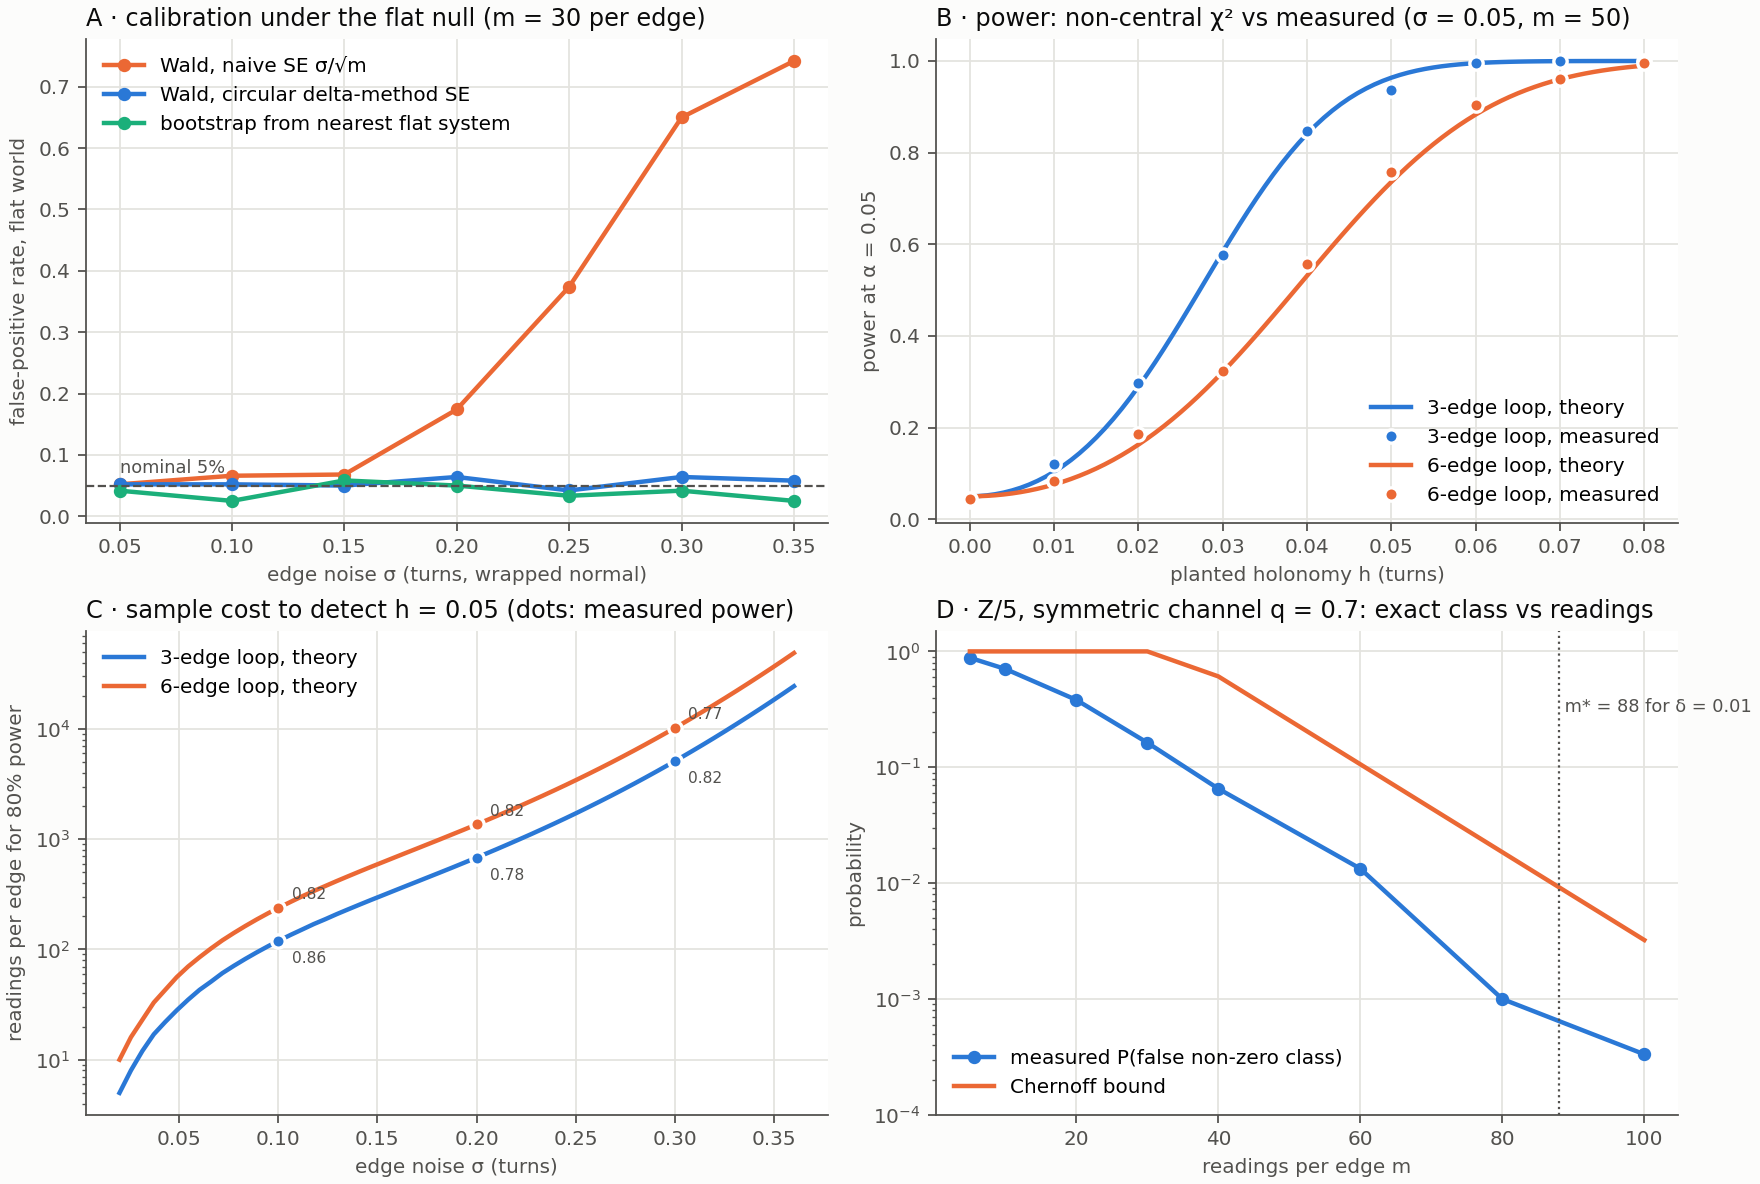
\includegraphics[width=\linewidth]{holonomy.png}
\caption{Problem 26 \src{S}. (A) calibration; (B) power against theory; (C) sample cost; (D) discrete class error against the Chernoff bound.}\end{figure}

%---------------------------------------------------------------------
\section{From operations to outcomes, around the probability layer}
\begin{theorem}[The operation-system model $e_g$]\label{thm:eg}\st{proved, computed}
For $(\Gamma,\Z/n,g)$, let the measurements be the vertex colours, the contexts the edges, and let $e_{ab}$ be uniform on $\{(x,x+g_{ab})\}$. Then:
\begin{enumerate}
  \item $e_g$ is strongly contextual iff $[g]\ne0$;
  \item for $[g]\ne0$, $\gamma(s)\ne0$ for every section over every nonzero coefficient ring;
  \item $e_g$ is an instance of an all-versus-nothing model over $\Z/n$ \cite{abklm15}.
\end{enumerate}
\end{theorem}
\begin{proof}
(1) A global section is exactly a global field.

(2) Take a compatible $R$-family with $r_{C_0}=s$. Its restrictions to vertices are functions $f_v:\Z/n\to R$. Each support is the graph of a bijection, so compatibility forces $f_b(y)=f_a(y-g_{ab})$. Propagating the delta function $f=\delta_{x_0}$ from $C_0$ around a loop with $h\ne0$ gives $\delta_{x_0}=\delta_{x_0+h}$, which is impossible when $R\ne0$.
\end{proof}
\begin{proposition}[Layer 2 is blind to {$[g]$}]\label{prop:blind-eg}\st{proved}
In $e_g$, every edge has $I(c_a;c_b)=\log n$ whatever $g$ is. More generally, any per-context functional invariant under relabelling outcomes (every Shannon or Tsallis functional) is unchanged by post-composing an edge with a permutation.
\end{proposition}
\noindent The ring-invariance in Theorem~\ref{thm:eg}(2) contrasts with the mod-3 grid, where $\gamma$ vanishes over $\Q$. Ring dependence of $\gamma$ is a property of the family, not of $\gamma$.

%---------------------------------------------------------------------
\section{Lossy operations}
Each edge carries a doubly stochastic channel $K$. Colours are uniform, so the Bayesian inverse is $K^\top$. The loop operator $M_L$ is the product around the loop, and the edge-context model $e_K$ has law $\tfrac1nK_{ab}$ on edge $(a,b)$.

\begin{proposition}[Character eigenvalues]\label{prop:eig}\st{proved}
For covariant channels $C_{\mu_e}S_{g_e}$ on a finite abelian $A$, every character $\chi$ is an eigenvector of $M_L$ with $\lambda_\chi=\big(\prod_e\hat\mu_e(\chi)\big)\chi(h)$. For the noisy shift $K=(1-\varepsilon)S_g+\varepsilon U$, $M_L=(1-\varepsilon)^{|L|}S_h+[1-(1-\varepsilon)^{|L|}]U$ and $\lambda_\chi=(1-\varepsilon)^{|L|}\chi(h)$.
\end{proposition}
\begin{corollary}\label{res:auto12}
The labelled eigenvalue is base-point free, and its phase is $\chi(h)$ when every $\hat\mu_e(\chi)$ is real and positive. The unlabelled multiset is base-point free for \emph{any} channels, since $AB$ and $BA$ share their nonzero spectrum, but on $\Z/p$ it sees only the order of $h$. Asymmetric noise adds its own phase: the readout is $2.285$ instead of $2$.
\end{corollary}
\begin{proposition}[Information closed forms]\label{res:auto13}\st{proved}
$I(c_a;c_b)=\log_2n+(1-\varepsilon+\tfrac\varepsilon n)\log_2(1-\varepsilon+\tfrac\varepsilon n)+(n-1)\tfrac\varepsilon n\log_2\tfrac\varepsilon n$. The loop-composite information is the same with $\varepsilon_L=1-(1-\varepsilon)^{|L|}$. Both are independent of $h$.
\end{proposition}

\begin{theorem}[Contextual fraction on a cycle]\label{thm:cfcycle}\st{proved}
On a cycle of length $L$ with noisy shifts and holonomy $h\ne0$ in a finite abelian $A$,
\[
\CF(e_K)=\max\!\Big(0,1-\frac{L\varepsilon}{2}\Big),
\]
independent of $|A|$ and of $h$.
\end{theorem}
\begin{proof}
\emph{Upper bound on NCF.} Weight each cell by its discrepancy $d=y-x-g$: $w(0)=0$, $w(-h)=1$, and $w=\tfrac12$ otherwise. Discrepancies sum to $-h\ne0$, so every colouring has weight at least 1. The dual value is $L\tfrac\varepsilon n(1+\tfrac{n-2}2)=\tfrac{L\varepsilon}2$.

\emph{Lower bound (packing).} Take colourings with one violation of discrepancy $-h$ (mass $\varepsilon/n$ per edge), and colourings with two violations $(a,-h-a)$ (mass $\varepsilon/(2n(L-1))$ per ordered edge pair), spread over translations. These fill every off-graph class exactly, and the on-graph load $\tfrac{L\varepsilon}2-\varepsilon(1-\tfrac1n)$ fits within the capacity $1-\varepsilon(1-\tfrac1n)$ iff $L\varepsilon\le2$.

\emph{Beyond the threshold.} The model is affine in $\varepsilon$ and non-contextual at $\varepsilon=2/L$ and at $\varepsilon=1$.
\end{proof}
\begin{theorem}[Any graph, lower bound]\label{thm:girth}\st{proved}
$\CF(e_K)\ge\max(0,1-\lmin\varepsilon/2)$, where $\lmin$ is the shortest simple cycle with nonzero holonomy.
\end{theorem}
\begin{observation}\label{res:auto14}\st{measured}
Equality holds in 44 configurations: $\theta$-graphs, $K_4$, shared edges, shared vertices, disjoint non-flat loops, and $\varepsilon\le0.8$. Only $\lmin$ matters, not the cycle basis. The general packing is \st{open}.
\end{observation}
\begin{counterexample}[What does not hold]\label{ce:info}\st{computed}
\begin{itemize}
  \item \emph{Information does not determine CF.} A 3-cycle and a 5-cycle over $\Z/3$ at $\varepsilon=0.2$ have the same per-edge information, but $\CF=0.70$ and $0.50$.
  \item \emph{Non-covariant noise is contextual on its own.} Flat systems reach $\CF$ up to $0.24$, and the phase readout of $h=2$ spreads over $[1.1,3.1]$.
  \item \emph{Entropy is not a function of Fourier moduli.} A homometric pair has identical $|\hat p|$ but $H=2.7714$ against $2.7689$ bits.
\end{itemize}
\end{counterexample}

\begin{table}[!htbp]\centering\small
\begin{tabular}{llll}
\toprule
layer & invariant & response to $\varepsilon$ & detects $h$ until\\
\midrule
1 & labelled eigenvalue of $M_L$ & modulus $(1-\varepsilon)^{|L|}$, phase fixed & $\varepsilon\to1$\\
2 & per-edge and loop $I$ & decreases, independent of $h$ & never\\
3 & $\CF$ & $1-\lmin\varepsilon/2$ & $\varepsilon=2/\lmin$\\
3 & $\gamma$ & support becomes full & $\varepsilon=0$ only\\
\bottomrule
\end{tabular}
\caption{The same noise acting on four invariants \src{S}.}
\end{table}

\begin{figure}[!htbp]\centering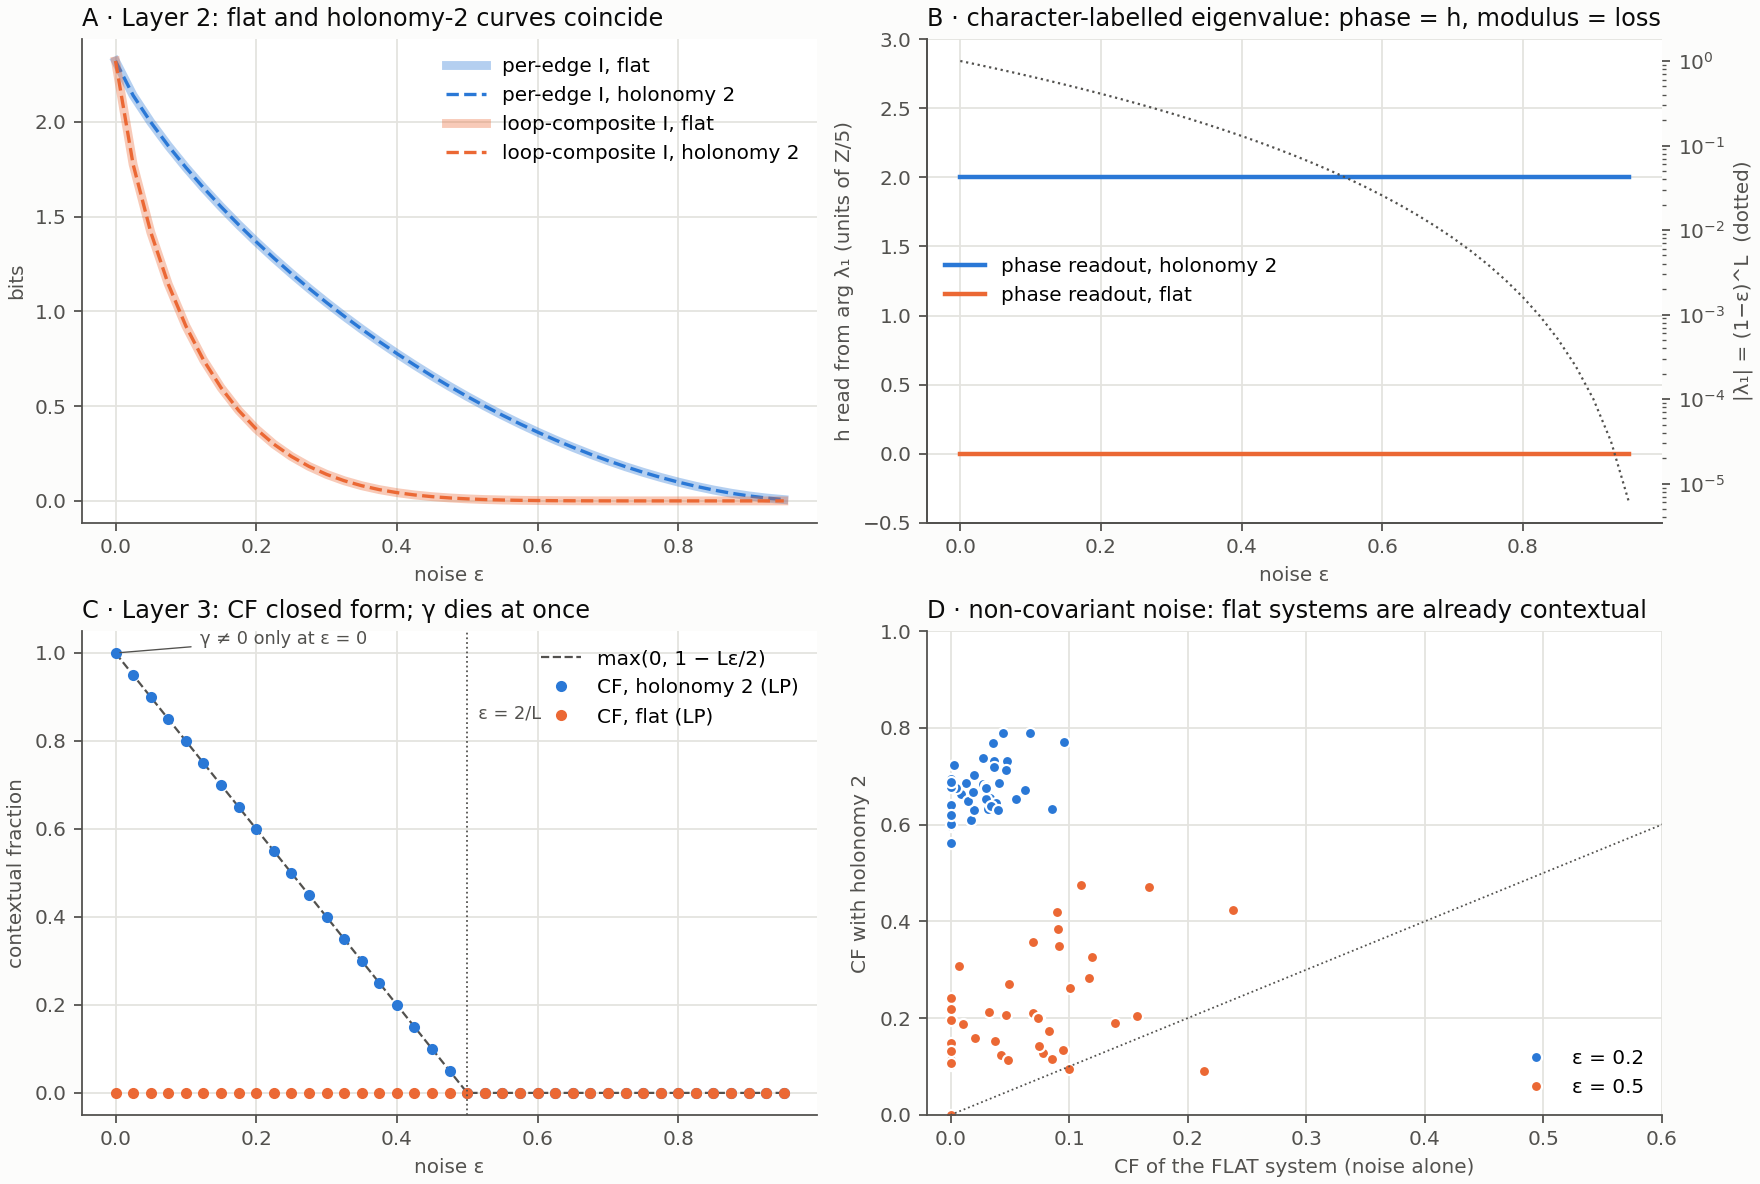
\includegraphics[width=\linewidth]{channels.png}
\caption{Noisy operations on a 4-cycle over $\Z/5$, with $h=2$ against a flat system \src{S}.}\end{figure}

\begin{proposition}[Orientation for $\Z/3$ and $\Z/5$]\label{res:auto15}\st{proved, computed}
For odd primes, $h\ne-h$ whenever $h\ne0$, so the labelled phase always detects orientation. Reversing the loop inverts the readout ($1\leftrightarrow4$ and $2\leftrightarrow3$ on $\Z/5$). The unlabelled multiset and $\CF$ do not detect orientation.
\begin{itemize}
  \item On $\Z/3$ a non-flat holonomy is exactly a chirality, read from the sign of $\operatorname{Im}\lambda_1$.
  \item On $\Z/5$ the phase splits into a magnitude class, $\operatorname{Re}\lambda_1/|\lambda_1|=0.309$ for $\pm1$ and $-0.809$ for $\pm2$, and an orientation.
  \item The magnitude class is meaningful only with fixed state labels, since $x\mapsto2x$ carries $h=1$ to $h=2$.
\end{itemize}
\end{proposition}

%---------------------------------------------------------------------
\section{The support dial: Tsallis entropies}\label{sec:tsallis}
\begin{proposition}\label{res:auto16}\st{computed; the cocycle property is Vigneaux's}
Let $S_\alpha=(1-\sum p^\alpha)/(\alpha-1)$ with the deformed action $(X\cdot_\alpha F)(P)=\sum_xP(X{=}x)^\alpha F(P\mid X{=}x)$.
\begin{itemize}
  \item $S_\alpha$ is a $\delta_\alpha$-cocycle (defect below $3\times10^{-15}$), but not a cocycle for Shannon's action (defect up to $1.8$).
  \item $S_0=|\mathrm{supp}|-1$, and $S_\alpha\to H$ as $\alpha\to1$.
  \item Mass $\epsilon$ added to an empty cell changes $S_0$ by 1, and $S_\alpha$ by $\sim\epsilon^\alpha$.
  \item $S(X)+S(Y)-S(XY)$ reaches $-1.71$ at $\alpha=0.5$.
\end{itemize}
$\alpha$ therefore interpolates between AMB's possibilistic lens ($\alpha=0$) and Shannon ($\alpha=1$). Every $S_\alpha$ is symmetric, so Proposition~\ref{prop:blind-eg} still holds.
\end{proposition}

%---------------------------------------------------------------------
\section{Support strata: where each lens can see anything}\label{sec:strata}
An empirical model $e=(e_C)_C$ lies in a product of simplices $\prod_C\Delta(O^C)$, intersected with the no-signalling polytope. Its \emph{support} is $\sigma(e)=(\operatorname{supp}e_C)_C$. The \emph{stratum} of $e$ is the set of models with the same support, that is, the relative interior of a face.
\begin{itemize}
  \item The \emph{interior} is full support in every context.
  \item The \emph{vertices} are one outcome per context.
\end{itemize}

\begin{proposition}[Support stratification]\label{prop:strata}\src{S}\st{proved}
\begin{enumerate}
  \item \emph{Face functions.} The support presheaf $\mathcal S_e$, its global sections, logical and strong contextuality, and $\gamma$ over every ring depend on $e$ only through $\sigma(e)$. Strong contextuality is inherited by smaller supports: if $\sigma(e)\subseteq\sigma(e')$ componentwise and $e'$ is strongly contextual, so is $e$.
  \item \emph{Interior.} With full support, every local section extends to a global section of $\mathcal S_e$. So $e$ is not logically contextual and $\gamma(s)=0$ for every $s$, over every ring. The contextual fraction can still be positive.
  \item \emph{Vertices.} If each $e_C=\delta_{s_C}$ and $e$ is no-signalling on a cover of the measurements, the $s_C$ glue to a global assignment $g$ with $e=\delta_g|_{\mathcal C}$. Then:
  \begin{itemize}
    \item $e$ is non-contextual, $\CF=0$ and $\gamma=0$;
    \item every Shannon and Tsallis functional of every context vanishes, together with every mutual and conditional information, since each is a combination of entropies of point masses.
  \end{itemize}
  \item \emph{The probability lens varies within strata.} $\CF$ is not a face function. It is convex (Abramsky--Barbosa--Mansfield), hence continuous on the relative interior of the model polytope. $S_\alpha$ for $\alpha>0$ and $H$ are continuous on closed simplices. $S_0=|\operatorname{supp}|-1$ is constant on strata and jumps exactly across them.
\end{enumerate}
\end{proposition}
\begin{proof}
\begin{enumerate}
  \item $\mathcal S_e(U)$ is the set of sections over $U$ whose restrictions to each context lie in $\operatorname{supp}e_C$. Every listed invariant is defined from $\mathcal S_e$. If $\sigma(e)\subseteq\sigma(e')$ then $\mathcal S_e\subseteq\mathcal S_{e'}$, so a global section of $\mathcal S_e$ is one of $\mathcal S_{e'}$.
  \item Extend $s\in O^C$ arbitrarily to $g\in O^X$. Every restriction of $g$ lies in a full support, so $g\in\mathcal S_e(X)$. A section that extends to a global section has trivial obstruction and is no logical witness.
  \item No-signalling gives $\delta_{s_C}|_{C\cap C'}=\delta_{s_{C'}}|_{C\cap C'}$, so $s_C|_{C\cap C'}=s_{C'}|_{C\cap C'}$. Because the contexts cover $X$, the $s_C$ glue to a unique $g$, and $\delta_g$ is a global law. $H(\delta)=S_\alpha(\delta)=0$ for all $\alpha$.
  \item The Tsirelson box and white noise lie in the same (interior) stratum, with $\CF=0.414$ and $0$. Continuity of $S_\alpha$ for $\alpha>0$ and the jump of $S_0$ are immediate from the formulas.
\end{enumerate}
\end{proof}

\begin{corollary}\label{res:auto17}\st{proved}
A nonzero $\gamma$ and logical contextuality occur only on \emph{intermediate} strata: neither full support nor single outcomes.
\begin{itemize}
  \item The PR box has no global section and 8 cohomological witnesses.
  \item The Hardy model has one logical witness, missed by $\gamma$ over $\Z$.
\end{itemize}
Contextuality in the interior is visible only to the probability lens ($\CF$); the possibilistic lens is blind to it. $S_0$ reads the stratum and $S_{\alpha>0}$ reads the position within it, which completes the support dial of Section~\ref{sec:tsallis}.
\end{corollary}

\begin{proposition}[Two-outcome supports are all-or-nothing]\label{prop:two}\src{S}\st{proved}
Consider a graph scenario with binary measurements and pairwise contexts. Let $e$ be no-signalling with $|\operatorname{supp}e_C|=2$ for every context.
\begin{enumerate}
  \item Every measurement is either \emph{pinned} (deterministic) or \emph{free} (both values occur). An edge between two free measurements has a bijection support $\{y=x+c_C\}$ with $c_C\in\Z/2$. An edge between a pinned and a free measurement has a product support. No edge joins two pinned measurements.
  \item $e$ is contextual if and only if the $\Z/2$ connection $c$ on the free subgraph has a non-flat cycle. It is then \emph{strongly} contextual, with $\CF=1$ and $\gamma\neq0$. Otherwise every local section extends and $\gamma=0$. Logical-but-not-strong contextuality, as in Hardy, needs a support of size at least 3.
  \item On a component with a non-flat cycle, no-signalling forces every free marginal to be $\tfrac12$, so the stratum is a single point there. On a flat component the stratum is a one-parameter family $q\in(0,1)$ with $\CF=0$.
  \item Per context, $H=I=h(q)$ and $S_0=1$. The non-flat point and the flat point $q=\tfrac12$ have identical per-context Shannon and Tsallis profiles, yet $\CF=1$ and $0$.
\end{enumerate}
\end{proposition}
\begin{proof}
\begin{enumerate}
  \item A size-2 subset of $\{0,1\}^2$ either fixes one coordinate or is the graph of a bijection. No-signalling makes pinned/free a property of the measurement.
  \item Global sections are the pinned values together with a flat section of the $\Z/2$ torsor on the free subgraph, which exists if and only if every cycle is flat. If no flat section exists, then $\mathcal S_e(X)=\emptyset$, and $\CF=1$ by Abramsky--Barbosa--Mansfield. If one exists, a torsor section is fixed by any one value on each component, so every local section extends.
  \item A bijection edge transports the marginal $p\mapsto p$ or $p\mapsto1-p$, and an odd cycle gives $p=1-p$.
  \item The joint on a bijection edge is determined by its marginal. Relabelling invariance gives the last claim, which is Proposition~\ref{prop:blind-eg} at $n=2$.
\end{enumerate}
\end{proof}
\noindent So at two outcomes, Layer~3 is exactly $\Z/2$ holonomy. The information lens sees only the free parameter $q$, and $q$ is pinned to $\tfrac12$ precisely when the holonomy is non-trivial.

\noindent\emph{Checked:} the CHSH parity family (\texttt{test\_two\_outcome\_supports\_all\_or\_nothing}):
\begin{itemize}
  \item flat models are non-contextual for $q=0.5,0.7,0.9$;
  \item the odd model at $q=0.9$ signals (defect $0.8$);
  \item at $q=\tfrac12$ the odd model is the PR box, with $\CF=1$ and a profile identical to the flat model's.
\end{itemize}

\begin{remark}[What this replaces]\st{withdrawn}
A proposed ``sheaf--geometric bridge'' identified $\gamma_{\mathrm{AMB}}$ with the boundary holonomy of a smooth circle bundle through a support-reduction functor $\chi$. It placed contextuality at single-outcome supports and tied it to the divergence of $\partial H/\partial p_i$ at $\partial\Delta$. It is rejected here, for four reasons:
\begin{itemize}
  \item Its central equation equates an integer class taken mod $\Z$, which is $0$, with a holonomy that is never defined.
  \item The AMB cover is a finite cover of a measurement set, not an open cover of a manifold, and $\chi$ is never constructed.
  \item Information cohomology uses measurable cochains and functional equations, so the divergence of a derivative cannot create a class. Its $H^{\ge2}$ is open, and ``$I=dH$'' conflates de Rham $d$ with $\delta$ and $\delta_t$ (we have $I=\delta_tH$).
  \item By Proposition~\ref{prop:strata}(3), single-outcome models are exactly where both lenses vanish.
\end{itemize}
The correct discrete statement relating holonomy and $\gamma$ is the connecting-class result for operation systems (Theorem~\ref{thm:eg}). The correct role of the simplex boundary is the stratification above.
\end{remark}
\noindent Checked in \texttt{tests/test\_strata.py}: interior (Tsirelson, noisy PR, noisy GHZ); vertices (random deterministic assignments on the CHSH, GHZ and $\Z/3$ grid scenarios); a CF-versus-face counterexample; and the intermediate faces.

%---------------------------------------------------------------------
\section{Magnitude and phase: what Layer 2 reads}\label{sec:magphase}
Proposition~\ref{prop:blind-eg} cannot be evaded by choosing a different symmetric functional. This section says what Layer~2 \emph{does} read, and how little must be added to recover $\CF$.

\begin{proposition}[Logical Bell bound]\label{prop:lbell}\src{S}\st{proved}
Let $\varphi_1,\dots,\varphi_n$ be formulas on contexts $C_1,\dots,C_n$ that are jointly unsatisfiable, as in Abramsky \cite{abramsky20}, and let $p_i=e_{C_i}(\varphi_i)$. Then $\CF(e)\ge\sum_ip_i-(n-1)$.
\end{proposition}
\begin{proof}
Write $e=(1-\lambda)e^{NC}+\lambda e'$ with $\lambda=\CF(e)$. A global assignment satisfies at most $n-1$ of the $\varphi_i$, so the non-contextual part contributes at most $n-1$ to $\sum_i p_i$, and the rest contributes at most $n$. Hence $\sum_ip_i\le(1-\lambda)(n-1)+\lambda n$.
\end{proof}
\noindent The bound costs linear time. A Liar cycle ($x_1=x_2,\dots,x_n=\neg x_1$) is the case of odd $\Z/2$ holonomy. For $n=4$ it is the PR box \cite{abramsky20}, which is Proposition~\ref{prop:two}.

\begin{proposition}[$\CF$ from moduli and one bit]\label{prop:modphase}\src{S}\st{lower bound proved; equality computed for $n=3,\dots,6$}
Take a binary $n$-cycle with uniform marginals and edge correlations $s_i=\mathbb E[(-1)^{a+b}]$.
\begin{enumerate}
  \item Layer~2 determines each modulus $|s_i|$ and nothing else about the $s_i$. The Shannon form is $I_i=\log2-h\bigl(\tfrac{1+|s_i|}2\bigr)$. The Tsallis-2 form, with Vigneaux's action, is $I_{2,i}=S_2(b)-a\cdot_2S_2(b)=(1+s_i^2)/4$. The signs are invisible by Proposition~\ref{prop:blind-eg}, and their product is the holonomy bit.
  \item The contextual fraction is
  \[
  \CF=\begin{cases}\max\bigl(0,\tfrac12(\sum_i|s_i|-(n-2))\bigr) & \text{odd holonomy,}\\[2pt]
  \max\bigl(0,\tfrac12(\sum_i|s_i|-2\min_i|s_i|-(n-2))\bigr) & \text{flat.}\end{cases}
  \]
  The right-hand side is a lower bound by Proposition~\ref{prop:lbell}, applied to the odd sign pattern that is best aligned with the $s_i$. Equality is computed for $n=4$: the LP agrees to $10^{-15}$ on 60 random models in \texttt{tests/test\_magnitude\_phase.py}, and on 300 in an exploratory run. For $n=3,4,5,6$ it agrees to $4\cdot10^{-16}$ on 160 random cycles (\texttt{tests/test\_weak\_edge.py}).
\end{enumerate}
\end{proposition}
\noindent\emph{Consequences.}
\begin{itemize}
  \item The holonomy bit moves $\CF$ by at most $\min_i|s_i|$. On 300 random CHSH models it moved $\CF$ by $0.078$ on average and by $0.82$ at most. With a noisy edge, Layer~2 alone nearly determines $\CF$.
  \item A flat cycle with one uniform edge ($|s_j|=0$) and the other edges perfect has $\CF=\tfrac12$.
  \item The Tsallis-2 form needs no inverse entropy: $|s_i|=\sqrt{4I_{2,i}-1}$. Independent bits give $I_2=\tfrac14$, not $0$, which is non-additivity. $S_2$ also has an exactly unbiased estimator, $\sum_xn_x(n_x-1)/N(N-1)$, so it avoids the Miller--Madow bias of plug-in Shannon estimates.
\end{itemize}

\begin{remark}[Grassmannian charts: magnitude is chart-invariant, phase is the chart coordinate]\label{rem:grass}\st{proved (identities); interpretation}
\begin{itemize}
  \item \emph{Exponential charts.} $\operatorname{Gr}(k,n)=GL_n/P$ has big cell $\exp(\mathfrak n^-)P$ with $\mathfrak n^-\cong\operatorname{Hom}(\F^k,\F^{n-k})$. For Grassmannians $\mathfrak n^-$ is abelian with $X^2=0$, so $\exp X=I+X$ and the chart $X\mapsto\operatorname{row}[I\mid X]$ is linear.
  \item \emph{Point counts.} Over $\F_q$, $|\operatorname{Gr}(k,n)|=\sum_\lambda q^{|\lambda|}=q^{k(n-k)}(1+O(q^{-1}))$.
  \item \emph{$S_2$ is a dimension.} For flags of type $k=(k_1,\dots,k_s)$,
  \[
  \dim\operatorname{Flag}(k)=\sum_{i<j}k_ik_j=\tfrac12\Bigl(n^2-\sum_ik_i^2\Bigr),\qquad\text{so}\qquad S_2(k/n)=\frac{2}{n^2}\dim\operatorname{Flag}(k)
  \]
  exactly. This underlies Vigneaux's limit $\tfrac{2}{n^2}\log_q\binom{n}{pn}_q\to S_2(p)$ \cite{vig}. Shannon entropy is the log of a set count, the multinomial, and $q\to1$ recovers it.
  \item \emph{Edges as chart points.} For the operation systems over $\F_p^k$, the support of edge $e$ is the graph of $G_e$, the point $\operatorname{row}[I\mid G_e]\in\operatorname{Gr}(k,2k)$. \emph{Its exponential coordinate is the operation $G_e$.} Affine maps are homogenised to $\F_p^{k+1}$.
  \item \emph{Two lenses.}
  \begin{itemize}
    \item Holonomy is the product of coordinates around a loop. The space of global sections has dimension reduced by $\operatorname{rank}(G_{\text{loop}}-I)$; for a translation by $h\neq0$ the loop matrix $\bigl(\begin{smallmatrix}1&h\\0&1\end{smallmatrix}\bigr)$ fixes 1 of 2 dimensions.
    \item Dimension, $S_2$ and entropy are $GL$-invariant, hence the same in every chart. That is Layer~2's blindness in geometric form.
    \item Chart invariants read magnitude (Layer 2). Coordinates composed around loops read phase (Layer 3).
  \end{itemize}
  \item \emph{Global structure.} No single chart covers $\operatorname{Gr}(k,n)$, and the transitions are non-linear (Pl\"ucker). The global invariants, Schubert classes and tautological Chern classes, live in the gluing, just as holonomy does.
\end{itemize}
\emph{Not claimed.} Vigneaux proves that differential entropy and dimension are the only degree-1 classes for Gaussian modules without coordinates. Whether dimension is a cocycle in a finite-field information structure built from our operation systems is settled in Proposition~\ref{prop:ffdim} below.
\end{remark}

\begin{proposition}[Dimension over $\F_p$]\label{prop:ffdim}\src{S}\st{proved; computed}
Laws on $\F_p^n$ whose support is an affine subspace form a sub-functor: it is closed under linear pushforward and under conditioning on a linear observable. On it, $D[X](P)=\log_p|\operatorname{supp}X_*P|$ is a 1-cocycle for the Shannon action,
\[
D[XY]=D[X]+\textstyle\sum_xP(x)\,D[Y](P\mid X=x).
\]
The reason is that every fibre $A\cap X^{-1}(x)$ is a coset of $A\cap\ker X$, so all fibres have the same dimension. On general laws the identity fails (defect up to $0.42$). The count $S_0=|\operatorname{supp}|-1$ is a cocycle for the $\alpha=0$ action on all laws.
\end{proposition}
\noindent\emph{Computed} (\texttt{magphase.py}, \texttt{tests/test\_magphase\_module.py}): 300 random affine-support laws on $\F_3^3$ with random linear observables give defect $\le7\times10^{-16}$; general laws give up to $0.42$.

\noindent\emph{Consequence.} Dimension is a Layer-2 cocycle in our finite-field setting, on affine supports. Its non-triviality would follow from the Baudot--Bennequin locality convention (local 0-cochains are constants), which we have not checked separately. Per edge it is constant, $D=1$ for every graph of a bijection of $\F_p$, so it is blind to holonomy, as Proposition~\ref{prop:blind-eg} requires. Holonomy appears only in the dimension of the \emph{glued} section space.

\paragraph{Dimension deficit from estimated supports.}\src{S}\st{measured}
Setup (\texttt{examples/dimension\_deficit.py}):
\begin{itemize}
  \item a 4-cycle over $\F_3$ and $\F_5$, with $N\in\{30,90,300\}$ samples per edge and symmetric noise $\varepsilon\in\{0.1,0.3\}$;
  \item edge supports thresholded at $\tau\in[0.2,0.6]$, and an edge accepted only if its support is the graph of an affine bijection;
  \item the loop map in homogeneous coordinates, and the statistic $\operatorname{rank}_{\F_p}(M_{\text{loop}}-I)$;
  \item a null band from a parametric bootstrap under the nearest flat system.
\end{itemize}
Three systems are planted:
\begin{itemize}
  \item \emph{flat}: deficit 0, $p$ global sections;
  \item \emph{translation holonomy}: deficit 1, 0 global sections, strongly contextual;
  \item \emph{multiplicative holonomy} ($a_{\text{loop}}=2$): deficit 1, exactly 1 global section (the fixed point), logically but not strongly contextual.
\end{itemize}
Findings:
\begin{itemize}
  \item Whenever all supports were recovered, the deficit was correct in every replicate. The null band was 0 at every $(\varepsilon,N,\tau)$.
  \item The statistic fails by \emph{abstaining}: at $\F_5$, $\varepsilon=0.3$, $N=30$, recovery is 2--9\%.
  \item $\gamma$ over $\Z$ and over $\Z/p$ agrees with the deficit in all six cases. The holonomy test covers only translations.
  \item The global-section count separates strong from logical contextuality, which the deficit alone does not.
\end{itemize}
\emph{Scope.} Under symmetric noise a failed recovery is a non-bijection, never a wrong bijection, so the null band is trivially 0. Non-covariant noise could produce wrong bijections and is untested.

\paragraph{Estimation: $S_2$ versus Shannon.}\src{S}\st{measured}
Moduli $|s_i|$ and $\CF$ of a binary 4-cycle were estimated from $N$ samples per edge, with 400 replicates for each of three configurations (\texttt{examples/s2\_vs\_shannon.py}). Four estimators were compared: unbiased $I_2$, Shannon plug-in, Miller--Madow, and the labelled sample correlation.
\begin{itemize}
  \item At $N\ge100$ all four agree to within $0.003$ in RMSE of $\CF$.
  \item At $N=30$ the $S_2$ route has the smallest bias in $s^2$ on weak edges ($0.017$ against $0.035$). It has the \emph{largest} $\CF$ RMSE on strong and near-threshold edges ($0.087$ against $0.067$, and $0.153$ against $0.125$), because $\CF$ needs $|s|=\sqrt{s^2}$ clipped to $[0,1]$.
  \item \emph{$S_2$ does not pay off here.} With uniform marginals, each $2\times2$ table has a one-dimensional sufficient statistic, the agreement count. Every lens is then a function of it, and unbiasedness of $s^2$ does not carry through the square root.
\end{itemize}

%---------------------------------------------------------------------
\section{A contradiction meter with provenance}\label{sec:meter}
\textbf{Input.} A claim $(u,i,j,r)$ means that provenance unit $u$ (a source, document or turn) asserts $x_i\oplus x_j=r$ about binary propositions. Claims may be single assertions (deterministic mode) or repeated samples.

\textbf{Three separate failures} \src{S}:
\begin{enumerate}
  \item \emph{Self-contradiction}: an odd cycle among one unit's own claims.
  \item \emph{Overlap disagreement} ($d^0\neq0$, the deficit): two units give the same edge different parities, significant at $z>3$ in sampled mode. It is recorded and the edge is \emph{not} glued.
  \item \emph{Contextuality across provenance} ($d^0=0$, $H^1\neq0$): the overlaps agree, but the glued graph has an odd cycle contained in no single unit. This is a Liar cycle (Proposition~\ref{prop:two}).
\end{enumerate}
Each cycle is reported with:
\begin{itemize}
  \item the logical-Bell lower bound on $\CF$ (Proposition~\ref{prop:lbell});
  \item a union-bound confidence that all of its parities are right;
  \item a blamed edge, only when every other edge comes from a declared trusted unit.
\end{itemize}
Coherent fabrications are invisible by construction.

\textbf{v1 changes} \src{S}:
\begin{enumerate}
  \item \emph{Pooled noise.} The flip rate $\hat\varepsilon$ is estimated by EM over all claims, with each edge's true parity latent. An edge's error probability is then the posterior $\lambda^{d}/(1+\lambda^{d})$, where $\lambda=\hat\varepsilon/(1-\hat\varepsilon)$ and $d$ is the majority margin. This replaces the worst-case binomial.
  \item \emph{Shortest odd cycles.} For every edge, the meter finds the shortest odd cycle through it by BFS in the parity double cover. It replaces fundamental cycles.
  \item \emph{Multiple testing.} Cycles are certified at level $\alpha/k$ over the $k$ candidates (Bonferroni).
\end{enumerate}

\textbf{Benchmark} \st{measured} (\texttt{examples/meter\_benchmark.py}).
\begin{itemize}
  \item \emph{Data}: 12 propositions and 4 honest units asserting 6 true parities each, with one added unit per scenario; 200 instances per cell. Results are in Table~\ref{tab:meter}.
  \item \emph{Pooling}: it fixes the $m=5$ row. At $\varepsilon=0.1$, self-contradictions go from $0.00$ to $0.78$ and cross-unit cycles from $0.33$ to $0.84$.
  \item \emph{Clean cases}: honest-only firing stays at or below $0.04$, and coherent fabrications are not flagged.
  \item \emph{Limits}: at $\varepsilon=0.2$ with $m\le5$, power is low.
  \item \emph{Validation}: \texttt{tests/test\_meter.py} checks the CF lower bound against the LP on 3- and 5-cycles.
\end{itemize}
\begin{table}[!htbp]\centering\small
\begin{tabular}{lccccc}
\toprule
$m$, $\varepsilon$, noise model & honest & self & overlap & cross (correct edge blamed) & fabrication\\
\midrule
1, 0 (deterministic) & 0.00 & 1.00 & 1.00 & 1.00 (1.00) & 0.00\\
5, 0.1, worst case & 0.00 & 0.00 & 0.74 & 0.33 (0.32) & 0.01\\
5, 0.1, pooled & 0.01 & 0.78 & 0.86 & 0.84 (0.84) & 0.01\\
3, 0.1, pooled & 0.04 & 0.37 & 0.61 & 0.55 (0.55) & 0.04\\
15, 0.2, pooled & 0.01 & 0.95 & 0.98 & 0.94 (0.94) & 0.00\\
5, 0.2, pooled & 0.04 & 0.21 & 0.56 & 0.19 (0.19) & 0.04\\
\bottomrule
\end{tabular}
\caption{Detection rates by planted scenario. The ``honest'' column is the false-positive rate of the full meter.}\label{tab:meter}
\end{table}

\paragraph{Relational claims: ``A said X'' and ``C caused D''.}\src{S}\st{measured} (\texttt{relclaims.py}, \texttt{examples/basil\_relational.py})
\textbf{Extraction.} Claims are extracted from spaCy dependency parses with transparent rules:
\begin{itemize}
  \item \emph{attribution}: a say-verb with a subject and a clausal complement, or ``according to''; deny, reject and dispute, or a negated verb, flip the polarity;
  \item \emph{causation}: cause, lead to, result in, trigger, spark, fuel, passive by-agents, and because of or due to; a negated verb flips the polarity.
\end{itemize}
\textbf{Stated axioms}:
\begin{itemize}
  \item A1: one statement has one speaker;
  \item A2: causation is not mutual;
  \item A3: there are no causal 3-cycles.
\end{itemize}
\textbf{Conflicts detected}:
\begin{itemize}
  \item \emph{polarity}: the same proposition asserted and denied;
  \item \emph{speaker}: A1 is violated;
  \item \emph{reversal}: A2 is violated;
  \item \emph{cycle}: A3 is violated by claims from two or more sources.
\end{itemize}
A speaker is used for A1 only when resolved. Role nouns, documents and channels (``the attorney'', ``the statement'', ``according to the Times'') are unresolved without coreference. Say-verbs nested in another say-verb's clause, and speakers inside quotations, belong to the outer speaker.

\textbf{Validation.} Ten planted mini-articles: one per conflict type, plus controls for a paraphrase, a causal chain, passive--active agreement, a role noun and a nested quote. All ten are classified correctly (\texttt{tests/test\_relclaims.py}).

\textbf{BASIL} (100 events, 3 outlets each).
\begin{itemize}
  \item \emph{Claims}: 1{,}667 attribution claims and 149 causal claims were extracted.
  \item \emph{Overlap}: only $43/1605$ attribution contents and $3/146$ causal pairs are made by two or more outlets in the same event. The opportunity to contradict is small, which is consistent with BASIL's finding that bias works through selection and framing.
  \item \emph{First pass}: 17 speaker flags, all reviewed by hand and none a contradiction. Thirteen were one person named two ways, two came from nested quotes, and two were different people saying similar lines.
  \item \emph{After resolution}: one flag, Lofgren against Pelosi on ``power grab''. These are two different quotes, and both can be true.
  \item \emph{Verdict}: no factual contradiction between outlets was found. The detector's value here is negative evidence, together with the overlap statistic. The rules are shallow, and recall on real text is unmeasured.
\end{itemize}

\paragraph{General binary claims.}\src{S}\st{proved (classification); computed}
Each unit's formulas define a local support $S_u\subseteq\{0,1\}^{C_u}$ (\texttt{meter\_general.py}; formula syntax: $\sim$, \&, $|$, $\hat{}$, $\to$, $\leftrightarrow$). A deletion-based minimal unsatisfiable set of units is classified as one of:
\begin{itemize}
  \item \emph{self}: $S_u=\emptyset$;
  \item \emph{overlap}: two units with disjoint projections onto their shared propositions;
  \item \emph{propagation}: arc consistency (semijoin reduction) empties a unit;
  \item \emph{cyclic}: arc consistency leaves every $S_u$ non-empty and consistent on overlaps ($d^0=0$), yet no global assignment exists.
\end{itemize}
By Beeri--Fagin--Maier--Yannakakis \cite{bfmy}, the cyclic type requires a cyclic hypergraph; this is the strongly contextual case. With assertion frequencies $p_u$, the core carries the logical-Bell bound $\CF\ge\sum p_u-(k-1)$.

\paragraph{Gaussian fast path over $\F_2$.}\src{S}\st{computed}
Weights of Gaussian type are closed under gluing, and gluing them is matrix algebra rather than a sum over assignments. The Grassmann--Gaussian weights of Korepanov and Sadykov \cite{korepanov}, whose 4-simplex weights are Grassmann--Gaussian exponents and whose Pachner-move relations are therefore algebraic identities between Gaussians, are an example of this principle; we use only this structural point, not their parameterisations. Over $\F_2$ the analogue is a unit whose support is an affine subspace, such as a parity, XOR or literal claim or a conjunction of these.
\begin{itemize}
  \item \emph{Method}: for such units, contradiction cores come from Gaussian elimination with row tracking. The combination $y$ with $yA=0$ and $yb=1$ is the certificate. A core is already minimal when $\operatorname{rank}=|\text{rows}|-1$ (a circuit); otherwise it is minimised by deletion.
  \item \emph{Timing}: brute force takes $0.35$\,s at 16 propositions and grows as $2^n$. The fast path handles a 5{,}000-claim Liar ring among 15{,}000 consistent distractor claims (20{,}000 propositions) in $0.66$\,s.
  \item \emph{Validation}: cores match brute force and are minimal on 40 random parity systems (\texttt{tests/test\_meter\_general.py}).
  \item \emph{Scope}: non-affine claims such as $A\to B$ keep the exact but exponential path. General satisfiability is NP-hard, and the $\CF$ LP is not reduced by this.
\end{itemize}

\paragraph{First real run: BASIL, overlap channel.}\src{S}\st{measured}
\textbf{Setup} (\texttt{examples/basil\_overlap.py}):
\begin{itemize}
  \item BASIL \cite{basil}: 97 events with all three outlets (Fox, NYT, HuffPost) annotated; gold annotations only.
  \item Sources are the outlets. A proposition is ``the article is negative toward target $T$ in event $t$''.
  \item Literals are encoded as parity edges to an anchor proposition, so cycles cannot arise and only the overlap channel is exercised.
  \item Null: outlet labels permuted within events, 1000 permutations.
\end{itemize}
\begin{table}[!htbp]\centering\small
\begin{tabular}{lcccc}
\toprule
reading & Fox--NYT & Fox--HPO & NYT--HPO & separation ($p$)\\
\midrule
A: article-level author feeling (deterministic) & 12/26 & 6/17 & 1/27 & $0.370$ ($0.002$)\\
B: phrase-level spans (sampled, $\hat\varepsilon=0.114$) & 11/112 & 9/115 & 7/113 & $0.026$ ($0.21$)\\
\bottomrule
\end{tabular}
\caption{Overlap disagreements over shared propositions. Separation is the mean Fox-versus-others rate minus the NYT--HPO rate.}
\end{table}
\begin{itemize}
  \item At the article level Fox separates from the other two ($p=0.002$). In span-level polarity it does not ($p=0.21$).
  \item Disagreeing article pairs have different annotated relative stance in 19/19 (A) and 26/27 (B) cases, against a base rate of $240/291$. The binomial tails are $0.026$ and $0.037$.
  \item \emph{Caveats.}
  \begin{itemize}
    \item Stance and feelings come from the same annotators, so the stance check is not independent.
    \item The counts are small: 17--27 shared propositions in reading A.
    \item These disagreements are differences in slant, recorded as overlap. They are neither factual contradictions nor hallucinations.
    \item Cycles need relational claims, which BASIL's annotations do not provide.
  \end{itemize}
\end{itemize}

One example in \texttt{tests/test\_meter\_general.py} matters for the attention proposals reviewed earlier: ``$A\to B$, $B\to C$, $C\to\neg A$'' is \emph{satisfiable} (take $A$ false), so it is not a contradiction. Adding the claim ``$A$'' produces a propagation-type core. The parity version, $A\leftrightarrow B$, $B\leftrightarrow C$, $C\leftrightarrow\neg A$, is cyclic.


%---------------------------------------------------------------------
\section{The decorated Bregman--\v{C}ech nerve}
Tokens are points $p_i\in\Delta(\text{states})$ with a time $\tau_i$. The radius of a simplex is $\min_c\max_i\KL(p_i\|c)$.

\begin{lemma}\label{res:auto18}\st{proved, computed}
The balls $\{p:\KL(p\|c)\le r\}$ are convex, since KL is convex in its first argument, so the nerve lemma applies. For a pair, the optimum lies on the segment between the two points; it is found by bisection and certified by the minimax dual $\max_\lambda[\lambda\KL(p\|m)+(1-\lambda)\KL(q\|m)]$ to $10^{-9}$.
\end{lemma}
\begin{construction}[Decoration]
\begin{itemize}
  \item Edges are oriented by time (``A before B'') and labelled by the best-aligning group element, with its margin over the runner-up.
  \item Triangles carry their boundary holonomy; a nonzero value is a non-flat event.
  \item Each $H_1$ bar is labelled by the holonomy of its birth cycle.
\end{itemize}
\end{construction}
\begin{proposition}[Invariants for $\Aff(\Z/p)$]\label{res:auto19}\st{proved}
Loop labels depend on the base point only by conjugation. The conjugacy classes are: the identity; all nontrivial translations, as one class; and one class per multiplier $u\ne1$. For odd $p$, $\Aff(\Z/p)^{ab}=(\Z/p)^\times$, so only $u$ is a function of the $H_1$ class. Relabelling tokens preserves the class and not the element (tested).
\end{proposition}
\begin{proposition}[Walls]\label{prop:walls}\st{proved; consequence measured}
A permutation $\sigma$ of $n$ states fixes a face of codimension $n-\#\text{cycles}(\sigma)$. In $\Aff(\Z/3)\cong S_3$ the reflections are transpositions, fixing codimension-1 walls. The quotient is a Coxeter chamber, and every planted holonomy is absorbed into a flat labelling (0/100 recovered). Every non-identity element of $\Aff(\Z/5)$ has codimension $\ge2$.
\end{proposition}
\begin{observation}\label{res:auto20}\st{measured}
On $\Aff(\Z/5)$, rings with every edge margin $\ge10^{-3}$ are recovered in 254/255 cases; rings with an ambiguous edge are wrong in 57/145. On $\Z/3$ translations, both orientations are recovered and reversing time inverts the label.
\end{observation}
\noindent\textbf{Limits} \st{measured}:
\begin{itemize}
  \item Dirichlet noise on tokens (concentration $2000\to200$) raises ring-label error from 15\% to 48--63\%.
  \item The $\Z/2$ barcode readout is confounded by shortcut loops of the quotient and by coefficients: 18/20 correct on $\Z/5$ translations and 8/12 on $\Z/3$.
  \item In the non-abelian case, bars with non-identity labels can die at flat triangles.
\end{itemize}
\noindent\textbf{Semantics adopted.} Negation is \emph{partial}: it is undefined on U and sends U to an explicit \emph{not-applicable} state. Operations therefore form an inverse monoid, not a group, and are lossy.

%---------------------------------------------------------------------
\section{Two facets: restriction and extension}\label{sec:functors}
Let $i:\Sigma\to\mathcal S$ include the cover into the information site.
\begin{proposition}\label{res:auto21}\st{proved, computed}
\begin{enumerate}
  \item \emph{Restriction} $R$: $P\mapsto(\pi_C P)_C$ has image exactly the non-contextual models.
  \item \emph{Extension} $E$: $e\mapsto\mathrm{Ext}(e)=\{P:R(P)=e\}$ is a convex polytope, nonempty iff $\CF(e)=0$. If $\CF=0$, there is $b\ge0$ with $\sum b=1$ and $R(b)\le e$, and equal context totals force $R(b)=e$.
  \item $P\in E(R(P))$, and $R(E(e))=\{e\}$ whenever $E(e)\ne\emptyset$.
  \item The canonical member of $E(e)$ is the maximum-entropy extension, found by iterative proportional fitting (Csisz\'ar). IPF fails to converge on contextual models.
\end{enumerate}
\end{proposition}
\begin{observation}[Graded extension]\label{res:auto22}\st{measured}
The optimal non-contextual parts, of mass $1-\CF$, form a face. In CHSH it is a single point for every contextual model tested (39/39); in the three-party GHZ scenario it never is (0/10). The maximum-entropy point of the face gives a unique representative.
\end{observation}
\noindent These maps act on models, not on cohomology, so they are consistent with Theorem~\ref{thm:nonunif}. The attached drafts' forward map, which sent $\gamma/\CF$ to the spectral modulus, is not a functor.

%---------------------------------------------------------------------
\section{Not-applicable entries: the gated test}\label{sec:na}
Records are windows of labels (T, F, could-T, could-F, U, n/a), with a \emph{mask} marking variables that are not in the context. The mask is distinct from the \emph{n/a value}.

\begin{construction}[Pipeline]
\begin{enumerate}
  \item GYO reduction of the maximal observed contexts. If the cover is acyclic, the pipeline stops (Theorem~\ref{thm:vorobev}); any $\CF>0$ is then inconsistency, not contextuality.
  \item Possibilistic test across support thresholds, with its null band.
  \item $\CF$ by LP, with the signalling defect reported beside it.
  \item Null: each record keeps its mask, and its values are redrawn from the maximum-likelihood consistent law. That law is found by missing-data EM (Theorem~\ref{thm:em}) and pinned to maximum entropy.
\end{enumerate}
\end{construction}
\begin{table}[!htbp]\centering\small
\begin{tabular}{llll}
\toprule
stream & gate & $\CF$ & verdict\\
\midrule
random N/A, complete records present & acyclic & --- & stop: the AMB half is empty\\
honest, one N/A per record & cyclic & 0.029 & null mean 0.027, $p=0.39$: stop\\
structured, shift twist & cyclic & 0.858 & above all 30 null replicates (max 0.044)\\
structured, negation with U$\to$n/a & cyclic & 0.859 & above the null, but signalling 0.18\\
\bottomrule
\end{tabular}
\caption{The gated test on 9{,}000-record streams \src{S}.}
\end{table}
\begin{proposition}[The deficit]\label{res:auto23}\st{proved (zero set); measured (the rest)}
The \emph{deficit} is the per-record log-likelihood lost by the best consistent law, $\min_P\sum_C w_C\KL(e_C\|P_C)$.
\begin{itemize}
  \item \emph{Zero set.} For no-signalling tables it vanishes iff $\CF=0$: the minimum is attained, and KL is zero iff the tables coincide.
  \item \emph{Not a function of CF.} At $\CF=0.5$ on noisy-shift cycles it is $0.101,0.068,0.051$ for $L=3,4,5$.
  \item \emph{Closed form at $\varepsilon=0$:} it equals $\log(L/(L-1))$ (measured to $10^{-4}$).
  \item \emph{Sampling floor.} On honest data it falls as about $1/N$ ($0.0079$, $0.0010$, $0.00015$ for $N=10^3,9\cdot10^3,8.1\cdot10^4$); on contextual data it stays flat at about $0.282$.
  \item \emph{Bootstrap intervals:} $[0.270,0.287]$ for the shift twist and $[0.291,0.309]$ for the negation twist.
\end{itemize}
\end{proposition}
\begin{observation}[The ridge]\label{res:auto24}\st{measured}
When contexts are pairs, the three-way interaction is unidentified. EM from different starts reaches the same likelihood with laws $0.005$--$0.023$ apart in $L_1$. This is the upper-level identifiability failure of Part~I in three variables. The maximum-entropy pin removes the start dependence (tested); without it, a null on larger contexts would measure ridge drift.
\end{observation}
\begin{observation}[Thresholded $\gamma$]\label{res:auto25}\st{measured}
Near a cell's expected mass, sampling flips cells in and out of the support and manufactures logical witnesses. The null fires in 20/20 replicates at threshold $0.005$ on honest data, and at $0.1$ on the contextual streams' null. $\gamma$ is admissible only where the null band is near zero: at $0.02$ and $0.15$, both structured streams give $\gamma\ne0$ at $5/5$ against a null of $0/20$. Report the full sweep.
\end{observation}

\section{O2: when is a merged model minimal sufficient?}\label{sec:o2}
Fix a level $l$ of a binary tree grammar and one node $n$ at that level. Write $B\in[V]$ for its symbol, $X$ for the leaves of its subtree and $O$ for all other leaves. The grammar gives $X\perp O\mid B$, so
\[
P(x,o)=\sum_b P(b)\,D[b,x]\,U[b,o],\qquad D[b,x]=P(x\mid b),\quad U[b,o]=P(o\mid b).
\]
A \emph{partition merge} $f:[V]\to[V']$ replaces $B$ by $f(B)$ and pools rows with weights $P(b\mid f(B))$. It is \emph{exact} if $X\perp O\mid f(B)$, so the merged model reproduces the law of $(X,O)$.

\begin{proposition}[Lossless merges]\label{prop:o2a}\src{S}\st{proved}
A block $S$ of $f$ is exact if either
\begin{enumerate}
  \item[(i)] the downward rows $D[b]$, $b\in S$, are equal (in particular, if the child rows $R_l[b]$ are equal), or
  \item[(ii)] the upward rows $U[b]$, $b\in S$, are equal.
\end{enumerate}
\end{proposition}
\begin{proof}
The block contributes $M_S=\sum_{b\in S}P(b)D[b]U[b]^{\top}$ to $P(X,O)$. Under (i), $M_S=d_S\,(\sum_{b\in S} P(b)U[b])^{\top}$. Under (ii), $M_S=(\sum_{b\in S}P(b)D[b])\,u_S^{\top}$. Either way $M_S=P(S)\,P(X\mid S)\,P(O\mid S)^{\top}$.
\end{proof}

\noindent Case (ii) is exact at a position. In a grammar with one table per level it needs $P(b\mid f(B))$ to be the same at every node of the level. This holds automatically at the root, which is a single node.

\begin{proposition}[The minimal sufficient statistic is a rank object]\label{prop:o2b}\src{S}\st{proved}
\begin{enumerate}
  \item The minimal sufficient statistic of $X$ for $O$ is $x\mapsto P(O\mid x)=q(x)^{\top}U$, where $q(x)=P(B\mid x)$. Equivalently it is $q(x)$ modulo $\ker U^{\top}$.
  \item Its values span a space of dimension $r^*=\operatorname{rank}P(X,O)=\operatorname{rank}(G^{1/2}K^{1/2})$, where $G=DD^{\top}$ is computed by the recursion $G_l=R_l(G_{l-1}\otimes G_{l-1})R_l^{\top}$ and $K$ is the outside Gram.
  \item Any exact merge has $V'\ge r^*$.
\end{enumerate}
\end{proposition}
\begin{proof}
\begin{enumerate}
  \item $P(o\mid x)=\sum_b P(b\mid x)U[b,o]$ by the Markov property. Minimality is the standard likelihood-ratio characterisation.
  \item $P(X,O)=\operatorname{diag}(p_X)\,[P(O\mid x)]_x$, so the span of the $P(O\mid x)$ has dimension $\operatorname{rank}P(X,O)$. Write $D=G^{1/2}W$ and $U'=K^{1/2}W'$ with $W,W'$ row-orthonormal on the relevant ranges. Then $P(X,O)=W^{\top}G^{1/2}K^{1/2}W'$.
  \item An exact merge factors $P(X,O)$ through $V'$ states.
\end{enumerate}
\end{proof}

\begin{theorem}[When a partition reaches the minimum]\label{thm:o2c}\src{S}\st{proved}
Suppose the rows $D[b]$ are linearly independent.
\begin{enumerate}
  \item A block $S$ is exact if and only if $U[b]$ is constant on $S$.
  \item A partition merge attains $V'=r^*$ if and only if the number of distinct upward rows equals $\operatorname{rank}U$. That is, the whole rank deficiency of $U$ must come from equal rows.
\end{enumerate}
\end{theorem}
\begin{proof}
With $D_S$ the matrix of rows $D[b]$, $b\in S$, we have $M_S=D_S^{\top}W_S$ with $W_S$ having rows $P(b)U[b]$. Since $D_S$ has independent rows, $\operatorname{rank}M_S=\operatorname{rank}W_S$. This is 1 if and only if the $P(b)U[b]$ are proportional, that is, the probability vectors $U[b]$ are equal. The coarsest exact partition is therefore ``equal upward rows''. Its size is the number of distinct rows, while $r^*=\operatorname{rank}D^{\top}\operatorname{diag}(P(b))U=\operatorname{rank}U$.
\end{proof}

\begin{counterexample}\label{ce:o2}\st{computed}
Take $V=3$ with independent $D$, and $U[c]=\tfrac12(U[a]+U[b])$ with $U[a]\neq U[b]$. Then $r^*=2$, but none of the three 2-block partitions is exact. The minimal sufficient statistic $q_a+\tfrac12 q_c$ mixes symbols fractionally, so no merge can produce it. This is checked in \texttt{tests/test\_o2.py}.
\end{counterexample}

\begin{proposition}[Bregman cost is a complete-data quantity]\label{prop:o2d}\src{S}\st{proved}
The split--merge cost of merging a block $S$ is $\sum_{b\in S}n_b\,\mathrm{KL}(R_l[b]\,\|\,\bar R_S)=n_S\,I(B;\text{children}\mid B\in S)$. It vanishes if and only if case (i) holds. It is blind to case (ii): an upward-exact merge has zero observed-data loss but positive cost whenever the child rows in $S$ differ.
\end{proposition}
\begin{proof}
The identity is the Bregman-information form of the mutual information, as in Banerjee et al.\ \cite{banerjee}. Zero-loss under (ii) is Proposition~\ref{prop:o2a}.
\end{proof}

\begin{corollary}[The root collapses]\label{res:auto26}\st{proved}
The root has an empty outside, so $U$ has rank 1 and every root partition is exact. The root can always be replaced by one symbol with coupling $\mu(u,v)=\sum_b\pi_bR_L[b,u,v]$, since $P(x)=\sum_{u,v}\mu(u,v)\beta_u\beta_v$. The complete-data cost of this collapse is $I(B_{\mathrm{root}};\text{children})>0$.
\end{corollary}

\paragraph{Corpus B, true grammar.}\st{computed}\ Corpus B was regenerated with the builder's flags. The rules are identical, because they are drawn before sampling.
\begin{table}[!htbp]\centering\small
\begin{tabular}{lccccc}
\toprule
level & reachable $V$ & distinct child rows & $\operatorname{rank}D$ & distinct upward rows & $r^*$\\
\midrule
1 (left, right) & 7 & 7 & 7 & 7 & 7\\
2 (left, right) & 8 & 8 & 8 & 8 & 8\\
3 (left, right) & 8 & 8 & 8 & 8 & 8\\
4 (root) & 8 & 8 & 8 & 1 & 1\\
\bottomrule
\end{tabular}
\caption{O2 ranks on the true grammar of Corpus B (\texttt{examples/o2\_ranks.py}).}
\end{table}

\noindent Level-1 symbol 2 is never produced by a level-2 rule. A first pass that kept it showed $r^*=7<8$ with 8 distinct rows. That is unreachability, not a non-partition deficiency.

By Theorem~\ref{thm:o2c}:
\begin{itemize}
  \item At levels 1--3 no nontrivial exact merge exists, and the reachable true grammar is already minimal sufficient.
  \item At the root the minimum is 1.
\end{itemize}

\noindent On the regenerated validation split (2000 sequences):
\begin{itemize}
  \item the 8-symbol root and the single $\mu$-root give identical held-out $\log p$ per sequence, $-15.282238$ (difference $0$ to machine precision);
  \item the complete-data cost of the collapse is $1.799$ nats per root node;
  \item across all 127 two-block root partitions the cost ranges over $[1.106,1.563]$ nats, while the observed loss is exactly $0$ for every one.
\end{itemize}

\noindent This explains the level-4 anomaly in \src{H}: merging $8\to2$ at the root cost $0.72$ nats/node yet improved held-out likelihood. Proposition~\ref{prop:o2d} predicts exactly this, and it is why split--merge must accept merges on held-out likelihood rather than on cost.

\paragraph{Status of O2.}
\begin{itemize}
  \item Settled for the true grammar: the characterisation (Theorem~\ref{thm:o2c}), the bound $V'\ge r^*$, and the Corpus B verdict.
  \item Open: the same test on fitted tables, where exact equalities become statistical ones. A test for equal upward rows needs an outside-Gram estimator and a null, in the same pattern as V6.
  \item Open: whether real corpora exhibit Counterexample~\ref{ce:o2}. That would require a soft, non-partition compression.
\end{itemize}

\section{Experiment: grammar-guided transformers on Corpus B}\label{sec:exp1}
\textbf{Question.} Does the split--merge grammar help a transformer beyond what the transformer learns alone?

\textbf{Setup} \src{S} \st{measured}.
\begin{itemize}
  \item Corpus B: 19{,}000 training sequences, 1{,}000 for early stopping, and the 2{,}000-sequence validation split.
  \item The grammar is fitted by split--merge (3 rounds) and scores $-15.421$ against the truth's $-15.282$.
  \item The model is a causal transformer with $d=64$ and 4 heads, trained for 4{,}000 AdamW steps at batch size 256.
  \item The guidance is the fitted grammar's prefix posteriors $P(B_\ell(t)\mid x_{<t})$ of the four ancestors of the next leaf, computed by inside--outside with unobserved leaves set to 1.
  \item Variants:
  \begin{itemize}
    \item \emph{base}: no guidance;
    \item \emph{aux}: auxiliary heads distil the posteriors, and nothing is used at test time;
    \item \emph{feed}: the log-posteriors are added to the input embedding, so the grammar is used at test time.
  \end{itemize}
  \item \emph{Oracle} rows use posteriors from the true grammar.
  \item The metric is held-out excess NLL over the true grammar, in nats per sequence. It is split by the level of the lowest common ancestor of leaves $t-1$ and $t$.
\end{itemize}
\begin{table}[!htbp]\centering\small
\begin{tabular}{lcccccc}
\toprule
model & total excess & lvl 1 & lvl 2 & lvl 3 & lvl 4\\
\midrule
fitted grammar alone & 0.139 & 0.028 & 0.096 & 0.011 & 0.004\\
base, 2 layers (seeds 0, 1; 8k steps) & 0.454, 0.490; 0.464 & 0.14--0.17 & 0.18--0.19 & 0.12 & 0.01--0.02\\
base, 4 layers & 0.369 & 0.129 & 0.125 & 0.090 & 0.023\\
aux, 2 layers (seeds 0, 1) & 0.267, 0.299 & 0.07--0.08 & 0.11--0.13 & 0.06--0.08 & 0.01--0.02\\
aux, 4 layers & 0.274 & 0.084 & 0.113 & 0.057 & 0.014\\
feed, 2 layers (seeds 0, 1) & 0.145, 0.093 & 0.02--0.04 & 0.03--0.06 & 0.03 & 0.01--0.02\\
feed, 4 layers & 0.099 & 0.024 & 0.034 & 0.031 & 0.008\\
oracle aux / oracle feed, 2 layers & 0.269 / 0.132 & --- & --- & --- & ---\\
\bottomrule
\end{tabular}
\caption{Excess NLL over the true grammar on 2{,}000 validation sequences. The standard error of a total is about $0.01$--$0.02$.}
\end{table}

\noindent\textbf{Findings.}
\begin{itemize}
  \item \emph{The baseline is data-limited, not undertrained.} Doubling the steps changes nothing ($0.454\to0.464$). Its largest deficits are at the level-2 and level-3 boundaries, where the fitted grammar's level-3 excess is 11 times smaller.
  \item \emph{Distillation helps without using the grammar at test time.} The paired difference is $-0.187\pm0.021$ at 2 layers and $-0.096\pm0.021$ at 4 layers, and the level-3 deficit falls by about 40\%. Oracle targets give the same result ($0.269$). So the gain is not limited by the quality of the fit.
  \item \emph{Feeding the posteriors reaches the grammar, not beyond.} Against the grammar alone the paired differences are $-0.046\pm0.013$, $+0.006\pm0.014$ and $-0.040\pm0.013$. Even oracle posteriors leave $0.13$ nats, which is the cost of the transformer's read-out.
  \item The transformer improves on the grammar's level-2 error and loses at levels 3--4.
\end{itemize}

\noindent\textbf{Scope.}
\begin{itemize}
  \item One corpus in the identifiable regime (781 observations per parameter at level 3).
  \item One fit; two seeds at 2 layers and one at 4.
  \item Corpus A is untested. There the fit itself fails at level 3, and guidance cannot supply what the fit lacks.
  \item Not tested: the specific proposal of Bregman-merge E-steps on hidden states with a multiplicative attention mask. Section~\ref{sec:o2} argues against its merge criterion.
\end{itemize}

\section{Experiment: recursive training (model collapse) on Corpus B}\label{sec:collapse}
\textbf{Question.} Can the support dial serve as a label-free collapse metric? Does the small-$\alpha$ lens see collapse before Shannon entropy or likelihood?

\textbf{Setup} \src{S} \st{measured}.
\begin{itemize}
  \item Generation 0 is the split--merge fit on real data.
  \item Each generation samples $N$ sequences from the current model and refits by EM (30 sweeps, warm-started).
  \item Three arms:
  \begin{itemize}
    \item \emph{replace}: train on the newest synthetic sample only;
    \item \emph{accumulate}: train on real data plus all synthetic samples so far;
    \item \emph{fresh}: each generation trains on fresh real data. This is the null, and it has the same retraining noise with no feedback loop.
  \end{itemize}
  \item Metrics, computed on 20{,}000 model samples of 8-leaf blocks:
  \begin{itemize}
    \item $S_\alpha$ for $\alpha\in\{0,0.5,1,2\}$;
    \item recall of the true block support and of its rarest half, the tail;
    \item held-out log-likelihood of \emph{real} data.
  \end{itemize}
\end{itemize}
\begin{table}[!htbp]\centering\small
\begin{tabular}{lcccc}
\toprule
$N=1000$, generation 20 & $\log p$ (real) & $S_0$ of 8-blocks & Shannon $H$ & tail recall\\
\midrule
generation 0 & $-15.421$ & 4206 & 8.072 & 0.977\\
replace & $-17.266$ & 3716 ($-11.7\%$) & 7.801 ($-3.4\%$) & 0.842\\
accumulate & $-15.453$ & 4141 & 8.041 & 0.970\\
fresh (null, generation 19) & $-15.451$ & 4185 & 8.058 & 0.974\\
\bottomrule
\end{tabular}
\caption{Collapse under replacement, with none under accumulation or fresh data. At $N=4000$ replacement collapses more slowly: $\log p$ goes from $-15.421$ to $-15.629$ and tail recall from $0.977$ to $0.972$ after 20 generations, while accumulation stays at $-15.434$. At $N=20{,}000$, six generations move $\log p$ by only $0.011$.}
\end{table}

\textbf{Which lens first?} A generation is flagged when its change from generation 0 falls below $-3$ times the RMS drift of the fresh arm (\texttt{collapse\_analysis2.py}).
\begin{itemize}
  \item Under replacement, $S_0$, $S_{0.5}$, $H$, $S_2$ and $\log p$ on real data are \emph{all} flagged at generation 3. The accumulate arm is flagged 0 of 20 times by every metric.
  \item At generation 20 the $z$ values are: $S_0$ $-15.0$, $S_{0.5}$ $-14.6$, $H$ $-15.0$, $S_2$ $-18.6$, $\log p$ $-48.5$, tail recall $-18.5$.
  \item The largest \emph{relative} change is in $S_0$ ($-11.7\%$, the fraction of distinct block types lost). This matches the tail-recall loss ($-13.8\%$) and the likelihood loss.
  \item \emph{The hypothesis that the support lens detects collapse earlier is not supported.} Every order of $\alpha$ detects at the same generation. $S_0$ is the most interpretable reading and $S_2$ the most precise.
  \item A naive null that uses sampling noise alone, with no refitting, makes $H$ and $S_2$ flag the harmless drift of the accumulate arm. The retraining null is necessary.
\end{itemize}
\emph{Scope.}
\begin{itemize}
  \item One synthetic grammar and one generation-0 fit. The generation-0 model carries spurious mass (precision $0.963$), and early generations shed some of it.
  \item This is a corpus-level signal, not per-document detection of machine text.
\end{itemize}

\section{Experiment: unknown branching (Corpus V)}\label{sec:vbranch}
\textbf{Grammar} \src{S}. Every production is $b\to c_0\,c_1\cdots c_k$: one left child, and $k\in\{0,\dots,5\}$ right children. The depth is fixed ($L=3$), with $V=8$ symbols, $A=12$ leaves and $m=3$ productions per symbol. Each production draws its own $k$, so sentence length varies (mean $77$, range $3$--$149$) and the tree is hidden.

\textbf{Exact inference.} Store each symbol as a span matrix, $B[i,j]=P(\text{symbol yields }x_{i:j})$.
\begin{itemize}
  \item Concatenating children is a matrix product: $B_l[b]=\sum_rp_r\,B_{l-1}[c_0]\cdots B_{l-1}[c_k]$.
  \item A sparse chart version gives exact inside--outside in $1.7$\,ms per sentence.
  \item It agrees with brute-force enumeration to $10^{-16}$, and expected counts agree with finite differences.
  \item Every validation sentence has exactly one derivation under the true grammar. The true log-likelihood is $-30.87$ nats per sentence ($0.40$ per token).
\end{itemize}

\textbf{Learners} (head plus right children; banded span tables; EM with autodiff expected counts; checked against brute force):
\begin{itemize}
  \item \emph{Markov}: $k\sim K[b]$, $c_0\sim H[b]$, $c_t\sim R[b,c_{t-1}]$.
  \item \emph{Positional}: $k\sim K[b]$, $c_0\sim H[b,k]$, $c_t\sim R[b,k,t]$. It contains the true grammar except where a symbol has two productions with the same $k$; there are 13 such collisions over the three levels.
\end{itemize}
\begin{table}[!htbp]\centering\small
\begin{tabular}{lc}
\toprule
model (1000 training sentences) & held-out $\log p$ / sentence\\
\midrule
true grammar & $-30.87$\\
positional, from gold trees (an EM fixed point) & $-42.71$\\
Markov, from gold trees (3 EM sweeps: $-82.19$) & $-82.56$\\
positional, EM from random, 20 sweeps (seeds 0, 1) & $-82.80$, $-90.43$\\
bigram / unigram & $-151.9$ / $-189.2$\\
\bottomrule
\end{tabular}
\caption{Corpus V \st{measured}.}
\end{table}

\noindent\textbf{Chunks and split--merge} \st{measured} (\texttt{vchunks.py}, \texttt{vsplitmerge.py}).
\begin{itemize}
  \item \emph{Chunk induction}, level by level:
  \begin{enumerate}
    \item candidate substrings of length at most 6;
    \item EM for a unigram chunk model over segmentations;
    \item pruning of chunk types that are concatenations of other types, which counters the bias toward under-segmentation;
    \item spectral clustering by neighbouring chunks.
  \end{enumerate}
  \item \emph{Level 1}: all 24 true productions are recovered, with token precision 1 and cluster purity 1. \emph{Level 2}: all 24 productions are recovered with precision 1, but one true symbol is split across two clusters and two true symbols share a cluster.
  \item \emph{The grammar}: productions are read off the chunks, and the root is collapsed to one symbol, which is lossless by the root corollary of Section~\ref{sec:o2}. It scores $-31.77$, parses every held-out sentence, and EM leaves it unchanged.
  \item \emph{Split--merge}: splits and merges of symbol assignments, accepted only when exact held-out likelihood improves. Three moves bring it to $-30.91$, against the truth's $-30.87$.
  \item \emph{Residual error}: every final cluster is pure, but one true symbol stays split in two. At 500 held-out sentences, likelihood does not separate this nearly lossless split, as Section~\ref{sec:o2} would predict. A parsimony tie-break would settle it.
\end{itemize}
\begin{table}[!htbp]\centering\small
\begin{tabular}{lc}
\toprule
learner (1000 training sentences) & held-out $\log p$ / sentence\\
\midrule
true grammar & $-30.87$\\
\textbf{chunks + split--merge} & $\mathbf{-30.91}$\\
chunks only & $-31.77$\\
positional, from gold trees & $-42.71$\\
positional, EM from random & $-82.80$\\
\bottomrule
\end{tabular}
\caption{Corpus V: bottom-up chunk induction removes the basin problem.}
\end{table}

\noindent\textbf{Findings.}
\begin{itemize}
  \item \emph{Model class.} A production's children form a fixed tuple, so a first-order chain loses $51.7$ nats per sentence even with gold trees. Conditioning on arity and position loses $11.8$, which comes from the arity collisions.
  \item \emph{Search.} EM from random starts climbs well past the bigram, but after 20 sweeps it sits about 40 nats below the best model in its own class. That is the basin-selection problem of Corpus B again, and it motivates split--merge or chunk-based initialisation.
\end{itemize}

\section{Monodromy: representations of $\pi_1$ and twisted cohomology}\label{sec:mono}
\textbf{Construction} \src{S} (\texttt{monodromy.py}). Transport along an edge $a\to b$ is the conditional expectation $T_{ab}[x,y]=P(b=y\mid a=x)$. Composing around the fundamental cycles gives
\[
\rho:\pi_1(\Gamma)=F_{\beta_1}\to\mathrm{End}(\mathbb C^n).
\]
It is unitary exactly when every edge is a bijection; lossy edges give contractions.

\begin{proposition}[What the representation adds]\label{prop:mono}\st{proved; computed}
\begin{enumerate}
  \item \emph{Abelian} holonomy (shifts on $\Z/n$): $\rho(\ell_i)=T_{h_i}$. The representation is determined by the class $[g]$, and in the character basis it is $\operatorname{diag}(\omega^{k h_i})$, a pure phase with no permutation part. Reversing a loop inverts the phases.
  \item \emph{Non-abelian} holonomy ($\Aff(\Z/p)$): $\rho$ sees more than the abelianised class. Two systems with the same multiplier class on each loop can have different traces and different commutators; see the test with loop traces $(0,1)$ against $(5,1)$. A multiplier $-1$ acts on characters as the reflection $\chi_k\mapsto\chi_{-k}$. Translations do not.
  \item \emph{Twisted cohomology.} Twist the coboundary by the character $k$: $(\delta f)_e=f(b)-\omega^{kg_e}f(a)$. On a connected graph, $h^0_k=1$ iff $k[g]=0$, and $h^1_k=E-V+h^0_k$.
  \begin{itemize}
    \item Non-trivial holonomy kills $H^0$ and \emph{lowers} $H^1$ by one.
    \item The twisted $H^0$ is exactly the global-section test. The torsion becomes visible over $\mathbb C$, which needs complex (or rotation) coefficients unless $n=2$.
  \end{itemize}
\end{enumerate}
\end{proposition}
\begin{proof}
\begin{enumerate}
  \item Shifts commute, and $F^*T_hF=\operatorname{diag}(\omega^{kh})$.
  \item The abelianisation of $\Aff(\Z/p)$ is $(\Z/p)^\times$; the example is computed.
  \item $\ker\delta$ consists of the flat sections of a rank-one local system, which is non-trivial iff some loop has $\omega^{kh}\neq1$; then use rank--nullity.
\end{enumerate}
\end{proof}

\begin{observation}[The mod-3 grid is not a loop-holonomy system]\label{obs:grid}\st{computed}
The grid's contexts overlap as $K_{3,3}$, which has $\beta_1=4$. With overlap-conditional transports, every loop operator is the rank-one projection to uniform, with spectrum $\{1,0,\dots\}$. The spectra are identical for the consistent grid (81 global sections) and the obstructed one (0). The obstruction $\sum\text{rows}\neq\sum\text{cols}$ is one global parity certified by all six contexts together. No proper cycle carries it, so a representation with per-plaquette phases does not exist for this model. The right tools are $\gamma$ and $\F_p$ elimination.
\end{observation}

\begin{proposition}[The local shadow: certificate phase]\label{prop:certphase}\src{S}\st{proved; computed}
Let every context $C$ carry only \emph{local} linear data over $\F_p$: a row $A_C$ and a right-hand side $b_C$. Examples are an operation edge $x_v-a\,x_u=g$, a parity row $\sum x=r$, and a literal. No global law, section or trivialisation is used.
\begin{enumerate}
  \item \emph{Fredholm alternative}: the family glues iff $y\cdot b=0$ for every certificate $y$ with $yA=0$. The obstruction is therefore the vector $\Phi(b)=Yb \bmod p$ over a basis $Y$ of certificates. It is a \emph{sum of local contributions} $y_Cb_C$.
  \item \emph{Local perturbation}: $b_C\mapsto b_C+\varepsilon$ changes $\Phi$ by $y_C\varepsilon$. Contexts outside $\operatorname{supp}(y)$ do not enter. With a real lift of the local data, the shadow $e^{2\pi i\,y\cdot b/p}$ is continuous in every $b_C$.
  \item \emph{Shifts}: the certificates span the cycle space, and $\Phi\neq0$ iff the holonomy is non-trivial. The loop shadow of Proposition~\ref{prop:mono} is the special case.
  \item \emph{Grid}: there is a single certificate, $y=(-1,-1,-1,1,1,1)$ over rows and columns, so $\Phi=\sum\text{cols}-\sum\text{rows}$. Its support is all six contexts, and every proper sub-family is consistent for \emph{every} local data.
\end{enumerate}
\end{proposition}
\begin{proof}
Part~1 is linear algebra over a field: $b\in\operatorname{col}(A)$ iff $b\perp\ker A^{\top}$. Part~2 is linearity. For part~3, the rows $x_v-x_u$ form the incidence matrix, whose left kernel is the cycle space. Part~4 is computed; removing any context gives full row rank.
\end{proof}
\noindent\emph{Consequence.} The perturbation and every contribution are local. The \emph{detection} of an obstruction, however, needs the whole support of a minimal certificate. That support is a cycle for loop systems and the entire cover for the grid. No statistic computed on a proper sub-family can see the grid obstruction. This is the precise sense in which a local shadow can be complete. Tests are in \texttt{tests/test\_monodromy.py}.

\begin{theorem}[Covariant perturbation split]\label{thm:split}\src{S}\st{proved (1--4); 5 as stated}
Let $\Gamma$ be connected, with covariant edge channels $K_e=(1-\eta_e)S_{g_e}+\eta_eU$ on a finite abelian group $A$. Here $g_e$ is the \emph{phase}, $\eta_e\in[0,1]$ is the \emph{noise} (the magnitude), and $U$ is uniform.
\begin{enumerate}
  \item \emph{Factorisation.} The loop channel is $K_L=(1-\eta_L)S_{h_L}+\eta_LU$, with $1-\eta_L=\prod_{e\in L}(1-\eta_e)$ and $h_L=\sum_{e\in L}\pm g_e$. On every \emph{non-trivial} character, $\lambda_\chi(L)=(1-\eta_L)\,\chi(h_L)$; on the trivial character it is $1$.
  \item \emph{Layer 2 reads magnitude only.} Every per-context Shannon or Tsallis quantity, per edge or of the loop channel, is a function of the $\eta_e$ alone.
  \item \emph{The class reads phase only.} The operation class $[g]$, and with it the certificate phase $\Phi$, depends on the $g_e$ alone. The \emph{empirical} invariants do not: the support of $K_e$ is full whenever $\eta_e>0$ and is the graph of $S_{g_e}$ when $\eta_e=0$. So the stratum depends on the magnitudes. $\gamma\neq0$ requires a non-flat cycle all of whose edges are noiseless; with any noise on every non-flat cycle, $\gamma=0$ and the model is in the interior.
  \item \emph{Split.} Changing the phase of an edge $e_0$ changes $[g]$ iff $e_0$ is not a bridge, and changes no Layer-2 quantity. Changing its noise changes Layer 2 and never changes $[g]$.
  \item \emph{Coupling through $\CF$} (single cycle):
  \begin{enumerate}
    \item[(a)] Equal noise, non-flat: $\CF=\max(0,1-L\eta/2)$ (Theorem~\ref{thm:cfcycle}).
    \item[(b)] $A=\Z/2$, per-edge noise: $\CF=\max(0,1-\sum_e\eta_e/2)$ if non-flat, and $\CF=\max\bigl(0,\tfrac12(\eta_{\max}-\sum_{e\neq e_{\max}}\eta_e)\bigr)$ if flat. This is Proposition~\ref{prop:modphase} in noise coordinates, so a \emph{flat} cycle is contextual when one edge is noisier than all the others together.
    \item[(c)] $A=\Z/p$, $p\ge3$, per-edge noise: neither formula holds. With one fully uniform edge and the rest noiseless, $\CF=1-1/p$ whether the cycle is flat or not.
  \end{enumerate}
\end{enumerate}
\end{theorem}
\begin{proof}
\begin{enumerate}
  \item Use $S_gU=US_g=U^2=U$; the product of two covariant channels is covariant with $(1-\eta_1)(1-\eta_2)$ and $g_1+g_2$. Reversed edges are Bayesian inverses, giving $S_{-g}$. Characters diagonalise shifts, and $U$ kills every non-trivial character.
  \item Under uniform input the joint law of an edge is $|A|^{-1}K_e$, whose multiset of entries depends only on $\eta_e$. Relabelling invariance (Proposition~\ref{prop:blind-eg}) finishes it, and the loop channel has the same form by part~1.
  \item $[g]$ is a function of $g$. The support statements follow from $\eta_e>0\Rightarrow K_e>0$ entrywise, and an edge with full support imposes no constraint. The strata proposition then gives the rest.
  \item Changing $g_{e_0}$ by $\delta$ changes $[g]$ by $\delta$ times the class of $e_0$, which is non-zero iff $e_0$ lies on a cycle.
  \item (a) is Theorem~\ref{thm:cfcycle}. (b) is Proposition~\ref{prop:modphase} with $|s_e|=1-\eta_e$; it is computed exact on cycles of length 3--5, with 10 random draws each. (c) is computed. When $\eta_e=1$ the edge's law is a product, so its non-contextual share is at most the $1/p$ of mass on the consistent diagonal.
\end{enumerate}
\end{proof}
\noindent\emph{Correction.} The per-edge formula $1-\sum\eta_e/2$ that we had conjectured matched one $\Z/3$ configuration, but it is false for $p\ge3$. The claim ``$\CF=0$ when $\Phi=0$'' is false even for $\Z/2$. The split is clean for Layer~2 against the class. $\CF$ couples magnitude and phase \emph{non-linearly}, and depends on both even for flat systems. Tests are in \texttt{tests/test\_perturbation\_split.py}.

\noindent\textbf{Corrections to the proposal we were given}:
\begin{itemize}
  \item $H^1(\Lambda;\Z)$ of a space is torsion-free ($\operatorname{Hom}(H_1,\Z)$). The torsion in the grid lives in the AMB relative class with coefficients in the $\Z$-linearised support presheaf.
  \item A twist by a real 1-cochain squares to zero only when it is closed, and phases $e^{2\pi i/3}$ need $\mathbb C$, not $\R$.
  \item Twisting lowers $H^1$ rather than making it nonzero.
  \item For shifts, the monodromy has no permutation part.
  \item Transports by conditional expectation and their loop spectra are already in Section~\ref{sec:p26} and the lossy-operations section.
\end{itemize}
The new content is part~2 of Proposition~\ref{prop:mono}, the twisted-Betti identity, and Observation~\ref{obs:grid}.

\paragraph{Experiment: arity-graded monodromy with three sources.}\src{S}\st{measured} (\texttt{examples/vbranch/vmono.py})
\textbf{Setup.}
\begin{itemize}
  \item Level-1 chunks of Corpus V carry a true symbol and an arity $k$.
  \item Three sources $A,B,C$ label chunks in their own alphabets: $\pi_s(b)$ with probability $1-\varepsilon$, uniform otherwise.
  \item Each edge of the cycle $A\!-\!B\!-\!C\!-\!A$ is compared on a \emph{disjoint} third of 3000 documents. No chunk is labelled by all three, so there is no shared global section.
  \item \emph{Positive}: on documents shared with $A$, source $C$ applies a cyclic shift $\tau$ of its alphabet to odd-arity chunks only. \emph{Null}: no twist.
  \item \emph{Estimator}: each edge alignment is a one-to-one assignment on co-label counts (Hungarian), and the holonomy is their composition. It is read on labels whose grade count exceeds twice the estimated noise floor. The arity grades are pooled, $k$ even or odd, and each single $k$.
\end{itemize}
\begin{table}[!htbp]\centering\small
\begin{tabular}{lcccc}
\toprule
grade & null, $\varepsilon=.1$ & twist, $\varepsilon=.1$ & null, $\varepsilon=.3$ & twist, $\varepsilon=.3$\\
\midrule
pooled & 0.00 & 0.85 (3.7/8 moved) & 0.00 & 1.00 (4.4/8 moved)\\
$k$ even & 0.00 & 0.00 & 0.00 & 0.00\\
$k$ odd & 0.00 & 1.00 (7/7 moved) & 0.00 & 1.00 (7/7)\\
$k=1,3,5$ & 0.00 & 1.00 (all moved) & 0.00 & 1.00 (all moved)\\
$k=0,2,4$ & 0.00 & 0.00 & 0.00 & 0.00\\
\bottomrule
\end{tabular}
\caption{Rate at which the estimated holonomy differs from the identity, over 40 replicates.}
\end{table}

\noindent\textbf{Findings.}
\begin{itemize}
  \item In the odd grade the estimated holonomy \emph{equals} the planted twist, conjugated into $A$'s alphabet, on every active label (20 of 20 checks).
  \item \emph{Pooling across arity destroys the phase.} The pooled holonomy is a garbled permutation that moves only half the labels, and the twist appears instead as lost magnitude: $|\lambda_2|$ of the loop operator falls from $0.573$ to $0.425$ at $\varepsilon=0.1$, and from $0.148$ to $0.101$ at $\varepsilon=0.3$. This is Theorem~\ref{thm:split} run in reverse: mixing phases turns into magnitude.
  \item The arity grading is therefore not decoration. It is the index that keeps the phase readable. A graded twist is invisible as a class to the pooled estimator, and exact to the graded one.
\end{itemize}
\emph{Development note.} Two readouts produced false positives and were corrected before the table above. Reading the argmax of the composed loop matrix is biased toward labels that are common in the grade. Symbols with no production of arity $k$ pick up noise-only rows. The table uses the corrected estimator.

\paragraph{Real data: Universal Dependencies English-EWT \cite{ud}.}\src{S}\st{measured} (\texttt{examples/ewt\_monodromy.py})
\textbf{Setup.}
\begin{itemize}
  \item \emph{Data}: 16{,}622 sentences in five genres. Each word carries two annotation layers, $X$ (the Penn XPOS tag) and $B$ (UPOS plus morphological features), and a grade $k$, its number of right dependents.
  \item \emph{Loop}: for an ordered pair of genres, $M=T^{g_1}_{X\to B}T^{g_2}_{B\to X}$. This is a 2-cycle in the provenance cover, estimated on disjoint sentences. A tag is \emph{moved} if the round trip sends most of its mass elsewhere, with a margin of $0.1$. Only the 36 tags whose pooled round trip is the identity are read.
  \item \emph{Nulls}: (a) genre labels shuffled across sentences; (b) a \emph{composition-preserving} null that keeps each word's $B$, form and arity and redraws its XPOS from the pooled $P(X\mid B,\text{form})$, so every genre has the same conventions.
  \item \emph{Positive control}: in email, NN words with odd $k$ are relabelled NNP.
\end{itemize}

\textbf{Results.}
\begin{itemize}
  \item \emph{Planted swap}: found in all 4 email-first genre pairs, and \emph{only} in the odd-arity grades ($k$ odd, $k=1$, $k\ge3$). It is invisible pooled and in the even grades, as in the synthetic three-source run.
  \item \emph{Real flags}: null (a) never fires, yet 4--7 real moves appear per grade. The largest are WP$\to$WDT in newsgroup and weblog, and SYM$\to$NFP between reviews and answers. Inspection shows these are \emph{composition}, not convention. $B$ conflates relative \emph{who} (WP) with \emph{that/which} (WDT) under PRON\,PronType=Rel, and genres differ in how often they use relative \emph{who}. The SYM class mixes ``/'', emoticons and ``\$'' in genre-specific proportions.
  \item \emph{After null (b)}: one borderline real flag remains (weblog$\to$reviews WP$\to$WDT at $k=0$, margin $0.14$) out of about 700 comparisons.
  \item \emph{Verdict}: EWT's genres follow consistent XPOS conventions.
\end{itemize}

\textbf{Lessons.}
\begin{itemize}
  \item The null must preserve composition down to the finest level at which the layer map is non-injective, here word forms. Otherwise the conflations in the layer map look like holonomy.
  \item Arity grading is what makes an arity-specific convention change visible on real distributions.
\end{itemize}

\noindent\textbf{Arity grading.} In Corpus V, a single parse's cover (each production instance is a context) is \emph{acyclic}: GYO reduces all 50 sampled parses. So $\pi_1$ of the cover is trivial, and an arity-graded monodromy of one tree-generated source is trivial (T0 and Vorob'ev). A non-trivial graded representation needs a cyclic cover, and the three-source experiment above supplies one.

\section{Bridges between $\mathcal F_{\Z}$ and $\mathcal F_\alpha$: the options}\label{sec:bridges}
\textbf{Why Vigneaux is blind, structurally.} Information cohomology studies \emph{functionals} on the probability functor of the reduced structure $S\setminus\{1\}$. An empirical model is a \emph{section} of that functor (a no-signalling family), and contextuality is the failure to \emph{extend} the section to the joint observable. Cohomology of functionals does not see extension failures of sections. This is why every per-context $S_\alpha$ is blind (Proposition~\ref{prop:blind-eg}) and why non-unification holds. A bridge must act on the extension problem itself.

\paragraph{Probability complex $\to\mathcal F_{\Z}$.}
\begin{itemize}
  \item The probability complex is the no-signalling polytope over the cover. Its face lattice maps onto support presheaves, and $\mathcal F_{\Z}$ is their $\Z$-linearisation.
  \item A perturbation is felt in $\mathcal F_{\Z}$ exactly when it crosses a face (Proposition~\ref{prop:strata}). The response is piecewise constant, and maximally fragile for logical contextuality.
  \item Two ways to feel it continuously: the certificate phase with a real lift (Proposition~\ref{prop:certphase}), and the deficit dial below.
\end{itemize}

\begin{proposition}[The R\'enyi deficit dial]\label{prop:renyi}\src{S}\st{proved (i--iv); computed}
Let $\Delta_\alpha(e)=\min_q\sum_Cw_C\,D_\alpha(e_C\,\|\,q_C)$, the minimum taken over global laws $q$, with R\'enyi divergence $D_\alpha$. Here $D_1$ is KL, $D_0(p\|q)=-\log q(\operatorname{supp}p)$, and $w_C=1/n$ over $n$ contexts. For $\alpha\in[0,1]$ the objective is convex in $q$.
\begin{enumerate}
  \item[(i)] $\Delta_\alpha$ is non-decreasing in $\alpha$.
  \item[(ii)] For $\alpha\in(0,1]$: $\Delta_\alpha(e)=0$ iff $e$ is non-contextual.
  \item[(iii)] $\Delta_0(e)=0$ iff $e$ is \emph{not} strongly contextual, that is, iff the support presheaf has a global section. So the $\alpha=0$ end is the $\mathcal F_{\Z}$-side strong obstruction, stated in Vigneaux's language.
  \item[(iv)] If $e$ is strongly contextual, then $\Delta_0(e)\ge\log\frac{n}{n-1}$.
\end{enumerate}
\end{proposition}
\begin{proof}
\begin{enumerate}
  \item[(i)] R\'enyi divergences are non-decreasing in the order, and a minimum of non-decreasing functions is non-decreasing.
  \item[(ii)] For $\alpha>0$, $D_\alpha(p\|q)=0$ iff $p=q$, and a global law with all the given marginals exists iff $e$ is non-contextual.
  \item[(iii)] $\Delta_0=0$ iff some $q$ has $q_C(\operatorname{supp}e_C)=1$ for every $C$, iff $q$ is carried by global assignments whose restrictions all lie in the supports.
  \item[(iv)] By Jensen, $\frac1n\sum_C-\log q_C(\operatorname{supp}e_C)\ge-\log\frac1n\sum_Cq_C(\operatorname{supp}e_C)$. The sum is the $q$-expected number of satisfied supports, which is at most $n-1$ when no global assignment satisfies them all. This is the logical Bell inequality.
\end{enumerate}
\end{proof}
\begin{table}[!htbp]\centering\small
{\setlength\tabcolsep{3pt}\begin{tabular}{lcccccc}
\toprule
model & strong & $\CF$ & $\Delta_0$ & $\Delta_{0.5}$ & $\Delta_1$ (KL)\\
\midrule
PR box & yes & 1.000 & $0.2877=\log\frac43$ & 0.2877 & 0.2877\\
mod-3 grid, obstructed & yes & 1.000 & $0.1823=\log\frac65$ & 0.1823 & 0.1823\\
Hardy & no & 0.167 & 0 & 0.0133 & 0.0183\\
Tsirelson & no & 0.414 & 0 & 0.0172 & 0.0321\\
noisy PR, $v=0.8$ / $0.6$ / $0.4$ & no & 0.6 / 0.2 / 0 & 0 & 0.041 / 0.004 / 0 & 0.073 / 0.007 / 0\\
\bottomrule
\end{tabular}}
\caption{The dial \st{computed} (\texttt{deficits.py}; tests in \texttt{tests/test\_deficits.py}). The bound (iv) holds with equality for the PR box and the grid. For these uniform strong models the profile is flat in $\alpha$; for contextuality that is not strong it rises from $0$.}
\end{table}

\noindent Why the dial works where per-context $S_\alpha$ fails: the objective couples all contexts through one $q$, so Proposition~\ref{prop:blind-eg} does not apply. Its KL end is the relative-entropy measure of van Dam, Gill and Gr\"unwald \cite{vdgg}. The perturbation is local, but the minimiser $q$ is a hypothetical global law. Its convex dual is a family of local functions, a Bell-type functional, so the certificate stays local.

\paragraph{Both directions from one object: repair hints.}\src{S}\st{computed} (\texttt{deficits.repair\_hints})
The minimiser $q^*$ of the KL deficit, weighted by trust $w_C$, gives both directions at once.
\begin{itemize}
  \item \emph{Probability $\to$ outcome}: the straight path $e_t=(1-t)e+t\,q^*_{|C}$ is the smallest (KL) change that flips the verdict. Along it, $\CF(e_t)=(1-t)\CF(e)$, measured as $0.6,0.45,0.3,0.15,0.06,0$ at $t=0,\dots,1$.
  \item \emph{Outcome $\to$ probability}: the per-context cost $w_C\,\KL(e_C\|q^*_C)$ says \emph{where} the inconsistency sits. The per-cell change $q^*_C-e_C$ says \emph{what} to change.
\end{itemize}
Planted tests:
\begin{itemize}
  \item A $\Z/3$ four-cycle with one edge tampered (shift $+1$, noise $0.2$). With equal trust the cost splits equally over the four edges, as it must (Proposition~\ref{prop:local}). With the other edges trusted ($w=20$), the cost moves to the tampered edge ($0.0125$ against $0.0002$), and the suggested change moves mass from the cells $y=x+1$ to $y=x$. That is, it undoes the shift. Declaring a different edge untrusted moves the blame there instead: the hint is relative to the declared trust, not an oracle.
  \item The mod-3 grid with column 2's residue changed. With the other contexts trusted, the hint moves $95\%$ of column 2's mass from residue $1$ to residue $0$, restoring the planted change.
\end{itemize}

\paragraph{$\mathcal F_{\Z}\to$ shadows in $\mathcal F_\alpha$.} There is no module morphism (non-unification). The shadows, and what each one sees:
\begin{itemize}
  \item $S_0$ reads the face, not the class.
  \item The dimension cocycle over $\F_p$ (Proposition~\ref{prop:ffdim}) sees the class only on the glued object.
  \item The certificate phase (Proposition~\ref{prop:certphase}) is a representation, not a cocycle.
  \item The magnitude--phase formula (Proposition~\ref{prop:modphase}) gives $\CF$ from Layer-2 moduli plus one bit.
  \item The R\'enyi deficit dial is a Vigneaux-language quantity whose $\alpha=0$ zero set \emph{is} the strong $\mathcal F_{\Z}$ obstruction.
\end{itemize}
\emph{Not pursued, and why:}
\begin{itemize}
  \item A \v{C}ech$\times$Vigneaux double complex again studies functionals, so the blindness argument above applies.
  \item Persistence of $\gamma$ over support thresholds is available (\texttt{threshold\_sweep}), but $\gamma$ is not monotone in the threshold, so no stability theorem is available.
\end{itemize}

\section{The operation-twisted Vigneaux complex: a finite test}\label{sec:twisted}
\textbf{Setting.} Vigneaux's topological addendum puts an information structure on open sets with union as product, and conditioning $(V.\varphi)(f)=\varphi(f|_{V^c})$. The cocycle rule is $\varphi[V\cup W]=\varphi[V]+V.\varphi[W]$. The cup-product addendum takes the presheaf $F$ with action $(X.f)(P)=\sum_x P(X{=}x)f(P|_{X=x})$ and defines
\[
(\varphi\smile\psi)[X_1|\dots|X_{n+m}]=\varphi[X_1|\dots|X_n]\otimes X_1\cdots X_n.\psi[X_{n+1}|\dots|X_{n+m}],
\]
with $d(\varphi\smile\psi)=d\varphi\smile\psi+(-1)^n\varphi\smile d\psi$. We asked whether an operation system (the edge relabellings $x\mapsto x+g_i$ of Section~\ref{sec:mono}) can twist this complex so that its cohomology sees holonomy.

\begin{proposition}[Band]\label{prop:band}
In both addenda the observable monoid is idempotent ($XX=X$, $V\cup V=V$). A twisting cochain in the classical sense, a monoid homomorphism $\rho$ into a group, is therefore trivial: $\rho(X)=\rho(XX)=\rho(X)^2$ gives $\rho(X)=1$. Operations can twist only the \emph{coefficients}, by relabelling values, not the observable algebra.
\end{proposition}

\textbf{Finite computation} (\texttt{twisted\_info}). Take the reduced structure on an $L$-cycle with values in $\Z/n$: variables $c_i$, edges $E_i=c_ic_{i+1}$. Inside context $E_i$ the law of $c_{i+1}$ is read through the shift $g_i$. The coefficient module has labelled terms
\[
\varphi[O](Q)=c_O+\sum_s w_O(s)\,Q(s)^\alpha\;\bigl(+\textstyle\sum_s v_O(s)\,Q(s)\log Q(s)\text{ at }\alpha=1\bigr).
\]
A labelled term with non-constant $w_O$ is exactly what could feel a relabelling. We impose $\varphi[XY]=\varphi[X]+X._\alpha\varphi[Y]$ for every ordered pair in every context, at random laws, and compute $Z^1$ modulo the parametrisation gauge.

\begin{center}\small
\begin{tabular}{lccc}
\hline
module & flat ($g=0$) & twisted (holonomy $1$ or $2$ in $\Z/3$) & label-dependent part\\
\hline
$\alpha\in\{0.5,2,3\}$ & $1$ & $1$ & $0$\\
$\alpha=1$, linear terms only & $0$ & $0$ & $0$\\
$\alpha=1$, with $Q\log Q$ & $1$ & $1$ & $0$\\
\hline
\end{tabular}
\end{center}

The one cocycle is $K(1-\sum Q^\alpha)$, the Tsallis entropy, with the same $K$ on every observable; at $\alpha=1$ it is Shannon. The same holds on a $\Z/2$ odd three-cycle. Linear labelled terms (expectations) die at $\alpha=1$ because $XX=X$ forces a cocycle to vanish on atoms, and a linear functional that vanishes on atoms is zero. This corrects our earlier prediction that they would carry a twisted \v{C}ech part.

\begin{proposition}[Coefficient twists are invisible]\label{prop:twistinv}
Suppose the local solution space of the cocycle equations on each context is fixed by every relabelling of values. This holds whenever the solutions are the symmetric Tsallis family, as in Vigneaux's classification and the computation above. Then the twisted and flat complexes have the same $Z^1$. By the Leibniz rule, cup products of these classes are symmetric too, so the cup algebra they generate is also twist-invariant.
\end{proposition}
\begin{proof}
Twisting changes only how the shared variable $c_{i+1}$ is read inside $E_i$, by a bijection $\sigma$ of values. The cocycle equations on $E_i$ are pulled back by $\sigma$. A $\sigma$-invariant solution set is unchanged, so the local systems of solutions agree and so do the glued spaces. Symmetry is preserved by $\otimes$ and by the conditioning action.
\end{proof}

\textbf{Reading.} This is Layer-2 blindness again, now at the level of cohomology rather than functionals. The holonomy of a relabelling system lives in the \v{C}ech $H^0$ of the local system of value relabellings: the $\Z/3$ cycle has $3$ global sections flat and $1$ twisted (\texttt{twisted\_betti}, Section~\ref{sec:mono}). It does not live in Vigneaux $H^1$. To make the probability layer feel a twist, the coefficients must be \emph{non-symmetric}. We test values in $\R^{\Omega}$ next.

\subsection*{Non-symmetric coefficients: values in $\R^{\Omega}$}
A cochain now returns a function of the outcome: $\varphi[O](Q)\in\R^{\Omega_O}$, pulled back to the context. Relabellings permute coordinates. The action is pointwise conditioning,
\[
(X.f)(P)(\omega)=f\bigl(P|_{X=X(\omega)}\bigr)(\omega),
\]
with no averaging; its expectation is Vigneaux's action. Proposition~\ref{prop:band} applies to the action too: $X.X.f=X.f$ leaves no room for a permutation or a character inside the action. The twist can therefore enter only through \emph{gluing}, that is, through how the shared variable $c_{i+1}$ is read inside $E_i$. The ansatz is local, with label-dependent coefficients:
\[
\varphi[O](Q)(v)=a_0(v)+a_1(v)\log Q(v)+a_2(v)\,Q(v)\log Q(v)+\textstyle\sum_s b_1(v,s)Q(s)+\sum_s b_2(v,s)Q(s)^2 .
\]
We impose the pointwise cocycle rule at every point of the support, on the $L=4$ cycle, on three families of laws:
\begin{itemize}
  \item full support;
  \item the \emph{graph stratum}: laws supported on the graph of the edge relation, the deterministic, single-outcome stratum of Section~\ref{sec:strata};
  \item graph laws mixed with $\varepsilon$ of full-support noise.
\end{itemize}
Dimensions are taken modulo functionals that vanish on every law used: we count generalised singular values of the constraint matrix relative to the evaluation matrix (\texttt{pointwise\_cocycles}).

\begin{center}\small
\begin{tabular}{lcccc}
\hline
$\Z/n$, holonomy $h$ & orbits of $h$ & full support & graph stratum & $O(\varepsilon)$ near-cocycles, $\varepsilon=3\cdot10^{-4}$\\
\hline
$\Z/2$, $h=0$ / $1$ & $2$ / $1$ & $1$ / $1$ & $8$ / $4$ & ---\\
$\Z/3$, $h=0$ / $1$ & $3$ / $1$ & $1$ / $1$ & $21$ / $7$ & $3$ / $1$\\
$\Z/4$, $h=0$ / $2$ / $1$ & $4$ / $2$ / $1$ & $1$ / $1$ / $1$ & $36$ / $18$ / $9$ & $4$ / $2$ / $1$\\
\hline
\end{tabular}
\end{center}

Only the holonomy matters, not the individual edge shifts: on $\Z/3$, shifts $(1,1,1,0)$ have holonomy $0$ and give $21$.

\begin{proposition}[The probability layer reads the holonomy on the graph stratum]\label{prop:pwgraph}
\leavevmode
\begin{enumerate}
  \item On full-support laws the only pointwise cocycle in the ansatz is the surprisal $-K\log Q(v)$, for flat and twisted cycles alike.
  \item On the graph stratum, $Z^1\cong V_0^{\langle h\rangle}$, where $V_0$ is the space of admissible local functionals on $c_0$ (those vanishing on atoms) and $h$ acts jointly on laws and points. If $V_0$ is a free module under relabelling, as for our ansatz, then
  \[
  \dim Z^1=\frac{\dim V_0}{n}\cdot\#\{\text{orbits of }h\}.
  \]
\end{enumerate}
\end{proposition}
\begin{proof}
(2) On the graph stratum every context law is a law $p$ on the latent values pushed along the edge bijection $\sigma_i$. Conditioning on any non-trivial observable gives an atom, and a cocycle vanishes on atoms because $XX=X$. The rules for $(c_a,c_b)$ and $(c_b,c_a)$ then read
\[
\varphi[E_i](P)(\omega)=\varphi[c_i](p)(a)=\varphi[c_{i+1}](\sigma_{i*}p)(\sigma_i a),
\]
so the family $(\varphi[c_i])$ is transported along the edges. Going round the loop gives invariance of $\varphi[c_0]$ under $h$. Conversely, an $h$-invariant admissible functional defines $\varphi[c_i]$ by transport and $\varphi[E_i]$ by the display, and the remaining pair rules reduce to vanishing on atoms. The invariants of a free $\R[\langle h\rangle]$-module have dimension equal to its rank.

(1) With full support, conditioning on $c_a$ is not an atom. Writing the $\log$-coefficients as $\lambda(v)$, the two orderings of the pair rule force $\lambda_a(a)=\lambda_b(b)$ for all $a,b$, so $\lambda$ is constant. The remaining terms are excluded by the computation.
\end{proof}

\textbf{Near the stratum.} With $\varepsilon$ of noise the exact label-dependent cocycles disappear, and only the surprisal is left. They leave a trace, however: the number of generalised singular values that scale linearly in $\varepsilon$ equals the number of orbits of $h$. For example, on flat $\Z/3$ they are $0.0007,0.0008,0.0012$ at $\varepsilon=10^{-4}$ and $0.007,0.007,0.011$ at $10^{-3}$, against a bulk near $0.03$. With this sample design the gap closes by $\varepsilon\approx10^{-2}$.

\begin{remark}[Exactness depends on locality; corrected]
Vigneaux's cochains are local: $\varphi_X[X_1|\dots|X_k]$ depends only on the law of $X_1\cdots X_k$. For $k=0$ the empty product is the trivial observable, so a $0$-cochain is a constant, and pointwise $\delta c=c-c=0$. Hence $B^1=0$ and $H^1=Z^1$. \emph{In Vigneaux's convention the classes above are non-exact $H^1$ classes, and on the graph stratum $\dim H^1\propto\#\{\text{orbits of }h\}$.} A non-exact $H^1$ class with $\R^\Omega$ coefficients therefore does see the twist. (This is the same convention under which Shannon entropy spans $H^1$.)

If one drops locality in degree $0$ and allows contextwise $0$-cochains $f_C$ that depend on the context law, a cone lemma makes every cocycle locally exact. Let $E$ be the maximal observable of $C$ and put $f_C=-\varphi[E]$. Then
\[
\delta f[X]=\varphi[E]-X.\varphi[E]=\varphi[XE]-X.\varphi[E]=\varphi[X].
\]
In that convention the twist information moves to degree $0$, to the \v{C}ech $H^0$ of the relabelling local system (\texttt{twisted\_betti}, Section~\ref{sec:mono}). An earlier version of this remark stated only the second convention. The numbers are the same in both conventions; only the degree differs.
\end{remark}

\textbf{Twist $\to$ outcome.} A relabelling twist perturbs the outcome layer exactly through its holonomy. On the graph stratum the global assignments are the fixed points of $x\mapsto x+h$: there are $n$ of them if $h=0$ and none otherwise, so any $h\neq0$ makes the support strongly contextual, with AMB class $[h]\in H^1(\text{cycle};\Z/n)$. Shifts whose holonomy is $0$, such as $(1,1,1,0)$ on $\Z/3$, are coboundaries, i.e.\ pure relabellings, and change nothing. With $\varepsilon$ of uniform noise on every edge, $\CF=\max(0,1-L\varepsilon/2)$ (Theorem~\ref{thm:cfcycle}). Measured on the $L=4$ cycle for $\Z/3$ with $h=1$ and for $\Z/4$ with $h=1,2$: $\CF=1,\ 0.9994,\ 0.98,\ 0.8,\ 0.4,\ 0$ at $\varepsilon=0,\ 3\cdot10^{-4},\ 0.01,\ 0.1,\ 0.3,\ 0.5$; flat cycles give $0$ throughout.

The three layers read the same twist differently:
\begin{itemize}
  \item AMB reads $h$ itself, as a class in $\Z/n$.
  \item $\R^\Omega$ information cohomology reads $\gcd(n,h)$, i.e.\ the order of $h$, so it cannot tell $h=1$ from $h=3$ in $\Z/4$.
  \item Symmetric entropies read nothing (Proposition~\ref{prop:twistinv}).
\end{itemize}
The outcome signal is also far more robust: $\CF$ survives to $\varepsilon=2/L$, while the $O(\varepsilon)$ near-cocycle count fades by $\varepsilon\approx10^{-2}$. Only the holonomy of a twist is observable, in either layer; which edge carries it is gauge. This matches the equal cost split of Proposition~\ref{prop:local}.

\textbf{What this means for detection.} The probability layer does feel an operation twist, but only through near-deterministic edges, the same stratum on which Section~\ref{sec:strata} places AMB's single-outcome obstruction. A soft statistic is the count of $O(\varepsilon)$ near-cocycles. Generic, full-support data are blind even with non-symmetric coefficients.

\begin{corollary}[Fontaine-type reading; admissibility]\label{cor:admiss}\st{proved}
In the setting of Proposition~\ref{prop:pwgraph}(2), write $D(h)=V_0^{\langle h\rangle}$. This has the shape of Fontaine's functor $D_B(V)=(V\otimes B)^G$: the admissible local functionals $V_0$ play the role of $B$, the holonomy group $\langle h\rangle$ that of $G$, and $Z^1$ is the invariants. Since $V_0$ is free over $\R[\langle h\rangle]$,
\[
\dim D(h)=\frac{\dim V_0}{\operatorname{ord}(h)}\le\dim V_0,
\qquad\text{with equality iff }h=0.
\]
Call a twist \emph{$V_0$-admissible} when equality holds. Then a twist is $V_0$-admissible iff it is trivial. Proposition~\ref{prop:twistinv} is the degenerate case in which $\langle h\rangle$ acts trivially on the coefficients, so that every twist looks admissible.

Two exact sequences make this precise. They should not be conflated.
\begin{enumerate}
  \item \emph{The loop complex.}
  \[
  0\to V_0^{\langle h\rangle}\to V_0\xrightarrow{\;h-1\;}V_0\to V_{0,\langle h\rangle}\to0 .
  \]
  This is the cochain complex of the loop with coefficients in the local system $V_0$, so $\ker(h-1)=H^0(\text{loop};V_0)=Z^1$, which is the identification in Proposition~\ref{prop:pwgraph}. The cokernel, the coinvariants, is $H^1(\text{loop};V_0)$. It is \emph{not} an obstruction to admissibility. Indeed $\dim\ker=\dim\operatorname{coker}$ (Euler characteristic $0$), and for a finite group over $\R$ averaging makes the composite $V_0^{\langle h\rangle}\hookrightarrow V_0\twoheadrightarrow V_{0,\langle h\rangle}$ an isomorphism. This recovers the equal twisted Betti numbers of \texttt{twisted\_betti} (Section~\ref{sec:mono}).
  \item \emph{The comparison map.} The analogue of Fontaine's $\alpha_V\colon B\otimes D_B(V)\to B\otimes V$ is the inclusion $\alpha_h\colon V_0^{\langle h\rangle}\hookrightarrow V_0$. As for $\alpha_V$, it is always injective, and it is an isomorphism iff the twist is admissible. Its cokernel
  \[
  0\to V_0^{\langle h\rangle}\xrightarrow{\alpha_h}V_0\to\operatorname{im}(h-1)\to0,\qquad \dim\operatorname{im}(h-1)=\dim V_0\Bigl(1-\tfrac1{\operatorname{ord}(h)}\Bigr),
  \]
  is the non-admissible part, namely the sum of the non-trivial isotypic components of $V_0$. This is the obstruction, and its dimension recovers the order of the holonomy.
\end{enumerate}
\end{corollary}

\begin{remark}[Analogies with $p$-adic Hodge theory: what transfers]\label{rem:hodge}\st{interpretation}
Proposition~\ref{prop:twistinv} is sometimes read as the opposite of a comparison isomorphism. It is better read as the base case of Corollary~\ref{cor:admiss}, and the other suggested analogies need the following corrections.
\begin{itemize}
  \item \emph{$F_\alpha$ is not a period ring.} It is a one-parameter deformation family of modules, running from the support action at $\alpha=0$ to Shannon at $\alpha=1$. No module over which the $\Z$-valued outcome sheaf and $F_\alpha$ become isomorphic can exist, by non-unification. Its flavour is that of a $q$-analogue: compare $S_2=\tfrac2{n^2}\dim\operatorname{Flag}$ (Remark~\ref{rem:grass}).
  \item \emph{The representation $\rho$ of Section~\ref{sec:mono} is a monodromy representation}, not a Galois representation. It is a representation of the free group $\pi_1(\Gamma)$ with finite image, and it has no profinite topology, inertia or decomposition groups. The apt frame is the complex Riemann--Hilbert correspondence, in which a flat connection corresponds to a $\pi_1$-representation. There the loop matrix $M=T_{AB}T_{BC}T_{CA}$ is the monodromy and the transports are the periods.
  \item \emph{The arity index $k$ is a grading, not a filtration.} The monodromy splits as a direct sum over $k$, which makes it a Hodge--Tate-type decomposition rather than a Hodge filtration. It is also the choice of an observable, not intrinsic to the complex.
  \item \emph{There is no Frobenius from $\partial_\alpha$.} We have $S_\alpha=H-\tfrac{\alpha-1}2\sum_xp_x(\ln p_x)^2+O((\alpha-1)^2)$, so $\partial_\alpha S_\alpha|_{\alpha=1}=-\tfrac12\,\mathbb E[(\ln p)^2]=-\tfrac12\bigl(H^2+\operatorname{Var}(-\ln p)\bigr)$. That is the second moment of surprisal, not the co-information. The identity $I(X;Y)=H(X)+H(Y)-H(XY)$ is instead the coboundary of $H$ for the \emph{trivial} action (Baudot--Bennequin). A structurally closer candidate is the escort monoid $E_\alpha(p)=p^\alpha/\sum p^\alpha$, which satisfies $E_\beta\circ E_\alpha=E_{\alpha\beta}$: a monoid of power maps, as Frobenius lifts $x\mapsto x^p$. \emph{Open:} whether $E_\beta$ intertwines the $\alpha$-action on the complex, relating $S_\alpha$ to $S_{\alpha\beta}$.
  \item \emph{A template with a monodromy defect.} Hansen and Li \cite{hansenli} prove an inequality between dimensions for proper smooth rigid spaces over a $p$-adic field with strictly semistable reduction: $\dim H^1(X,\mathcal O_X)\ge\dim H^0(X,\Omega^1_X)$. The defect equals the virtual torus rank of $\operatorname{Pic}^0_X$. Their proof uses the Hodge--Tate decomposition, the Kummer sequence and Raynaud uniformisation. They also prove $\dim\operatorname{Alb}_X\le\dim H^0(X,\Omega^1_X)$. The shape matches Corollary~\ref{cor:admiss}: there $\dim V_0-\dim Z^1=\dim\operatorname{im}(h-1)$ is an inequality whose defect is governed by a monodromy.

The structural statement ``in both cases the defect is the part on which the monodromy acts non-trivially'' is \emph{false} on the Hansen--Li side, and the difference is instructive. Write $\operatorname{Pic}^0_X=E/\Gamma$ (Raynaud), with $E$ an extension of an abeloid $B$ by a split torus $T$ of dimension $r$, and $\Gamma$ a lattice of rank $k\le r$. The Tate module then carries a filtration with graded pieces $V_p(T)$, $V_p(B)$ and $\Gamma\otimes\Q_p$. Degeneration monodromy is \emph{unipotent}: it acts through the extension, via $N\colon\Gamma\otimes\Q_p\to V_p(T)$, so its rank is at most $k$. It acts non-trivially on no graded piece. The defect $r-k$ counts the torus directions \emph{not} reached from the lattice. The Tate curve $\mathbb G_m/q^{\Z}$ has $r=k=1$, non-trivial monodromy and defect $0$.

In Corollary~\ref{cor:admiss}, by contrast, $h$ has finite order and so is \emph{semisimple}, and the defect $\operatorname{im}(h-1)$ is precisely the sum of the isotypic components on which $h$ acts non-trivially. Semisimple versus unipotent is the real dividing line. The shared statement is only that each defect is a dimension shortfall controlled by monodromy data: the image of $h-1$ in our case, the torus part left uncovered by $N$ in theirs. A unipotent analogue on our side would need a loop operator that is not semisimple, for example from non-invertible or non-diagonalisable transports. That is open.

We do not claim more than this shape. In particular, nothing in \cite{hansenli} involves a Frobenius or the escort map, and the R\'enyi dial is a family of divergences, not a comparison isomorphism.
\end{itemize}
\end{remark}

\section{Contextuality without holonomy: the weak edge}\label{sec:weakedge}
Sections~\ref{sec:mono}--\ref{sec:twisted} treat a twist, a relabelling whose holonomy is non-trivial, as the way a local change breaks gluing. That is not the only way, and the flat case of Proposition~\ref{prop:modphase} already contains the other. It is easy to miss, so we state it separately. No relabelling, sign or twist is needed: \emph{weakening a single correlation on an otherwise consistent loop is enough}.

\begin{proposition}[Weak-edge contextuality]\label{prop:weakedge}\st{proved}
Take a binary $L$-cycle with uniform marginals, all correlations $s_i\ge0$ (flat: no holonomy), and deficits $\delta_i=1-s_i$.
\begin{enumerate}
  \item \emph{Imbalance criterion.} The model is contextual iff the weakest edge's deficit exceeds the sum of all the others:
  \[
  \delta_{\max}>\textstyle\sum_{i\neq\max}\delta_i ,\qquad\text{and then}\qquad \CF=\tfrac12\bigl(\delta_{\max}-\sum_{i\neq\max}\delta_i\bigr).
  \]
  This is the flat formula of Proposition~\ref{prop:modphase} rewritten: $\sum s_i-2\min s_i-(L-2)=\delta_{\max}-\sum_{i\ne\max}\delta_i$.
  \item \emph{One weak edge.} If $L-1$ edges are perfect ($s=1$) and one has correlation $e\in[-1,1]$, then $\CF=(1-e)/2$ for every $L$.
  \item \emph{Uniform weakening is harmless.} If all $s_i=e\ge0$, then $\CF=0$.
  \item \emph{No loop, no contextuality.} On a tree (acyclic cover) $\CF=0$ for any edge laws.
\end{enumerate}
\end{proposition}
\begin{proof}
(2), lower bound: the formulas $x_0{=}x_1,\dots,x_{L-2}{=}x_{L-1}$ and $x_{L-1}{\ne}x_0$ are jointly unsatisfiable, with probabilities $1,\dots,1,\tfrac{1-e}2$. Proposition~\ref{prop:lbell} gives $\CF\ge(L-1)+\tfrac{1-e}2-(L-1)$.

(2), upper bound: the model equals
\[
\tfrac{1+e}2\,(\text{all-equal global law})+\tfrac{1-e}2\,(\text{Liar cycle}),
\]
so its non-contextual fraction is at least $\tfrac{1+e}2$.

(3): with $s_i=e$, $\delta_{\max}=1-e\le(L-1)(1-e)$.

(4): Vorob'ev \cite{vorobev}; locally consistent families on an acyclic cover always glue.

(1): Proposition~\ref{prop:modphase}. Its equality is computed for $L=3,\dots,6$, and the one-weak-edge case is proved in (2).
\end{proof}

\begin{center}\small
\begin{tabular}{rcccl}
\hline
$e$ (fourth edge of an $L=4$ cycle) & $\CF$ & $\Delta_0$ (support) & $\Delta_1$ (KL) & strength\\
\hline
$1$ & $0$ & $0$ & $0$ & non-contextual\\
$0.8$ & $0.10$ & $0$ & $0.018$ & logical\\
$0.5$ & $0.25$ & $0$ & $0.046$ & logical\\
$0$ & $0.50$ & $0$ & $0.100$ & logical\\
$-0.5$ & $0.75$ & $0$ & $0.168$ & logical\\
$-1$ & $1$ & $0.288$ & $0.288$ & strong (twist, $\log\tfrac43$)\\
\hline
\end{tabular}
\end{center}
Also measured:
\begin{itemize}
  \item deficits $(0.1,0.1,0,0.5)$ give $\CF=0.15$, while $(0.2,0.2,0.2,0.5)$ gives $0$;
  \item a perfect $5$-cycle with one edge at $0.3$ gives $0.35$;
  \item the same edges on a path give $0$.
\end{itemize}

\textbf{Why this is not obvious, and what reads it.}
\begin{itemize}
  \item \emph{It is a probability perturbation that changes the outcome verdict.} No value is relabelled, and each edge on its own is an ordinary, even independent, law. The obstruction comes from the \emph{imbalance} between edges: the perfect edges force $x_0=\dots=x_{L-1}$, and any disagreement mass on the weak edge cannot be glued. Lowering all correlations together removes it.
  \item \emph{Strength.} The contextuality is logical, not strong: the all-$0$ and all-$1$ assignments survive. So the support-level dial $\Delta_0$ and the $\R^\Omega$ twist machinery of Section~\ref{sec:twisted} are blind to it. $\CF$ and the deficits $\Delta_{\alpha>0}$ grow continuously with the imbalance, and only the limit $e=-1$ is a twist.
  \item \emph{Localisation.} AMB's obstruction $\gamma$ flags exactly the sections $(0,1),(1,0)$ of the weak edge, and no others. This contrasts with a twist, whose cost splits equally over the loop because only the holonomy class is observable (Proposition~\ref{prop:local}). The repair hint is equally direct: raise the weak edge's correlation, or lower the others, until the imbalance criterion fails.
  \item \emph{Layer 2 sees it.} Symmetric entropies read the moduli $|s_i|$ (Proposition~\ref{prop:modphase}), and on a flat cycle the moduli are the whole story. Mutual informations alone therefore decide weak-edge contextuality: the imbalance criterion is a statement about $I_i=\log2-h(\tfrac{1+s_i}2)$. This is the regime where the probability layer is \emph{not} blind.
\end{itemize}

\section{Which coefficients can see contextuality}\label{sec:coeffs}
\begin{proposition}[Two-sided acyclicity]\label{prop:twoside}\st{(1)--(2) proved; (3) computed}
Take a finite measurement scenario and a no-signalling family $e=(e_C)$, i.e.\ one whose marginals agree on overlaps.
\begin{enumerate}
  \item \emph{Signed and field-valued measures always glue.} For any field $K$ of characteristic $0$ ($\Q$, $\R$, $\Q_p$, $\mathbb{C}_p$, \dots), a $K$-valued no-signalling family has a $K$-valued global measure whose marginals are the $e_C$. Consequently no $K$-valued invariant built from gluing can detect contextuality. In particular this holds for non-Archimedean measures.
  \item \emph{Positive measures glue on every family iff the cover is acyclic.} This is Vorob'ev's theorem \cite{vorobev}. On any cover with a cycle there are contextual families, and Propositions~\ref{prop:two} and~\ref{prop:weakedge} give families with and without holonomy.
  \item \emph{Integrality, computed.} For the CHSH scenario the marginalisation matrix has all Smith invariant factors equal to $1$. Every integer no-signalling family, the PR box included, therefore has an integer, and hence $\Z_p$-valued, signed extension, and the rank is the same over every $\F_p$. There is no $p$-torsion.
\end{enumerate}
\end{proposition}
\begin{proof}
(1): the marginalisation map is a linear map with integer entries. The no-signalling families are exactly the image of the signed global measures: this is Abramsky--Brandenburger's quasi-probability characterisation \cite{ab11}, a rank statement over $\Q$. Rank, and hence solvability, is preserved by extension of scalars to any field of characteristic $0$.
(2): \cite{vorobev}.
(3): the Smith normal form (\texttt{tests/test\_coefficients.py}).
\end{proof}

\begin{proposition}[A single source always glues]\label{prop:singlesource}\st{proved; checked on MBIC}
Suppose every regional comparison is a difference of one global assignment $b$ evaluated on the same units, $d=\delta b$. Then every loop sum vanishes, because $\delta\delta b=0$. Hence a global gluing failure among pairwise comparisons requires that the regions use different units (different events or sentences), or different scales.
\end{proposition}
\noindent On MBIC we compared annotator groups L, C and R on the same 1{,}600 sentences. The loop L--C--R--L closes to $10^{-16}$, while the same loop built from disjoint thirds of the sentences is free to be non-zero. Outlets, by contrast, report different sentences, and there the outlet $\times$ topic loops fail globally (Freedman--Lane $p=0.0005$; \texttt{examples/bias3}).

\noindent\textbf{Reading.} Contextuality is a phenomenon of \emph{positivity} and of \emph{supports}: of the semiring $\R_{\ge0}$ and the Boolean semiring. It is not a phenomenon of linear gluing. Two consequences follow:
\begin{itemize}
  \item the ring-dependence of AMB's $\gamma$ comes from the support subpresheaf, not from the measures;
  \item a theory of non-Archimedean \emph{probability} measures cannot see contextuality at all.
\end{itemize}
Non-Archimedean structure can still enter through \emph{parameters}, for example hierarchical codes in $\Z_p$ with real, positive probabilities formed from valuations, as in recent $p$-adic learning work. There the obstruction theory of this paper applies unchanged. Every obstruction exhibited in this paper lives on a cycle of the cover.

\section{Three-level bias: house lean, selective loops and global gluing}\label{sec:bias3}
\textbf{Setting.} Several sources describe the same events.
\begin{itemize}
  \item \emph{Level~1} is the set of descriptions.
  \item \emph{Level~2} is a bias $b(\text{source},\text{topic})$.
  \item \emph{Level~3} is the relation between biases. On the bipartite source--topic graph we write
  \[
  b(s,t)=u(s)+v(t)+h(s,t),
  \]
  with $u$ the house lean, $v$ the topic effect, and $h$ the loop residual. The residual $h$ is the only topic-selective part. For two sources and two topics its loop sum is $\Phi=b(A,a)-b(A,b)-b(B,a)+b(B,b)$.
\end{itemize}
$\Phi=0$ on every loop means bias is a coboundary. In probability coordinates the additive model is a log-linear (toric) model, and $\Phi$ is the log of its $2\times2$ binomial. Exact tests come from the model's Markov basis. By Proposition~\ref{prop:singlesource}, loops can fail only when regions use different units. Code and outputs are in \texttt{examples/bias3}.

\textbf{BASIL \cite{basil}: 100 events, each covered by Fox, NYT and HuffPost (HPO).} Themes (ELECT, INVEST, POLICY, SOCIAL), the focal party of each event (R, D, N), and the party of each span target are our hand labels, released for audit. Bias is measured in two ways: the annotated article-level relative stance, and span favourability (the log-odds that a directly aimed bias span toward a party is positive).
\begin{itemize}
  \item \emph{Stance} (annotated relative stance, $-2..2$; paired by event).
  \begin{itemize}
    \item House lean: Fox$-$NYT $+0.81$, Fox$-$HPO $+0.87$, HPO$-$NYT $-0.06$.
    \item Fox's lean rises over time. Over NYT it is $+0.40$, $+1.00$, $+1.17$ (2010--13, 2014--16, 2017--19); over HPO it is $+0.65$, $+0.70$, $+1.33$. The trend is about $0.09$ per year in both pairs, with permutation $p=0.11$ and $0.13$.
    \item No loop survives correction: 36 loop tests, smallest BH-adjusted $p=0.45$. For example, Fox over NYT is $+0.97$ on Democratic and $+0.95$ on Republican stories.
    \item Every gluing region fits one lean.
    \item At stance resolution the bias is a coboundary: house lean plus drift. Power is limited, since $\mathrm{sd}(d)\approx1.7$ gives a minimum detectable $\Phi$ of about $1.1$--$1.6$ stance points.
  \end{itemize}
  \item \emph{Span favourability} ($1{,}274$ directly aimed spans; source $\times$ target party $\times$ polarity; exact test of the no-three-way model on the one-move fiber, plus an event-cluster bootstrap):
  \begin{center}\small
  \begin{tabular}{lccc}
  \toprule
  pair & $\Phi$ & exact $p$ & event-bootstrap 95\% CI\\
  \midrule
  Fox--NYT & $+0.63$ & $0.16$ & $[-0.32,+1.60]$\\
  Fox--HPO & $+1.34$ & $0.0017$ & $[+0.48,+2.35]$\\
  HPO--NYT & $-0.71$ & $0.066$ & $[-1.56,+0.08]$\\
  \bottomrule
  \end{tabular}
  \end{center}
  \begin{itemize}
    \item Fox--HPO survives Bonferroni over 24 tests.
    \item In 2017--19, HPO--NYT gives $p=0.00025$ (Bonferroni $0.006$). HPO had $0$ of $94$ Republican-directed spans positive, against $6$ of $17$ Democratic-directed.
    \item Excluding Trump as a target, Fox--HPO persists: $\Phi=+1.09$, $p=0.015$, CI $[+0.10,+2.18]$. The two outlets are then selective in opposite directions. Fox's favourability log-odds are $-1.46$ toward R and $-2.11$ toward D; HPO's are $-0.99$ toward D and $-1.44$ toward R. Most of the 2017--19 HPO effect is Trump-specific: without Trump, Fox--HPO 2017--19 has $p=0.25$, while HPO--NYT still has $p=0.01$.
    \item Each party alone glues; only their union fails. This is a genuine global failure.
  \end{itemize}
  \item \emph{Planted global failure.} We split the events into three disjoint regions: Fox--NYT, NYT--HPO and HPO--Fox. Each region glues trivially. We then shift HPO's scale by $\delta$ in one region only.
  \begin{itemize}
    \item Detection at $|z|>1.96$ is $0.052$, $0.17$, $0.48$, $0.83$, $0.98$ for $\delta=0$, $0.5$, $1$, $1.5$, $2$ over $2{,}000$ splits.
    \item Unplanted, real BASIL closes, $\Phi=+0.01\pm0.50$, and the test is calibrated at $5\%$. The mean $\Phi$ is $+0.48$, $+0.93$, $+1.39$, $+1.84$, so it tracks $\delta$. The failure is invisible region by region.
    \item On a ring of $K$ outlets with BASIL's noise, the holonomy $h$ is spread evenly over the edges. Every proper arc glues, and only the whole ring can fail. Detection rates:
  \begin{center}\small
  \begin{tabular}{lccccc}
  \toprule
  $K$, events per edge & $h=0$ & $0.5$ & $1$ & $2$ & $3$\\
  \midrule
  $3$, $33$ & $0.05$ & $0.18$ & $0.55$ & $0.98$ & $1.00$\\
  $6$, $33$ & $0.04$ & $0.11$ & $0.31$ & $0.81$ & $0.98$\\
  $6$, $100$ & $0.06$ & $0.25$ & $0.70$ & $1.00$ & $1.00$\\
  \bottomrule
  \end{tabular}
  \end{center}
  Longer loops spread the same holonomy over more noisy edges, so they need more events per edge.
  \end{itemize}
\end{itemize}

\textbf{MBIC \cite{mbic}: 1{,}700 sentences, 8 outlets, 14 topics, 17{,}775 crowd labels with annotator ideology.}
\begin{itemize}
  \item \emph{Theorem check.} Annotator groups compared on the same $1{,}600$ sentences close the loop L--C--R--L to $1.1\cdot10^{-16}$. Disjoint thirds of the sentences give $+0.009$.
  \item \emph{Outlet $\times$ topic} (different sentences per outlet).
  \begin{itemize}
    \item Propensity to be rated biased: Federalist $0.77$, Alternet $0.74$, HuffPost $0.64$, Breitbart $0.61$, MSNBC $0.56$, Fox $0.52$, USA Today $0.41$, Reuters $0.36$.
    \item The additive model fails globally: Freedman--Lane $p=0.0005$. Without white nationalism it is still $0.0005$, and without sport as well it is $0.001$.
    \item $35\%$ of the $91$ two-topic regions fail on their own.
    \item The strongest loops pass through Reuters $\times$ white nationalism. Reuters is rated $0.27$--$0.28$ on three other topics but $0.71$ there. For example, Breitbart/Reuters $\times$ coronavirus/white nationalism gives $\Phi=+0.47$, $z=6.3$.
  \end{itemize}
  \item \emph{Annotator ideology $\times$ outlet type} (paired per sentence; hostile-media loop).
  \begin{itemize}
    \item $\Phi=d(\text{right outlets})-d(\text{left outlets})=+0.056$, $+0.070$ and $+0.053$ for the ideology cut-offs $(\le-4,>3)$, $(\le-1,>0)$ and $(\le-6,>5)$, with exact permutation $p=0.011$, $0.0003$ and $0.030$. Left annotators see right outlets as relatively more biased, and right annotators see left outlets that way.
    \item Right-leaning annotators rate centre outlets as much more biased than left-leaning annotators do: $0.50$ vs $0.34$. Loops $+0.12$ and $+0.18$, both $p=5\cdot10^{-5}$.
  \end{itemize}
\end{itemize}

\textbf{Prediction} (\texttt{predict.py}, \texttt{predict\_sens.py}). We fit nested logistic models: lean (M1), $+$topic (M2), $+$loop (M3, source $\times$ topic) and $+$trend (M4, source $\times$ year). Scores are out-of-sample log loss, in nats per prediction.
\begin{center}\small
\begin{tabular}{llcccc}
\toprule
task & split & M1 & M2 & M3 & M4\\
\midrule
BASIL stance (210) & rolling origin 2013--19 & $\mathbf{1.389}$ & $1.453$ & $1.473$ & $1.579$\\
BASIL spans (911) & rolling origin 2013--19 & $\mathbf{0.462}$ & $0.465$ & $0.463$ & $0.491$\\
MBIC labels (17{,}775) & 10-fold by sentence & $0.640$ & $\mathbf{0.635}$ & $0.637$ & --\\
\bottomrule
\end{tabular}
\end{center}
\begin{itemize}
  \item \emph{Level~2 predicts.} In MBIC the outlet lean gains $+0.034$ nats per prediction over the base rate ($0.674$), and the topic effect adds $+0.004$.
  \item \emph{Level~3 detects but does not yet predict.} The loop term's gain is about zero everywhere: $+0.001$ on BASIL spans and $-0.001$ on MBIC. This holds for $C\in[0.1,10]$ and under both rolling-origin and event-level CV. The largest gain is Fox--HPO spans, $+0.004$ to $+0.006$, and every 95\% CI includes $0$.
  \item \emph{Stance.} Forecasting later years, the topic and trend terms hurt ($-0.06$ and $-0.11$ nats): the lean is stable, while party-specific and drifting terms overfit a small, non-stationary sample.
  \item \emph{Tree-pooled loops do not help either} (\texttt{predict\_tree.py}). Pooling the loop one level up the outlet tree, to outlet type $\times$ topic, gives MBIC log loss $0.6364$ against $0.6352$ for the additive model (gain $-0.0011$, CI $[-0.0022,-0.0001]$). The free loop gives $0.6354$. Outlets of the same type do not share their topic-specific deviations: the Reuters $\times$ white-nationalism effect belongs to Reuters, not to centre outlets.
  \item \emph{Why.} A loop is one contrast among four cells. It can be significant when pooled over all the data ($p=0.0017$) while being worth only about $0.005$ nats per prediction, which is below these test sets' resolution.
\end{itemize}
\emph{Two targeted forecasts} (\texttt{trump\_predict.py}).
\begin{itemize}
  \item \emph{HPO favourability toward Trump.} HPO had $0$ positive out of $105$ directly aimed Trump spans in all years (Fox $4/82$, NYT $11/149$). We forecast each year $Y\in\{2017,2018,2019\}$ from the years before it.
  \begin{itemize}
    \item The HPO$\times$Trump cell (Jeffreys prior) forecasts $p=0.014$, $0.009$, $0.007$ and is calibrated: it gives $P(0\text{ of }n)=0.75$, $0.83$, $0.81$ for $n=20$, $20$, $31$, with log loss $0.014$, $0.009$, $0.007$.
    \item The global and per-source rates forecast $p\approx0.17$--$0.22$. Under them the observed zeros have probability $0.001$--$0.02$, and the log loss is $0.19$--$0.25$.
    \item Here a selective, source$\times$target term predicts, because it is large, stable and backed by $34$--$74$ earlier spans.
  \end{itemize}
  \item \emph{Does a Fox article criticise Trump?} (19 of 100 do.)
  \begin{itemize}
    \item Leave-one-event-out log loss: base $0.496$; Trump in the event $0.271$ (AUC $0.83$); adding NYT/HPO criticism of Trump on the \emph{same} event gives $0.210$ (AUC $0.96$); adding the focal party gives $0.186$ (AUC $0.97$).
    \item Rolling origin over 2016--19 ($n=40$): $0.748\to0.533$, AUC $0.56\to0.83$.
    \item Among Trump events, Fox criticises in $18/28$ when NYT does and in $1/5$ when NYT does not.
    \item The log-loss gain from the cross-source terms is $+0.061$ (CI $[-0.022,0.135]$) leave-one-out and $+0.215$ ($[-0.061,0.464]$) rolling, so it is suggestive at this size.
    \item This is level-1 coupling: the other outlets' coverage of the same event is observed at the same time, so this is nowcasting, not a forecast of the future.
  \end{itemize}
\end{itemize}

Forecasting ``the probability of bias the next time source $A$ covers topic $t$'' is therefore carried by the house lean. The loop is a diagnostic of \emph{where} the lean-only picture fails; it is not yet a better forecaster.

\textbf{Arity-graded holonomy} (\texttt{arity\_holonomy}, \texttt{arity\_graded.py}). The loops above are holonomy loops of an additive ($\R$-valued) connection: crossing the edge $A\to B$ adds $d_u(A,B)=v(u,A)-v(u,B)$. The \emph{arity grade} of a unit relative to a loop is the number of the loop's sources that measured it. Grade-$g$ holonomy uses only grade-$g$ units on each edge.
\begin{proposition}[Filled cells are flat]\label{prop:filled}\st{proved; checked}
A unit measured by all $k$ sources of a loop fills a $(k-1)$-simplex. At full grade every edge uses the same units and $\delta\delta=0$, so the grade-$k$ holonomy is exactly $0$. Non-zero holonomy lives only on loops that no filled cell bounds.
\end{proposition}
\begin{itemize}
  \item \emph{BASIL, full coverage.} Grade-3 $\Phi=1.1\cdot10^{-16}$, and every per-event loop is $0$.
  \item \emph{BASIL, thinned coverage} (keep each article with probability $0.75$; $1{,}000$ thinnings). Grade 3 always closes ($\le2\cdot10^{-16}$), and the grade-2 test is calibrated ($0.057$).
  \item \emph{A plant visible only at grade 2.} We shift HPO's scale by $\delta$ only on events where NYT is missing. Grade-2 detection is $0.08$, $0.22$, $0.44$, $0.71$ for $\delta=0.5$, $1$, $1.5$, $2$, with mean $\Phi_2\approx\delta$.
  \item \emph{MBIC annotator groups.} $1{,}600$ grade-3 sentences close ($\le1.1\cdot10^{-16}$). The $100$ grade-2 sentences have no C--R-only edge, so the grade-2 loop is undefined.
\end{itemize}

\textbf{Phase change} (\texttt{phase\_change.py}). We scan for a single change point over 2011--19, using $\max_\tau|\text{after}-\text{before}|/\text{se}$ with event years permuted as the null. The prespecified candidates are 2015 (start of the Trump campaign) and 2017 (Trump presidency).
\begin{itemize}
  \item \emph{Lean.} No change survives the scan: Fox$-$NYT $p=0.16$, Fox$-$HPO $p=0.22$. The 2017 Fox$-$HPO candidate shift is $+0.66$ at $p=0.032$ alone, which is not significant after correction.
  \item \emph{Power.} A $1.0$ / $1.5$ shift planted from 2016 on a time-shuffled baseline is detected $0.56$ / $0.94$ of the time, and located at 2016.
  \item \emph{Holonomy.} The HPO--NYT span loop has a regime change at 2016 (scan $p=0.010$; change at 2017 $-4.18$, $T=4.25$). It disappears without Trump as a target ($p=0.109$), so the phase change is HPO's treatment of Trump.
  \item The Fox--HPO scan picks 2011 ($p=0.020$, persisting without Trump). That is 2010 against the rest, an edge effect of the early period rather than a Trump effect.
\end{itemize}

\textbf{NewsWCL50 \cite{newswcl50}} (\texttt{newswcl50.py}). The data are 10 events (2018) covered by HuffPost (LL), NYT (L), USA Today (M), Fox (R) and Breitbart (RR), with $1{,}636$ valenced word-choice/labelling property codes. Every event is covered by all five outlets, so loops among outlets close (Proposition~\ref{prop:filled}); structure lives only on outlet $\times$ target loops.
\begin{itemize}
  \item \emph{Level 2.} Favourability toward Trump rises monotonically left to right: log-odds LL $-2.17$, L $-0.99$, M $-0.68$, R $-0.36$, RR $-0.57$. The slope is $+0.40$ per step, event-bootstrap CI $[+0.22,+0.57]$.
  \item \emph{Level 3.} Of $100$ outlet-pair $\times$ target-pair loops, $6$ survive BH, and all involve HuffPost $\times$ Iran. For example, LL--RR $\times$ Trump/IRN gives $\Phi=-4.39$, $p=0.0004$, BH $0.014$, CI $[-5.69,-0.46]$. HuffPost is the most negative outlet toward Trump and the caravan, but the least negative toward Iran ($-0.51$ against $-1.4$ to $-3.3$).
  \item This rests on one event: event 4, where the codes frame deal compliance.
  \item \emph{Global.} The no-three-way model fails on $5\times5\times2$: $G^2=37.9$, parametric-bootstrap $p=0.0015$, within-event outlet permutation $p=0.006$.
\end{itemize}

\textbf{Gluing lattice} (\S\ref{sec:fw-lattice}). The regions that glue form a downward-closed family, and we find no monotonicity violations. On NewsWCL50 the minimal obstructed regions are exactly the pairs $\{$Iran, $X\}$ in the target cover and $\{$HuffPost, $Y\}$ in the outlet cover. The largest glueable regions are $\{$Trump, USA, caravan, Democrats$\}$ and $\{$NYT, USA Today, Fox, Breitbart$\}$. On MBIC $28$ of $91$ topic pairs are obstructed, and the largest glueable regions have $10$ of the $14$ topics.

\textbf{Reading and caveats.}
\begin{itemize}
  \item House lean and selective bias separate cleanly. At BASIL's stance resolution, lean is all there is. Span favourability and MBIC show real non-closing loops.
  \item A non-zero loop is a measurable selectivity, not intent.
  \item Topic, party and ideology cuts are choices, and we report several.
  \item BASIL is small, so only large loops are detectable. Spans are not independent, and the event-cluster bootstrap handles that. The relative stance is annotated relative to the other articles on the same event, which suits the paired design but compresses absolute differences.
  \item The MBIC reading of the Reuters $\times$ white-nationalism loop (that annotators react to topic vocabulary rather than outlet framing) is a hypothesis to test.
\end{itemize}
\textbf{Checks.}
\begin{itemize}
  \item The exact toric test (hypergeometric enumeration of the fiber) agrees with MCMC using the degree-4 Markov-basis moves to within $0.009$, which is Monte-Carlo error.
  \item In BASIL, annotations are joined to articles by filename, because four HPO annotation files carry a duplicated uuid. Events are keyed by triplet, because main-event strings differ between the articles of a triplet.
\end{itemize}
\textbf{Next.}
\begin{itemize}
  \item Test predictive value of loops with more data per loop (prediction is done above: lean predicts, loops do not yet).
  \item Build an automatic bias measure, needed to go beyond BASIL's 100 events.
  \item Draw a gluing map at span resolution over party $\times$ window.
\end{itemize}

\section{Dynamics: phase changes as natural and non-natural transformations}\label{sec:dynamics}
\textbf{Setting.} Two corpora describe events before and after a triggering event $t^*$ (a buyout, a public accusation of bias, an election). The phase change is the passage from the presheaf of local data $F$ (corpus~1) to $F'$ (corpus~2). A per-source recalibration $\eta_s$ is \emph{natural} if it commutes with the restriction maps, i.e.\ the same change is seen on every region the source covers.
\begin{proposition}[Naturality of a phase change]\label{prop:natural}\st{proved; module \texttt{dynamics}}
Let $\Delta=b'-b$ be the change of a bias table on the bipartite source--topic graph. The following are equivalent:
\begin{enumerate}
  \item $\Delta(s,t)=\eta_s+\eta_t$ for per-source and per-topic recalibrations; that is, the change is a natural transformation of the gluing data;
  \item $\Delta$ is a coboundary;
  \item $\Delta\Phi=0$ on every loop.
\end{enumerate}
The non-natural part of a phase change is the loop residual of $\Delta$, and it is measured by $\Delta\Phi$.
\end{proposition}
\begin{proof}
(1)$\Leftrightarrow$(2) is the definition of $\delta^0$ on the bipartite graph. (2)$\Leftrightarrow$(3) holds because the 4-cycles span the cycle space and a graph has no 2-cells.
\end{proof}
A natural change moves house leans and is invisible to loops. A non-natural change alters holonomy. Outcome-level changes, such as an inversion of the outcome probabilities, live in Layer~1 and are invisible to both.

\textbf{A three-layer generator with planted phase changes} (\texttt{examples/dynamics/three\_layer\_dynamics.py}).
\begin{itemize}
  \item \emph{Layer 1.} Events carry a latent outcome, $P(o)=(0.6,0.25,0.15)$, and 4 items (claims) of structural arity $k\in\{2,\dots,5\}$.
  \item \emph{Layer 2.} Sources A, B, C each cover an event with probability $0.8$. Each reports item labels through its own relabelling (noise $0.1$) and a stance $b=u_s+v_t+\mathcal N(0,1)$.
  \item \emph{Planted phase changes at $t^*$}, one at a time:
  \begin{description}
    \item[A] outcome inversion, $P(o)\to(0.25,0.6,0.15)$;
    \item[B] a natural lean shift, $u_B{+}{=}1$;
    \item[C] a non-natural shift, $+1$ for B on topic~0 only;
    \item[D] a monodromy twist, C relabels odd-arity items;
    \item[E] a coverage-graded shift, $+1$ for C only where A is missing.
  \end{description}
\end{itemize}
The detectors are the outcome distribution, the paired lean change, $\Delta\Phi$ (naturality), arity-graded monodromy of the loop A$\to$C (after)$\to$A (before) per item-arity parity, and coverage-grade-2 holonomy. Detection rates over 200 runs with 400 events per period:
\begin{center}\small
\begin{tabular}{lcccccc}
\toprule
planted & outcomes & lean & $\Delta\Phi$ & mono.\ odd $k$ & mono.\ even $k$ & cov.\ grade 2\\
\midrule
none & $0.06$ & $0.07$ & $0.06$ & $0.00$ & $0.00$ & $0.04$\\
A inversion & $\mathbf{1.00}$ & $0.05$ & $0.05$ & $0.00$ & $0.00$ & $0.04$\\
B natural & $0.05$ & $\mathbf{1.00}$ & $0.06$ & $0.00$ & $0.00$ & $0.06$\\
C non-natural & $0.09$ & $0.77$ & $\mathbf{0.90}$ & $0.00$ & $0.00$ & $0.06$\\
D relabel odd $k$ & $0.07$ & $0.06$ & $0.04$ & $\mathbf{1.00}$ & $0.00$ & $0.04$\\
E coverage & $0.07$ & $0.06$ & $0.06$ & $0.00$ & $0.00$ & $\mathbf{0.82}$\\
\bottomrule
\end{tabular}
\end{center}
\begin{itemize}
  \item Each invariant catches its own failure and stays at the null rate on the others. The one expected exception is that a topic-selective shift also moves the average lean.
  \item A natural change is caught by the lean detector and correctly \emph{not} by the naturality test. The relabelling is seen only in the odd-arity grade. This separates arity-graded monodromy (the grade is a property of the item, the group is the permutations) from coverage-graded holonomy (the grade is a property of the cover, the group is $\R$).
  \item At 150 events per period the naturality and coverage rates are $0.52$ and $0.40$, and the others are unchanged.
  \item \emph{Projected outcomes at time $t$.} A change-point forecast of the outcome distribution of the last 50 events beats the pooled forecast after an inversion (log loss $0.967$ vs $1.037$) and does slightly worse without one ($0.993$ vs $0.974$), so it does not over-fit.
\end{itemize}

\textbf{BASIL: the 2016 phase change is non-natural} (\texttt{examples/bias3/naturality.py}). Splitting the change at 2016:
\begin{itemize}
  \item The natural part is null. The stance lean changes by $+0.19$, $+0.43$, $-0.23$ for Fox$-$NYT, Fox$-$HPO, HPO$-$NYT, with $|z|\le1.4$; the stance loop over party changes with $|z|\le0.5$.
  \item The non-natural part is large for HPO. The span-favourability loop changes by $\Delta\Phi=+2.90$ ($z=3.2$) for Fox--HPO and $-4.26$ ($z=-5.7$) for HPO--NYT. Without Trump as a target these are $+1.30$ ($z=1.2$) and $-3.35$ ($z=-2.9$).
  \item These $z$ values are nominal, because 2016 was chosen by the scan. The scan-corrected $p$ is $0.010$ with Trump and $0.109$ without.
  \item The phase change therefore altered HPO's party-selective favourability, not its overall lean.
\end{itemize}

\subsection{Slepian (prolate) tools for short series, and a corpus with big events}\label{sec:slepian}
\begin{remark}[What the prolate operator does and does not give]\st{interpretation}
Discrete prolate spheroidal (Slepian) sequences \cite{slepian,thomson} are the best band-limited basis for a window of $n$ points, and the multitaper spectrum built from them has about $2K$ degrees of freedom per $2NW/n$ of bandwidth. The Shannon number $2NW$ is the number of resolvable modes. Consequences for our data:
\begin{itemize}
  \item The 9-year BASIL window has one point per year. It resolves about 2 modes: a trend and a remainder. For the 4 years after 2016, the frequency resolution already equals the whole band, so there is no spectrum to compare.
  \item A level shift is broadband. The best test for it is a step test against a smooth trend, not a spectral criterion. A spectral change tests something else: a change of persistence, of volatility, or a new cycle.
  \item The prolate index $k$ orders eigenfunctions by concentration (roughly, by sign changes). It is not the arity grade. A spectrum can be computed per arity grade, but this is bookkeeping, not a structural link.
  \item No spectral-gap order parameter is used: ordered eigenvalues of one operator cannot cross, and no concentration operator for the gluing problem has been specified.
\end{itemize}
We therefore use Slepian sequences as \emph{estimation} tools (module \texttt{spectral}): a step test against a Slepian trend (constant, linear term and the first $2NW{-}1$ sequences, AR(1)-corrected); multitaper band ratios before/after; and Thomson's harmonic $F$-test for a new periodic component, calibrated by Monte Carlo over the frequency scan.
\end{remark}

\textbf{Which detector sees which change} (\texttt{examples/dynamics/spectral\_synthetic.py}). Weekly AR(1) series, 73 weeks before and 73 after; rejection rates over 400 runs at level $0.05$ (bands at $0.05/3$):
\begin{center}\small
\begin{tabular}{lcccccc}
\toprule
planted after $\tau$ & Welch mean & Slepian step & MT low & MT mid & MT high & line $F$\\
\midrule
none & $0.09$ & $0.06$ & $0.04$ & $0.00$ & $0.01$ & $0.05$\\
level shift ($+0.6$ sd) & $\mathbf{0.90}$ & $\mathbf{0.36}$ & $0.03$ & $0.01$ & $0.00$ & $0.04$\\
persistence ($\rho$ $0.2\to0.8$) & $0.36$ & $0.21$ & $0.28$ & $0.00$ & $\mathbf{0.99}$ & $0.03$\\
new 8-week cycle & $0.10$ & $0.04$ & $0.04$ & $0.03$ & $0.01$ & $\mathbf{0.20}$\\
smooth trend, no break & $0.91$ & $0.07$ & $0.04$ & $0.01$ & $0.01$ & $0.03$\\
\bottomrule
\end{tabular}
\end{center}
\begin{itemize}
  \item The plain before/after mean test calls a smooth trend a phase change ($0.91$). The Slepian step test does not ($0.07$). The price is power: $0.36$ instead of $0.90$ for a true step, because in 146 points a step and a slow trend are partly confounded.
  \item A persistence change is seen in the high band, as a loss of week-to-week volatility ($0.99$).
  \item A new cycle of amplitude $0.6$ sd is only found $20\%$ of the time in 73 weeks. Detecting cycles needs longer or denser series.
\end{itemize}

\textbf{AllSides: six big events, 2015--2020} (\texttt{examples/allsides/}). The data are the AllSides articles of \cite{baly}: 37{,}554 articles with outlet, date, topic and an AllSides side (left, center, right). We keep the 16{,}069 dated articles that mention Trump (June 2015 to July 2020). No model is trained. The measures are fixed lexicons applied to the sentences that mention Trump:
\begin{itemize}
  \item \emph{adversarial}: fact-check or condemnation vocabulary (falsely, baseless, lie, misleading, racist, \dots);
  \item \emph{directed}: the same vocabulary with Trump within three words before it (``Trump falsely said'');
  \item \emph{tone}: VADER sentiment.
\end{itemize}
Tone is not favourability: right outlets score \emph{lower} on it, because their Trump sentences quote attacks on opponents. The outcome of an article is whether it contains an adversarial (or a directed) sentence.

The events are pre-specified, not scanned. We compare 26 weeks before with 26 weeks after (COVID: to data end). Sources are the three sides, topic cells are coarse AllSides topic groups, and the bootstrap resamples AllSides story groups.
\begin{center}\small
\begin{tabular}{lccccc}
\toprule
event & adv.\ gap L$-$R & $z(\Delta)$ & directed gap & non-nat.\ $p$ & MT high ($p$)\\
\midrule
election 2016 & $+0.100\to+0.054$ & $-1.7$ & $+0.020\to+0.009$ & $0.72$ & $0.34$ ($0.004$)\\
inauguration & $+0.085\to+0.047$ & $-1.5$ & $+0.017\to+0.016$ & $0.66$ & $0.60$ ($0.16$)\\
Charlottesville & $+0.052\to+0.035$ & $-0.6$ & $+0.018\to+0.014$ & $0.86$ & $1.60$ ($0.20$)\\
Mueller report & $+0.098\to+0.063$ & $-1.3$ & $+0.026\to+0.027$ & $\mathbf{0.013}$ & $1.67$ ($0.16$)\\
impeachment inquiry & $+0.064\to+0.031$ & $-1.3$ & $+0.027\to+0.017$ & $0.41$ & $1.99$ ($0.09$)\\
COVID emergency & $+0.040\to+0.027$ & $-0.5$ & $+0.018\to+0.031$ & $0.39$ & $3.02$ ($0.07$)\\
\bottomrule
\end{tabular}
\end{center}
\begin{itemize}
  \item \emph{Outcome layer.} Left outlets are more adversarial toward Trump than right outlets before every event ($z$ from $2.2$ to $4.9$). The directed marker gives the same order, about $4\times$ (article rates $0.021$, $0.012$, $0.005$ for L, C, R). No event inverts the outcome probabilities. The broad gap narrows after every event, but no single change is significant, and the windows overlap.
  \item \emph{Naturality.} Only the Mueller report gives a non-natural change ($p=0.013$; $0.08$ after Bonferroni over six events). The loop change sits in the justice cell: center $-0.18$, right $+0.13$. Reading the sentences shows what it is. After the report, right outlets use the vocabulary \emph{against the investigation} (``baseless collusion claims'', ``debunked dossier''). The directed marker does not move ($+0.026\to+0.027$). The non-natural change is a change of \emph{target} of the vocabulary, not a change of stance toward Trump. The naturality test sees it because the target moved in one topic only.
  \item \emph{Time.} There are 267 weekly points. No event produces a Slepian step ($|z|\le1.33$). The only spectral change is after the 2016 election: high-frequency power of the gap falls to $0.34$ of its campaign level ($p=0.004$; $0.07$ after Bonferroni over 18 band tests). This is a volatility change, not a level change. An unrestricted scan finds its largest step in late March 2018 ($|z|=3.6$, block-bootstrap scan $p=0.050$). No new periodic component is found after any event (line-$F$ adjusted $p\ge0.45$).
  \item \emph{The cover itself changes.} After the COVID declaration a new topic cell (coronavirus) appears. The naturality test compares the same cover before and after, so it cannot see a new open set. A change of site is a different kind of phase change and needs its own test.
\end{itemize}
In this corpus the house lean toward Trump is stable across big news events. What changes is volatility (after the election) and the target of contested-truth vocabulary in one topic (after the Mueller report). Both are changes that a mean-only before/after comparison would not identify.

\section{Is the topology tearing? Descent, a spectral certificate, and outcome toggling}\label{sec:certificate}
The homotopy-theoretic results that move statements between categories, such as the transfer of full faithfulness to algebras in \cite[Prop.~15.2.3.1]{lurieSAG}, have one mechanism. The global object is a homotopy \emph{limit} of local mapping spaces, and a limit of equivalences is an equivalence. Our mapping spaces are discrete (tables and probability simplices), so the statement needed here is the 1-categorical one.

\begin{lemma}[Descent]\label{lem:descent}\st{proved}
Let $\alpha:\mathcal F\Rightarrow\mathcal G$ be a map of presheaves of sets on a cover $\{U_i\}$ (contexts, sources, topics). If $\alpha_{U}$ is a bijection for every $U_i$ and every finite intersection $U_{i_0}\cap\dots\cap U_{i_k}$, then $\alpha$ is a bijection on glued sections $\lim\mathcal F\to\lim\mathcal G$.
\end{lemma}
\begin{proof}
Glued sections are the limit (equaliser) of the \v{C}ech diagram $\prod_i\mathcal F(U_i)\rightrightarrows\prod_{i,j}\mathcal F(U_i\cap U_j)$. A natural isomorphism of diagrams induces an isomorphism of limits.
\end{proof}
\noindent Contrapositive: \emph{every global change is visible on some context or overlap}. This is what the naturality test, the loop tests and the gluing lattice localise. The colimit side is the nerve lemma: for a good cover the nerve is homotopy equivalent to the union, so $\beta_1$ and $H^1$ do not depend on which good cover is used. Its empirical form is invariance under refinement of the cover.

\textbf{Spectral non-tearing.}\st{proved} Put the cell means $b$ on the edges of the bipartite source--topic graph, with weights $w_e=n_e/\hat\sigma^2$. The Hodge split is $b=X\beta+h$, where $X\beta=u_s+v_t$ is the natural (exact) part and $h$ the loop part. Let $L_0=X^\top WX$ (the signless Laplacian, which is similar to the Laplacian because the graph is bipartite). Its kernel has dimension $\beta_0$, and $\beta_1=E-V+\beta_0$. If a perturbation satisfies $\|\Delta L_0\|_2<\lambda_2(L_0)$ (the Fiedler value), then by Weyl's inequality $\lambda_2(L_0+\Delta L_0)>0$. The cover stays connected, so $\beta_1$ and the loop coordinates are unchanged: the topology does not tear. The certificate compares $\lambda_2$ with the $95\%$ bootstrap quantile of $\|\Delta L_0\|_2$ (margin $>1$ is certified), and reports:
\begin{itemize}
  \item the obstruction $Q=\sum_e w_eh_e^2\sim\chi^2_{\beta_1}$;
  \item its stability: $\mathrm{SNR}=\|h\|_W/\mathrm{rms}\|h^*-h\|_W$, which is about $1$ under the null, and the median cosine between $h$ and its bootstrap copies $h^*$;
  \item survival when the topic cover is refined by splitting each topic's clusters into random halves ($50$ refinements);
  \item leave-one-source-out.
\end{itemize}
(\texttt{amb\_vigneaux/certificate.py}, \texttt{examples/certificate/run\_all.py}.)
\begin{center}\small
\begin{tabular}{lcccccc}
\toprule
data (sources $\times$ topics) & $\beta_1$ & margin & connected & $Q$, $p$ & SNR & refined sig.\\
\midrule
BASIL spans ($3\times2$) & 2 & $1.89$ & $1.00$ & $13.0$, $0.0015$ & $2.27$ & $1.00$\\
BASIL, Trump excluded & 2 & $1.64$ & $1.00$ & $6.0$, $0.05$ & $1.34$ & $0.42$\\
MBIC ($8\times14$) & 66 & $1.24$ & $1.00$ & $131$, $3\times10^{-6}$ & $1.36$ & $0.98$\\
NewsWCL50 ($5\times5$) & 15 & $\mathbf{0.13}$ & $\mathbf{0.36}$ & $29.7$, $0.013$ & $1.32$ & $1.00$\\
NewsWCL50, no Democrats & 12 & $\mathbf{0.22}$ & $\mathbf{0.57}$ & $28.5$, $0.005$ & $1.30$ & $1.00$\\
AllSides adversarial ($3\times9$) & 16 & $1.11$ & $1.00$ & $18.1$, $0.32$ & $1.18$ & $0.02$\\
AllSides directed ($3\times9$) & 16 & $1.11$ & $1.00$ & $16.6$, $0.41$ & $1.10$ & $0.02$\\
\bottomrule
\end{tabular}
\end{center}
\begin{itemize}
  \item \emph{Certified and robust: BASIL and MBIC.} The cover cannot tear under resampling (margin $>1$), and the obstruction survives refinement in $100\%$ and $98\%$ of refinements. It is also stable in direction (median cosine $0.97$, $0.81$).
    \begin{itemize}
      \item Leave-one-source-out localises BASIL's obstruction at HPO: without HPO $p=0.10$; without Fox $0.04$; without NYT $<0.001$.
      \item MBIC's obstruction survives removing any single outlet: it is spread, as the gluing lattice found.
    \end{itemize}
  \item \emph{Not robust: BASIL without Trump.} It survives only $42\%$ of refinements. The Trump spans carry most of BASIL's obstruction.
  \item \emph{The cover tears: NewsWCL50.} Only $36\%$ of event-bootstrap replicates stay connected. The reason is a one-event target: all Democrats codes come from a single event, so resampling events detaches that vertex. Dropping it helps but does not cure it ($57\%$), because with ten events other targets are also thin. The obstruction survives refinement and localises at the far-left outlet (removing LL gives $p=0.72$). Its topology, however, is \emph{not} certified at the event level: more events are needed before its loops can be trusted as structure rather than sampling accident.
  \item \emph{Glues, and stays glued: AllSides.} The side $\times$ topic structure has no loop obstruction, under both markers and under refinement. This is consistent with the stable house lean of Section~\ref{sec:slepian}.
\end{itemize}

\textbf{Outcome toggling.}\st{proved}
Outcomes are read from probabilities, and a phase change flips an outcome only if it moves the probabilities far enough, \emph{in the right direction}.
\begin{proposition}[Toggle directions]\label{prop:toggle}
Let $o=\mathrm{sign}\,f(b)$ with $f(b)=\langle a,b\rangle_W-c$, and split the reading vector $W$-orthogonally as $a=a_{\rm ex}+a_{\rm loop}$ ($a_{\rm ex}\in\mathrm{im}\,X$). Among changes $\Delta b$ restricted to a subspace $V$, the smallest that flips $o$ has $W$-norm
\[
r_V=\frac{|f(b)|}{\|P_Va\|_W}\qquad(=\infty\text{ if }a\perp_W V).
\]
In particular, natural changes (re-calibrations $u_s+v_t$) cannot flip an outcome that reads only loops, and loop changes cannot flip an outcome that reads only the natural part. An AMB (possibilistic) outcome reads supports, so it flips only when some probability reaches or leaves $0$. Its toggle radius in the simplex is the smallest probability that must vanish or appear.
\end{proposition}
\begin{proof}
$f(b+\Delta b)-f(b)=\langle a,\Delta b\rangle_W=\langle P_Va,\Delta b\rangle_W$ for $\Delta b\in V$. By Cauchy--Schwarz the smallest $\|\Delta b\|_W$ reaching $f=0$ is $|f(b)|/\|P_Va\|_W$, attained along $P_Va$. The special cases are $V=\mathrm{im}\,X$ and $V=(\mathrm{im}\,X)^{\perp_W}$.
\end{proof}
This states precisely the picture that the corpora carry information underneath, biases and loops (the syzygies) shape it, and an outcome is set up by enough change on the right edges. Which phase changes \emph{can} toggle a given outcome is decided by the Hodge split of its reading vector. How close a toggle is is decided by $r_V$.

\textbf{COVID and the centre} (\texttt{examples/allsides/toggle\_covid.py}). The outcome is the alignment of centre outlets in coverage of Trump: $f=2P_C-P_L-P_R$, negative when the centre is closer to the right. Pooled over topics, $f$ reads only the natural part (share $1.00$), so a uniform re-calibration of the centre could flip it.
\begin{itemize}
  \item \emph{Directed fact-checks.} $f$ moves from $-0.019$ (se $0.009$) in the 26 weeks before the emergency to $-0.004$ (se $0.012$) in the 19 weeks after. The centre closed about $80\%$ of the distance to the midpoint, but did not toggle.
  \item The change is not unusual: $48\%$ of before/after pairs at other dates in 2016--2020 moved as much. Before COVID the toggle radius was $0.009$, or $1.2$ placebo sd.
  \item The broad adversarial marker barely moves: $-0.056\to-0.039$, matched by $80\%$ of placebos.
\end{itemize}
These data describe media alignment, not votes. They end in July 2020 and contain no electoral outcome. A single election observed in hindsight cannot validate a forecast. The claim ``COVID set the stage for the election loss'' therefore needs an outcome series in the same framework, such as approval or polling, and a toggle radius committed to in advance. The present data show a move of the centre toward the left on fact-checking Trump that is real in direction but within normal variation.

\textbf{Gluability to outcome, on a stream} (\texttt{examples/allsides/stream\_outcome.py}, Figure~\ref{fig:stream}). We treat the corpus as a stream of 26-week windows, stepped every 2 weeks from 2016 to 2020, with corpus~1 and corpus~2 the windows before and after an event. Each window records four things:
\begin{itemize}
  \item the \emph{outcome}, $O=[f\ge0]$, where $f=2P_C-P_L-P_R$ on directed fact-checks of Trump: ``yes'' means the centre sits with the left;
  \item its confidence $P(\text{yes})=\Phi(f/\mathrm{se})$;
  \item the window's \emph{gluability}: a parametric-bootstrap test of the loop-free (no-three-way) model on side $\times$ topic $\times$ outcome;
  \item the \emph{counterfactual}: the fewest centre articles whose relabelling, or whose addition, would flip $O$.
\end{itemize}
For each event, $\Delta f$ is split into a \emph{rate} part (topic-specific rates change, topic mix fixed) and a \emph{mix} part (the topics covered change). The possibilistic (AMB) outcome ``a directed fact-check is possible for the centre on topic $t$'' is tracked with its exact toggle radius (Proposition~\ref{prop:ambtoggle}).
\begin{center}\small
\setlength{\tabcolsep}{3pt}
\begin{tabular}{lcccccc}
\toprule
event & $O$ & $P(\text{yes})$ & glue $p$ & $\Delta f$ (rate, mix) & flip cost & AMB\\
\midrule
election & yes$\to$yes & $0.81\to0.57$ & $0.04\to0.33$ & $-0.017$ ($-0.026$, $+0.010$) & 3 of 294 & 4 topics\\
inauguration & yes$\to$\textbf{no} & $0.66\to0.28$ & $0.46\to0.14$ & $-0.016$ ($-0.020$, $+0.003$) & 2 of 330 & 3 topics\\
COVID & no$\to$\textbf{yes} & $0.03\to0.72$ & $0.21\to0.48$ & $+0.036$ ($+0.044$, $-0.009$) & 7 of 560 & none\\
\bottomrule
\end{tabular}
\end{center}
\noindent (Flip cost: centre articles relabelled, or added before COVID, in the window before the event, out of all centre articles; AMB: topics whose possibilistic outcome toggled.)
\begin{itemize}
  \item \emph{How yes became no, or no became yes.} At the inauguration the outcome flipped to ``no'', and at COVID it flipped to ``yes''. Both changes are driven by \emph{rates} within topics, not by which topics were covered: the rate parts are $-0.020$ and $+0.044$, the mix parts only $+0.003$ and $-0.009$. At the 2016 election the outcome stayed ``yes'' but weakened ($P(\text{yes})$ $0.81\to0.57$).
  \item \emph{What more could have been done.} Before COVID the outcome was one of the few decided ones ($P(\text{yes})=0.03$). Seven more directed fact-checks by centre outlets, out of 560 centre articles over 26 weeks, would have flipped it. After the inauguration, 2 relabelled or 2 added centre articles would have restored ``yes''. Across the stream the cost to flip a ``no'' never exceeds 7 articles (Figure~\ref{fig:stream}, bottom). The outcome is decided ($|f|>1.96$ se) in only $3\%$ of windows, and its window-to-window standard deviation is $0.023$. \emph{This binary outcome sits on its own boundary almost all the time}, so its flips are cheap and mostly within noise. The COVID flip ($z=1.54$) is the largest move but not significant.
  \item \emph{Gluability and outcome.} The loop-free model holds in $92\%$ of windows. There the pooled outcome reads only the natural part of the bias table (Proposition~\ref{prop:toggle}), so a uniform shift of the centre's rate flips it, and the flip costs above are exact. The windows that fail to glue (before the 2016 election, early and mid 2019) are those where topic-specific loops exist. There the same pooled $f$ can also be moved by changing the topic mix.
  \item \emph{The AMB layer moves independently.} Around the election and the inauguration the set of topics where the centre fact-checks Trump at all changed in 3--4 topics, while the probability-layer outcome barely moved. Around COVID the support did not change while the outcome flipped. The nearest AMB toggles after an event need only 2--5 articles to vanish under the glued model, against about 1--3 for the cell alone. The possibilistic outcome is fragile at these counts.
\end{itemize}
\begin{figure}[!htbp]\centering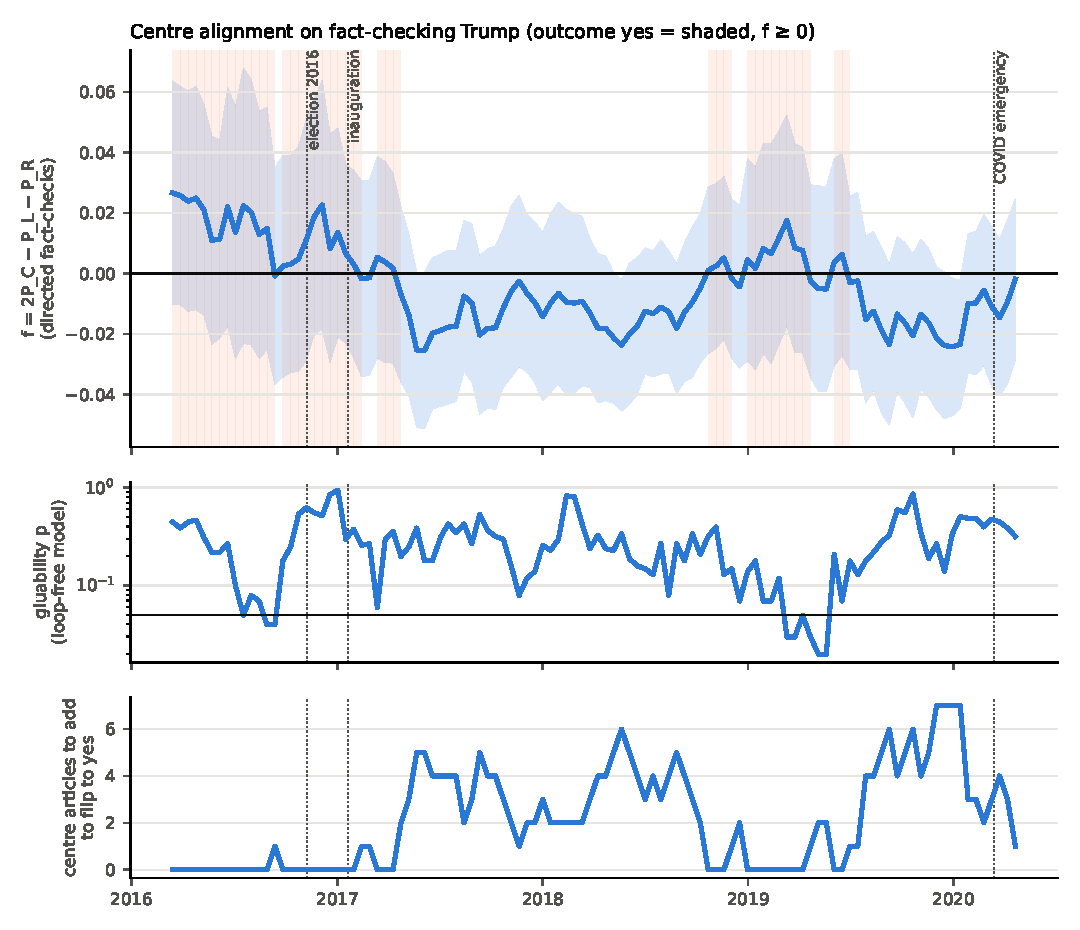
\includegraphics[width=\linewidth]{stream_outcome.pdf}
\caption{Streaming gluability-to-outcome map. Top: $f$ with 95\% band, shaded where the outcome is ``yes''. Middle: gluability $p$ of the loop-free model, with the $0.05$ line. Bottom: centre articles that would have to be added to flip ``no'' to ``yes''. Windows are 26 weeks long, plotted at their midpoint, with events as dotted lines.}\label{fig:stream}
\end{figure}

\subsection{Gluing-lattice dynamics: what jumps and what moves continuously}\label{sec:gldyn}
A natural picture ties three things together: the gluing lattice, the possibilistic class $\gamma$, and the contextual fraction CF. In that picture an ``obstructed'' region has $\mathrm{CF}>0$ and $\gamma\ne0$, a ``glueable'' region has $\mathrm{CF}=0$ and $\gamma=0$, and crossing between them is a sharp phase transition. Part of this is right.
\begin{itemize}
  \item \emph{The two layers behave differently.} Support-level (AMB) invariants jump when a support changes, while probabilities move continuously inside a face. This matches Propositions~\ref{prop:toggle} and~\ref{prop:ambtoggle}.
  \item \emph{Gluing, extension and IPF.} When the marginals of a region have a joint, the extension set is a non-empty convex polytope, and IPF from the uniform law converges to its maximum-entropy member, the I-projection \cite{csiszar}. When no joint exists, IPF does not settle.
  \item \emph{A face function and continuous entropies.} $S_0$, the log of the support size, is a face function and registers support changes. $S_\alpha$ for $\alpha>0$ varies continuously inside a face.
\end{itemize}
The three objects nevertheless come apart:
\begin{enumerate}
  \item \emph{$\gamma=0$ is not gluing.} AMB cohomology is sound but incomplete: $\gamma\ne0$ certifies contextuality, but $\gamma=0$ does not certify a global section.
  \item \emph{$\mathrm{CF}>0$ is not $\gamma\ne0$.} A full-support contextual model has $\mathrm{CF}>0$ and $\gamma=0$, because its possibilistic collapse is non-contextual. The two-box picture leaves out this whole region.
  \item \emph{Obstruction does not pin probabilities.} Marginals locked at $1/2$ is the special result for two-outcome non-flat cycles (Proposition~\ref{prop:two}), not a property of obstructed regions. In MBIC and NewsWCL50 the obstructed regions have freely varying probabilities.
  \item \emph{CF has no jump.} CF is the value of a linear program, continuous and convex in the model, and it leaves $0$ continuously at the boundary of the non-contextual polytope. The discontinuities are only in support-level quantities.
  \item \emph{The data gluing lattice is statistical.} Its verdicts come from a hypothesis test, so they depend on $N$ (Section~\ref{sec:certificate}). It computes neither CF nor $\gamma$.
\end{enumerate}
\begin{center}\small
\begin{tabular}{p{0.16\linewidth}p{0.3\linewidth}p{0.2\linewidth}p{0.2\linewidth}}
\toprule
quantity & what it measures & at a support change & inside a face\\
\midrule
$\gamma$ (AMB) & possibilistic obstruction; sound, not complete & jumps & constant\\
$S_0$ & log support size & jumps & constant\\
CF & probabilistic contextuality (LP) & continuous & continuous, piecewise linear along mixtures\\
$S_\alpha$, $\alpha>0$ & entropies & continuous & continuous\\
IPF & converges iff a joint exists ($\mathrm{CF}=0$) & -- & --\\
gluing lattice (data) & statistical fit of the loop-free model on sub-covers & depends on $N$ & depends on $N$\\
\bottomrule
\end{tabular}
\end{center}

\textbf{The path experiment} (\texttt{examples/dynamics/gluing\_lattice\_dynamics.py}, Figure~\ref{fig:gldyn}). On the CHSH scenario (a 4-cycle of contexts) take $e(\lambda)=\lambda\,\mathrm{PR}+(1-\lambda)\,\text{white noise}$. The empirical support uses a tolerance $\tau=0.02$: a cell with $p<\tau$ counts as impossible. Along $\lambda$:
\begin{itemize}
  \item \emph{CF.} CF is $0$ up to $\lambda=1/2$, then exactly linear, $\mathrm{CF}=2\lambda-1$. There is no jump.
  \item \emph{$\gamma$ and $S_0$.} Both change once, at the support collapse $\lambda=1-4\tau=0.92$. There $S_0$ falls from $\log4$ to $\log2$ and $\gamma\ne0$ switches on (strong contextuality).
  \item \emph{The stretch the two-box picture misses.} On $\lambda\in(0.5,0.92)$, $\mathrm{CF}>0$ but $\gamma=0$: the model is probabilistically contextual and possibilistically clean.
  \item \emph{IPF.} IPF converges exactly where $\mathrm{CF}=0$ (checked at every grid point). Beyond $\lambda=1/2$ its residual stays bounded away from $0$ and grows with CF.
  \item \emph{The statistical verdict.} With $N$ samples per context, a one-sided CHSH test flags the full cover as obstructed. At $\lambda=0.52$ ($\mathrm{CF}=0.04$) its power is $0.11$, $0.15$, $0.45$ and $0.93$ for $N=50$, $200$, $1000$, $5000$. It tracks CF only when $N$ is large.
  \item \emph{The lattice.} Every proper sub-cover (3 of the 4 contexts) is a tree and always glues (Theorem~\ref{thm:vorobev}), so the full cycle is the only possible minimal obstruction.
\end{itemize}
\begin{figure}[!htbp]\centering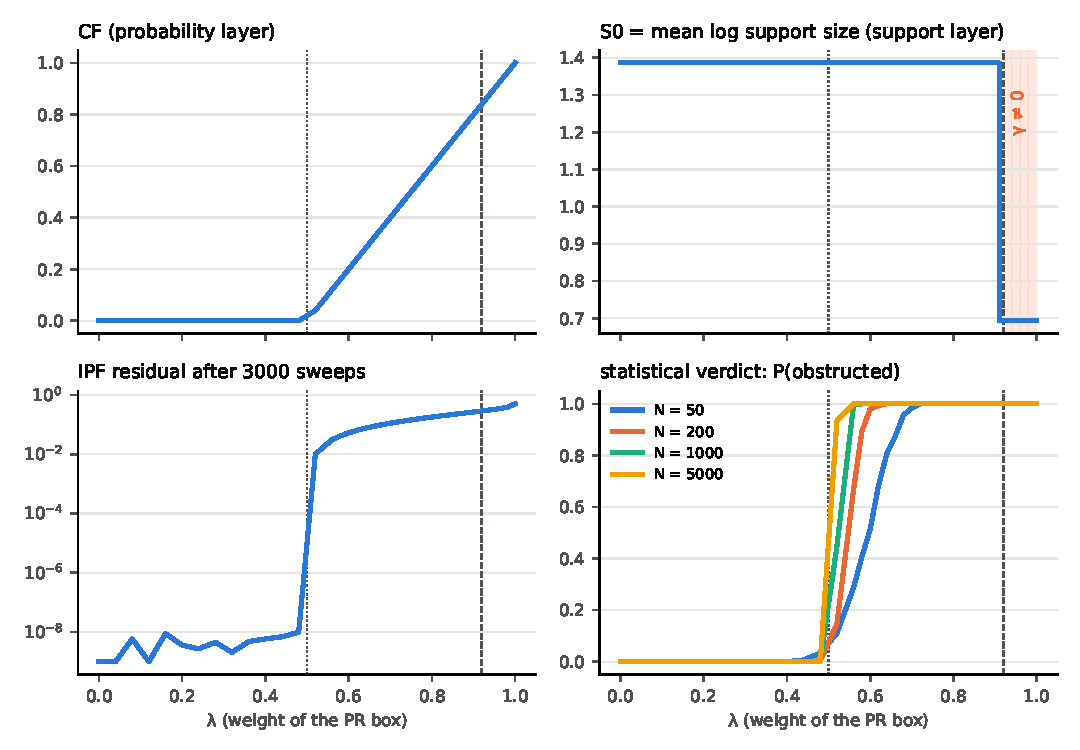
\includegraphics[width=\linewidth]{gluing_lattice_dynamics.pdf}
\caption{Along $e(\lambda)=\lambda\,\mathrm{PR}+(1-\lambda)\,$noise: CF is continuous and piecewise linear; $S_0$ and $\gamma$ jump only at the support collapse (dashed, $\lambda=0.92$, support tolerance $0.02$); IPF converges exactly where $\mathrm{CF}=0$ (dotted, $\lambda=1/2$); the statistical verdict sharpens toward the CF boundary as $N$ grows.}\label{fig:gldyn}
\end{figure}

\subsection{An outcome series, and all layers on one time axis}\label{sec:outcomeseries}
All the preceding AllSides results concern media alignment. To attach perturbations to an \emph{outcome}, we use two poll series that cover the whole coverage window (\texttt{examples/outcomes/outcome\_series.py}); neither is redistributed.
\begin{itemize}
  \item \emph{2017 to August 2020: net approval of Trump.} FiveThirtyEight's presidential approval poll list, 5{,}920 ``All polls'' polls, using their adjusted approve $-$ disapprove and poll weights (CC BY 4.0; mirrored on GitHub \cite{fte}).
  \item \emph{May 2015 to November 2016: the Trump $-$ Clinton margin.} 562 national likely- and registered-voter polls from HuffPost Pollster, as distributed with the Economist's 2020 forecast model \cite{econpolls}.
\end{itemize}
This gives 190 weekly approval points and 68 weekly margin points.

\emph{Coverage does not lead the outcome.} We correlated the week-to-week changes of coverage with those of the outcome at lags of $-8$ to $+8$ weeks. The null shifts the coverage series circularly, which keeps its autocorrelation. No lag is significant:
\begin{itemize}
  \item centre alignment $f$ against net approval: $r=-0.19$ at $+6$ weeks, max-over-lags $p=0.33$;
  \item left--right adversarial gap against net approval: $r=-0.21$ at $-7$ weeks, $p=0.25$;
  \item for the 2016 margin, $p\ge0.84$.
\end{itemize}
This agrees with the early-warning result: coverage describes, it does not anticipate.

\emph{The outcome moves at some events.} Net approval (or the 2016 margin), before versus after:
\begin{itemize}
  \item Access Hollywood tape: margin $-3.0\to-6.1$;
  \item Comey letter: margin $-5.8\to-4.4$;
  \item Charlottesville: approval $-12.1\to-16.9$;
  \item Mueller report: approval $-11.4\to-11.2$;
  \item impeachment inquiry: approval $-11.1\to-10.3$;
  \item COVID emergency: approval $-10.7\to-9.7$, a small rally.
\end{itemize}
The 2016 events compare 4 weeks before with 2 weeks after; the others compare 26 weeks either side. Charlottesville and Access Hollywood are the large moves. The approval series is strongly autocorrelated, so nominal $z$ values overstate the evidence. Charlottesville is a clean case of the \emph{outcome moving while the coverage layers do not}: it showed no non-natural change and no step (Section~\ref{sec:slepian}).

\textbf{All layers on one axis} (\texttt{examples/outcomes/layers\_chart.py}, Figure~\ref{fig:layers}). For 26-week windows stepped every 2 weeks, the figure stacks six panels:
\begin{enumerate}
  \item the outcome;
  \item the probability layer ($P_L$, $P_C$, $P_R$);
  \item the perturbation relative to 26 weeks earlier, split by Proposition~\ref{prop:natural} into its natural (re-calibration) and non-natural (loop) parts;
  \item contextuality on the \emph{triangle scenario}, detailed below;
  \item the gluing defect, the KL distance to the nearest consistent global law;
  \item gluability.
\end{enumerate}
The triangle scenario has measurements L, C, R $\in\{$adversarial, not$\}$ and contexts $\{L,C\}$, $\{C,R\}$, $\{L,R\}$. The table of each context counts the stories covered by both sides. Different stories feed different contexts, so the family can fail to glue: by the single-source theorem, only different units can.
\begin{itemize}
  \item \emph{$\gamma=0$ in all 95 windows}, because the support is full. CF ranges over $0.01$--$0.10$. \emph{The data sit in the region the two-box picture leaves out} (Section~\ref{sec:gldyn}): probabilistically non-glueable, possibilistically clean.
  \item \emph{CF here is mostly signalling.} CF is highly correlated with the between-context disagreement of each side's marginal ($r=0.85$), which arises because different stories feed different pairs. It is a gluing defect of the cover, not Bell-type contextuality.
  \item \emph{CF and the gluing defect peak in mid-2019, after the Mueller report.} This is the same period in which the naturality test found the only non-natural change (Section~\ref{sec:slepian}).
  \item \emph{Natural and non-natural perturbations are of similar size} (median RMS $0.061$ and $0.054$ per cell over 26 weeks).
  \item \emph{The window-level layers correlate weakly with mean approval}: $r=+0.33$ for CF, $+0.26$ for the natural part, $+0.21$ for the non-natural part, $+0.09$ for gluability $p$. The 87 overlapping windows amount to about 7 independent ones, so none of this is significant.
\end{itemize}
\begin{figure}[!htbp]\centering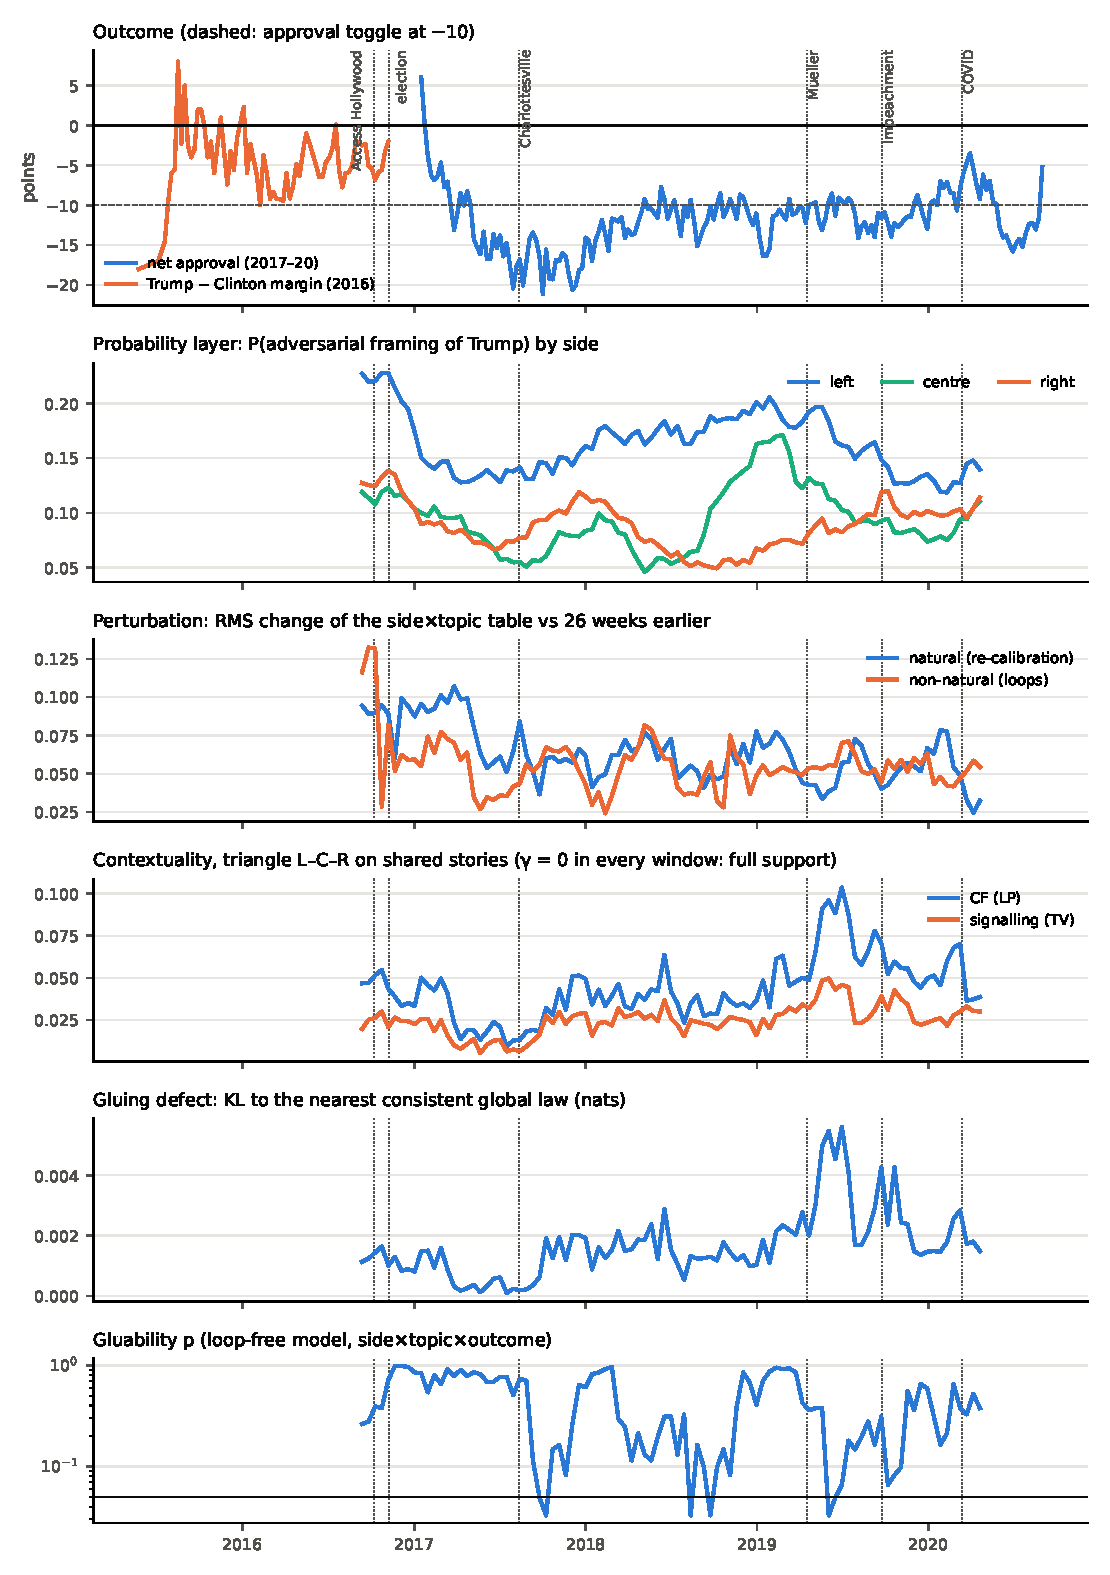
\includegraphics[width=\linewidth]{layers_chart.pdf}
\caption{All layers on one time axis (AllSides coverage of Trump, with the approval and 2016-margin outcome). Panels: outcome; the three sides' probability of adversarial framing; perturbation relative to 26 weeks earlier, natural against non-natural; contextuality on the L--C--R triangle over shared stories (CF and signalling; $\gamma=0$ throughout); gluing defect; gluability. Events are dotted.}\label{fig:layers}
\end{figure}

\subsection{Paths over the gluing lattice: raising the probability of an outcome}\label{sec:latticepath}
Can one raise the probability of an outcome by gluing the right regions? Take a binary label on source $\times$ topic cells, and a \emph{region}, meaning a set of topics. On a region the glued (loop-free) model is additive in log-odds, $\operatorname{logit}p(s,t)=\alpha_s+\beta_t$, fitted in closed form by weighted least squares. The region glues if its weighted loop residual passes $\chi^2$. A held-out target cell $(s^*,t^*)$ is predicted by $\hat p=\operatorname{expit}(\alpha_{s^*}+\beta_{t^*})$, and the outcome is $[\hat p>1/2]$. A \emph{path} is a chain of glueable regions along which $\hat p$ rises, or falls (\texttt{amb\_vigneaux/lattice\_path.py}).

\begin{proposition}[Region dependence is loop content]\label{prop:regioninv}\st{proved; checked}
If the true log-odds are additive (no loops), every region that contains $t^*$ and the source $s^*$ gives the same prediction, up to sampling noise. The spread of $\hat p$ across glueable regions is therefore produced only by loops and noise. A path that raises $\hat p$ moves the estimate along the loop part of the data, not along anything the loop-free model says about the target.
\end{proposition}
\begin{proof}
With additive truth the weighted least-squares fit on any such region recovers $\alpha_{s^*}+\beta_{t^*}$ exactly in the noiseless limit, because the design is identified on the region. Differences between regions come from residuals, which are loops plus noise. It is checked in \texttt{tests/test\_lattice\_path.py}: the spread is below $10^{-3}$ for additive data, and positive with planted loops.
\end{proof}

\textbf{MBIC} (\texttt{examples/lattice\_path/mbic\_paths.py}; 82 held-out outlet $\times$ topic cells; glueable regions of 5--7 topics containing $t^*$, about 5{,}000 per target):
\begin{itemize}
  \item \emph{Paths exist and are long.} For HuffPost $\times$ sport (true share $0.65$), dropping topics from the full cover raises $\hat p$ from $0.60$ to $0.94$ in nine glueable steps, and a different sequence lowers it to $0.35$. The median width of the envelope $[\min\hat p,\max\hat p]$ is $0.34$.
  \item \emph{The binary outcome can be flipped by region choice for 36 of 82 targets (44\%).} The held-out truth lies inside the envelope for 53 of 82.
  \item \emph{Choosing regions for the desired outcome is cherry-picking.} Mean absolute error against the held-out truth is $0.112$ for the full cover, $0.112$ for the median over glueable regions and $0.112$ for the glue-$p$-weighted average. It rises to $0.172$ at the end of the raise path and $0.185$ at the end of the lower path, 55--65\% worse.
  \item \emph{Small regions are the danger.} Regions of 2 topics always pass the glue test, because such a test has no power, and they spread $\hat p$ over $0.05$--$0.9$. A minimum region size is essential.
\end{itemize}

\textbf{When gluing the right regions helps} (\texttt{examples/lattice\_path/synthetic\_paths.py}). We use 8 sources $\times$ 12 topics with additive log-odds, plus loops planted in 3 contaminated topics, 30 units per cell, and targets in clean topics, over 640 cases. The full cover never glues.
\begin{itemize}
  \item Pruning by \emph{consistency}, dropping the topic whose removal most improves the glue $p$ until the region glues, reduces the error from $0.045$ (full cover) to $0.039$, 13\% better.
  \item Pruning toward a \emph{desired outcome} increases it to $0.073$ (raise) and $0.078$ (lower).
\end{itemize}

\textbf{Feedback, and paths versus surfaces} (\texttt{examples/lattice\_path/landscape.py}). Suppose a step that raised $\hat p$ is taken as evidence that nearby regions also raise it (and a step that lowered it as a reason to move away). This feedback is justified exactly when the landscape $\eta(U)=\operatorname{logit}\hat p(U)$ has low-order structure on the lattice. For 12 MBIC targets we evaluated every glueable region of at least 5 topics containing $t^*$ (7{,}000--7{,}800 regions each).

\begin{proposition}[The landscape is first order, with the loop residuals as its slopes]\label{prop:landscape}\st{proved to first order; checked}
To first order in the leverages, $\eta(U)\approx c+\sum_{x\in U}w_x$. The influence $w_x$ of topic $x$ is proportional to the weighted loop residual of the target's source on $x$ in the full fit, $w_{s^*x}\bigl(y_{s^*x}-\hat\alpha_{s^*}-\hat\beta_x\bigr)$. The region that maximises $\hat p$ is, to this order, obtained by keeping the topics where the target source sits above its additive fit and dropping those where it sits below. Every walk that moves along these signs raises $\hat p$ until the second-order terms, the shared estimation of the other effects, bend it.
\end{proposition}
\begin{proof}[Sketch]
Removing the block of cells of topic $x$ changes the weighted least-squares estimate by $-(X^\top WX)^{-1}X_x^\top W_xr_x+O(h^2)$ (the block version of Sherman--Morrison, i.e.\ DFBETA). Its component along $\alpha_{s^*}+\beta_{t^*}$ is proportional to the source-$s^*$ residual on $x$ when the design is balanced, and the effects of removing several blocks add at first order. It is checked in \texttt{tests/test\_lattice\_path.py} ($R^2>0.8$ and correlation $>0.8$ on a synthetic grid).
\end{proof}
\noindent On the 12 MBIC targets:
\begin{itemize}
  \item \emph{The landscape is first order.} Per-topic influences explain a median $R^2=0.89$ of $\eta$ over the lattice, and adding pairwise terms explains $0.98$.
  \item \emph{The slopes are the loop residuals.} The fitted influences correlate $0.86$--$0.99$ (median $0.97$) with the weighted loop residuals of the target outlet on each topic.
  \item \emph{Surfaces, not only paths.} We call a move \emph{aligned} if it adds a topic with positive influence or drops one with negative influence. Aligned moves raise $\hat p$ in a median $86\%$ of cases. The ascending set is an \emph{interval of the lattice}: keep the raisers, drop the lowerers. Almost any walk inside it climbs, so it is a surface rather than a single path. It is not a variety in the algebraic sense, but a nearly linear set function on the Boolean lattice.
  \item \emph{Feedback works, up to local optima.} Hill-climbing that accepts only raising steps reaches the global maximum from $59\%$ of random starts, in about 6 steps. The failures are the pairwise terms, which create local optima, so feedback with a few restarts is enough.
\end{itemize}
\noindent The feedback rule (``a step that helped points to neighbours that help'') therefore has a precise meaning: the sign of a topic's influence is stable across the lattice, because it is the sign of the target source's loop residual on that topic. The surface it climbs is the \emph{loop content} of the target source (Proposition~\ref{prop:regioninv}). Climbing it selects the topics where the source happens to be more biased than its additive fit. As a \emph{diagnostic} this is valuable, because it names the topics carrying the source-specific interaction that bears on the target. As a \emph{procedure} for raising the probability of an outcome it is evidence selection, and the accuracy costs above apply.

\textbf{How gluing lifts the probability: one target} (\texttt{examples/lattice\_path/surface\_chart.py}, Figure~\ref{fig:surface}). For Breitbart $\times$ gender (held-out share $0.67$, $n=43$) the full cover predicts $0.53$. Figure~\ref{fig:surface} shows the mechanism in three panels.
\begin{enumerate}
  \item[(a)] Each topic's influence on the prediction (bars) coincides with the outlet's loop residual on that topic (dots; correlation $0.98$). Coronavirus, sport and gun control pull $\hat p$ up. Vaccines, student debt and international politics pull it down.
  \item[(b)] Over all 7{,}691 glueable regions, $\hat p$ is almost a function of the first-order loop-content score $\sum_{x\in U}w_x$ ($R^2=0.94$). This is the surface. The raise and lower paths run along its two edges, bending where second-order terms act.
  \item[(c)] Un-gluing vaccines, student debt and international politics first lifts $\hat p$ from $0.53$ to $0.72$. The mirror path lowers it to $0.32$, across the $1/2$ line.
\end{enumerate}
In this target the raise path passes the held-out truth, but that is luck, not method. Over all 82 targets, outcome-driven paths are 55--65\% worse than the full cover. What the figure explains is \emph{why} gluing moves the probability: each glued region adds or removes a slice of the target outlet's loop content.

\begin{figure}[!htbp]\centering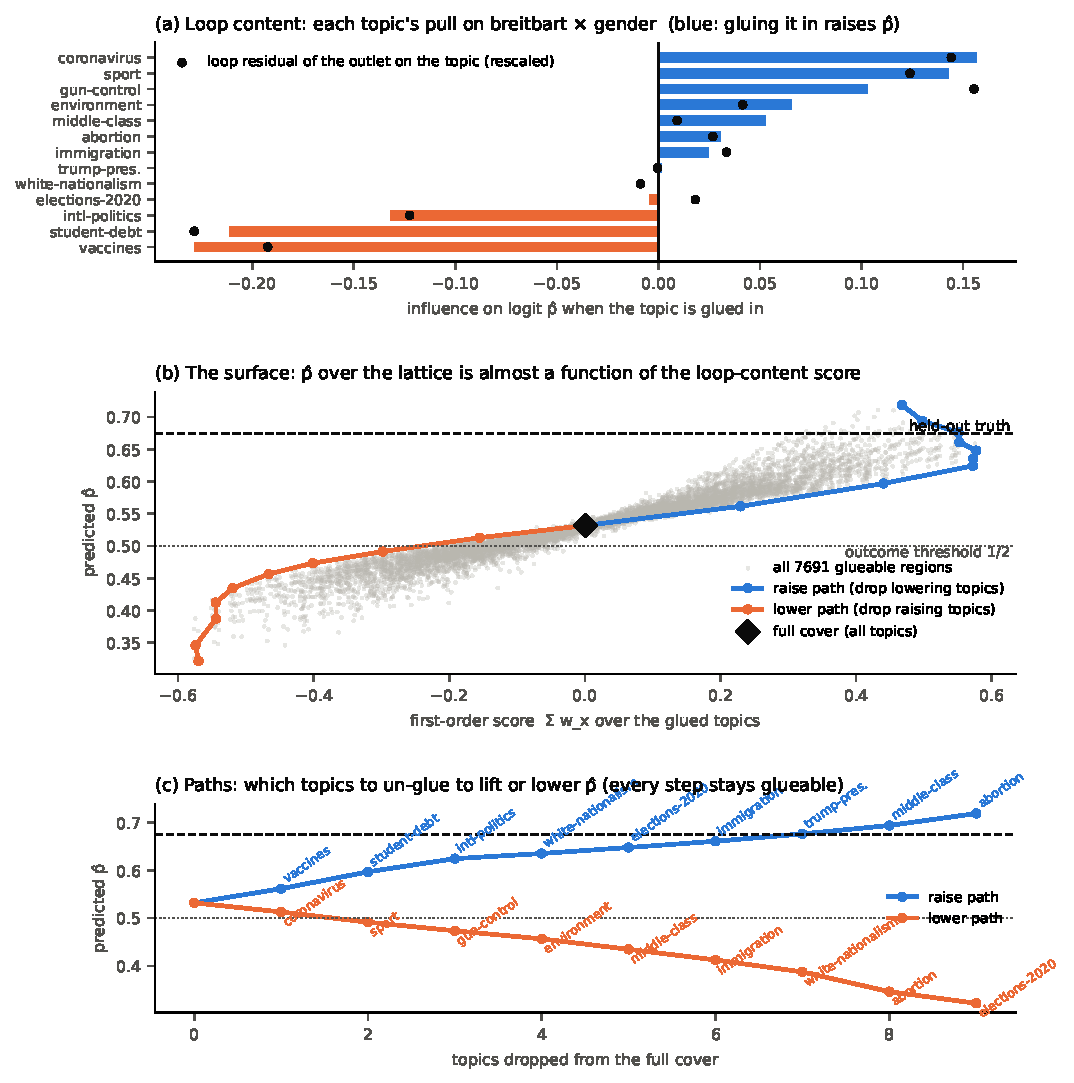
\includegraphics[width=\linewidth]{surface_chart.pdf}
\caption{How gluing regions lifts or lowers a predicted probability (MBIC, Breitbart $\times$ gender held out). (a) Loop content: each topic's first-order influence on $\operatorname{logit}\hat p$ when glued in (bars), against the outlet's weighted loop residual on the topic (dots, rescaled). (b) The surface: every glueable region placed by its loop-content score against its $\hat p$, with the raise and lower paths, the full cover, the held-out truth (dashed) and the outcome threshold (dotted). (c) The paths step by step, labelled by the topic un-glued; every step stays glueable. In this target the raise path happens to reach the truth; over 82 targets such paths are 55--65\% less accurate than the full cover.}\label{fig:surface}
\end{figure}

\textbf{Relation to the literature.} The negative result is not a new phenomenon.
\begin{itemize}
  \item \emph{Selection bias.} Choosing a region by how it moves the prediction is selection on the outcome. The end of a raise path is the maximum over thousands of noisy estimates (about 5{,}000 regions per target), so it suffers the winner's curse. The standard remedies are data splitting \cite{cox75} and selective inference \cite{posi,fithian}, and the bias of model selection evaluated on the same data is well documented \cite{varma06,cawley10}. Our leave-one-cell-out design is what exposes it.
  \item \emph{Small regions.} The danger of low-power selection among many candidates is the standard overfitting-in-model-selection result \cite{cawley10}.
  \item \emph{The form of the bias.} The first-order form of Proposition~\ref{prop:landscape}, where un-gluing a block shifts the estimate by its weighted residual, is the block version of the classical influence diagnostics DFBETA and Cook's distance \cite{cook77,bkw80}.
  \item \emph{The consistency path} is direction-blind, since it drops the worst-fitting topics whichever way they push. It therefore adds no directional bias to point predictions. It still selects on the same data, so standard errors reported after pruning are too small, and honest intervals need data splitting or selective inference \cite{cox75,fithian}. This section reports point errors only.
\end{itemize}
What is specific to this paper is narrower. It identifies these influence blocks with the loop ($H^1$) coordinates of the gluing complex, and draws two consequences:
\begin{itemize}
  \item the spread of predictions across regions is exactly the loop content bearing on the target (Proposition~\ref{prop:regioninv});
  \item the ascending set is an interval of the lattice, so feedback search is justified by the stability of the residual signs (Proposition~\ref{prop:landscape}).
\end{itemize}
This translates standard influence diagnostics into the language of gluing, which is what connects region choice to the rest of the paper. It is not a new statistical phenomenon.

\noindent\emph{Conclusion.} The lattice supports both kinds of path, and they must not be confused.
\begin{itemize}
  \item A \emph{consistency path} (glue the regions that fit together, drop the obstructed ones) is estimation. It improves prediction when some regions are contaminated.
  \item An \emph{outcome path} (glue the regions that push $\hat p$ where one wants it) is selection on the loop part. It can flip the conclusion for almost half the targets and it degrades accuracy.
  \item The honest report of ``raising the probability by gluing'' is therefore the envelope together with the consistency path. The envelope's width is the sensitivity of the conclusion to the choice of regions, and by Proposition~\ref{prop:regioninv} it measures the loop content that bears on the target.
  \item A \emph{real} rise in the outcome's probability needs a change in the world: a perturbation of the data, with the costs of Propositions~\ref{prop:toggle} and~\ref{prop:ambtoggle}. It cannot come from a change in which data are glued.
\end{itemize}

\subsection{Hull covers on the lattice: discs without direction}\label{sec:hullcover}
The outcome paths above select on the outcome. A proposed direction-blind alternative is to let a hull choose the regions. Build the Berkovich hull of the cell values (for arithmetic data) or the single-linkage dendrogram (for rates); its discs at radius $r$ form a cover. Take the largest radius whose discs glue as the canonical region, and read the spread of predictions along the radius as a canonical sensitivity report. The radius is a scale, not an outcome, so the choice is direction-blind. We tested this on every corpus (\texttt{examples/lattice\_path/hull\_experiment.py}, \texttt{tests/test\_hull\_direction.py}).

\textbf{Construction.} Each cell $(s,t)$ with at least $10$ units is held out in turn. Every feature is computed without it. The topics are clustered by single linkage with the Euclidean metric. Its merge heights form an ultrametric, so the discs of one radius partition the topics. We used three features per topic:
\begin{itemize}
  \item \emph{value}: the pooled rate (one number);
  \item \emph{profile}: the column of empirical logits over sources;
  \item \emph{loop}: the column of weighted loop residuals $\sqrt{w}\,(y-a_s-b_t)$ of the full-cover additive fit, i.e.\ the Hodge loop part.
\end{itemize}
Along the chain of discs containing the target topic, the canonical region is the largest disc with at least $m$ topics that glues ($\chi^2$ loop test, as in Section~\ref{sec:latticepath}); if none glues, it is the smallest disc with at least $m$ topics. We take $m=5$ on MBIC and $m=2$ elsewhere, since a region must contain another topic of the target's source. The p-adic hull does not apply: the data are rates, and the p-adic distance on them is arbitrary (Section~\ref{sec:hull}).

\begin{table}[!htbp]\centering\small
\caption{Hull covers against the full cover and against models of the loop (mean $|\hat p-\text{truth}|$ over held-out cells). ``Sub'' is the number of targets for which the hull chose a proper sub-region. ``Chain'' is the median spread of $\hat p$ along the hull's discs, and ``lattice'' the median spread over all glueable regions. The oracle picks the best glueable region using the truth. The last two model columns fit the loop: rank-1 interaction $a_s+b_t+u_sv_t$, and tropical rank~2 ($\min$ or $\max$ of two additive regimes, i.e.\ columns on a tropical line, which is a tree). Both are fitted by alternating closed-form weighted least squares. In brackets: the number of targets beaten against the full cover.}\label{tab:hullcover}
\resizebox{\linewidth}{!}{\begin{tabular}{lcccccccccc}
\toprule
corpus ($S\times T$, targets) & full glues & full & hull & sub & chain & lattice & oracle & rank-1 & trop.\ min & trop.\ max\\
\midrule
MBIC ($8\times14$, 82) & 82 & .112 & .112 & 0 & .02--.06 & .336 & .021 & .150 (33) & .177 (23) & .129 (35)\\
NewsWCL50 ($5\times5$, 23) & 15 & .128 & .138--.139 & 8 & .03--.07 & .230 & .056 & .076 (16) & .090 (16) & .238 (4)\\
AllSides adv.\ ($3\times9$, 27) & 27 & .020 & .020 & 0 & .005--.010 & .082 & .005 & .077 (4) & .036 (10) & .110 (5)\\
AllSides dir.\ ($3\times9$, 27) & 27 & .006 & .006 & 0 & .002--.003 & .024 & .002 & .016 (14) & .007 (13) & .050 (2)\\
BASIL ($3\times2$, 6) & 4 & .087 & .087 & 0 & 0 & -- & -- & .097 (1) & .112 (2) & .237 (0)\\
\bottomrule
\end{tabular}}
\end{table}

\textbf{Findings} (Table~\ref{tab:hullcover}).
\begin{itemize}
  \item \emph{The hull chooses nothing where the corpus glues.} On MBIC and AllSides the root disc glues, so under every feature the canonical region is the full cover. BASIL has only two topics: dropping either one isolates the target's source, so there is nothing to choose.
  \item \emph{Where the corpus tears, the hull does not help.} On NewsWCL50 the full cover fails for 8 of 23 held-out cells. For exactly those cells the hull chose a sub-region, and the error rose slightly ($0.138$ against $0.128$; noise at $n=8$).
  \item \emph{As a sensitivity report the chain is misleading.} Its spread is $\tfrac14$ to $\tfrac16$ of the spread over all glueable regions, so reporting it would understate the dependence on region choice several-fold.
  \item \emph{Better regions exist, but no target-blind metric stitches them.} The oracle reaches $0.021$ (MBIC) and $0.056$ (NewsWCL50), but it chooses with the answer. The one target-blind signal is how the \emph{other} sources' loops co-vary across topics. A region stitched from the topics positively correlated with the target topic on that signal did worse than the full cover ($0.130$ MBIC, $0.141$ NewsWCL50; not computable with three sources).
  \item \emph{The information is in the loop pattern, and it is used by modelling the loop, not by choosing regions.} On the one corpus that tears (NewsWCL50) both loop models beat the full cover ($0.076$ and $0.090$ against $0.128$, 16 of 23 targets, sign test $p=0.09$). Where the corpus glues, the loops are noise and the additive full cover is best. The switch has to be made per corpus, by the robustness certificate. It cannot be made per cell: the cells whose removal leaves the rest gluing are the ones carrying the loop. This result is suggestive and needs a second corpus that tears.
\end{itemize}

\begin{proposition}[Hulls are blind to direction]\label{prop:hulldirection}\st{proved; checked}
Relabel the outcome, $k\mapsto n-k$ in every cell. Then:
\begin{enumerate}
  \item the empirical logits change sign, $y\mapsto-y$, so every value, profile and loop feature above changes sign (or, for rates, $r\mapsto1-r$);
  \item every hull distance (Euclidean, ultrametric, or $p$-adic, since $|{-x}|_p=|x|_p$), and hence every disc, merge height, radius profile and gluing verdict, is unchanged;
  \item the signed loop residual of the target source on each topic, which is the first-order influence of that topic on $\operatorname{logit}\hat p$ (Proposition~\ref{prop:landscape}), changes sign.
\end{enumerate}
So a hull, the AMB class $\gamma$ (valued in a group without order) and $\CF$ (a distance) can say \emph{whether} and \emph{at what scale} an outcome is fragile, but never \emph{which way} it tips. Direction needs ordered (real) coefficients and a target functional: the signed Hodge loop part on the lattice, and the probabilities it moves.
\end{proposition}
\begin{proof}
(1) The smoothed logit satisfies $\operatorname{logit}\frac{n-k+1/2}{n+1}=-\operatorname{logit}\frac{k+1/2}{n+1}$, and the weights $n\,p(1-p)$ are unchanged. The additive fit is linear in $y$, so its coefficients and residuals change sign. (2) Every distance used is a norm or an absolute value, and $\|{-v}\|=\|v\|$. The $\chi^2$ loop statistic is quadratic in the residuals. (3) This is (1) applied to the target row. Checked on all five corpora: the hull chains and merge heights are identical in all $495$ (target, feature) cases, and the target's loop residuals flip sign in $165/165$ targets. \texttt{tests/test\_hull\_direction.py} checks the same on a synthetic table.
\end{proof}
\noindent The tropical columns of Table~\ref{tab:hullcover} show the same thing from the model side. The tree-shaped model (a tropical line) needs a choice of $\min$ or $\max$. Relabelling swaps them, and the better choice differs by corpus ($\min$ on NewsWCL50, $\max$ on MBIC). The discs of a hull may locate where gluing fails and at what scale, but they do not carry the dimension along which a favourable outcome is favourable. For that the engine needs the lattice and the probabilities.

\subsection{Bounds on an outcome over all gluings}\label{sec:bounds}
The lattice envelope ranges over choices of \emph{region}. The adjunction of Proposition~\ref{prop:kerneladj} gives the complementary range: over \emph{global laws}, with the cover held fixed. Let $R:\mathcal D(E(X))\to\mathrm{Fam}(\mathcal U)$ be restriction. For a family $e$, the preimage $R^\ast e=R^{-1}(e)$ is the polytope of global laws consistent with every local table. For an outcome $f$ on global sections (an event that may involve measurements never observed together, or any real score), put
\[ \mathrm{lo}(f)=\min_{P\in R^{-1}(e)}\langle f,P\rangle,\qquad \mathrm{hi}(f)=\max_{P\in R^{-1}(e)}\langle f,P\rangle, \]
two linear programmes (\texttt{amb\_vigneaux/bounds.py}, \texttt{examples/bounds/run.py}, \texttt{tests/test\_bounds.py}). In statistics these are partial-identification (Fr\'echet) bounds \cite{frechet51,manski03}. What the gluing language adds is where the width comes from, and what an empty preimage means.

\begin{proposition}[Bounds over all gluings]\label{prop:bounds}\st{proved; checked}
\leavevmode
\begin{enumerate}
  \item \emph{Order, not a lever.} Relabelling the outcome maps $[\mathrm{lo},\mathrm{hi}]$ to $[1-\mathrm{hi},1-\mathrm{lo}]$. So the interval is ordered, unlike $\gamma$, $\CF$ and every hull quantity (Proposition~\ref{prop:hulldirection}). It says how far the data pin the outcome down, not what would move it or which way: the levers are the signed loop influences on the lattice (Proposition~\ref{prop:landscape}).
  \item \emph{No selection.} The interval ranges over every gluing, so there is nothing to cherry-pick. The maximum-entropy member (IPF) is a point inside it.
  \item \emph{Width is loop content.} The preimage is $P_0+\ker R$ intersected with the simplex. So $f$ is \emph{identified} (width $0$ for every $e$) iff $f\perp\ker R$ modulo constants, and otherwise the width is set by the component of $f$ along $\ker R$. On the triangle cover $\{L,C\},\{C,R\},\{L,R\}$ with binary outcomes, $\ker R$ is spanned by the three-way parity $\chi=(-1)^{L+C+R}$. Unanimity $P(L=C=R)$ has $\langle f,\chi\rangle=0$ and is identified: indeed $P(\text{not unanimous})=\tfrac12\sum_{\text{pairs}}P(x_i\ne x_j)$. ``All three'' ($\langle f,\chi\rangle=-1$) and ``majority'' ($+2$) are not.
  \item \emph{Empty preimage is the counit failure.} $R^{-1}(e)=\emptyset$ iff $e$ is contextual or signalling. Then two honest fallbacks are reported together with the size of the failure: the preimage of the nearest consistent family $R(q^\ast)$, with its gluing defect; or the normalised non-contextual parts of mass $1-\CF$, with $\CF$.
  \item \emph{The CHSH chain.} For $e_\lambda=\lambda\,\mathrm{PR}+(1-\lambda)\,\mathrm{noise}$, bounding the correlator of the closing context from the other three gives $[\max(-1,3\lambda-2),\,1]$. Its truth, $-\lambda$, lies inside iff $\lambda\le\tfrac12$, i.e.\ iff $\CF=0$: the held-out bound \emph{is} the CHSH inequality. The maximum-entropy point $\lambda^3$ (Proposition~\ref{prop:condprod}) lies inside the interval but is far from the truth.
\end{enumerate}
\end{proposition}
\begin{proof}
(1) The relabelling permutes global sections and sends $f$ to $1-f$ on the relabelled law, so the two programmes exchange. (2) The preimage contains every global law consistent with $e$, and IPF converges to one of them when the preimage is non-empty \cite{csiszar}. (3) $\langle f,P_0+v\rangle$ is constant on the preimage iff $\langle f,v\rangle=0$ for every feasible direction $v\in\ker R$. For the triangle, $R$ has rank $7$ on $\mathbb R^8$, and $R\chi=0$ because $\chi$ sums to zero over every pair-marginal fibre. The unanimity identity is the count that a non-constant triple disagrees on exactly two of its three pairs. (4) is Proposition~\ref{prop:kerneladj}(1). (5) Along the chain the three link correlators are $\lambda$, and the extreme points of the preimage give the closing correlator $\ge\lambda+\lambda+\lambda-2$, which is the CHSH bound. Checked exactly for $11$ values of $\lambda$ in the tests.
\end{proof}

\textbf{Validation on real triangles.} We use units on which all three of $L,C,R$ are observed, so the truth of every functional is known. Each context's table is taken from its own disjoint quarter of the units, and the truth from the fourth quarter (200 random splits). Coverage is reported for three intervals:
\begin{itemize}
  \item the plug-in bounds;
  \item the bounds widened by a bootstrap of each quarter ($2.5\%$ of lo, $97.5\%$ of hi);
  \item the bootstrap bounds also widened by the sampling error of the fourth-quarter truth.
\end{itemize}
The sample tables signal slightly, so the preimage is empty in almost every split and the projected fallback is used. The units are:
\begin{itemize}
  \item MBIC: annotator groups by political ideology, each group's outcome the group majority on a sentence ($1{,}600$ sentences);
  \item AllSides: sides on a story, outcome ``any adversarial article'' ($736$ stories covered by all three).
\end{itemize}
\begin{center}\small
\resizebox{\linewidth}{!}{\begin{tabular}{llcccc}
\toprule
corpus & outcome & width (plug-in / boot.) & coverage plug-in & boot. & boot.\,+\,truth noise\\
\midrule
MBIC & all three biased & .117 / .176 & .90 & .97 & 1.00\\
 & majority & .235 / .289 & 1.00 & 1.00 & 1.00\\
 & unanimous (identified) & 0 / .068 & .00 & .68 & .98\\
 & $P(L{=}R{=}1)$, $\{L,R\}$ held out & .263 / .340 & 1.00 & 1.00 & 1.00\\
AllSides & all three adversarial & .042 / .057 & .88 & .98 & 1.00\\
 & majority & .085 / .150 & .83 & .97 & 1.00\\
 & unanimous (identified) & 0 / .096 & .00 & .68 & .98\\
 & $P(L{=}R{=}1)$, $\{L,R\}$ held out & .135 / .170 & .99 & 1.00 & 1.00\\
\bottomrule
\end{tabular}}
\end{center}
\begin{itemize}
  \item Bootstrap-widened bounds cover at $0.97$--$1.00$ for every non-identified outcome.
  \item The identified outcome has width $0$. So its plug-in ``interval'' is a point estimate, and its coverage is a matter of sampling error, restored to $0.98$ once that is included.
  \item The maximum-entropy point is close in every case (mean error $0.012$--$0.049$), but it is one gluing among many. The interval says how far the data, and not the choice of gluing, pins the outcome down.
\end{itemize}
In AllSides there is also a natural design. The pair tables come from stories covered by \emph{exactly} that pair ($566$, $612$, $607$), which are disjoint by construction, and the truth from the $736$ triple stories.
\begin{itemize}
  \item The bounds contain the triple-story value for ``all three'' ($[0,.028]\ni.023$), ``majority'' ($[.052,.108]\ni.105$) and the held-out pair ($[0,.084]\ni.052$).
  \item They miss the identified unanimity ($.670$ against $.626$). Triple-covered stories are a different population, and an identified outcome has no width to absorb the shift.
\end{itemize}

\begin{figure}[!htbp]\centering
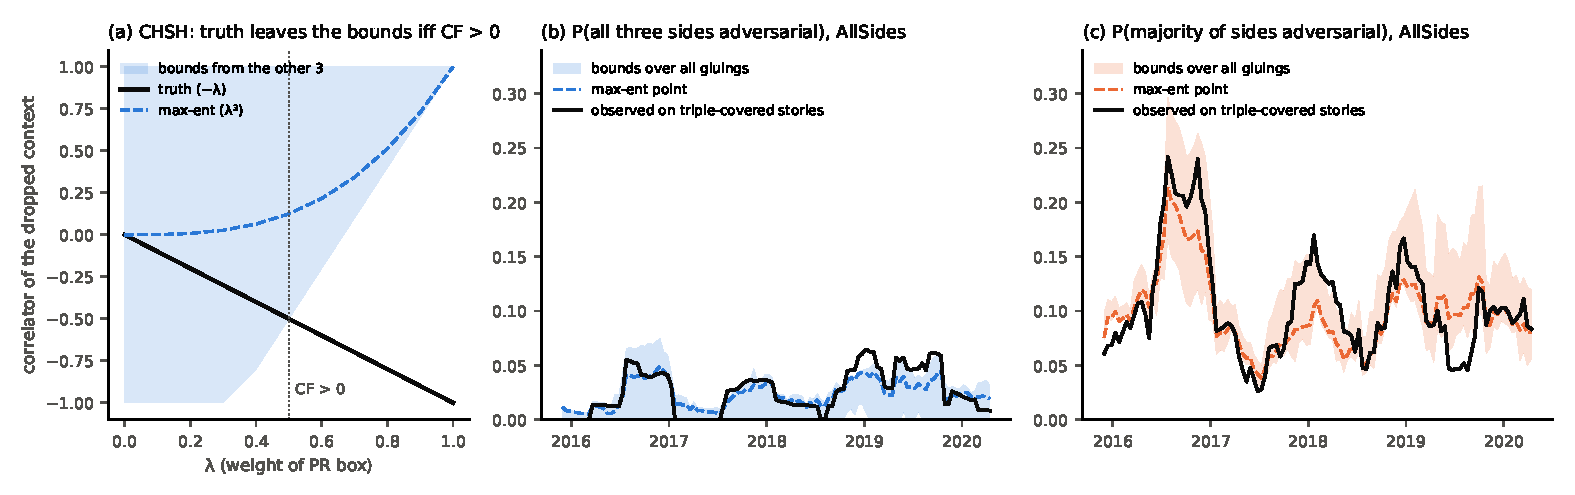
\includegraphics[width=\linewidth]{bounds_chart.pdf}
\caption{Bounds over all gluings. (a) CHSH chain: the bound on the dropped context's correlator from the other three. The truth leaves the bound exactly when $\CF>0$. The maximum-entropy point ($\lambda^3$) stays inside but far from the truth. (b, c) AllSides stream (26-week windows, step 2 weeks): bounds on $P$(all three sides adversarial) and $P$(majority adversarial) from the three pair tables (all stories covered by each pair), with the max-ent point and the value observed on stories covered by all three sides. Plug-in bounds, no sampling widening.}\label{fig:bounds}
\end{figure}

\textbf{The stream} (Figure~\ref{fig:bounds}b,c; 115 windows). The plug-in bounds are narrow:
\begin{itemize}
  \item median width $0.030$ for ``all three'' and $0.059$ for ``majority'';
  \item they contain the observed triple value in $75\%$ and $70\%$ of windows. The misses are where the triple-covered stories differ from the pair-covered ones, as in the natural design.
\end{itemize}

\textbf{The population assumption, and a test for it.} The bounds are valid for the population whose marginals the local tables estimate. Every local table must therefore sample the \emph{same} population as the target. Signalling between tables detects some violations, which is the source of the gluing defect $0.024$ above. It cannot detect a shift that only affects units seen by all three measurements, because no local table contains those units. When the populations differ the bounds can miss, and a fully identified outcome (zero width) has nothing to absorb the shift. The test is to compare, for each pair, the pair's table from pair-only units with the same pair's table from the triple-covered units. On AllSides (\texttt{examples/grey/run.py}, part 4):
\begin{itemize}
  \item $L$--$R$: TV $0.014$, $\chi^2$ $p=0.94$;
  \item $L$--$C$: TV $0.031$, $p=0.53$;
  \item $C$--$R$: TV $0.097$, $p=2\times10^{-4}$. On triple-covered stories the centre is adversarial at $0.174$ against $0.101$, and the right at $0.130$ against $0.080$.
\end{itemize}
The shift is real and located in the centre--right pair. It accounts for the unanimity miss and for the stream windows where the observed triple value falls outside the bounds. A report should run this test before quoting the bounds, and state the shift when it fails.

\textbf{How the bounds sit with the other tools.} An outcome report now has three parts:
\begin{itemize}
  \item the gluing radius, $\gamma$ and $\CF$: whether and at what scale the outcome is fragile (no direction);
  \item the lattice envelope with the signed loop influences: which regions push the outcome which way (direction, over regions);
  \item the bounds over all gluings: how far the data pin the outcome down for a fixed cover (ordered, over global laws, no selection; not a lever), and an empty preimage when the counit fails. They hold for the population the tables sample, so they come with the population test above.
\end{itemize}

\subsection{Grey contexts: what-if filters}\label{sec:grey}
A \emph{grey} context is a filter that is never observed together with the outcome. For example, ``annotators aged $55$ or over'' does not appear jointly with the bias label, but its distribution over shared covariates is known from elsewhere (a census, a panel). We may also want to ask what follows from a hypothesis about the filter. The grey context enters the cover in one of two ways, each a set of linear constraints on the global law:
\begin{itemize}
  \item \emph{population}: a known table on some variables, such as the filter's distribution within each covariate stratum. It is entered as equalities, exactly like an observed context.
  \item \emph{hypothesis}: a range for a conditional probability, $a\le P(E\mid G)\le b$. This is $P(E,G)-a\,P(G)\ge0$ and $P(E,G)-b\,P(G)\le0$, linear in $P$.
\end{itemize}
The same programmes as in Section~\ref{sec:bounds} then give three answers (\texttt{bounds.grey\_bounds}, \texttt{examples/grey/run.py}, \texttt{tests/test\_grey.py}):
\begin{enumerate}
  \item \emph{Consistency}: is there a global law fitting data and grey context? If not, the what-if is ruled out by the data. The minimal total slack on the hypothesis rows (an $L^1$ distance in probability units) says by how much.
  \item \emph{Bounds} on a target, possibly a conditional $P(E\mid G)$. This is a linear-fractional programme, solved exactly after the Charnes--Cooper substitution $y=tP$, $t=1/\langle g,P\rangle$ \cite{charnescooper}. It is also the conditional, kernel-valued version of the bounds asked for in Section~\ref{sec:kernelpresheaf}.
  \item \emph{What-if curves}: sweep the hypothesis and track the bounds on the target, marking the values the data rule out.
\end{enumerate}
The usual shortcut is to assume the filter independent of the outcome within each covariate stratum (the conditional-independence assumption of statistical matching \cite{dorazio06}). It is exactly the maximum-entropy gluing of this star-shaped cover. The bounds drop that assumption, so they show how much of the answer the assumption supplies. Without covariates they reduce to the Fr\'echet and Duncan--Davis bounds of ecological inference \cite{frechet51,duncandavis53}.

\begin{proposition}[Grey contexts]\label{prop:grey}\st{proved; checked}
\leavevmode
\begin{enumerate}
  \item With no shared covariate, the bounds on $P(Y{=}1\mid A{=}1)$ from the margins $p_Y,p_A$ are $[\max(0,(p_Y+p_A-1)/p_A),\,\min(1,p_Y/p_A)]$.
  \item A hypothesis lies outside the bounds iff it is ruled out (positive slack). Every value inside is consistent with the data.
  \item On the triangle cover a single hypothesis on the triple, such as $P(R{=}1\mid L{=}1,C{=}1)=s$, closes the one-dimensional loop direction $\ker R$ (Proposition~\ref{prop:bounds}(3)). Every outcome is then identified, so the what-if curve is a curve, not a band.
\end{enumerate}
\end{proposition}
\begin{proof}
(1) This is the classical two-margin Fr\'echet bound, divided by the fixed $p_A$. (2) The hypothesis is a hyperplane in the space of conditionals, and the feasible conditionals form exactly the interval of (1) and its stratified analogue. (3) For $s$ inside the feasible range, the hypothesis row $\langle e_{LCR}-s\,e_{LC},P\rangle=0$ has a non-zero component along $\chi$. It therefore fixes the coordinate of $P$ on $\ker R$, and the preimage is a single point. All three parts are checked in \texttt{tests/test\_grey.py}, (1) against the closed form.
\end{proof}

\begin{figure}[!htbp]\centering
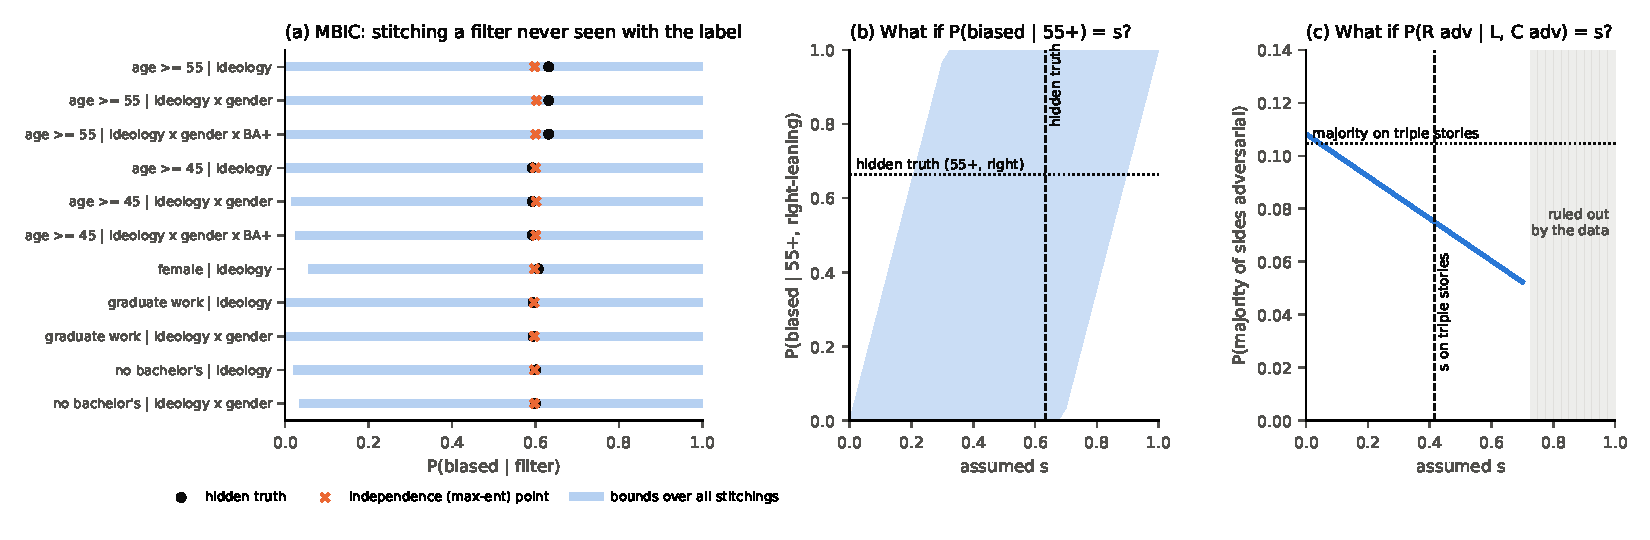
\includegraphics[width=\linewidth]{grey_chart.pdf}
\caption{Grey contexts. (a) MBIC: $P(\text{biased}\mid\text{filter})$ bounded from $\{X,Y\}$ and $\{X,\text{filter}\}$, observed on different halves of the annotators (median over 50 splits), against the hidden truth and the independence (max-ent) point. $X$ is ideology, or ideology with gender and degree. (b) MBIC what-if: if $P(\text{biased}\mid55{+})=s$, the bounds on $P(\text{biased}\mid55{+},\text{right-leaning})$; the data rule out no value of $s$. (c) AllSides what-if: if $P(R\text{ adversarial}\mid L,C\text{ adversarial})=s$, the identified $P(\text{majority adversarial})$; the data rule out $s>0.70$ (grey). Dashed: the value on triple-covered stories.}\label{fig:grey}
\end{figure}

\textbf{MBIC validation} (Figure~\ref{fig:grey}a). The joint of an annotator filter with the bias label is hidden. The engine sees $\{X,Y\}$ from one random half of the annotators and $\{X,\text{filter}\}$ from the other, as if the filter's distribution came from a census. The filters are age $\ge55$, age $\ge45$, female, graduate work, and no bachelor's degree; the covariates are ideology, then ideology with gender and degree. Over 50 splits:
\begin{itemize}
  \item The bounds contain the hidden truth every time (coverage $1.00$ for all 11 filter--covariate settings).
  \item They are nearly vacuous: widths $0.95$--$1.00$. The filters are small groups (9\% of annotators are $55{+}$), and the shared covariates hardly predict either the filter or the label. So the data leave $P(Y\mid A)$ almost free.
  \item The independence point is close to the truth (error $0.009$--$0.037$). But that closeness comes from the assumption: age is in fact nearly unrelated to the label here, and the data cannot show it.
\end{itemize}
The honest reading is that this ``what-if colour'' is supplied almost entirely by the stitching assumption. A report should show the band together with the point.

\textbf{What-if curves.}
\begin{itemize}
  \item \emph{MBIC} (Figure~\ref{fig:grey}b). Every hypothesis $P(\text{biased}\mid55{+})=s$ is consistent with the data. Each still constrains the right-leaning subgroup: at $s=0.875$ that subgroup's rate must be at least $0.60$, and at $s=0.125$ at most $0.40$.
  \item \emph{AllSides} (Figure~\ref{fig:grey}c). The hypothesis on the triple closes the loop (Proposition~\ref{prop:grey}(3)), so each $s$ gives one value of $P(\text{majority adversarial})$, falling linearly from $0.108$ at $s=0$ to $0.052$ at $s=0.70$. Values $s>0.70$ are ruled out (slack $0.002$--$0.012$). The triple-covered stories show $s=0.415$, which is consistent, and there the identified majority is $0.077$. The observed majority on those stories is $0.105$. This is the centre--right population shift of Section~\ref{sec:bounds}, seen again.
\end{itemize}

\subsection{Several conditionals at once: monad, adjunction, and why not cup products}\label{sec:multicond}
A natural next request is a \emph{multi-conditional} what-if: impose several conditions at once and ask which combinations are possible and what they imply. One proposal assigns a categorical tool to each step:
\begin{itemize}
  \item build the space of candidate predictions by the extension adjoint;
  \item prune it by restriction to the observed tables (the counit condition);
  \item mask contradictory combinations of conditions by the cup product of their cocycles, declaring them compatible iff the product class vanishes.
\end{itemize}
The first two steps are what Sections~\ref{sec:bounds}--\ref{sec:grey} already do. The candidate space is the preimage $R^{-1}(e)$, the polytope of global laws. It belongs to the right-adjoint side (preimage) of the Galois connection of Proposition~\ref{prop:kerneladj}; it is not a free extension. Pruning by restriction is the equality constraints. The third step fails (\texttt{examples/multi\_conditional/run.py}, \texttt{tests/test\_multi\_conditional.py}).

\begin{proposition}[Several conditionals]\label{prop:multicond}\st{proved; checked}
\leavevmode
\begin{enumerate}
  \item \emph{Cup products cannot mask.} On every cover in this paper the Čech nerve has $H^2=0$:
  \begin{itemize}
    \item triangle and CHSH cycle: Betti numbers $(1,1)$;
    \item star covers of grey contexts: $(1,0)$.
  \end{itemize}
  So the cup product of any two degree-one classes is zero, and the mask would declare every combination of conditions compatible.
  \item \emph{The right count.} The data leave free exactly the directions of $\ker R$ (signed measures with vanishing restrictions). At most $\dim\ker R$ conditionals can be imposed independently. Their independence is the rank of the hypothesis rows restricted to $\ker R$. Any further condition is either implied by the others or contradicts them.
  \item \emph{The right mask.} A set of conditions is jointly possible iff the linear system (data equalities plus hypothesis rows) is feasible. When it is not, the minimal $L^1$ slack measures how far apart the conditions are. Two conditions can each be possible alone and jointly impossible.
  \item \emph{The monad's part.} Chaining conditionals, e.g.\ $P(Y\mid A)=\sum_xP(Y\mid x)P(x\mid A)$, is the Kleisli composite of the kernels $A\to X\to Y$, i.e.\ the multiplication $\mu$. It is exact only under conditional independence (the maximum-entropy gluing). The bounds are the range over all composites consistent with the data.
\end{enumerate}
\end{proposition}
\begin{proof}
(1) The Betti numbers are computed by \texttt{bounds.nerve\_betti}; no cover here has a non-empty triple overlap of contexts that also bounds a 2-cycle. (2) The feasible set is $(P_0+\ker R)\cap\Delta$. A hypothesis row $\langle a,P\rangle=0$ constrains only its component along $\ker R$, so the number of independent constraints is the rank of the matrix $(a_i^\top K)$, where $K$ is a basis of $\ker R$. (3) Feasibility of a linear system is decided by the LP; the slack programme is Section~\ref{sec:grey}'s. (4) The sum over $x$ is the matrix product of the two stochastic matrices, which is $\mu\circ\mathcal G(g)\circ f$. Replacing $P(Y\mid x,A)$ by $P(Y\mid x)$ is the conditional-independence assumption.
\end{proof}

\begin{figure}[!htbp]\centering
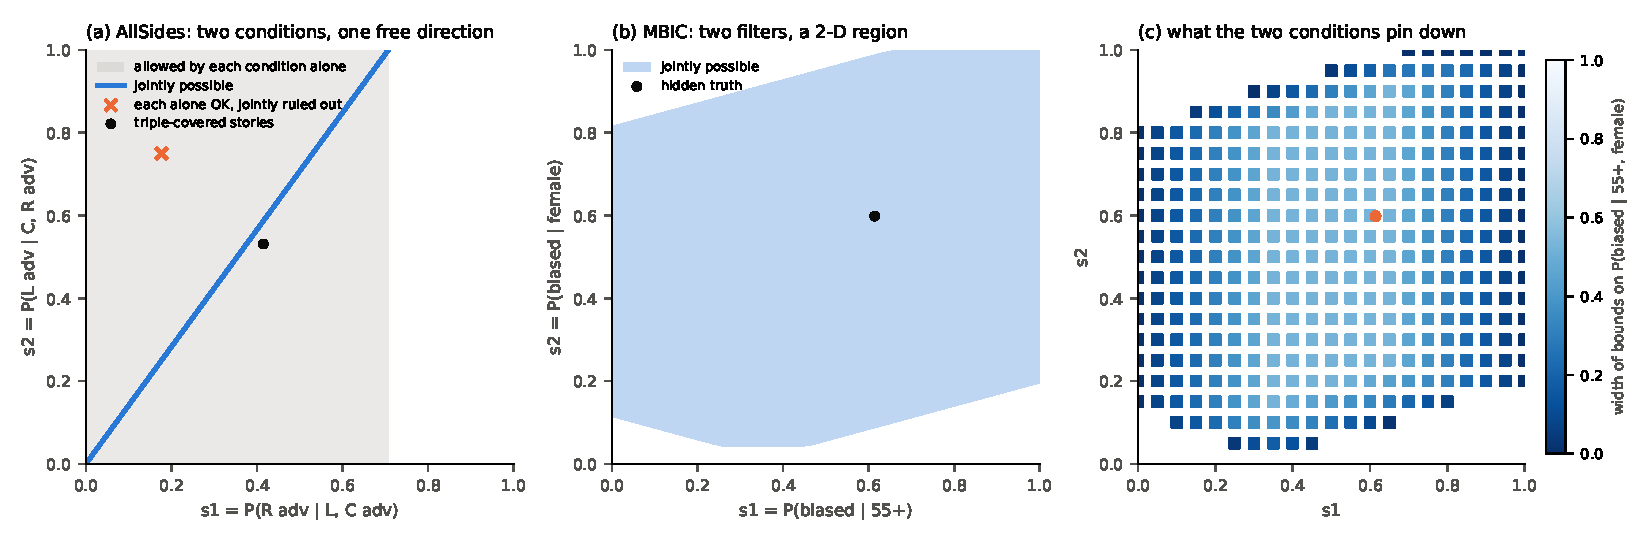
\includegraphics[width=\linewidth]{multi_conditional.pdf}
\caption{Several conditionals. (a) AllSides triangle: two conditions on the never-observed triple. Each alone allows the grey box. Jointly they lie on a line, since $\dim\ker R=1$. The cross is a pair allowed by each condition alone but jointly ruled out. The dot is the triple-covered stories, off the line by the centre--right population shift. (b) MBIC, filters $55{+}$ and female: the jointly possible region of $(P(\text{biased}\mid55{+}),P(\text{biased}\mid\text{female}))$ is two-dimensional. (c) Width of the bounds on $P(\text{biased}\mid55{+},\text{female})$ at each jointly possible pair; dot: the hidden truth.}\label{fig:multicond}
\end{figure}

\textbf{AllSides} (Figure~\ref{fig:multicond}a). We impose two conditions on the never-observed triple, $s_1=P(R\mid L,C)$ and $s_2=P(L\mid C,R)$, both for ``adversarial''.
\begin{itemize}
  \item Each alone is possible on a range ($s_1\in[0,0.707]$, $s_2\in[0,1]$). But $\dim\ker R=1$ and the rank of the two conditions is $1$, so jointly $s_2$ is a \emph{function} of $s_1$ (the $s_2$-range has width $2\times10^{-7}$): $0.177\mapsto0.250$, $0.530\mapsto0.750$.
  \item The pair $(0.177,0.750)$ is allowed by each condition alone but jointly ruled out (slack $0.014$), while the cup-product mask would call it compatible.
  \item The triple-covered stories give $(0.415,0.531)$. The line predicts $0.587$ for $s_2$ at that $s_1$, so these stories are off it: the population shift of Section~\ref{sec:bounds}, detected a third way.
\end{itemize}

\textbf{MBIC} (Figure~\ref{fig:multicond}b,c). Two annotator filters, $55{+}$ and female. The data are $\{I,Y\}$ from one half of the annotators and the population table $\{I,A,F\}$ from the other. Now $\dim\ker R=9$ and the two conditions are independent (rank $2$):
\begin{itemize}
  \item $81\%$ of the $21\times21$ grid of $(s_1,s_2)$ is jointly possible.
  \item Imposing both at their true values narrows the bounds on $P(\text{biased}\mid55{+},\text{female})$ from $[0,1]$ to $[0.412,0.937]$, which contains the hidden truth $0.608$.
  \item It narrows $P(\text{biased}\mid\text{neither})$ from $[0.239,1]$ to $[0.550,0.625]$, which contains $0.576$.
\end{itemize}
The Kleisli composite under conditional independence gives $0.591$ for the first, close to the truth but again by assumption.

\noindent So the multi-conditional algebra the engine needs has three parts:
\begin{itemize}
  \item the preimage polytope (adjunction);
  \item linear feasibility, with slack, as the compatibility mask, and the count $\dim\ker R$ of independent conditions (loop space);
  \item Kleisli composition for chaining conditionals under an explicit independence assumption (monad).
\end{itemize}
Cup products enter only when a cover has a two-dimensional nerve with $H^2\ne0$, for example contexts with genuine triple overlaps in a three-way design. None of our corpora has one.

\subsection{Second-order holonomy: covers whose nerve is a sphere}\label{sec:higher}
Second-order holonomy needs 2-cells. One proposal fits ``intertwiner'' matrices between alternative chains of kernels and reads a trace as a class in $H^2$. That fails on four counts:
\begin{itemize}
  \item comparing two paths with the same ends is first-order, since one path followed by the reverse of the other is a loop;
  \item stochastic matrices are invertible only when they are permutations;
  \item kernels do not form a 2-group;
  \item a trace is not a cohomology class.
\end{itemize}
In fact the 2-cells come with the cover. In the nerve, a set of contexts spans a simplex iff they share a measurement. The \emph{path 2-groupoid} of the nerve then has the contexts as objects, overlaps as 1-cells, and triple overlaps as 2-cells, i.e.\ homotopies between paths of overlaps (\texttt{amb\_vigneaux/higher.py}, \texttt{examples/higher/run.py}, \texttt{tests/test\_higher.py}). A loop of the context graph that bounds 2-cells is filled: any obstruction around it is pushed up to $H^2$.

\begin{proposition}[Covers whose nerve is a sphere]\label{prop:higher}\st{proved; checked}
Let $n$ binary measurements be observed $n-1$ at a time and never all together, i.e.\ the contexts are all $(n-1)$-subsets.
\begin{enumerate}
  \item The nerve is the boundary of the $(n-1)$-simplex, the sphere $S^{n-2}$. Any $k\le n-1$ contexts share $n-k\ge1$ measurements and all $n$ share none. Its Betti numbers are $(1,0,\dots,0,1)$. For $n=4$ (contexts $abc,abd,acd,bcd$) the context graph has $3$ loops, and all $3$ are filled by 2-cells.
  \item $\ker R$ is spanned by the top parity $\chi_n=(-1)^{x_1+\dots+x_n}$. So an outcome $f$ is identified iff $\langle f,\chi_n\rangle=0$, and otherwise its bounds have width along $\chi_n$. For $n=3$ this is the triangle of Proposition~\ref{prop:bounds}(3).
  \item \emph{The obstruction can live entirely at second order.} Take the \emph{higher PR box} on $n=4$: every triple uniform on even parity. Mix it with noise at weight $\lambda$:
  \begin{itemize}
    \item every pair marginal is uniform for every $\lambda$, so the pair cover glues and any pairwise or loop-based (first-order) method sees nothing;
    \item the triple cover has $\CF=\tfrac98(\lambda-\tfrac13)_+$, contextual for every $\lambda>\tfrac13$;
    \item $\gamma\ne0$ only at $\lambda=1$, the same probabilistic-but-not-cohomological gap as for CHSH, one dimension up.
  \end{itemize}
\end{enumerate}
\end{proposition}
\begin{proof}
(1) This is the nerve computation stated, followed by the homology of the boundary of a simplex. The filled loops are computed by checking that each spanning-tree cycle lies in the image of $\partial_2$. (2) The $(n-1)$-marginals fix every log-linear interaction except the top one. A signed measure with all $(n-1)$-marginals zero is therefore a multiple of $\chi_n$ for binary measurements: $\dim\ker R=1$, checked for $n=3,4,5$. (3) Restricting a triple uniform on even parity to a pair gives the uniform law, and noise is uniform. The $\CF$ formula is checked at several $\lambda$ in the tests; the threshold $\tfrac13$ is exact to $10^{-4}$.
\end{proof}

\begin{figure}[!htbp]\centering
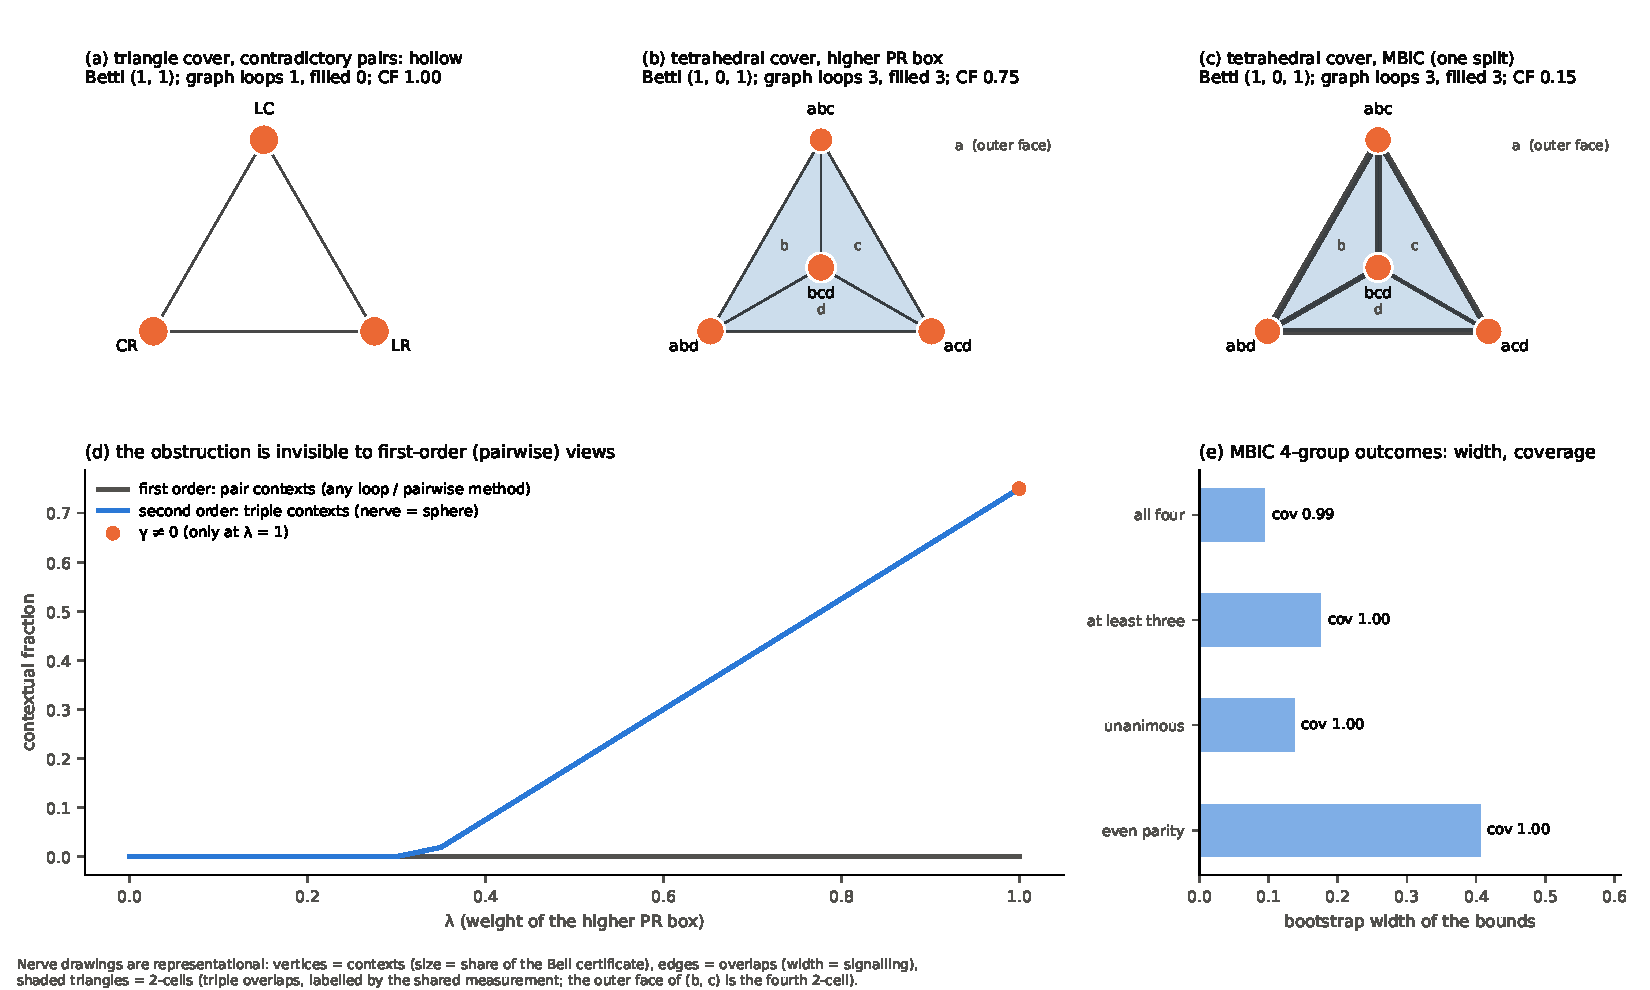
\includegraphics[width=\linewidth]{higher_chart.pdf}
\caption{Second-order holonomy. (a--c) Representational drawings of the nerve (\texttt{higher.plot\_complex}). Vertices are contexts, sized by their share of the Bell certificate. Edges are overlaps, with width proportional to signalling. Shaded triangles are 2-cells, labelled by the shared measurement; in the tetrahedral drawings the outer face is the fourth 2-cell.
(a) Triangle cover with contradictory pairs: hollow, Betti $(1,1)$, the loop is open.
(b) Tetrahedral cover with the higher PR box: Betti $(1,0,1)$, all three graph loops filled, $\CF=0.75$.
(c) The same cover on MBIC four ideology groups, one split; the thick edges are sampling signalling.
(d) Contextual fraction of the higher PR box mixed with noise, in the first-order view (pair contexts) and the second-order view (triple contexts).
(e) MBIC four-group outcomes: bootstrap width of the bounds and coverage of the held-out truth (including its sampling noise).}\label{fig:higher}
\end{figure}

\textbf{MBIC with four ideology groups} (Figure~\ref{fig:higher}c,e). The groups are political-ideology bins $[-10,-5]$, $[-4,0]$, $[1,5]$, $[6,10]$, and each group's outcome is the group majority ``biased''. 1,200 sentences are rated by all four groups. In each of 100 random five-way splits, each triple context comes from its own fifth of the sentences and the four-way truth from the last fifth.
\begin{itemize}
  \item None of the four outcomes is identified: $\langle f,\chi_4\rangle=+1,-3,+2,+8$ for ``all four'', ``at least three'', ``unanimous'' and ``even parity''.
  \item Bootstrap widths are $0.095$, $0.175$, $0.137$ and $0.406$.
  \item Coverage of the held-out truth, including its sampling noise, is $0.99$--$1.00$. The plug-in intervals are much narrower and cover poorly (``all four'': $0.27$), so the bootstrap widening is needed.
  \item The split tables show $\CF$ with median $0.11$ and $\gamma=0$ in every split. Built from the same sentences, the four tables give $\CF=0$. So the $0.11$ is the sampling floor for about $240$ sentences per context, not a four-way obstruction.
\end{itemize}
This is the instrument for a corpus whose sources are observed three at a time and never all together. Such a corpus is the only place a second-order obstruction can hide from every loop-based test.

\subsection{The toric geometry of the sphere covers, component by component}\label{sec:toricsphere}
On a sphere cover the data leave one coordinate free (Proposition~\ref{prop:higher}). It is linear: the fibre is a flat segment, its jets are trivial, and ``second order'' there refers to the topological degree of the nerve, not to jet order. Genuine nonlinear geometry enters through the log-linear (toric) description of the same coordinate. We keep four components separate, so that the effect of each can be read on its own (\texttt{amb\_vigneaux/toric.py}, \texttt{examples/toric/run.py}, \texttt{tests/test\_toric.py}):
\begin{itemize}
  \item[\textbf{[F]}] \emph{Fibre} (mixture coordinate, linear). The consistent global laws form the segment $P_0+t\chi_n$ inside the simplex, with coordinate $m=\langle\chi_n,P\rangle$. The $(n-1)$-way data fix the segment and prefer no point on it. Its image under an outcome is the bounds of Section~\ref{sec:bounds}.
  \item[\textbf{[T]}] \emph{Toric variety} (exponential coordinate). The top log-linear interaction is $\theta=2^{-n}\sum_x\chi_n(x)\log P(x)$. The model without it is $\theta=0$: the single binomial $\prod_{\chi=+1}p=\prod_{\chi=-1}p$, of degree $2^{n-1}$ \cite{gms06}. This is the curved object.
  \item[\textbf{[I]}] \emph{Interaction} (needs the full joint). $\hat\theta$ from units on which all $n$ measurements are observed, with delta-method standard error $2^{-n}(\sum_x1/n_x)^{1/2}$. It also locates the observed law on the segment.
  \item[\textbf{[S]}] \emph{Strata} (support). The faces of the closure of the toric model, and the exact AMB toggle radius of each cell (Proposition~\ref{prop:ambtoggle}, solved by MILP), compared with the saturated radius $-\log(1-p_c)$.
\end{itemize}

\begin{proposition}[Fibre meets variety once]\label{prop:birch}\st{proved; checked}
Along the segment, $\theta$ is strictly increasing from $-\infty$ to $+\infty$, because $d\theta/dt=2^{-n}\sum_x1/P(x)>0$. So the segment meets the toric variety in exactly one point. That point is the maximum-entropy member of the fibre (Birch's theorem \cite{birch63}), which IPF finds. If the segment misses the simplex, the family is contextual: [F] is empty, and so are its intersections with [T] and [S].
\end{proposition}
\begin{proof}
$\theta(P_0+t\chi)=2^{-n}\sum_x\chi(x)\log(P_0(x)+t\chi(x))$, whose derivative is $2^{-n}\sum_x\chi(x)^2/P(x)$. At the ends of the segment some cell with $\chi=\pm1$ vanishes, sending $\theta$ to $\pm\infty$. Maximum entropy on the fibre is attained where the gradient of entropy, $-\log P$, is orthogonal to $\chi$, i.e.\ at $\theta=0$. Checked on 50 random laws each for $n=3,4,5$:
\begin{itemize}
  \item $|\text{Birch}-\text{IPF}|\le5\times10^{-15}$, binomial residual $\le2\times10^{-14}$, monotone in every case;
  \item the higher PR box has a signed law with its 3-margins, but positivity needs $t\in[0.1875,-0.0625]$, which is empty.
\end{itemize}
\end{proof}

\begin{figure}[!htbp]\centering
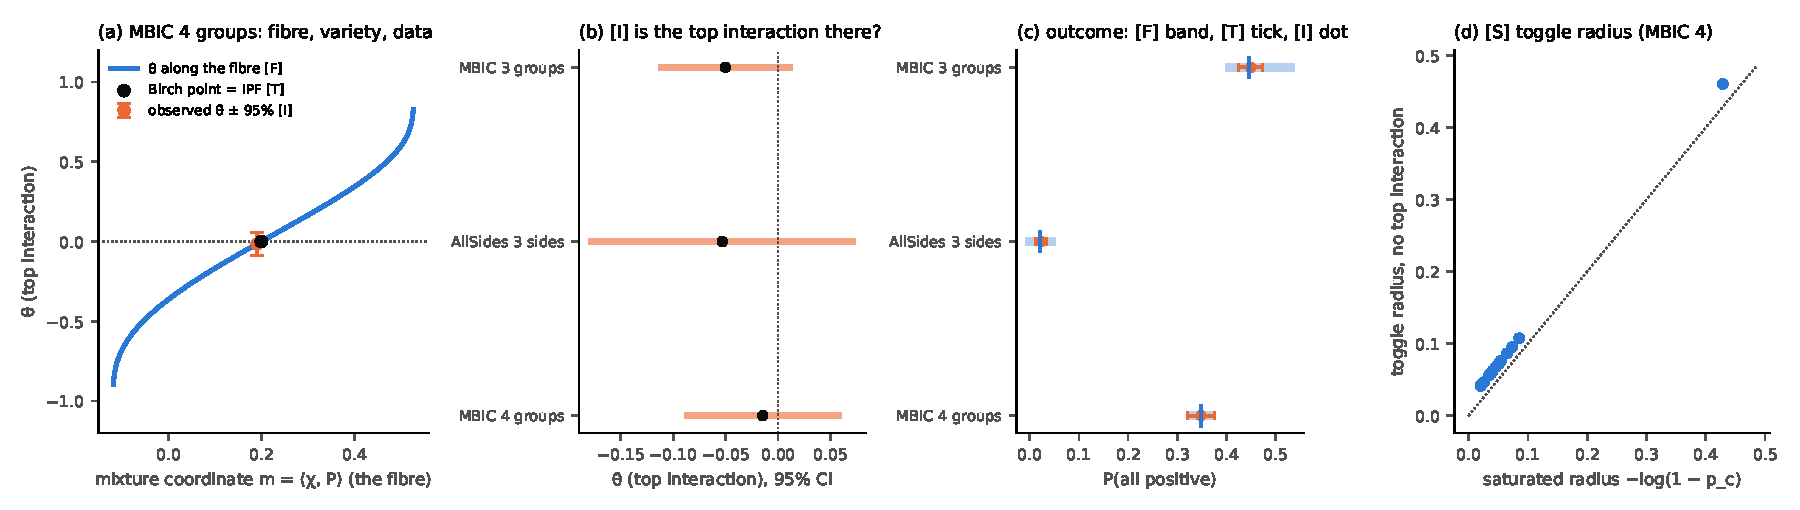
\includegraphics[width=\linewidth]{toric_chart.pdf}
\caption{The four components.
(a) MBIC four groups: $\theta$ along the fibre [F] (mixture coordinate on the horizontal axis); the Birch point, equal to IPF [T]; the observed $\hat\theta$ with its 95\% interval [I].
(b) $\hat\theta$ with 95\% intervals for the three tables with full joints.
(c) One outcome, $P$(all positive), through the components: [F] bounds (band), [F]+[T] maximum-entropy point (tick), [I] observed (dot with interval).
(d) [S] Exact toggle radius of each cell in the no-top-interaction model against the saturated radius (MBIC four groups).}\label{fig:toricsphere}
\end{figure}

\textbf{Real tables with the full joint observed} (Figure~\ref{fig:toricsphere}). The tables are MBIC with three ideology groups (1,600 sentences), AllSides with three sides (736 triple-covered stories) and MBIC with four groups (1,200 sentences).
\begin{center}\small
\resizebox{\linewidth}{!}{\begin{tabular}{lccccc}
\toprule
table & [F] segment in $m$ & [I] $\hat\theta$ (95\% CI) & TV(observed, Birch) & [S] radius / saturated (median, range) & $P$(all): [F] / [F]+[T] / [I]\\
\midrule
MBIC 3 groups & $[-0.923,0.060]$ & $-0.050$ $[-0.111,0.011]$ & $0.016$ & $1.46$ ($1.28$--$3.38$) & $[.407,.530]$ / $.445$ / $.449$\\
AllSides 3 sides & $[0.200,0.557]$ & $-0.053$ $[-0.177,0.071]$ & $0.009$ & $1.53$ ($1.06$--$2.11$) & $[0,.045]$ / $.021$ / $.024$\\
MBIC 4 groups & $[-0.121,0.528]$ & $-0.015$ $[-0.087,0.058]$ & $0.004$ & $1.50$ ($1.07$--$2.05$) & $[.329,.369]$ / $.349$ / $.348$\\
\bottomrule
\end{tabular}}
\end{center}
\begin{itemize}
  \item \emph{[I]: no top-order interaction is detected.} Every interval contains $0$; the closest is MBIC with three groups, $z=-1.61$. Each observed law lies within TV $0.016$ of the Birch point.
  \item \emph{[T] is therefore an accurate gluing here}, and the components separate cleanly on the outcome ``all positive''. [F] alone gives a band of width $0.04$--$0.12$. Adding [T] picks a point in it. [I] confirms the point to within $0.004$, which is the effect of $\theta$ on this outcome.
  \item \emph{[S]: no single cell can be made impossible inside the toric model.} Every minimal forced set has two cells, so the toggle radius exceeds the saturated one by a median factor of about $1.5$ (up to $3.4$). Gluing raises the cost of making an outcome impossible.
\end{itemize}
The pieces are now in place to add curvature as a fifth component: a one-parameter family bent by an external variable (such as poll sponsorship), measured against these four.

\subsection{Curvature: the fifth component}\label{sec:curvature}
The four components above are flat ([F], linear) or flat in natural coordinates ([T], log-linear). Curvature enters when an external variable bends the reported law nonlinearly. We measure it where the data exist: the 2016 presidential polls with sponsor affiliation \cite{econpolls}. These are 2,075 polls from 2016 of likely voters, registered voters or adults, from 252 pollsters; 156 are Democratic-affiliated and 102 Republican-affiliated, each either through the pollster or through the commissioning sponsor (\texttt{amb\_vigneaux/curvature.py}, \texttt{examples/curvature/run.py}, \texttt{tests/test\_curvature.py}).

\textbf{Two geometries of a bend.} Each poll reports a two-party share with natural parameter $\eta_i=\operatorname{logit}p_i$ and Fisher weight $I_i=n_ip_i(1-p_i)$. A sponsorship of intensity $w$ moves the whole vector $\eta(w)$, in one of two ways:
\begin{itemize}
  \item \emph{Shift} ($e$-flat): $\eta_i(w)=\eta_i+w\delta$. This is a straight line in natural coordinates and is exactly how the log-linear component [T] represents any covariate. Its curvature is $0$.
  \item \emph{Pull} ($m$-flat): $p_i(w)=(1-w)p_i+wq$, toward a target $q$. This is straight in probability coordinates and curved in natural ones.
\end{itemize}
The jets are meaningful here: $\eta'(0)$ is the first-order house effect, and $\eta''(0)=-(q-p)^2(1-2p)/(p(1-p))^2$ is its acceleration. Efron's statistical curvature \cite{efron75} at $w=0$,
\[ \gamma^2=\frac{(\eta''^\top I\eta'')(\eta'^\top I\eta')-(\eta'^\top I\eta'')^2}{(\eta'^\top I\eta')^3}, \]
is $0$ for the shift and positive for the pull. Values $\gamma^2\ge\tfrac18$ mean first-order inference about $w$ is unreliable. The two are told apart in data because a shift moves every race by the same logit amount, while a pull moves a race by $w(q-p)/(p(1-p))$, which depends on its baseline.

\textbf{Three sub-components}, each estimated by closed-form weighted least squares or by EM with closed-form steps. The baseline is race (state or national) + two-week period + mode + population, with over-dispersion $\tau^2=0.0027$ estimated from nonpartisan polls. Standard errors are bootstrapped over pollster clusters.
\begin{itemize}
  \item[\textbf{[C1]}] \emph{Velocity} (the first-order bend).
  \begin{itemize}
    \item Democratic-affiliated polls are $\delta_D=-0.050$ logit (SE $0.016$), i.e.\ $2.5$ margin points toward Clinton.
    \item Republican-affiliated polls are $\delta_R=+0.013$ (SE $0.015$, $+0.6$ points), not significant.
    \item The bend is larger when the sponsor commissions the poll ($\delta_D=-0.065$, $\delta_R=+0.028$) than when the pollster itself is affiliated ($-0.039$, $+0.002$).
  \end{itemize}
  \item[\textbf{[C2]}] \emph{Curvature.}
  \begin{itemize}
    \item The slope $\kappa$ of sponsored residuals on the race baseline, which is $0$ under a shift, is $+0.050$ (cluster SE $0.062$) for Democratic and $-0.111$ ($0.083$) for Republican affiliation. Neither differs from $0$.
    \item The pull model, with its extra target parameter, barely improves the weighted fit: $98.1\to97.4$ and $89.3\to86.8$.
    \item The whole-sample curvature of the fitted pull family is $\gamma^2\approx5\times10^{-7}$, far below $\tfrac18$.
  \end{itemize}
  The sponsorship bend is therefore an $e$-flat shift: the log-linear description is adequate, and first-order inference about it is reliable.
  \item[\textbf{[C3]}] \emph{The singular point.} Treating sponsorship among the 1,817 nonpartisan polls as hidden gives the mixture $(1-\pi_D-\pi_R)\,\text{honest}+\pi_D\,\text{bent}_D+\pi_R\,\text{bent}_R$. At $\pi=0$ the tangent space collapses, and the likelihood ratio has a boundary null: in $19\%$ of parametric-bootstrap draws it is exactly $0$, and its 95\% point is $3.47$ instead of the $\chi^2$ value. The observed LR is $1.34$ ($p=0.27$): no hidden sponsorship is detectable.
\end{itemize}

\begin{figure}[!htbp]\centering
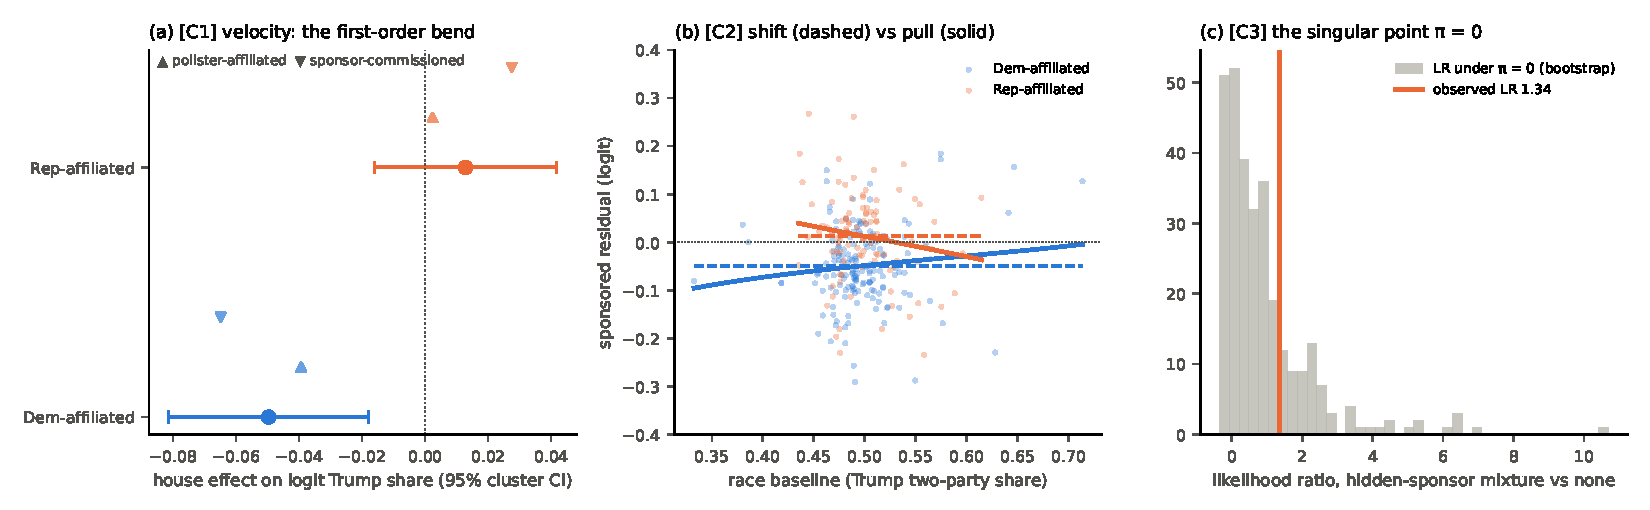
\includegraphics[width=\linewidth]{curvature_chart.pdf}
\caption{Curvature on the 2016 polls.
(a) [C1] House effects of Democratic- and Republican-affiliated polls on the logit Trump share (95\% pollster-cluster intervals), split by pollster-affiliated and sponsor-commissioned.
(b) [C2] Sponsored residuals against the race baseline. Dashed: the shift (constant in logit); solid: the fitted pull. The data do not separate them.
(c) [C3] The likelihood ratio for hidden sponsorship among nonpartisan polls against its parametric-bootstrap null at the singular point $\pi=0$.}\label{fig:curvature}
\end{figure}

\noindent\emph{Where curvature fits.} The five components now answer separate questions:
\begin{itemize}
  \item[\textbf{[F]}] what the lower-order data allow;
  \item[\textbf{[T]}] the log-linear (toric) gluing;
  \item[\textbf{[I]}] whether the top interaction is there;
  \item[\textbf{[S]}] what it costs to make a cell impossible;
  \item[\textbf{[C]}] whether an external modulation is a straight line in the natural coordinates of [T].
\end{itemize}
On these data every answer is the simple one: no top interaction, and a flat, first-order sponsorship bend. The instruments do respond when the structure is present: the tests check that a pull has positive $\gamma^2$ (matching finite-difference jets) while a shift has $\gamma^2=0$, and they recover the weight of a planted hidden mixture.

\subsection{Deformations at the boundary: $T^1$, $T^2$ and the flop}\label{sec:deform}
Deformation theory gives the honest meaning of an ``$\mathrm{Ext}^2$ obstruction''. For a variety $X$ the first-order deformations form $T^1$ and their obstructions lie in $T^2$; for a hypersurface these are $\mathrm{Ext}^1$ and $\mathrm{Ext}^2$ of the cotangent complex. The toric model [T] of a sphere cover is the hypersurface $X=V(f)$, $f=\prod_{\chi=+1}p-\prod_{\chi=-1}p$. It is smooth in the interior of the simplex, so $T^1$ and $T^2$ say something only on the boundary, where the support of the law changes. That is exactly where the AMB (possibilistic) outcome lives (\texttt{amb\_vigneaux/deform.py}, \texttt{examples/deform/run.py}, \texttt{tests/test\_deform.py}).

\begin{proposition}[Deformations of the toric model]\label{prop:deform}\st{proved; checked}
Write $a$ and $b$ for the numbers of even- and odd-parity cells that vanish at a boundary point.
\begin{enumerate}
  \item \emph{Boundary supports.} A set of cells occurs as the zero set of a point in the closure of the model iff it meets both parity classes (checked on all $2^8$ sets for $n=3$ and on all sets of at most four cells for $n=4$). So every support toggle zeros at least one even and one odd cell, which is why every minimal forced set in [S] has two cells.
  \item \emph{Singular locus.} Locally $f\sim x_1\cdots x_a-y_1\cdots y_b$. The model is smooth at the point iff $\min(a,b)=1$, and singular iff $a,b\ge2$; the singular locus inside the local slice has dimension $(a-2)+(b-2)$.
  \item \emph{$T^2=0$.} $X$ is a hypersurface, hence a complete intersection, so every first-order deformation is unobstructed. The ``$\mathrm{Ext}^2$ obstruction'' vanishes identically for these models.
  \item \emph{$T^1$.} The Tjurina number of $x_1\cdots x_a=y_1\cdots y_b$ (computed by a Gr\"obner basis) is:
  \begin{itemize}
    \item $0$ for $\min(a,b)=1$ (smooth);
    \item $1$ for $(2,2)$: the 3-fold node (conifold) $x_1x_2=y_1y_2$, with $T^1$ spanned by the smoothing $x_1x_2-y_1y_2=\varepsilon$;
    \item infinite (non-isolated) for $a+b>4$, but transversally a node at a generic point of the singular locus.
  \end{itemize}
  \item \emph{The flop.} The node has two small resolutions, one for each matching of the two vanishing even cells with the two vanishing odd cells. Statistically, near such a support the model does not determine \emph{which} odd cell is forced together with a given even cell. The AMB toggle (Proposition~\ref{prop:ambtoggle}) picks the cheaper partner, and that choice flips under perturbations as small as the difference of the two partners' masses.
  \item \emph{The top interaction does not smooth.} The level sets $\prod_+p=e^{c}\prod_-p$ of $\theta$ are related by the torus action (rescaling one coordinate), so they are equisingular: the Tjurina number of $x_1x_2=e^cy_1y_2$ is $1$ for every $c$. Changing $\theta$ ([I]) never resolves a node, and the $T^1$ direction (an additive relaxation of the binomial) is not a log-linear deformation.
\end{enumerate}
\end{proposition}
\begin{proof}
(1) $f$ vanishes with some cell zero iff both monomials vanish, i.e.\ the zero set meets both classes. Facial sets are characterised by the LP of Section~\ref{sec:toricstrata}, and the enumeration is in the tests. (2) $\partial f/\partial p_i$ is the monomial with $p_i$ removed, so all partials vanish iff at least two cells of each class vanish. (3) A hypersurface is a local complete intersection, for which $T^2=0$ \cite{hartshorne10}. (4) The Gr\"obner computations are in \texttt{deform.tjurina}. Localising at a point of the singular locus where exactly two cells of each class vanish turns the remaining factors into units and leaves the node. (5) The conifold's two small resolutions blow up the planes $\{x_1=y_1=0\}$ or $\{x_1=y_2=0\}$, i.e.\ the two matchings \cite{atiyah58}. (6) Rescaling $y_1\mapsto e^{c}y_1$ maps one level set to another.
\end{proof}

\begin{figure}[!htbp]\centering
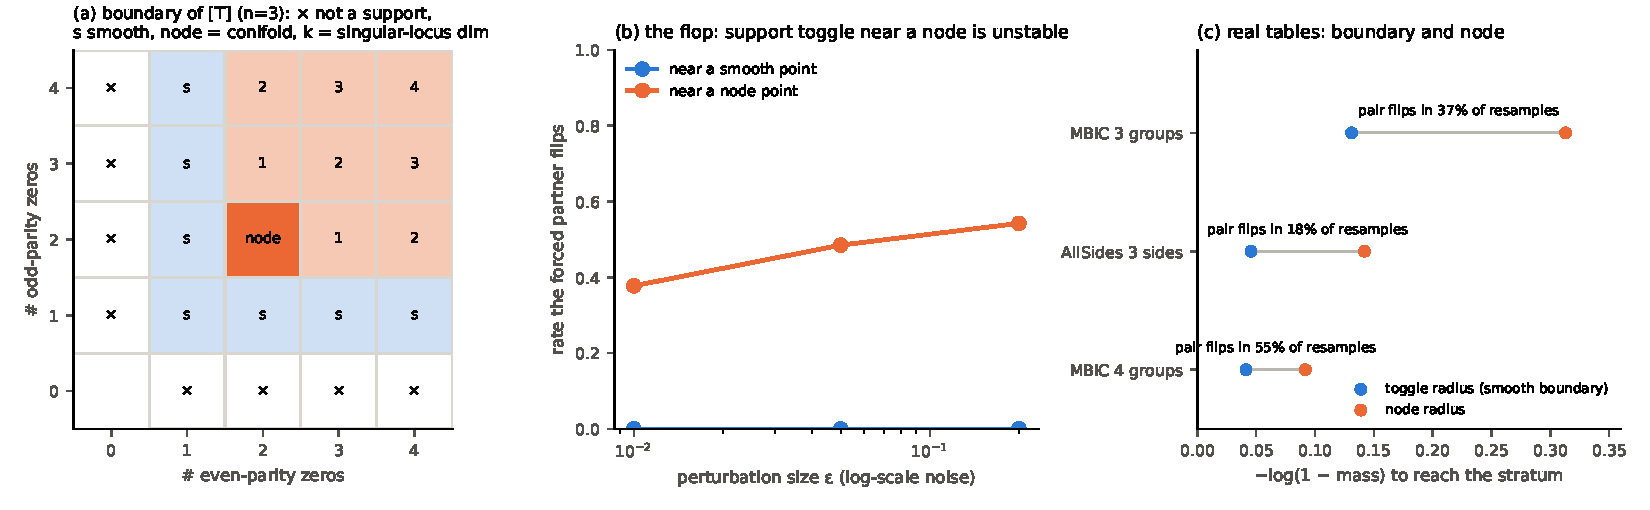
\includegraphics[width=\linewidth]{deform_chart.pdf}
\caption{Deformations at the boundary.
(a) The boundary of the toric model for $n=3$, indexed by the numbers of vanishing even and odd cells: $\times$ does not occur, s is smooth, node is the conifold (Tjurina number $1$), and $k$ is the dimension of the singular locus (transversally a node).
(b) The flop: how often the toggle's forced odd partner changes under multiplicative perturbations, near a smooth boundary point and near a node.
(c) Real tables: the distance to the smooth boundary (toggle radius) and to the nearest node, and how often the toggle's forced pair changes under multinomial resampling of the table.}\label{fig:deform}
\end{figure}

\textbf{The flop, computed} (Figure~\ref{fig:deform}b). Near a smooth boundary point (one even and one odd cell small) the exact MILP toggle returns the cheapest even--odd pair, and its partner never changes under perturbations of $1$--$20\%$. Near a node (two even and two odd cells small, partner margin $0.002$) the partner changes in $38$--$54\%$ of perturbations.

\textbf{Real tables} (Figure~\ref{fig:deform}c).
\begin{center}\small
\begin{tabular}{lcccc}
\toprule
table & toggle radius & node radius & partner margin & forced pair changes under resampling\\
\midrule
MBIC 3 groups & $0.131$ & $0.313$ & $0.16$ & $37\%$\\
AllSides 3 sides & $0.046$ & $0.142$ & $0.43$ & $18\%$\\
MBIC 4 groups & $0.041$ & $0.092$ & $0.11$ & $55\%$\\
\bottomrule
\end{tabular}
\end{center}
\begin{itemize}
  \item All three laws are interior points, where the model is smooth and $T^1=T^2=0$.
  \item The node is only two to three times farther away than the smooth boundary, and the cheapest pairs are close in mass. So \emph{which} pair of outcomes the support toggle would make impossible is not determined by the data: it changes in $18$--$55\%$ of multinomial resamples.
  \item The cost of a toggle (its radius) is stable. Its \emph{identity} is not: a node is close, and the two matchings compete.
\end{itemize}

\noindent So the deformation theory of the model has three contents:
\begin{itemize}
  \item $T^2=0$: no obstructions anywhere;
  \item $T^1$ at the nodes: one smoothing direction, which is not statistical;
  \item the flop at the nodes, which is statistical: an ambiguity in which outcomes become impossible together.
\end{itemize}
A report of a support toggle should therefore give its forced pair together with its resampling stability.

\subsection{Singular statistics and optimal learning: what changes in the outcomes}\label{sec:singular}
Several of our models are singular: the Fisher information degenerates on a set of true parameters. Examples are the hidden-sponsorship mixture at $\pi=0$, latent-class (secant) models, the merge strata of the hierarchy, and the nodes of [T]. There the Bayes free energy is
\[ F_n=nS_n+\lambda\log n-(m-1)\log\log n+O_p(1), \]
where $\lambda\le d/2$ is the real log canonical threshold (learning coefficient) and $m$ its multiplicity. The Bayes generalisation error is $\lambda/n$, and posterior averaging is the optimal learner; plug-in maximum likelihood is not asymptotically normal \cite{watanabe,watanabe18,wbic}. The RLCT is the largest pole $-\lambda$ of the zeta function $\zeta(z)=\int K(w)^z\varphi(w)\,dw$ of the Kullback--Leibler divergence $K$ under the prior $\varphi$, and $m$ is the order of that pole \cite{watanabe}. We measure the \emph{net difference} this makes to each outcome by computing the regular (plug-in) answer and the singular-aware (Bayes) answer on the same data. Everything is done with random-walk Metropolis at inverse temperatures $\beta$, with no gradient steps (\texttt{amb\_vigneaux/singular.py}, \texttt{examples/singular/run.py}, \texttt{tests/test\_singular.py}). The tools are:
\begin{itemize}
  \item WBIC $=\mathrm{E}_{\beta_1}[nL_n]$ at $\beta_1=1/\log n$;
  \item Watanabe's estimate $\hat\lambda=(\mathrm{E}_{\beta_1}-\mathrm{E}_{\beta_2})[nL_n]/(1/\beta_1-1/\beta_2)$, with $\beta_2=1.5/\log n$, averaged over six chains for Monte-Carlo errors;
  \item log marginal likelihoods by thermodynamic integration \cite{gelmanmeng};
  \item a Dirichlet posterior for the flop. Treating the units of a table as exchangeable, de Finetti's theorem (in its categorical form \cite{fgp21}) is what licenses a single latent law with a prior over it.
\end{itemize}

\textbf{Calibration.} We use the shift mixture $(1-a)N(0,1)+aN(b,1)$ with $n=2000$:
\begin{itemize}
  \item at a singular truth ($ab=0$), where $K\sim a^2b^2$ gives $\lambda=\tfrac12$ with $m=2$, the estimate is $\hat\lambda=0.35\pm0.07$ over 10 data sets; the downward bias is the $\log\log n$ term of $m=2$;
  \item at a regular truth ($a=0.3$, $b=1$; $\lambda=d/2=1$) it is $0.95\pm0.09$.
\end{itemize}
So the estimator separates singular from regular, as the tests check.

\begin{figure}[!htbp]\centering
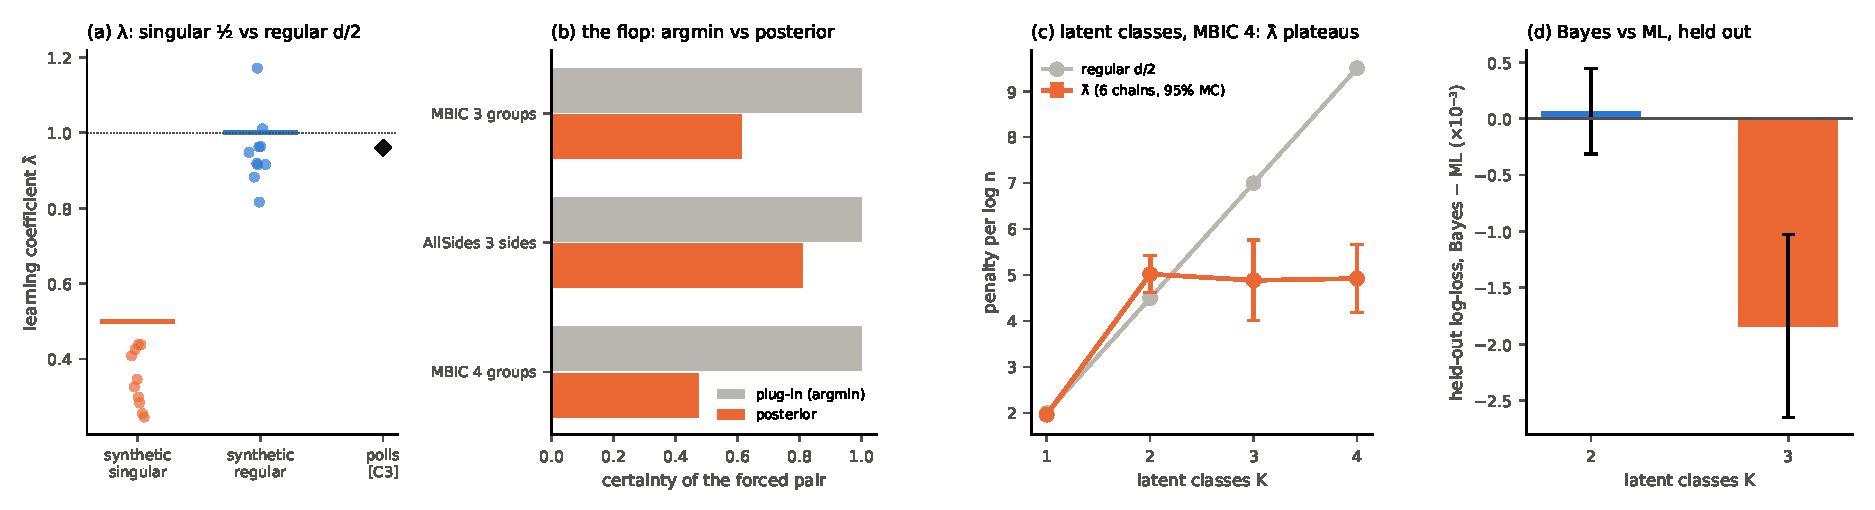
\includegraphics[width=\linewidth]{singular_chart.pdf}
\caption{Singular statistics.
(a) $\hat\lambda$ on synthetic singular and regular truths (bars: theory) and on the polls mixture.
(b) Certainty of the support toggle's forced pair: plug-in argmin (implicitly $1$) against the Dirichlet posterior.
(c) Latent-class models on MBIC four groups: the regular penalty $d/2$ against $\hat\lambda$ (95\% Monte-Carlo intervals). $\hat\lambda$ plateaus near $5$ while $d/2$ keeps growing.
(d) Held-out log-loss per sentence of the Bayes predictive minus ML plug-in (40 random halves; 95\% intervals).}\label{fig:singular}
\end{figure}

\begin{center}\small
\resizebox{\linewidth}{!}{\begin{tabular}{>{\raggedright\arraybackslash}p{0.2\linewidth}>{\raggedright\arraybackslash}p{0.25\linewidth}>{\raggedright\arraybackslash}p{0.3\linewidth}>{\raggedright\arraybackslash}p{0.25\linewidth}}
\toprule
outcome & regular / plug-in & singular-aware / Bayes & net difference\\
\midrule
support toggle: which pair becomes impossible (MBIC 3 / AllSides / MBIC 4) & one pair, implicitly certain & posterior probability $0.61$ / $0.81$ / $0.48$; $3$, $3$, $4$ pairs with $>5\%$ & certainty overstated by $19$--$52$ points\\
support toggle: its radius & $0.131$ / $0.046$ / $0.041$ & $0.128\,[0.113,0.143]$ / $0.045\,[0.031,0.060]$ / $0.039\,[0.030,0.049]$ & negligible: the cost is stable\\
hidden component among 1,817 nonpartisan polls (shift free) & LR $23.2$; regular BIC: present & $\hat\lambda=0.96$; bootstrap of the max-over-$b$ LR (Davies-type null \cite{davies87}, 95\% point $5.35$): $p<0.005$; log Bayes factor (TI) $+4.9$: present; WBIC: a tie within Monte-Carlo error & the component is real but is about $0.3$--$0.8\%$ of polls at $b=-0.275$ logit (about $14$ margin points), $5\times$ the sponsor shift: outlying polls, not hidden sponsorship\\
number of latent classes (MBIC 4 groups) & BIC: $K=2$ decisively (gaps $14$ and $31$ to $K=3,4$) & $\hat\lambda=1.96,\ 5.0,\ 4.9,\ 4.9$ for $K=1..4$ (against $d/2=2,\ 4.5,\ 7,\ 9.5$); WBIC ties $K=2,3,4$ within Monte-Carlo error & BIC over-penalises extra classes by about $2$--$4.6\log n$; $P$(all four) is $0.347$--$0.350$ either way (observed $0.350$)\\
held-out prediction (log-loss per sentence) & ML plug-in & Bayes predictive (posterior average) & $K=2$: $+0.0001\pm0.0002$ (no difference); $K=3$: $-0.0018\pm0.0004$, Bayes better in $72\%$ of splits\\
\bottomrule
\end{tabular}}
\end{center}

\begin{itemize}
  \item \emph{Where singularity changes the outcome.} It changes the \emph{identity} of a support toggle: the plug-in pair is the posterior favourite only $48$--$81\%$ of the time. It changes the \emph{model choice}: extra latent classes cost about $\lambda\approx5$ in total, not $d/2$ each, so BIC's decisive $K=2$ becomes a tie. And it changes \emph{held-out prediction} in the over-parameterised model, where posterior averaging beats the plug-in, as the theory predicts.
  \item \emph{Where it does not.} Toggle costs, the predicted $P$(all four), and the regular-like $K=2$ predictions are unchanged.
  \item \emph{An instructive disagreement.} On the polls, WBIC ties while the Bayes factor and the bootstrap favour a component. WBIC's $\log n$ asymptotics are worst when the signal sits next to the singular set (a tiny weight $a$ with a large shift $b$). The posterior on that ridge also mixes poorly: the posterior mean of $ab$ changes sign between runs. In this regime thermodynamic integration, not WBIC, is the reliable criterion.
\end{itemize}

\section{Probing inside arity: hull trees and the $p$-adic radius profile}\label{sec:hull}
The arity grading records how many sources cover a unit, but not how those sources relate on it. Proposition~\ref{prop:filled} explains why holonomy cannot help. Inside a filled cell every loop of differences on the same unit sums to zero. What survives is the \emph{configuration} of the $k$ values modulo translation, a point of $\R^k/\R\mathbf 1$, and its combinatorial shadow is a tree.

\begin{proposition}[Hull invariants of a filled cell]\label{prop:hull}\st{proved; checked}
Let a unit be covered by $k$ sources with values $x_1,\dots,x_k$.
\begin{enumerate}
  \item Every loop sum $\sum(x_{i_r}-x_{i_{r+1}})$ over sources on the unit is $0$. The class $[x]\in\R^k/\R\mathbf1$ is not constrained.
  \item The \emph{hull tree} (single-linkage dendrogram of $|x_i-x_j|$) and its first merge, the \emph{coalition}, are invariant under the unit effect $x\mapsto x+v_e\mathbf1$. After subtracting source effects they are invariant under every natural change $u_s+v_e$. Coalition frequencies in excess of an additive null are therefore structure inside arity that neither lean nor holonomy detects.
  \item For integer values in $\Z_p$ the hull tree is the convex hull of the $k$ points in the Berkovich line. Its vertices are the discs where the points split. The number of discs of radius $p^{-m}$ containing them is a step function of $m$ with integer jumps, and the class sizes give a composition of $k$ that is refined as $m$ grows.
  \item For sum claims $x_i+x_j=r_{ij}$ over $\Z_p$, let $e(m)=\log_p$ of the order of the obstruction class of $r$ in $\mathrm{coker}(A)\otimes\Z/p^m$. This is canonical: it does not depend on the Smith basis. Then $e(m)=\max_i(\min(m,v_p(d_i))-v_p(c_i))^+$ is piecewise linear with integer slopes in $\{0,1\}$ and finitely many breakpoints. It vanishes exactly for $m\le m^*$ (the local hulls glue at radius $p^{-m^*}$, Proposition~\ref{prop:padicradius}), and it flattens at the torsion ceilings $v_p(d_i)$.
\end{enumerate}
\end{proposition}
\begin{proof}
(1) telescopes. (2) Translation preserves every $|x_i-x_j|$; subtracting $\hat u_s$ removes source effects. (3) Two integers lie in a common disc of radius $p^{-m}$ iff they agree mod $p^m$, and these classes refine as $m$ grows. (4) In Smith form $\mathrm{coker}(A)\otimes\Z/p^m\cong\bigoplus_i\Z/p^{\min(m,v_p(d_i))}$. The $i$-th coordinate $c_i$ of $r$ has order $p^{(\min(m,v_p(d_i))-v_p(c_i))^+}$, and the order of the class is the maximum.
\end{proof}
\noindent Item (4) is the elementary, arithmetic counterpart of the continuity theorems for radius functions on Berkovich curves: continuous, piecewise log-linear with integer slopes, and controlled by a finite graph \cite{pulita}. Only this elementary part transfers. The deformation theory there (canonical $\Sigma$-module structures, quasi-unipotent monodromy) needs a $p$-adic differential equation, which our data do not have. We also use the $p$-adic metric only where the data are arithmetic (counts and sum claims). On real-valued bias scores the $2$-adic distance is semantically arbitrary, so the real dendrogram is used instead.

\textbf{Results} (\texttt{amb\_vigneaux/hull.py}, \texttt{examples/arity\_probe/run.py}).
\begin{itemize}
  \item \emph{MBIC, annotators inside a sentence.} We use the 1{,}640 sentences labelled by left, centre and right annotators (ideology $\le-4$, middle, $\ge3$), with the value being each group's bias rate. The null permutes the group labels within each sentence, which keeps ties, group sizes and rater heterogeneity (ties: $225$ observed, $228$ expected).
    \begin{itemize}
      \item Left and centre annotators agree first far more often than chance: $578$ against $461$ expected, $p<0.002$. The right group is the odd one out: left--right $441$ against $484$ ($p=0.008$), centre--right $396$ against $467$ ($p<0.002$).
      \item The isolation depends on the outlet. On sentences from left outlets the right annotators split from the \emph{left} (left--right $157$ against $194$, $p<0.002$; centre--right $180$ against $194$, $p=0.20$). On sentences from right outlets they split from the \emph{centre} (centre--right $150$ against $187$, $p<0.002$; left--right $191$ against $197$, $p=0.59$).
      \item The ideology leans are about $\pm0.01$, so none of this is lean. It is structure inside a 3-ary cell, invisible to holonomy by Proposition~\ref{prop:filled}. It refines the hostile-media loop of Section~\ref{sec:bias3}.
    \end{itemize}
  \item \emph{AllSides, sides inside a story.} In the 736 story groups covered by left, centre and right, using the tone of Trump sentences, coalition counts equal the additive null ($258/251$, $236/240$, $242/246$). They do not shift at the 2016 election or at COVID ($p\ge0.20$). Tone carries no structure inside arity here.
  \item \emph{NewsWCL50.} Only 6 event $\times$ target cells have at least 3 codes from all five outlets, which is too few to test.
  \item \emph{BASIL.} Stance is coded as a relative ranking within each triplet, for example $(1,0,-1)$, so equal spacing is built in: 68 of 100 triplets are ties against about 30 under the additive null. The probe needs a continuous value for each source.
  \item \emph{Arity grading, $p$-adically} (synthetic; \texttt{examples/arity\_probe/padic\_arity.py}). Units of arity $k$ measure integer source values with errors divisible by $p^{a_k}$ ($a_2=1$, $a_3=2$, $a_4=4$), and each unit contributes sum claims for the pairs it covers.
    \begin{itemize}
      \item The claims of any \emph{single} unit glue at full precision (24 of 24 units): a filled cell is flat, the $p$-adic form of Proposition~\ref{prop:filled}.
      \item Keeping the units of arity $\ge K$, the claims glue to radius $3^{-1}$, $3^{-2}$ and $3^{-4}$ for $K=2,3,4$. The order profiles are $e=(0,0,1,2,\dots)$, $(0,0,0,1,\dots)$ and $(0,0,0,0,0,1,\dots)$.
      \item The arity filtration therefore gives \emph{nested gluing radii}, each set by the precision of its grade, with integer slopes above each radius.
      \item Real bias scores are not arithmetic, so this check is synthetic. On data the real dendrogram of Proposition~\ref{prop:hull}(2) plays this role.
    \end{itemize}
  \item \emph{$p$-adic profile} ($p=3$, two independent even loops on $K_{2,3}$). Errors of $3^4$ on one edge give $e=(0,0,0,0,0,1,2)$, so $m^*=4$. Adding an error of $3^2$ on the other loop gives $e=(0,0,0,1,2,3,4)$, so $m^*=2$. An error of $18=2\cdot3^2$ gives the same profile as $9$, because only the valuation matters. The breakpoint is the gluing radius and the slope is an integer.
\end{itemize}

\subsection{Replication, the lean-invariant variogram, and the bridge to toggling}\label{sec:hull-rep}
Coalition counts depend on the leans. The quantity that does not is the \emph{variogram} of the sources on shared units,
\[
\gamma_{ij}=\tfrac12\operatorname{Var}_{\text{units}}(x_i-x_j),\qquad \gamma^*_{ij}=\gamma_{ij}-\tfrac12\,\mathbb E[v_i+v_j],
\]
where $v_s$ is the sampling variance of source $s$'s value on a unit (for a mean of $n\ge2$ binary raters, $\hat p(1-\hat p)/(n-1)$). The correction stops groups with few raters from being pushed apart by noise alone.

\begin{proposition}[Variogram tree]\label{prop:variogram}\st{proved; checked}
$\gamma_{ij}$ is invariant under every natural change $x_{s,e}\mapsto x_{s,e}+u_s+v_e$. Its single-linkage tree is a tree-level invariant of the family of filled cells. The first merge of that tree, $\arg\min\gamma^*$, is the population coalition.
\end{proposition}
\begin{proof}
$(x_i+u_i+v_e)-(x_j+u_j+v_e)=x_i-x_j+(u_i-u_j)$, and a constant shift does not change a variance.
\end{proof}
\noindent A proposed alternative, ``the coalition tree is non-trivial iff the values are not all equal, its shape is given by the $p$-adic order, and it is invariant under natural recalibrations'', needs three corrections:
\begin{itemize}
  \item the first clause is true but empty;
  \item the $p$-adic order applies only to arithmetic data;
  \item the tree of the raw values is \emph{not} invariant under source recalibration $u_s$. Only the variogram tree, or the tree after removing source effects, is.
\end{itemize}

\begin{proposition}[Majority reads the tree]\label{prop:majority}\st{proved; checked}
For three binary sources with marginals $p_i$ and $\gamma_{ij}=\tfrac12 P(x_i\ne x_j)$,
\[
P(\text{majority}=1)=p_1+p_2+p_3-(\gamma_{12}+\gamma_{13}+\gamma_{23})-2P(x_1=x_2=x_3=1).
\]
With fixed marginals, and hence the same bias cochain, lean and loops, the majority outcome can lie on either side of $\tfrac12$. For example, with all $p_i=0.45$:
\begin{itemize}
  \item independent votes give $0.425$;
  \item all three always agreeing gives $0.45$;
  \item exactly two agreeing on ``biased'' (probability $0.675$, each pair equally often, otherwise all ``unbiased'') gives $0.675$.
\end{itemize}
\end{proposition}
\begin{proof}
$\mathbf 1[\text{maj}]=x_1x_2+x_1x_3+x_2x_3-2x_1x_2x_3$, and $E[x_ix_j]=\tfrac12(p_i+p_j)-\gamma_{ij}$. The examples are checked in \texttt{tests/test\_hull.py}.
\end{proof}
\noindent This is the bridge to Proposition~\ref{prop:toggle}. That proposition covers outcomes that are linear in the mean cochain $b$. A majority outcome, or any AMB outcome that reads the joint support, also reads the variogram tree. A phase change that leaves every mean unchanged, with no natural part and no loop part, can therefore still toggle it. Such a change sits at second order, at the level of the coalition tree, and holonomy cannot see it.

\textbf{Replication} (\texttt{examples/arity\_probe/replicate.py}).
\begin{itemize}
  \item \emph{MBIC, noise-corrected variogram, 3 groups.}
    \begin{itemize}
      \item $\gamma^*_{LC}=-0.002\pm0.003$, $\gamma^*_{LR}=0.005\pm0.003$, $\gamma^*_{CR}=0.014\pm0.004$. The first merge is left--centre (bootstrap support $0.97$). The only clearly non-zero disagreement is centre--right, at 3.3 se.
      \item By outlet type: centre--right is largest on right-outlet sentences ($0.021\pm0.007$) and weaker on left-outlet sentences ($0.008\pm0.006$).
      \item The coalition counts are the same for articles up to 2019 and from 2020, though the ratings were all collected in 2020.
    \end{itemize}
  \item \emph{MBIC, 5 finer groups} ($\le-7$, $-6..-2$, $-1..1$, $2..6$, $\ge7$). No structure: every $|\gamma^*|\le0.011$ with se $0.004$--$0.007$, and the first merge has bootstrap support $0.37$. With fewer raters per group the noise correction dominates. The 3-group result is therefore not refuted, but it does not refine into a finer ideology gradient.
  \item \emph{BABE expert annotators.} Eight annotators rate all 1{,}700 sentences (SG1), or about five per sentence over 3{,}674 sentences (SG2). At the annotator level the variogram does not follow ideology: the Mantel correlation of $\gamma_{ij}$ with $|\text{ideology}_i-\text{ideology}_j|$ is $-0.26$ ($p=0.95$) and $-0.02$ ($p=0.50$). Annotator 1 (right, $+5$) is closest to annotator 10 (left, $-15$). Group-level comparisons in BABE are confounded by individuals: SG1 has one right annotator, and in SG2 groups of at least two raters rarely overlap.
\end{itemize}
\noindent\emph{Assessment.} The coalition structure inside MBIC's 3-ary cells is real and stable over article years: the right crowd is the odd one out, mainly against the centre and mainly on right-outlet sentences. It does not refine to finer ideology groups, and trained experts show no ideology-driven agreement geometry. It is a crowd-annotation effect, not yet a general law.

\section{Moduli: toric strata, tree space, and the singular strata of grammars}\label{sec:moduli}
Moduli language earns its place only where the quotient is not a vector space. The bias tables modulo natural changes form $C^1/\mathrm{im}\,\delta=H^1\cong\R^{\beta_1}$, with the loop sums as coordinates. So do the $\R$-valued character varieties $\mathrm{Hom}(\pi_1,\R)$. Calling these moduli spaces is correct, but it adds no theorem. Three places do add content: the \emph{boundary} of the toric model (AMB outcomes), the \emph{space of trees} (hull and coalition trees), and the \emph{singular strata} of grammar space (hierarchy recovery). Derived and stacky structure is not needed for any result below. It becomes relevant only for long chains of hierarchy levels, and it is deferred.

\subsection{AMB outcomes are boundary strata of the toric model}\label{sec:toricstrata}
A hierarchical log-linear model with design matrix $A$ (the columns $a_j$ record which margins cell $j$ contributes to) is a toric variety. Its closure is a disjoint union of strata, one for each \emph{facial set} $S$: a set of cells that is the zero set of a supporting hyperplane of $\mathrm{cone}(A)$, i.e.\ $h\cdot a_j=0$ on $S$ and $h\cdot a_j>0$ off $S$. The stratum of $S$ is the model restricted to the cells in $S$ \cite{gms06,fr12,efrs06,sullivant}. Under the moment map, strata correspond to faces of the marginal polytope \cite{fulton,cls}. The support of a point, meaning which cells are possible, is its possibilistic (AMB) outcome \cite{ab11}, and Section~\ref{sec:strata} already stratifies the engine by support. What the toric model adds is which supports are \emph{reachable} as limits of the model, and how far away they are. So the outcome layer says \emph{which stratum} a point is in, and the probability layer says \emph{where} it is inside the stratum.

\begin{proposition}[AMB toggle radius]\label{prop:ambtoggle}\st{proved; checked}
Let $p$ lie in the interior of a toric model and let $S$ be a facial set.
\begin{enumerate}
  \item The reverse-KL closest point of the $S$-stratum is $p|_S/p(S)$, at distance $-\log p(S)$. Consequently the smallest change of the probability layer, within the model, that makes cell $c$ impossible is
  \[
  r(c)=\min\{-\log(1-p(F)) : c\in F,\ F^{\rm c}\text{ facial}\}.
  \]
  \item Every Markov move $m=m^+-m^-$ gives $\sum_{j\in m^+}a_j=\sum_{j\in m^-}a_j$. Hence a co-facial set $F$ that meets one side of a move meets the other side. In particular, in the no-three-way (glued) model with $I,J\ge2$, a single cell is never co-facial: \emph{a possibilistic outcome cannot toggle in one context alone}.
\end{enumerate}
\end{proposition}
\begin{proof}
(1) $p|_S/p(S)$ lies in the closure, since facial restrictions of the model are in its closure \cite{gms06}. For any $q$ supported on $S$, $\mathrm{KL}(q\|p)=\mathrm{KL}(q\|p|_S/p(S))-\log p(S)\ge-\log p(S)$ by Gibbs' inequality. (2) Apply $h\ge0$ to the move identity. If $h\cdot a_c>0$ for some $c\in m^+$, then some $j\in m^-$ has $h\cdot a_j>0$. The basic move of any $2\times2\times2$ sub-box then shows that a single-cell $F$ is impossible.
\end{proof}
\noindent We compute $r(c)$ exactly by a mixed-integer program: minimise $\sum_jp_jz_j$ subject to $h\cdot a_j\ge0$, $h\cdot a_j\le Mz_j$, $h\cdot a_c\ge1$. An LP relaxation gives an achievable upper bound. The exact values were checked against brute-force enumeration of all facial sets on $2\times3\times2$. The minimal co-facial sets there include the context, the slice, and loop-shaped sets such as $\{(0,0,0),(1,1,1)\}$ on $2\times2\times2$ (\texttt{amb\_vigneaux/strata.py}).

\textbf{Results} (\texttt{examples/strata/amb\_toggle.py}; evidence in sentences or articles, $N\cdot p(F)$).
\begin{itemize}
  \item \emph{MBIC} (outlet $\times$ topic $\times$ majority label; 176 live cells, with empty outlet--topic contexts as structural zeros). Under the glued model, making a label impossible in one context costs a median of $2.0\times$ the evidence of the saturated model, and up to $17\times$.
    \begin{itemize}
      \item The cheapest toggle removes the \emph{whole context} for 163 cells, a source--label slice for 9, and a topic--label slice for 4. The possibilistic outcome of a single outlet--topic context can only change by losing that context or a whole slice.
      \item The nearest toggles are thin contexts with 3--5 sentences, such as HuffPost$\times$environment and Reuters$\times$student debt.
    \end{itemize}
  \item \emph{AllSides} (side $\times$ topic group $\times$ adversarial, 2015--2020; 48 cells). The median ratio is $1.6\times$. The cheapest toggle is a whole context for 25 cells, a topic slice for 20, and a source slice for 3. For example, ``adversarial is impossible on healthcare'' can only happen for all three sides at once (7 articles).
    \begin{itemize}
      \item Around COVID, the centre's ``adversarial is possible'' outcome moves \emph{closer} to a toggle on justice ($3.7\%\to1.8\%$ of the window's articles), and \emph{further} from one on media ($1.1\%\to3.7\%$) and politics ($2.5\%\to4.7\%$). These are two opposite moves of the same outcome layer, invisible to the pooled alignment of Section~\ref{sec:certificate}.
    \end{itemize}
\end{itemize}

\subsection{Tree space: the coalition test in BHV space}\label{sec:bhv}
Hull, variogram and hierarchy trees are points of the space of phylogenetic trees \cite{bhv}. That space is the tropical moduli space $\overline M_{0,n}^{\rm trop}$ and the Berkovich skeleton of $\overline M_{0,n}$ \cite{speyer,acp}. The $p$-adic and real hull trees of Section~\ref{sec:hull} are therefore the same object read in two settings, and the real points of $\overline M_{0,n}$ are tiled by associahedra \cite{devadoss}, which links trees to the $A_\infty$ structure of Section~\ref{sec:massey}.

For three sources the space $T_3$ is a spider: three half-lines, one per coalition, glued at the star tree. A cell gives the point (coalition, internal edge $h_2-h_1$). The metric is $|s-t|$ on the same leg and $s+t$ across legs. The Fr\'echet mean is \emph{sticky} \cite{hotz}: with leg moments $m_a=E[s\,\mathbf1_a]$, it lies on leg $a$ at $m_a-\sum_{b\ne a}m_b$ when that is positive, and at the origin otherwise. Changes are tested by the energy distance \cite{szekely} with a permutation null (\texttt{amb\_vigneaux/treespace.py}, \texttt{examples/strata/treespace\_run.py}).
\begin{itemize}
  \item \emph{MBIC} (1{,}640 sentences). The mean sticks at the star. The left--centre leg carries excess mass (moment $0.118$ against $0.082$ under within-sentence label permutation, $p<0.002$), and the centre--right leg carries a deficit ($0.067$ against $0.080$). So there is a strong left--centre \emph{tendency}, but not a population coalition: its mass is less than the other two legs together. Left against right outlets: energy $p=0.066$. Articles up to 2019 against 2020: $p=0.23$.
  \item \emph{AllSides} (736 stories, tone). The mean sticks at the star. Before/after the 2016 election $p=0.17$; before/after COVID $p=0.058$, with the left--centre moment rising from $0.058$ to $0.095$ on 85 post-COVID stories. This is suggestive, not significant.
\end{itemize}
In tree space, then, the coalition structure of Section~\ref{sec:hull} is a displacement of mass toward one leg. It never unsticks the mean, and no event moves it significantly at $0.05$.

\subsection{The singular strata of grammar space}\label{sec:gram-strata}
The parameters of a hierarchical grammar, modulo relabelling of the symbols at each level, form a space that is singular along the strata where two symbols at one level coincide. Singular learning theory \cite{watanabe,wbic} says that such strata, not the parameter count, govern what data can resolve. We measured the likelihood distance from the true grammar to each merge stratum. For each level $l$ and each pair of level-$l$ symbols, we average the pair's rows (weighted by usage), collapse the child axes above, and compute the held-out difference in $\log p$, with a paired se over 4{,}000 sequences (\texttt{benchmarks/o6/merge\_strata.py}).

\begin{proposition}[The root level is not identifiable]\label{prop:root}\st{proved; checked}
The likelihood depends on the root level only through the mixture $\sum_s\pi_sP_L[s]$. Merging any two root symbols with usage weights leaves $\log p(x)$ exactly unchanged. Root-symbol structure lies on a positive-dimensional fibre of constant likelihood, and no learner can recover it from data.
\end{proposition}
\begin{proof}
$p(x)=\sum_s\pi_s\sum_{a,b}P_L[s,a,b]\,\beta_a\beta_b$, where $\beta$ are the inside values of the children. Replacing $s,s'$ by one symbol with prior $\pi_s+\pi_{s'}$ and rule row $(\pi_sP_L[s]+\pi_{s'}P_L[s'])/(\pi_s+\pi_{s'})$ leaves the sum unchanged. (Checked exactly in \texttt{tests/test\_root\_identifiability.py}.)
\end{proof}
\begin{center}\small
\begin{tabular}{lcccccc}
\toprule
$\Delta$: median (min) & level 1 & 2 & 3 & 4 & 5 & 6\\
\midrule
$V=8$, $L=6$ & $5.07$ ($1.37$) & $2.28$ ($0.93$) & $0.99$ ($0.43$) & $0.37$ ($0.07$) & $0.13$ ($0.035$) & $\mathbf 0$ (all)\\
$V=16$, $L=4$ & $0.69$ ($0.17$) & $0.27$ ($0.13$) & $0.14$ ($0.0016$) & $\mathbf 0$ (all) & & \\
\bottomrule
\end{tabular}
\end{center}
\begin{itemize}
  \item Every pair of used symbols below the root is resolvable ($\Delta>2$ se). The merge distance falls by about $2.5$--$3\times$ per level toward the top, and it is exactly $0$ at the root.
  \item This resolves the O6 finding that ``likelihood does not certify structure''. The worst top-level shortfalls of the baseline, $0.55$ against $0.88$ at level 4 of $V=16$, $L=4$ and $0.39$ against $0.74$ at level 6 of $L=6$, are at the \emph{root}. Root recovery is not a well-posed target, and the ``Bayes ceiling'' there uses the true grammar and is unattainable. The O6 scorer now marks the root level as non-identifiable, and structure is scored on levels $1\dots L-1$.
  \item At $L=6$ the likelihood gap EM leaves ($0.005$) is below every level-5 merge distance ($\ge0.035$). The level-5 shortfall is therefore slow EM along weakly curved directions, not a likelihood blind spot. At $V=16$, $L=4$ one level-3 pair costs only $0.0016$ nats, below the $0.02$ gap: there the likelihood genuinely cannot separate that pair at this sample size.
  \item Split--merge (Section~\ref{sec:o6}) moves the model onto a merge stratum and leaves it along another branch. It crosses between basins through the singular locus, a move that EM's small uphill steps do not make.
  \item Below the root, generic identifiability of latent tree models up to relabelling \cite{amr09} agrees with the positive merge distances measured here.
\end{itemize}

\subsection{Split--merge and the learning coefficient}\label{sec:splitmerge-rlct}
Singular learning theory makes the merge-strata picture quantitative \cite{watanabe,watanabe18}. The RLCT $\lambda$ is the largest pole $-\lambda$ of $\zeta(z)=\int K(w)^z\varphi(w)\,dw$, where $K$ is the Kullback--Leibler divergence to the truth and $\varphi$ the prior. The Bayes free energy is $F_n=nS_n+\lambda\log n-(m-1)\log\log n+O_p(1)$, and the Bayes generalisation error is $\lambda/n$. A merge stratum is part of the singular set of the split model. We test what this implies for split--merge on a single grammar node: a parent symbol emits $d$ children independently, each categorical on $V$ symbols, i.e.\ a latent-class model (\texttt{singular.cat\_lca\_*}, \texttt{examples/splitmerge/run.py}). $\hat\lambda$ is Watanabe's two-temperature estimate over four Metropolis chains (Section~\ref{sec:singular}).

\begin{proposition}[Learning coefficients at merge strata]\label{prop:splitrlct}\st{(1) proved; (2)--(3) computed}
\leavevmode
\begin{enumerate}
  \item \emph{A lone node contributes nothing.} If a node's children are a single categorical draw on $V^2$ cells, every $K$ gives the same family (a mixture of categoricals is a categorical). Extra symbols therefore leave $K(w)$ unchanged along whole fibres, and $\lambda$ is that of the saturated categorical, $(V^2-1)/2$, for every $K$. This is Proposition~\ref{prop:root} in learning-coefficient form: the root's symbol structure adds $0$ to $\lambda$, and no amount of data resolves it. On $V^2=16$, $n=3000$: $\hat\lambda=7.37,\ 7.20,\ 8.28,\ 7.72$ for $K=1..4$ (theory $7.5$; $d/2=7.5,\ 15.5,\ 23.5,\ 31.5$), with identical maximal likelihood for every $K$.
  \item \emph{Spurious splits are cheap but not free in a window.} With $d=3$ children on $V=4$ (the identifying two-level window) and true $K_0=2$, $\hat\lambda=4.86,\ 7.57,\ 8.55,\ 8.39$ for $K=1..4$, against $d/2=4.5,\ 9.5,\ 14.5,\ 19.5$ (Monte-Carlo SE about $1$). Splitting beyond the truth raises $\lambda$ by about $1$ per symbol, not the $5$ that a parameter count charges.
  \item \emph{The criterion is the free energy, not the RLCT.} A merge always lowers $\lambda$. It should be accepted iff it lowers $F_n$, i.e.\ iff $n\,\Delta K<(\lambda_{\rm split}-\lambda_{\rm merged})\log n$ to leading order, where $\Delta K$ is the per-unit likelihood cost of the merge (the merge distance of Section~\ref{sec:gram-strata}). Merge distances that are positive but small are resolvable only once $n$ exceeds this threshold. The regular thresholds (observations per parameter, Table~\ref{tab:regime}) use $d/2$ instead of $\lambda$ and are conservative.
\end{enumerate}
\end{proposition}
\begin{proof}
(1) $\sum_k w_kq_k$ ranges over the whole simplex already for $K=1$; the parameter-to-law map has positive-dimensional fibres on which $K$ is constant, and they add nothing to the pole of $\zeta$. The equality of the maximal likelihoods is checked in \texttt{tests/test\_singular.py}. (2) The values are computed. (3) Compare the two expansions of $F_n$.
\end{proof}

\begin{figure}[!htbp]\centering
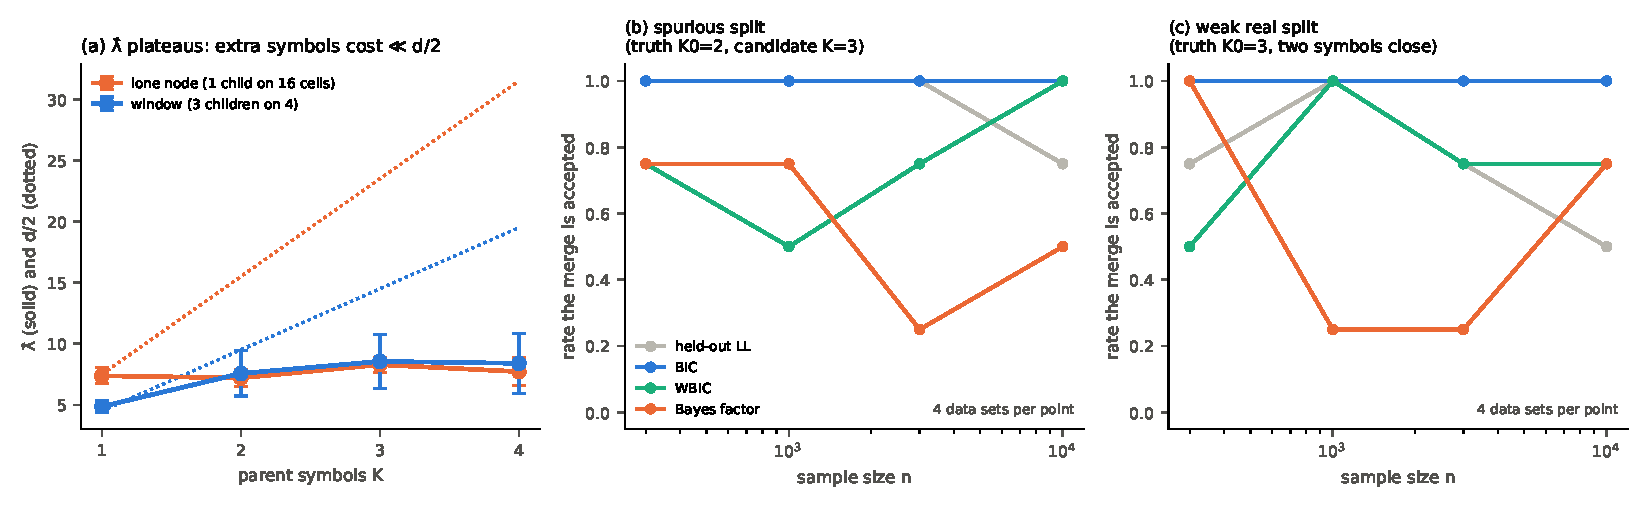
\includegraphics[width=\linewidth]{splitmerge_chart.pdf}
\caption{Split--merge and the learning coefficient.
(a) $\hat\lambda$ (solid, 95\% Monte-Carlo intervals) against $d/2$ (dotted) by the number of parent symbols, for a lone node (one child on 16 cells) and an identifying window (three children on 4); true $K_0=2$.
(b, c) How often each criterion accepts the merge back to $K_0$ for a spurious split (b) and a weak real split (c), over $n$ (4 data sets per point).}\label{fig:splitmerge}
\end{figure}

\textbf{Merge decisions in practice} (Figure~\ref{fig:splitmerge}b,c). We compare held-out likelihood, BIC, WBIC and the thermodynamic-integration Bayes factor, with four data sets per sample size.
\begin{itemize}
  \item For a \emph{spurious} split (truth $K_0=2$, candidate $K=3$), held-out likelihood and BIC reject the split at every $n$ from $300$ to $10^4$: the split loses $0.03$ to $0.0004$ nats per unit on held-out data.
  \item At our Monte-Carlo budget, WBIC and the Bayes factor are noisier and accept the merge in only $25$--$100\%$ of data sets. Their asymptotic advantage is offset by the error in estimating free energies in $30$--$40$ dimensions.
  \item A \emph{weak real} split (two of three true symbols $25\%$ apart) is not detectable by any criterion up to $n=10^4$: its held-out gain is $\approx0$.
  \item So the learning coefficient explains \emph{why} extra symbols are cheap and why the root is unlearnable, and it names the right criterion, the free energy. It does not, at feasible sample sizes and sampling budgets, beat held-out likelihood as a merge test.
\end{itemize}
An earlier suggestion to ``accept a merge iff it reduces the RLCT'' is not a criterion, since every merge does. Estimating per-level RLCTs on the O6 grammars themselves would require sampling hundreds of rule parameters per level; we leave that, with the caveat that WBIC is asymptotic and noisy for small corpora.

\subsection{Local window EM: learning one level at a time}\label{sec:localem}
The strata above suggest a gradient-free strategy that avoids global coupling: fit the hierarchy bottom up, one level at a time, from random starts, looking only at a local neighbourhood (\texttt{benchmarks/o6/local\_em.py}).
\begin{itemize}
  \item \emph{A lone node is not identifiable.} A node's child pair is a single categorical draw, and in a mixture of single draws, merging two symbols with usage weights is exactly free (the argument of Proposition~\ref{prop:root}; checked in \texttt{tests/test\_root\_identifiability.py}). The smallest identifying neighbourhood is a \emph{two-level window}, parent $\to$ (left, right) $\to$ child pairs, in which the sibling is the second view \cite{amr09}. Level $l$ is kept, the parent table is refitted in the next window, soft inside messages are passed up, and the root is one symbol (Proposition~\ref{prop:root}).
  \item \emph{Symmetry must be broken at the start, not annealed.} Tempered E-steps from $T_0=2$ drove every symbol to the same table, the symmetric fixed point exactly, which EM cannot leave (level-1 NMI $0.05$). Random Dirichlet starts at $T=1$ break the symmetry.
  \item \emph{Restarts land on merge strata.} At the upper levels the fitted symbols duplicate one another (held-out merge cost $\approx0$). A targeted local split--merge helps: merge the pair that the diagnostic finds redundant, split the most loaded symbol, and keep the change only if the held-out window likelihood improves. At $L=6$ this raised level-4 NMI from $0.16$ to $0.40$ and level-5 from $0.03$ to $0.23$.
\end{itemize}
NMI on the identifiable levels (test split, $N=20{,}000$):
\begin{center}\small
\begin{tabular}{lcccccc}
\toprule
$V=8$, $L=6$ & L1 & L2 & L3 & L4 & L5 & gap\\
\midrule
baseline (full split--merge) & $0.909$ & $0.970$ & $0.957$ & $0.794$ & $0.655$ & $0.005$\\
local window EM only & $0.901$ & $0.894$ & $0.663$ & $0.398$ & $0.229$ & $5.71$\\
local $+$ 60 global EM sweeps & $0.948$ & $0.923$ & $0.809$ & $0.593$ & $0.413$ & $1.75$\\
hybrid (local $+$ short split--merge) & $\mathbf{0.963}$ & $0.970$ & $0.957$ & $0.768$ & $\mathbf{0.668}$ & $0.049$\\
Bayes ceiling & $0.993$ & $0.970$ & $0.956$ & $0.866$ & $0.872$ & $0$\\
\midrule
$V=16$, $L=4$ & L1 & L2 & L3 & & & gap\\
\midrule
baseline & $0.983$ & $0.986$ & $0.810$ & & & $0.020$\\
local window EM only & $0.978$ & $0.934$ & $0.748$ & & & $0.79$\\
local $+$ 60 global EM sweeps & $\mathbf{0.987}$ & $0.981$ & $0.815$ & & & $0.28$\\
hybrid & $0.977$ & $0.982$ & $\mathbf{0.832}$ & & & $0.021$\\
\bottomrule
\end{tabular}
\end{center}
\begin{itemize}
  \item \emph{As an initialiser, local EM helps.} After 10 warm-up sweeps the hybrid is at a validation gap of $2.47$ nats, where the clustered initialisation needs 60 sweeps to reach $5.85$. With half the global split--merge budget (2 rounds instead of 4), the hybrid matches or beats the baseline's structure on most identifiable levels. The exceptions are L4 at $L=6$ and L1 at $V=16$. At $V=16$, local EM followed by 60 plain EM sweeps, with no global split--merge at all, already equals the baseline on levels 1--3.
  \item \emph{On its own it does not reach the top.} Going only deeper discards the top-down (outside) evidence, and errors compound upward: local-only NMI falls from $0.90$ at L1 to $0.23$ at L5. This agrees with the merge distances of Section~\ref{sec:gram-strata}, which shrink about $2.5$--$3\times$ per level.
  \item \emph{Cost.} The window E-step is $O(K^3)$ per node. The local fits cost more than the clustered initialisation, so the total time exceeds the baseline's. A sparse parent table is the obvious remedy.
\end{itemize}

\section{Massey products, and the $p$-adic and hierarchy loop tests}\label{sec:massey}
\textbf{Massey products} (\texttt{massey}). The averaged Shannon action is not multiplicative, which is why Vigneaux's cup product needs $F\otimes F$. The \emph{pointwise} action $(X.f)(P)(\omega)=f(P|_{X=X(\omega)})(\omega)$ is multiplicative, so local pointwise cochains form a differential graded algebra. The coboundary is Hochschild's,
\[
(\delta f)[X_1|\dots|X_{n+1}]=X_1.f[X_2|\dots]+\textstyle\sum_i(-1)^if[\dots|X_iX_{i+1}|\dots]+(-1)^{n+1}f[X_1|\dots|X_n],
\]
and the cup product is $(f\smile g)[X_1|\dots|X_{n+m}]=f[X_1|\dots|X_n]\cdot(X_1\cdots X_n).g[X_{n+1}|\dots]$.
\begin{proposition}[Surprisal is formal]\label{prop:massey}\st{proved; checked numerically}
Let $s[X](P)(\omega)=-\log P(X=X(\omega))$ and $u_n=s^n/n!$, both local 1-cochains. Then
\[
\delta u_n=-\sum_{i+j=n,\ i,j\ge1}u_i\smile u_j .
\]
Hence $s\smile s=-\delta u_2$ is a non-zero but exact cochain, and every Massey power $\langle s,\dots,s\rangle$ is defined and contains $0$. The $A_\infty$ structure generated by the surprisal is formal. The generating function of the defining system is $\sum_n u_n=e^{s}-1=1/P-1$.
\end{proposition}
\begin{proof}
With $a=\log P(x)$ and $b=\log P(y|x)$ we have $\delta(\log^nP)[X|Y]=b^n-(a+b)^n+a^n=-\sum_{0<i<n}\binom ni a^ib^{n-i}$, while $(u_i\smile u_j)[X|Y]=(-a)^i(-b)^j/(i!\,j!)$. Numerically, on three binary variables, the identity holds to $3\cdot10^{-14}$ for $n\le4$, the Leibniz rule to $3\cdot10^{-15}$, and $s\smile s$ has size $12.5$ (\texttt{tests/test\_massey.py}).
\end{proof}
\noindent On full-support laws the only class is $s$ (Proposition~\ref{prop:pwgraph}), so there are no non-trivial Massey products there. For $\alpha\ne1$ the pointwise Tsallis action $P(x)^{\alpha-1}f(P|x)$ is not multiplicative, so this DGA does not exist. The one non-trivial higher structure the paper does have is the arity of parse trees: faces of the associahedron correspond to planar trees, and a node of arity $k$ spans a cell of dimension $k-2$. These are combinatorial, not homotopical.

\textbf{The $p$-adic loop test} (\texttt{padic\_loops}). Take claims $x_i+x_j=r_{ij}$ in $\Z_p$.
\begin{proposition}[Sign twist and gluing radius]\label{prop:padicradius}\st{proved; checked}
\leavevmode
\begin{enumerate}
  \item The edge acts by $x\mapsto -x+r$, so the obstruction lives in $H^1$ with sign-twisted coefficients. An even cycle needs its alternating sum to vanish. An odd cycle is always solvable when $2$ is a unit ($p$ odd), and carries the parity obstruction when $p=2$.
  \item Let $m^*$ be the largest $m$ for which the system is solvable mod $p^m$, computed exactly by the Smith normal form over $\Z$. There is $x$ with $|x_i+x_j-r_{ij}|_p\le\rho$ for all claims iff $\rho\ge p^{-m^*}$. So the local Berkovich hulls glue exactly at radius $p^{-m^*}$, and on one even cycle $m^*=v_p(\text{alternating sum})$.
\end{enumerate}
\end{proposition}
Checks:
\begin{itemize}
  \item a 3-adic 4-cycle with alternating sum $1,3,9,27,54$ gives depths $0,1,2,3,3$;
  \item triangles always glue for $p=3$, and for $p=2$ fail exactly when $\sum r$ is odd;
  \item an error planted at digit $m$ of one claim on $K_8$ gives depth $m$, for $m=0,\dots,5$.
\end{itemize}
No gradients are needed: the system is linear over $\Z_p$ and is solved digit by digit.

\textbf{The hierarchy loop test.} A claim ``$i$ and $j$ meet at depth exactly $d$'' is realisable by a tree iff no claim $(i,j,d)$ has $i$ and $j$ already joined by claims all deeper than $d$. Equivalently, on every cycle the shallowest depth is attained at least twice (ultrametric). We check this by union-find in decreasing depth, with a witness path for each violation.
\begin{proposition}[Node-wise distortions are invisible]\label{prop:nodewise}\st{proved; checked}
If every claim's depth is changed by a function of its true meeting node only, no violation appears. The two shallowest claims on a cycle meet at the same node and move together. Detectable failures need item-level disagreement between sources. This is the hierarchy analogue of Proposition~\ref{prop:singlesource}.
\end{proposition}
\textbf{Synthetic test with graded arity} (\texttt{examples/hierarchy\_loops.py}). The tree has depth 5, and each node draws an arity in $\{2,3,4,5\}$. Two sources report exact meeting depths on random leaf pairs. Source~B misplaces 4 of 80 leaves, and only under odd-arity nodes.
\begin{itemize}
  \item Shifting every odd-arity node by one level gives $0$ violations.
  \item Noiseless, there are no false alarms. Every violation's witness touches a misplaced leaf and lies in the odd-arity grade.
  \item Detection of top-level misplacements rises with data: $0.10$, $0.33$, $0.82$ at $100$, $200$, $400$ claims per source. Deep misplacements are rarely seen ($\le0.07$), because only pairs meeting below that level can reveal them.
  \item Full results (100 runs per cell; the null 95th percentile matches the number of claims):
  \begin{center}\small
  \begin{tabular}{lcccccc}
  \toprule
  & \multicolumn{2}{c}{100 claims/source} & \multicolumn{2}{c}{200} & \multicolumn{2}{c}{400}\\
  misplacement level & 1 & 3 & 1 & 3 & 1 & 3\\
  \midrule
  detection, noise $0$ & $0.10$ & $0.00$ & $0.33$ & $0.01$ & $0.82$ & $0.03$\\
  detection, noise $0.05$ & $0.06$ & $0.09$ & $0.01$ & $0.04$ & $0.08$ & $0.05$\\
  detection, noise $0.10$ & $0.05$ & $0.04$ & $0.10$ & $0.04$ & $0.13$ & $0.06$\\
  \bottomrule
  \end{tabular}
  \end{center}
  Null violation means are $0$ without noise, $23$ / $174$ / $558$ at noise $0.05$, and $38$ / $215$ / $585$ at noise $0.10$, for $100$ / $200$ / $400$ claims. With noise, witness localisation is $0.21$--$0.32$ and the odd-grade share is $0.31$--$0.55$, against an odd-node base rate of $0.51$.
  \item With $5$--$10\%$ depth noise the violation count is dominated by noise: detection is $\le0.13$, and witness localisation falls to about $0.25$. A noise-robust version (for example an EM noise model, as in the contradiction meter) is open.
\end{itemize}

\section{Representations and perturbations: a summary}\label{sec:reppert}
This section collects what the paper now knows about how states are \emph{represented} in each layer, and how \emph{perturbations} act on them.

\textbf{Representations.}
\begin{itemize}
  \item \emph{Outcome layer (AMB):} a point's stratum, its support pattern, a face of the toric model (Section~\ref{sec:toricstrata}).
  \item \emph{Probability layer:} the position inside the stratum, a point of the toric model and of $\mathbf{FinStoch}$. It splits into a natural part (per-source and per-topic calibrations) and a loop part in $H^1$ (Section~\ref{sec:dynamics}).
  \item \emph{Operations:} representations of the fundamental groupoid of the cover. They land in $\R$ for bias loops, in permutation groups for label monodromy, and in $U(1)$ for phases (Sections~\ref{sec:mono}, \ref{sec:bias3}).
  \item \emph{Inside a filled cell:} the configuration of the $k$ values up to translation. Its shadow is the hull tree, or the variogram tree after leans are removed. For arithmetic data it is the Berkovich disc tree (Section~\ref{sec:hull}).
  \item \emph{Hierarchy:} a Kleisli morphism, a composite of rule kernels. It is defined up to relabelling, and the root is identifiable only as a mixture (Sections~\ref{sec:giry}, \ref{sec:gram-strata}).
\end{itemize}

\textbf{Perturbations and what they can move.}
\begin{itemize}
  \item \emph{Natural perturbations} (re-calibrations $u_s+v_t$) move only the natural part. They cannot change loops, variogram trees, or any outcome that reads only loops (Propositions~\ref{prop:natural}, \ref{prop:toggle}, \ref{prop:variogram}).
  \item \emph{Loop perturbations} move $H^1$ and can flip only outcomes that read loops (Proposition~\ref{prop:toggle}).
  \item \emph{Support perturbations} make the AMB layer jump ($\gamma$, $S_0$, the possibilistic outcome). Their exact cost is the mass of a co-facial set, and under gluing a single context never toggles alone (Proposition~\ref{prop:ambtoggle}).
  \item \emph{Second-order perturbations} change who agrees with whom while leaving every mean fixed. They can flip majority and AMB outcomes, and holonomy cannot see them (Proposition~\ref{prop:majority}).
  \item \emph{Continuity.} CF and the entropies move continuously through all of these, and only support-level quantities jump (Section~\ref{sec:gldyn}).
  \item \emph{Robustness.} The Weyl certificate bounds the perturbation a cover survives without tearing, and refinement tests separate obstructions from artefacts of the cover (Section~\ref{sec:certificate}).
  \item \emph{Invisible directions.} In grammar space, root merges are exactly invisible to the likelihood and upper-level merges almost so. These are the singular strata (Proposition~\ref{prop:root}).
\end{itemize}

\textbf{Measured on data.}
\begin{itemize}
  \item Flip costs in articles on a stream, and what drove each flip: rates, not topic mix (Section~\ref{sec:certificate}).
  \item Exact toggle radii (MBIC, AllSides).
  \item Paths over the gluing lattice: region choice alone can flip a held-out outcome for 44\% of MBIC targets, but outcome-driven region choice degrades accuracy by 55--65\%, while consistency-driven pruning improves it when regions are contaminated (Section~\ref{sec:latticepath}).
  \item Which layer moved at which event, and the outcome series against all layers (Section~\ref{sec:outcomeseries}).
  \item The outcome moves at some events (Charlottesville, Access Hollywood) without a corresponding change in coverage structure. Coverage does not lead the outcome at any lag up to 8 weeks.
\end{itemize}

\textbf{Not yet known.}
\begin{itemize}
  \item A causal or predictive link from coverage perturbations to the outcome. The present outcome series shows none.
  \item Perturbations of long-tailed rule probabilities (the tropical layer), which the current uniform-rule grammars cannot test.
  \item Non-abelian transports, where the character-variety picture would carry content.
  \item The perturbation theory of the local learner near the singular strata of grammar space.
\end{itemize}

\section{Detection: a map of the ideas and theorems}\label{sec:detmap}
\textbf{One idea.} A contradiction is a failure to glue locally consistent data. The meter keeps three failures apart:
\begin{itemize}
  \item \emph{self-contradiction}: a unit's support is empty;
  \item \emph{overlap disagreement}: $d^0\neq0$, the deficit;
  \item \emph{contextuality}: $d^0=0$ but $H^1\neq0$, which is ``locally consistent, globally inconsistent'' \cite{abramsky20}.
\end{itemize}

\begin{proposition}[Localisation]\label{prop:local}\src{S}\st{proved}
Let $g$ be an operation system with values in an abelian group $A$.
\begin{enumerate}
  \item On a cycle graph with holonomy $h\neq0$, for \emph{every} edge $e$ there is a flat system that differs from $g$ on $e$ alone, namely $g-h\,\mathbf 1_e$ with the orientation of $e$ along the cycle. So the edge data do not determine which edge is wrong. On a general graph, the minimal corrections to a flat system are likewise not unique.
  \item Declaring a spanning tree $T$ trusted removes the ambiguity. There is exactly one flat system that agrees with $g$ on $T$: its value on each cotree edge is the integral of $g$ along the tree path. The discrepancy sits on the cotree edges of the non-flat fundamental cycles.
\end{enumerate}
\end{proposition}
\begin{proof}
\begin{enumerate}
  \item Changing one edge of the cycle by $-h$ changes the holonomy by $-h$.
  \item A flat system is $\delta c$ for a potential $c$, and $\delta c=g$ on $T$ determines $c$ up to a constant.
\end{enumerate}
\end{proof}

\begin{table}[!htbp]\centering\small
\begin{tabular}{p{3.9cm}p{6.6cm}p{2.9cm}}
\toprule
role & result & where\\
\midrule
\multicolumn{3}{l}{\emph{What to detect}}\\
obstruction & AMB $\gamma$, ring-dependent; sufficient but not necessary (Hardy false negative) & \S\ref{sec:engine}\\
degree & contextual fraction (LP; the dual is a Bell inequality); $\CF=1$ iff strong & \S\ref{sec:engine}, \S\ref{sec:strata}\\
where $\gamma$ can be nonzero & support stratification; interior versus vertices & Prop.~\ref{prop:strata}\\
binary pairwise claims & all-or-nothing; odd $\Z/2$ cycle $=$ Liar $=$ PR box & Prop.~\ref{prop:two}\\
operations to outcomes & holonomy $[g]$ and the connecting class & Thm.~\ref{thm:eg}\\
cycles are necessary & acyclic and pairwise consistent implies global (BFMY; Vorob'ev) & Thm.~\ref{thm:vorobev}, \S\ref{sec:meter}\\
\midrule
\multicolumn{3}{l}{\emph{What cannot be detected}}\\
information lens & Layer-2 blindness to $[g]$ & Prop.~\ref{prop:blind-eg}\\
what it does read & moduli $|s_i|$; $\CF$ from moduli plus one bit & Prop.~\ref{prop:modphase}\\
falsehood & coherent fabrications have $\CF=0$ & \S\ref{sec:meter}\\
which edge & localisation needs a trusted tree & Prop.~\ref{prop:local}\\
long loops & girth bound $\ell_{\min}$ & Thm.~\ref{thm:girth}\\
\midrule
\multicolumn{3}{l}{\emph{How to compute}}\\
cheap $\CF$ bound & logical Bell bound $\sum p_i-(n-1)$ & Prop.~\ref{prop:lbell}\\
noisy cycles & closed form $1-|L|\varepsilon/2$ & Thm.~\ref{thm:cfcycle}\\
parity claims & Gaussian elimination over $\F_2$ with a certificate & \S\ref{sec:meter}\\
affine operations & dimension deficit $\operatorname{rank}(M-I)$; section count & \S\ref{sec:magphase}\\
dimension as a class & cocycle on affine supports over $\F_p$ & Prop.~\ref{prop:ffdim}\\
shortest contradictions & BFS in the parity double cover & \S\ref{sec:meter}\\
\midrule
\multicolumn{3}{l}{\emph{From samples}}\\
holonomy & Wald test with delta-method standard error; $N_{80}$ & \S\ref{sec:p26}\\
overlaps & deficit with a pinned bootstrap null; threshold sweep with a null band & \S\ref{sec:na}\\
meter & pooled flip rate by EM; Bonferroni over cycles & \S\ref{sec:meter}\\
real data & permutation null (BASIL) & \S\ref{sec:meter}\\
\bottomrule
\end{tabular}
\caption{The detection toolkit, with pointers to where each result is stated.}
\end{table}

\noindent\textbf{Design rules.}
\begin{enumerate}
  \item Build the cover from provenance, not from token distance.
  \item Record overlap disagreements; do not average them.
  \item Report cycles. Blame an edge only against a declared trusted set (Proposition~\ref{prop:local}).
  \item Read phase with loop quantities (holonomy, parity product, deficit), and magnitude with per-context information.
  \item Give every detector a planted positive and a null.
\end{enumerate}

%=====================================================================
\section{Net assessment: what the machinery adds, and what standard methods already give}\label{sec:net}
Almost every number in Sections~\ref{sec:giry}--\ref{sec:singular} can be reproduced with standard tools: linear programmes, log-linear models, regression and the bootstrap. The machinery adds three things:
\begin{itemize}
  \item which computation answers which question;
  \item proofs that some popular constructions cannot work;
  \item a short list of practical findings.
\end{itemize}
The second-order geometry mostly \emph{certified} that first-order models suffice on our data.

\begin{center}\small
\resizebox{\linewidth}{!}{\begin{tabular}{>{\raggedright\arraybackslash}p{0.17\linewidth}>{\raggedright\arraybackslash}p{0.3\linewidth}>{\raggedright\arraybackslash}p{0.22\linewidth}>{\raggedright\arraybackslash}p{0.27\linewidth}}
\toprule
piece & key outcome & reproducible by a standard method? & net gain\\
\midrule
Giry monad, $\mu$ vs adjunction (\ref{sec:giry}, \ref{sec:kernelpresheaf}) & gluing is a limit; $\mu$ enters only once a gluing is chosen & n/a & design guidance; corrects ``kernel presheaf / 2-group'' proposals\\
hull covers (\ref{sec:hullcover}) & useless for region choice; blind to direction & n/a & a negative result that stops a dead end\\
bounds over gluings (\ref{sec:bounds}) & coverage $0.97$--$1.00$; unanimity identified, ``all'' and ``majority'' not & yes: Fr\'echet / partial-identification LP & the identification rule ($f\perp\ker R$) and its link to loop content\\
grey contexts (\ref{sec:grey}) & MBIC age/gender stitching gives bounds $0.95$--$1$ wide; the independence point is right only by assumption & yes: statistical matching, ecological inference & shows how much of a what-if answer the assumption supplies\\
multi-conditionals (\ref{sec:multicond}) & number of independent conditions $=\dim\ker R$; pairs possible singly but not jointly & yes: LP feasibility & refutes the cup-product mask\\
population test (\ref{sec:bounds}) & AllSides centre--right shift ($p=2\times10^{-4}$), found three ways & yes: a $\chi^2$ test, once one knows to run it & \textbf{practical finding}; the machinery said where to look\\
sphere covers (\ref{sec:higher}) & a higher-order obstruction invisible to every pairwise or loop method; none in MBIC & partly: log-linear and Bell-inequality literature & instrumentation; a precise statement of the blind spot\\
toric [F][T][I][S] (\ref{sec:toricsphere}) & no top-order interaction in any corpus; max-ent accurate to $\le0.004$ & yes: log-linear interaction tests, Birch, IPF & certifies the standard gluing\\
curvature [C] (\ref{sec:curvature}) & Dem-affiliated house effect $-2.5$ points; the bend is $e$-flat & yes: the house effect is regression & certifies the linear model and first-order inference\\
deformations [D] (\ref{sec:deform}) & $T^2=0$; a flop at nodes; the toggle's pair flips in $18$--$55\%$ of resamples & the instability, yes, by bootstrap & explains it; shows the ``$\mathrm{Ext}^2$ obstruction'' does not exist\\
singular statistics [L] (\ref{sec:singular}) & toggle certainty overstated by $19$--$52$ points; BIC over-penalises latent classes; the polls' ``hidden component'' is $0.5\%$ outlying polls & partly: bootstrap, Bayes factors & correct penalties; a data-quality finding\\
split--merge and RLCT (\ref{sec:splitmerge-rlct}) & lone node and root contribute $0$; spurious splits cost about $1$, not $d/2$ & held-out likelihood already rejects spurious splits & explanation, not a better test at feasible $n$\\
arithmetic universe (Remark~\ref{rem:au}) & finitary vs analytic split of the engine & n/a & re-implementation guide; corrects ``a transformer is an AU''\\
\bottomrule
\end{tabular}}
\end{center}

\textbf{First- versus second-order extraction.}
\begin{itemize}
  \item \emph{First order} (loop content, $H^1$) carries the signal in our data: region influence ($R^2=0.89$), the population shift, the toggles.
  \item \emph{Second order} (top-order interaction, curvature, the $H^2$ of sphere covers, singular penalties) came back null or ``simple model adequate'' on every real table. The exceptions are the flop instability and singular model selection, where it changed the decision. Its value is certification.
\end{itemize}

\textbf{Cost.} Everything runs on CPU in seconds to minutes, with no gradient steps:
\begin{itemize}
  \item LP bounds take milliseconds per outcome, and their bootstrap validation about $9$ minutes;
  \item the toric and deformation components take about $10$ seconds each, curvature about $2$ minutes;
  \item the singular statistics take about $2$ minutes and split--merge about $15$ minutes of MCMC.
\end{itemize}
Exact programmes grow as $2^n$ global outcomes, so they are practical up to about $15$--$20$ binary measurements. Everything runs on count tables, which are sufficient statistics.

\textbf{Against transformer learning.} This comparison is structural; no transformer was trained on these tasks.
\begin{itemize}
  \item A transformer gives one prediction, i.e.\ one gluing with learned biases. By design it does not output bounds over all consistent joint laws, identification status, contextuality certificates, population-shift tests or curvature diagnostics.
  \item Section~\ref{sec:gram-strata} explains why the upper hierarchy levels are hard for \emph{any} learner: merge distances shrink toward $0$, and the root is unidentifiable.
  \item The two are complementary. A transformer is the natural upstream labeller (text to labels and features). The engine then checks consistency, bounds outcomes, locates obstructions, and certifies which simple model suffices.
\end{itemize}

\textbf{Where the novelty is.}
\begin{itemize}
  \item Practical findings: the centre--right population shift, the instability of toggle identity, and the outlying polls.
  \item Negative results: hull region choice, the cup-product mask, and $\mathrm{Ext}^2$ obstructions.
  \item The identifications: bound width is loop content; nodes produce flops; top-order structure is invisible to pairwise views. Each tells a reader when a standard method suffices and when it cannot.
\end{itemize}

\part{Status}
\section{Status of every claim}
\begin{itemize}
  \item \textbf{Proved:}
  \begin{itemize}
    \item T0 and its corollary; holonomy obstruction and connecting class;
    \item Propositions~8--10 of \src{O}; non-unification; vanishing (trivial action); Corollary~28;
    \item the $p$-adic proposition;
    \item identifiability (Prop.~\ref{prop:ident}) and its T0 corollary; the Chernoff bound;
    \item Theorem~\ref{thm:eg} and Layer-2 blindness; character eigenvalues;
    \item Theorem~\ref{thm:cfcycle}; the lower bound of Theorem~\ref{thm:girth};
    \item orientation on $\Z/3$ and $\Z/5$; convexity of KL balls and exact pair radii;
    \item $\Aff(\Z/p)$ invariants; the codimension formula;
    \item $R$ and $E$; the zero set of the deficit;
    \item support stratification (Proposition~\ref{prop:strata}); localisation (Proposition~\ref{prop:local}), its corollary, and two-outcome supports (Proposition~\ref{prop:two});
    \item the logical Bell bound (Proposition~\ref{prop:lbell}); the lower bound in Proposition~\ref{prop:modphase}; the identities in Remark~\ref{rem:grass}; dimension as a cocycle on affine supports over $\F_p$ (Proposition~\ref{prop:ffdim});
    \item O2 for the true grammar: Propositions~\ref{prop:o2a}, \ref{prop:o2b}, \ref{prop:o2d}, Theorem~\ref{thm:o2c}, and the root collapse;
    \item the band proposition (Proposition~\ref{prop:band}) and twist-invariance for symmetric local solutions (Proposition~\ref{prop:twistinv}); holonomy on the graph stratum with $\R^\Omega$ coefficients (Proposition~\ref{prop:pwgraph}), non-exact under Vigneaux locality; weak-edge contextuality without holonomy (Proposition~\ref{prop:weakedge}); the admissibility criterion (Corollary~\ref{cor:admiss}); two-sided acyclicity (Proposition~\ref{prop:twoside}); single-source consistency (Proposition~\ref{prop:singlesource}); formality of the surprisal (Proposition~\ref{prop:massey}); the $p$-adic gluing radius and sign twist (Proposition~\ref{prop:padicradius}); invisibility of node-wise distortions (Proposition~\ref{prop:nodewise}); filled cells are flat (Proposition~\ref{prop:filled}); naturality of phase changes (Proposition~\ref{prop:natural}); descent (Lemma~\ref{lem:descent}); toggle directions (Proposition~\ref{prop:toggle}); hull invariants of a filled cell and the $p$-adic order profile (Proposition~\ref{prop:hull}); the variogram tree (Proposition~\ref{prop:variogram}); majority reads the tree (Proposition~\ref{prop:majority}); the AMB toggle radius and Markov-move closure of co-facial sets (Proposition~\ref{prop:ambtoggle}); non-identifiability of the root level (Proposition~\ref{prop:root}); decoding as Bayesian inversion (Proposition~\ref{prop:bayesinv}); functoriality of mutual-information persistence (Proposition~\ref{prop:mipers}); region dependence is loop content (Proposition~\ref{prop:regioninv}); the first-order landscape (Proposition~\ref{prop:landscape}).
  \end{itemize}
  \item \textbf{Computed:}
  \begin{itemize}
    \item V0--V4a identities; $H^0$, $H^1$, $H^2$ of small semilattices;
    \item the mod-3 grid over five rings; possibilistic fragility; Hardy false negative;
    \item Baudot--Bennequin identities; the Tsallis $\delta_\alpha$ cocycle;
    \item Counterexamples~\ref{ce:info} and \ref{ce:o2}; the O2 rank table and root collapse;
    \item $Z^1$ of the operation-twisted Vigneaux complex on $\Z/3$ and $\Z/2$ cycles, and the $\R^\Omega$ table with the $O(\varepsilon)$ near-cocycle count (Section~\ref{sec:twisted}).
  \end{itemize}
  \item \textbf{Measured:}
  \begin{itemize}
    \item transformer negative; split--merge recovery; instrument calibrations;
    \item Wald calibration and $N_{80}$; equality in Theorem~\ref{thm:girth};
    \item wall absorption; $\Aff(\Z/5)$ recovery; graded-extension uniqueness;
    \item the gated-test table; deficit behaviour; ridge; threshold windows;
    \item grammar-guided transformers on Corpus B (Section~\ref{sec:exp1});
    \item equality in Proposition~\ref{prop:modphase} for $n=4$; the dimension deficit from estimated supports; $S_2$ versus Shannon estimation (no gain); the contradiction-meter benchmark (Section~\ref{sec:meter}); recursive-training collapse (Section~\ref{sec:collapse}); unknown branching with chunks and split--merge (Section~\ref{sec:vbranch}); monodromy and the local certificate phase (Section~\ref{sec:mono}, Proposition~\ref{prop:certphase}); the covariant perturbation split (Theorem~\ref{thm:split}); the R\'enyi deficit dial (Proposition~\ref{prop:renyi}); the O6 scaling ladder (Section~\ref{sec:o6}); three-level bias on BASIL, MBIC and NewsWCL50, arity-graded holonomy and phase change (Section~\ref{sec:bias3}).
  \end{itemize}
  \item \textbf{Open:}
  \begin{itemize}
    \item O1 identifiability threshold $\theta(V,L,\ell,m)$; O2 on fitted tables (statistical equality of upward rows); O4 power of $\beta_1$; O6 at $V=1024$, $L=16$ (benchmark and baseline in Section~\ref{sec:o6}; our baseline breaks at $V\approx64$--$128$ and $L\approx6$--$8$); O7 recurrent-depth transformers;
    \item Problems 21, 22 (23 blocked; 24 settled);
    \item $H^{\ge2}$ for $\delta$ and $\delta_\alpha$;
    \item the packing proof for Theorem~\ref{thm:girth}; an invariant separating noise from holonomy under non-covariant noise;
    \item integer-coefficient persistence for decorated barcodes;
    \item the conjecture that operations visible to Layer~2 are lossy and admit no \emph{cohomological} invariant. It is refuted in part: the loop spectrum is a non-cohomological invariant;
    \item extending the gated test to triple contexts;
    \item equality in Proposition~\ref{prop:modphase} for general $n$; the $\Z/n$ modulus--phase analogue; non-triviality of the dimension class; the deficit under non-covariant noise; the rank of $V_0$ for richer ans\"atze; the soft near-cocycle count on estimated (noisy) data; an escort-map Frobenius on the $\alpha$-complex (Remark~\ref{rem:hodge}); a twist-sensitive $H^1$ off the stratum (full support is blind in our ans\"atze).
  \end{itemize}
  \item \textbf{Withdrawn or corrected:}
  \begin{itemize}
    \item the embedding probe \src{H};
    \item ``$I_2=\delta H$'';
    \item the two-point entropy formula for noisy shifts;
    \item ``information bounds dictate CF'';
    \item ``the spectrum reads $h$'': it is the labelled eigenvalue;
    \item ``the optimal non-contextual part is generally not unique'': it depends on the scenario;
    \item ``deficit independent of CF'': it was then established by the sweep;
    \item a claim in the nerve module that non-identity bars die only at non-flat events: it fails for $\Z/2$ coefficients and non-abelian groups;
    \item the ``BBV'' expansion as a Bell-nonlocality framework: no such framework could be identified;
    \item the ``sheaf--geometric bridge'' $\chi(\gamma_{\mathrm{AMB}})=\operatorname{Hol}(\alpha,\partial M)$ and contextuality at single-outcome supports (Remark in Section~\ref{sec:strata});
    \item our prediction that linear labelled cocycles carry a twisted \v{C}ech part at $\alpha=1$: they vanish (Section~\ref{sec:twisted}); and our first exactness remark for $\R^\Omega$ coefficients, which holds only without locality in degree $0$.
  \end{itemize}
\end{itemize}

\section{The constructive core: the rational distribution monad in an arithmetic universe}\label{sec:constructive}
This section proves the construction sketched in Remark~\ref{rem:au}. Throughout, $\mathcal A$ is an arithmetic universe: a list-arithmetic pretopos \cite{joyal73,maietti10}, for example $\mathbf{Set}$ or the initial one. In $\mathcal A$ we have finite limits, disjoint and stable coproducts, effective quotients of equivalence relations, a natural numbers object $\mathbb N$, and a list object $L(Y)$ for every $Y$, with $\mathrm{nil}$, $\mathrm{cons}$ and its recursion principle. From $\mathbb N$ one builds $\mathbb Z$ and $\mathbb Q$ with decidable equality and order, and $\mathbb Q_{>0}$ is a decidable subobject of $\mathbb Q$. A transformer plays no role here (Remark~\ref{rem:au}). Statements marked \texttt{[exec]} are also checked in exact rational arithmetic in \texttt{amb\_vigneaux/constructive.py} and \texttt{tests/test\_constructive.py}.

\subsection*{Construction}
\begin{definition}[Finitely supported rational distributions]\label{def:dq}
For an object $X$ of $\mathcal A$, let $\sim$ be the equivalence relation on $L(X\times\mathbb Q_{>0})$ \emph{generated} by three moves:
\begin{itemize}
  \item[(P)] \emph{permutation}: swapping two adjacent entries;
  \item[(M)] \emph{merging}: $\ell_1\,(x,q)\,(x,r)\,\ell_2\sim\ell_1\,(x,q+r)\,\ell_2$;
  \item[(S)] \emph{scaling}: $(x_i,q_i)_i\sim(x_i,cq_i)_i$ for every $c\in\mathbb Q_{>0}$.
\end{itemize}
Put $\mathcal D(X)=L(X\times\mathbb Q_{>0})/{\sim}$, and write $[\![(x_1,q_1),\dots,(x_n,q_n)]\!]$ for a class, read as $\sum_iq_i\delta_{x_i}/\sum_iq_i$.
\end{definition}
\noindent The generated relation exists in $\mathcal A$, because transitive closures can be built with list objects \cite{maietti10}, and its quotient exists because quotients are effective. Two remarks on the choice of $\sim$:
\begin{itemize}
  \item A tempting alternative asks for a bijection between the entries of two lists with equal normalised weights. That is wrong: it separates $[(x,1),(x,1)]$ from $[(x,1)]$, which are the same distribution.
  \item Repairing it by comparing aggregated weight functions needs decidable equality on $X$, which a general AU does not provide. The generated relation needs no decidability.
\end{itemize}

\begin{lemma}[Normal form]\label{lem:nf}\st{proved; [exec]}
If $X$ has decidable equality, two lists are equivalent iff their normalised weight functions $x\mapsto\sum_{x_i=x}q_i/\sum_iq_i$ agree. So $\sim$ is decidable for finite $X$.
\end{lemma}
\begin{proof}
Each generator preserves the normalised weight function. Conversely, with decidable equality, (P) brings equal points together and (M) merges them, leaving one entry per point. Two such lists with the same normalised weight function list the same points, so they differ by a permutation (P) and a scaling (S).
\end{proof}

\begin{definition}[Functor, unit, multiplication]\label{def:dmonad}
For $f:X\to Y$ let $\mathcal D(f)[\![(x_i,q_i)]\!]=[\![(f(x_i),q_i)]\!]$ (map $f$ over the list). Let $\eta_X(x)=[\![(x,1)]\!]$. For a list $(\ell_i,q_i)_i$ of lists $\ell_i=(x_{ij},r_{ij})_j$, let
\[ \mu_X\big[\![([\![\ell_i]\!],q_i)_i]\!\big]=\big[\!\big[\big(x_{ij},\tfrac{q_i\,r_{ij}}{W\,V_i}\big)_{i,j}\big]\!\big],\qquad W=\textstyle\sum_iq_i,\ V_i=\sum_jr_{ij}. \]
All three are defined by list recursion (map, fold for the sums, concatenation), so they are morphisms of $\mathcal A$ once they are shown to respect $\sim$.
\end{definition}

\begin{lemma}[Lifting lists of classes]\label{lem:lift}\st{proved}
For an effective quotient $\pi:Y\to Y/E$, the map $L(\pi):L(Y)\to L(Y/E)$ is a regular epimorphism: every list of classes has a list of representatives.
\end{lemma}
\begin{proof}
Let $S\subseteq L(Y/E)$ be the image of $L(\pi)$.
\begin{itemize}
  \item $S$ contains $\mathrm{nil}$.
  \item $S$ is closed under $\mathrm{cons}$. The map $\pi\times L(\pi):Y\times L(Y)\to(Y/E)\times S$ is a regular epimorphism, since products of regular epis are regular epis in a regular category. And $\mathrm{cons}(\pi y,L(\pi)\ell)=L(\pi)(\mathrm{cons}(y,\ell))$ lies in $S$.
\end{itemize}
So $S$ is a sub-algebra of the initial $(1+(Y/E)\times-)$-algebra $L(Y/E)$, hence all of it.
\end{proof}

\begin{proposition}[Well defined]\label{prop:dwelldef}\st{proved; [exec]}
$\mathcal D(f)$ and $\mu_X$ respect $\sim$, and $\mu_X$ descends to $\mathcal D(\mathcal D(X))$. Hence $\mathcal D$ is an endofunctor of $\mathcal A$, and $\eta$ and $\mu$ are natural.
\end{proposition}
\begin{proof}
It suffices to check the generators.
\begin{itemize}
  \item $\mathcal D(f)$ commutes with (P) and (S), and sends (M) to (M) with the merged point $f(x)$.
  \item For $\mu_X$, on an inner list: (P) permutes the output, (M) merges two output entries, and (S) multiplies $r_{ij}$ and $V_i$ by the same $c$, so it leaves $r_{ij}/V_i$ unchanged.
  \item On the outer list: (P) permutes blocks; (S) cancels between $q_i$ and $W$; (M) merges two equal inner classes $[\![\ell_i]\!]=[\![\ell_k]\!]$, whose blocks are then equivalent after normalisation and merge by (M) entry by entry.
\end{itemize}
By Lemma~\ref{lem:lift}, the map from $L(L(X\times\mathbb Q_{>0})\times\mathbb Q_{>0})$ onto $\mathcal D(\mathcal D(X))$ is a composite of regular epimorphisms. A map constant on its fibres therefore factors through it. Naturality is $f(x_{ij})$ commuting with the formula.
\end{proof}

\begin{proposition}[Monad laws]\label{prop:dmonadlaws}\st{proved; [exec]}
\[ \mu_X\circ\eta_{\mathcal D X}=\mathrm{id},\qquad \mu_X\circ\mathcal D(\eta_X)=\mathrm{id},\qquad \mu_X\circ\mu_{\mathcal D X}=\mu_X\circ\mathcal D(\mu_X). \]
These are finitary equational identities over $\mathbb Q$.
\end{proposition}
\begin{proof}
On representatives:
\begin{itemize}
  \item $\mu(\eta(\ell))=(x_i,q_i/W)_i\sim\ell$ by (S).
  \item $\mu(\mathcal D(\eta)\ell)=(x_i,q_i\cdot1/(W\cdot1))_i\sim\ell$ by (S).
  \item For a three-level list with weights $p_i,q_{ij},r_{ijk}$ and sums $P,Q_i,R_{ij}$, both sides give the entries $\big(x_{ijk},\ p_iq_{ij}r_{ijk}/(P\,Q_iR_{ij})\big)$.
\end{itemize}
The check is executed on $200$ random nested lists in exact arithmetic.
\end{proof}

\begin{proposition}[Commutative and affine]\label{prop:dcommaff}\st{proved; [exec]}
With the strength $X\times\mathcal D(Y)\to\mathcal D(X\times Y)$, $(x,[\![(y_j,r_j)]\!])\mapsto[\![((x,y_j),r_j)]\!]$, the monad $\mathcal D$ is \emph{commutative}: both orders of forming the product law give $[\![((x_i,y_j),q_ir_j)]\!]$. It is also \emph{affine}: $\mathcal D(1)\cong1$.
\end{proposition}
\begin{proof}
The two double strengths list the same entries $((x_i,y_j),q_ir_j)$ in different orders, which (P) identifies. On $1\times\mathbb Q_{>0}$, (M) merges any list into $[(\ast,w)]$, and (S) sends it to $[(\ast,1)]$.
\end{proof}

\begin{theorem}[The probability layer is constructive]\label{thm:klmarkov}\st{proved}
$\mathrm{Kl}(\mathcal D)$, whose morphisms $X\to\mathcal D(Y)$ are finitely supported Markov kernels with rational weights, is a Markov category in Fritz's sense.
\end{theorem}
\begin{proof}
The Kleisli category of a commutative monad on a cartesian category is symmetric monoidal, with the product law of Proposition~\ref{prop:dcommaff} as tensor. Copy is $\eta\circ\Delta$ and discard is the unique map to $1$. Affineness makes discard natural, so the Kleisli category is a Markov category \cite{fritz}. The Kleisli category is not cartesian: the tensor is not a categorical product, and the unit is the terminal object of $\mathcal A$.
\end{proof}

\begin{definition}[Conditioning and the information action]\label{def:dcond}
For a decidable predicate $A$ on $X$ and $P=[\![(x_i,q_i)]\!]$ with $P(A)>0$ (decidable), let $P|_A=[\![(x_i,q_i)_{A(x_i)}]\!]$, i.e.\ filter and renormalise. For an observable $Z:X\to V$ with $V$ of decidable equality, Vigneaux's action on $F:\mathcal D(X)\to\mathbb Q$ is $(Z\cdot F)(P)=\sum_{v}P(Z=v)\,F(P|_{Z=v})$, the sum over the finitely many values in the support. Both are morphisms of $\mathcal A$. [exec: the Tsallis-$2$ cocycle identity $S_2(Z,Y)=S_2(Z)+\sum_vP(Z=v)^2S_2(Y\mid Z=v)$ holds exactly in $\mathbb Q$.]
\end{definition}

\subsection*{The boundary}
\begin{corollary}[What is finitary]\label{cor:finitary}
The following live in $\mathcal A$ and are computed exactly:
\begin{itemize}
  \item $\mathbb Q$, $\mathcal D$ and $\mathrm{Kl}(\mathcal D)$, conditioning and Vigneaux's action for observables with decidable equality;
  \item sufficient statistics, as deterministic maps with the Fisher--Neyman factorisation as an equation over $\mathbb Q$;
  \item the AMB support presheaf of a finite scenario and its \v{C}ech cohomology over $\mathbb Z$ and $\mathbb Z/n$ (Smith normal form);
  \item the contextual fraction of a \emph{rational} table and its Bell certificate (an LP over $\mathbb Q$ has a rational optimum, found by the finite simplex method);
  \item the toric ideal of a finite table and its Markov basis; facial sets, and the comparison of toggle costs through the forced masses;
  \item Tsallis entropies of integer order;
  \item $p$-adic valuations of rationals, hence the radius profile $e(m)$.
\end{itemize}
\end{corollary}

\begin{corollary}[What needs analysis]\label{cor:analytic}
The following do not live in $\mathcal A$:
\begin{itemize}
  \item $\mathbb R$, the Giry monad on measurable spaces, and continuous laws;
  \item Shannon entropy and the KL and R\'enyi divergences, even of rational laws, because they involve logarithms; hence toggle \emph{radii} $-\log(1-m)$, though not their order;
  \item the real points of a toric variety, IPF limits and the Birch point;
  \item eigenvalue certificates (Fiedler, Weyl), Slepian and multitaper methods;
  \item Berkovich spaces, which are completions;
  \item the estimation of curvature, learning coefficients and MCMC.
\end{itemize}
Some of these are real-algebraic: the Birch point solves polynomial equations over $\mathbb Q$, and eigenvalues are algebraic. They are decidable by real algebraic geometry, but they do not lie in $\mathbb Q$.
\end{corollary}

\begin{remark}[The boundary]\label{rem:boundary}
$\mathcal A$ carries the finitely supported, rational, count-based part of the engine: the outcome layer, the exact LP and MILP certificates, and the rational probability layer. Analysis enters at three points:
\begin{itemize}
  \item \emph{completion}: $\mathbb R$ and $\mathbb Q_p$;
  \item \emph{limits}: IPF, maximum entropy, asymptotic expansions;
  \item \emph{spectral data}: eigenvalues, tapers, curvature.
\end{itemize}
This is the left/right split of Remark~\ref{rem:au}, now with proofs.
\end{remark}

\section{Index of theorems and results}\label{sec:theoremindex}
This index lists every theorem-like statement in the paper, generated from the source, so the numbers are those of the statements themselves. The bracket gives each statement's status tag. Part A is the external results the work relies on: first those stated as theorems in Section~\ref{sec:theoremsused} and elsewhere, then those invoked in the text without a separate statement. Part B is the paper's own results, grouped by section.

\subsection*{A. External results used}
\noindent\emph{Stated in the paper:}
\begin{itemize}[itemsep=0pt]
  \item Thm.~\ref{thm:io} \emph{Inside--outside; Baker, Lari--Young} [used]
  \item Thm.~\ref{thm:em} \emph{EM ascent; Dempster--Laird--Rubin} [used]
  \item Thm.~\ref{res:auto1} \emph{Convergence; Wu} [used]
  \item Thm.~\ref{thm:vorobev} \emph{Extension; Vorob'ev} [used]
  \item Thm.~\ref{res:auto2} \emph{Independent pullback; Simpson Thm 6.4, Prop.~8.5} [used]
  \item Thm.~\ref{res:auto3} \emph{Conditional products; Fritz \S12} [used]
  \item Thm.~\ref{res:auto4} \emph{Sufficient statistics; Fritz Def.~14.3, Thm~14.5} [used]
  \item Thm.~\ref{res:auto5} \emph{Minimal sufficiency; Fritz Def.~16.2, Bahadur} [used]
  \item Thm.~\ref{thm:breg} \emph{Bregman information; Bregman, Banerjee et al.} [used]
  \item Thm.~\ref{thm:ostrowski} \emph{Ostrowski} [used]
  \item Thm.~\ref{thm:ew} \emph{Bregman TDA; Edelsbrunner--Wagner} [used]
  \item Thm.~\ref{thm:bb} \emph{Baudot--Bennequin} [used; verified numerically \src{S}]
\end{itemize}
\noindent\emph{Invoked in the text} (source; where used):
\begin{itemize}[itemsep=0pt]
  \item Abramsky--Brandenburger: no-signalling families are exactly the images of signed global measures; the sheaf-theoretic formulation \cite{ab11} (Proposition~\ref{prop:twoside}, Sections~\ref{sec:kernelpresheaf}, \ref{sec:bounds}).
  \item Contextual fraction as a linear programme, with its Bell-inequality dual \cite{abm17} (throughout; Section~\ref{sec:bounds}).
  \item Csisz\'ar: IPF converges to the $I$-projection when the fibre is non-empty \cite{csiszar} (Sections~\ref{sec:gldyn}, \ref{sec:bounds}, \ref{sec:toricsphere}).
  \item Fr\'echet bounds and partial identification \cite{frechet51,manski03}; Duncan--Davis ecological bounds \cite{duncandavis53} (Sections~\ref{sec:bounds}, \ref{sec:grey}).
  \item Charnes--Cooper linear-fractional programming \cite{charnescooper}; the conditional-independence assumption of statistical matching \cite{dorazio06} (Section~\ref{sec:grey}).
  \item Birch: the maximum-likelihood / maximum-entropy point of a log-linear model matches the margins \cite{birch63}; toric models and their facial sets \cite{gms06,fr12,efrs06} (Sections~\ref{sec:toricstrata}, \ref{sec:toricsphere}).
  \item Weyl's inequality for the Fiedler margin; Slepian and Thomson tapers \cite{slepian,thomson} (Sections~\ref{sec:certificate}, \ref{sec:slepian}).
  \item Cohen-Steiner--Edelsbrunner--Harer stability of persistence \cite{ceh}; data processing (Proposition~\ref{prop:mipers}). Comparison of experiments (Blackwell--Sherman--Stein) in categorical form \cite{fgpr20} (Section~\ref{sec:giry}).
  \item Weakly cartesian multiplication of the monad of a Markov category with conditionals \cite{bohinenperrone25} (Section~\ref{sec:giry}); de Finetti's theorem in categorical form \cite{fgp21} (Section~\ref{sec:singular}).
  \item Post-selection inference \cite{cox75,posi,fithian}; selection bias in model evaluation \cite{varma06,cawley10}; influence diagnostics \cite{cook77,bkw80} (Section~\ref{sec:latticepath}).
  \item Tree space, sticky means and energy tests \cite{bhv,hotz,szekely} (Section~\ref{sec:bhv}); identifiability of latent tree models \cite{amr09} (Section~\ref{sec:gram-strata}).
  \item Continuity of radius functions on Berkovich curves (only the elementary part) \cite{pulita} (Section~\ref{sec:hull}).
  \item Efron's statistical curvature \cite{efron75} (Section~\ref{sec:curvature}).
  \item Complete intersections are unobstructed ($T^2=0$) \cite{hartshorne10}; the conifold and its two small resolutions \cite{atiyah58} (Section~\ref{sec:deform}).
  \item Watanabe: RLCT as the pole of the zeta function, the free-energy expansion, Bayes generalisation error $\lambda/n$, WBIC \cite{watanabe,watanabe18,wbic}; thermodynamic integration \cite{gelmanmeng}; nuisance parameters present only under the alternative \cite{davies87} (Sections~\ref{sec:gram-strata}, \ref{sec:singular}, \ref{sec:splitmerge-rlct}).
  \item Frameworks shown \emph{not} to apply as proposed: non-abelian cohomology \cite{giraud,breen} (Remark~\ref{rem:nonabelian}); arithmetic universes as a model of a transformer \cite{joyal73,maietti10} (Remark~\ref{rem:au}). Higher and homotopical contextuality \cite{orbr17,kharoofokay} is where such extensions should attach.
\end{itemize}



\subsection*{B. Results of this paper, by section}
\noindent\textbf{The standing constraint}
\begin{itemize}[itemsep=0pt]
  \item Thm.~\ref{thm:T0} \emph{T0: single-source global section} [proved]
  \item Cor.~\ref{cor:T0} [proved]
\end{itemize}
\noindent\textbf{Framework: sites, presheaves, categories and schemes} (Section~\ref{sec:framework})
\begin{itemize}[itemsep=0pt]
  \item Prop.~\ref{prop:bayesinv} \emph{Decoding is Bayesian inversion} [proved; checked]
  \item Prop.~\ref{prop:mipers} \emph{Mutual-information persistence is functorial; HSIC persistence is not} [proved; checked]
  \item Prop.~\ref{prop:condprod} \emph{Conditional products glue trees, not cycles} [proved; checked]
  \item Prop.~\ref{prop:kerneladj} \emph{The adjunction, and why a linear one sees nothing} [proved; checked]
\end{itemize}
\noindent\textbf{Theorems and constructions used} (Section~\ref{sec:theoremsused})
\begin{itemize}[itemsep=0pt]
  \item Prop.~\ref{prop:padic} \emph{The lattice quasi-morphism does not exist} [proved, closed]
\end{itemize}
\noindent\textbf{The holonomy obstruction}
\begin{itemize}[itemsep=0pt]
  \item Thm.~\ref{thm:hol} \emph{Holonomy obstruction} [proved, computed]
  \item Thm.~\ref{thm:smooth} \emph{Holonomy as a connecting class} [proved]
  \item Prop.~\ref{res:auto6} \emph{T0 does not apply to operation systems}
  \item Prop.~\ref{res:auto7} \emph{Vorob'ev does not apply}
  \item Prop.~\ref{prop:frag} \emph{Possibilistic fragility does not apply} [computed]
\end{itemize}
\noindent\textbf{Non-unification and vanishing}
\begin{itemize}[itemsep=0pt]
  \item Thm.~\ref{thm:nonunif} \emph{Non-unification} [proved]
  \item Thm.~\ref{thm:vanish} \emph{Vanishing on the trivially-acting complex} [proved, computed]
  \item Cor.~\ref{res:auto8} \emph{Extensions do not help} [proved, closed]
\end{itemize}
\noindent\textbf{Problem 26: holonomy from estimated operations} (Section~\ref{sec:p26})
\begin{itemize}[itemsep=0pt]
  \item Prop.~\ref{prop:ident} \emph{Ring-theoretic identifiability} [proved, computed]
  \item Cor.~\ref{res:auto9} \emph{T0 for operations} [proved]
  \item Prop.~\ref{res:auto10} \emph{Calibrated test and sample cost} [measured; large-sample]
  \item Prop.~\ref{res:auto11} \emph{Discrete groups} [proved; measured looseness]
\end{itemize}
\noindent\textbf{From operations to outcomes, around the probability layer}
\begin{itemize}[itemsep=0pt]
  \item Thm.~\ref{thm:eg} \emph{The operation-system model $e_g$} [proved, computed]
  \item Prop.~\ref{prop:blind-eg} \emph{Layer 2 is blind to {$[g]$}} [proved]
\end{itemize}
\noindent\textbf{Lossy operations}
\begin{itemize}[itemsep=0pt]
  \item Prop.~\ref{prop:eig} \emph{Character eigenvalues} [proved]
  \item Cor.~\ref{res:auto12}
  \item Prop.~\ref{res:auto13} \emph{Information closed forms} [proved]
  \item Thm.~\ref{thm:cfcycle} \emph{Contextual fraction on a cycle} [proved]
  \item Thm.~\ref{thm:girth} \emph{Any graph, lower bound} [proved]
  \item Obs.~\ref{res:auto14} [measured]
  \item Prop.~\ref{res:auto15} \emph{Orientation for $\Z/3$ and $\Z/5$} [proved, computed]
\end{itemize}
\noindent\textbf{The support dial: Tsallis entropies} (Section~\ref{sec:tsallis})
\begin{itemize}[itemsep=0pt]
  \item Prop.~\ref{res:auto16} [computed; the cocycle property is Vigneaux's]
\end{itemize}
\noindent\textbf{Support strata: where each lens can see anything} (Section~\ref{sec:strata})
\begin{itemize}[itemsep=0pt]
  \item Prop.~\ref{prop:strata} \emph{Support stratification} [proved]
  \item Cor.~\ref{res:auto17} [proved]
  \item Prop.~\ref{prop:two} \emph{Two-outcome supports are all-or-nothing} [proved]
\end{itemize}
\noindent\textbf{Magnitude and phase: what Layer 2 reads} (Section~\ref{sec:magphase})
\begin{itemize}[itemsep=0pt]
  \item Prop.~\ref{prop:lbell} \emph{Logical Bell bound} [proved]
  \item Prop.~\ref{prop:modphase} \emph{$\CF$ from moduli and one bit} [lower bound proved; equality computed for $n=3,\dots,6$]
  \item Prop.~\ref{prop:ffdim} \emph{Dimension over $\F_p$} [proved; computed]
\end{itemize}
\noindent\textbf{The decorated Bregman--\v{C}ech nerve}
\begin{itemize}[itemsep=0pt]
  \item Lemma~\ref{res:auto18} [proved, computed]
  \item Prop.~\ref{res:auto19} \emph{Invariants for $\Aff(\Z/p)$} [proved]
  \item Prop.~\ref{prop:walls} \emph{Walls} [proved; consequence measured]
  \item Obs.~\ref{res:auto20} [measured]
\end{itemize}
\noindent\textbf{Two facets: restriction and extension} (Section~\ref{sec:functors})
\begin{itemize}[itemsep=0pt]
  \item Prop.~\ref{res:auto21} [proved, computed]
  \item Obs.~\ref{res:auto22} \emph{Graded extension} [measured]
\end{itemize}
\noindent\textbf{Not-applicable entries: the gated test} (Section~\ref{sec:na})
\begin{itemize}[itemsep=0pt]
  \item Prop.~\ref{res:auto23} \emph{The deficit} [proved (zero set); measured (the rest)]
  \item Obs.~\ref{res:auto24} \emph{The ridge} [measured]
  \item Obs.~\ref{res:auto25} \emph{Thresholded $\gamma$} [measured]
\end{itemize}
\noindent\textbf{O2: when is a merged model minimal sufficient?} (Section~\ref{sec:o2})
\begin{itemize}[itemsep=0pt]
  \item Prop.~\ref{prop:o2a} \emph{Lossless merges} [proved]
  \item Prop.~\ref{prop:o2b} \emph{The minimal sufficient statistic is a rank object} [proved]
  \item Thm.~\ref{thm:o2c} \emph{When a partition reaches the minimum} [proved]
  \item Prop.~\ref{prop:o2d} \emph{Bregman cost is a complete-data quantity} [proved]
  \item Cor.~\ref{res:auto26} \emph{The root collapses} [proved]
\end{itemize}
\noindent\textbf{Monodromy: representations of $\pi_1$ and twisted cohomology} (Section~\ref{sec:mono})
\begin{itemize}[itemsep=0pt]
  \item Prop.~\ref{prop:mono} \emph{What the representation adds} [proved; computed]
  \item Obs.~\ref{obs:grid} \emph{The mod-3 grid is not a loop-holonomy system} [computed]
  \item Prop.~\ref{prop:certphase} \emph{The local shadow: certificate phase} [proved; computed]
  \item Thm.~\ref{thm:split} \emph{Covariant perturbation split} [proved (1--4); 5 as stated]
\end{itemize}
\noindent\textbf{Bridges between $\mathcal F_{\Z}$ and $\mathcal F_\alpha$: the options} (Section~\ref{sec:bridges})
\begin{itemize}[itemsep=0pt]
  \item Prop.~\ref{prop:renyi} \emph{The R\'enyi deficit dial} [proved (i--iv); computed]
\end{itemize}
\noindent\textbf{The operation-twisted Vigneaux complex: a finite test} (Section~\ref{sec:twisted})
\begin{itemize}[itemsep=0pt]
  \item Prop.~\ref{prop:band} \emph{Band}
  \item Prop.~\ref{prop:twistinv} \emph{Coefficient twists are invisible}
  \item Prop.~\ref{prop:pwgraph} \emph{The probability layer reads the holonomy on the graph stratum}
  \item Cor.~\ref{cor:admiss} \emph{Fontaine-type reading; admissibility} [proved]
\end{itemize}
\noindent\textbf{Contextuality without holonomy: the weak edge} (Section~\ref{sec:weakedge})
\begin{itemize}[itemsep=0pt]
  \item Prop.~\ref{prop:weakedge} \emph{Weak-edge contextuality} [proved]
\end{itemize}
\noindent\textbf{Which coefficients can see contextuality} (Section~\ref{sec:coeffs})
\begin{itemize}[itemsep=0pt]
  \item Prop.~\ref{prop:twoside} \emph{Two-sided acyclicity} [(1)--(2) proved; (3) computed]
  \item Prop.~\ref{prop:singlesource} \emph{A single source always glues} [proved; checked on MBIC]
\end{itemize}
\noindent\textbf{Three-level bias: house lean, selective loops and global gluing} (Section~\ref{sec:bias3})
\begin{itemize}[itemsep=0pt]
  \item Prop.~\ref{prop:filled} \emph{Filled cells are flat} [proved; checked]
\end{itemize}
\noindent\textbf{Dynamics: phase changes as natural and non-natural transformations} (Section~\ref{sec:dynamics})
\begin{itemize}[itemsep=0pt]
  \item Prop.~\ref{prop:natural} \emph{Naturality of a phase change} [proved; module \texttt{dynamics}]
\end{itemize}
\noindent\textbf{Is the topology tearing? Descent, a spectral certificate, and outcome toggling} (Section~\ref{sec:certificate})
\begin{itemize}[itemsep=0pt]
  \item Lemma~\ref{lem:descent} \emph{Descent} [proved]
  \item Prop.~\ref{prop:toggle} \emph{Toggle directions}
  \item Prop.~\ref{prop:regioninv} \emph{Region dependence is loop content} [proved; checked]
  \item Prop.~\ref{prop:landscape} \emph{The landscape is first order, with the loop residuals as its slopes} [proved to first order; checked]
  \item Prop.~\ref{prop:hulldirection} \emph{Hulls are blind to direction} [proved; checked]
  \item Prop.~\ref{prop:bounds} \emph{Bounds over all gluings} [proved; checked]
  \item Prop.~\ref{prop:grey} \emph{Grey contexts} [proved; checked]
  \item Prop.~\ref{prop:multicond} \emph{Several conditionals} [proved; checked]
  \item Prop.~\ref{prop:higher} \emph{Covers whose nerve is a sphere} [proved; checked]
  \item Prop.~\ref{prop:birch} \emph{Fibre meets variety once} [proved; checked]
  \item Prop.~\ref{prop:deform} \emph{Deformations of the toric model} [proved; checked]
\end{itemize}
\noindent\textbf{Probing inside arity: hull trees and the $p$-adic radius profile} (Section~\ref{sec:hull})
\begin{itemize}[itemsep=0pt]
  \item Prop.~\ref{prop:hull} \emph{Hull invariants of a filled cell} [proved; checked]
  \item Prop.~\ref{prop:variogram} \emph{Variogram tree} [proved; checked]
  \item Prop.~\ref{prop:majority} \emph{Majority reads the tree} [proved; checked]
\end{itemize}
\noindent\textbf{Moduli: toric strata, tree space, and the singular strata of grammars} (Section~\ref{sec:moduli})
\begin{itemize}[itemsep=0pt]
  \item Prop.~\ref{prop:ambtoggle} \emph{AMB toggle radius} [proved; checked]
  \item Prop.~\ref{prop:root} \emph{The root level is not identifiable} [proved; checked]
  \item Prop.~\ref{prop:splitrlct} \emph{Learning coefficients at merge strata} [(1) proved; (2)--(3) computed]
\end{itemize}
\noindent\textbf{Massey products, and the $p$-adic and hierarchy loop tests} (Section~\ref{sec:massey})
\begin{itemize}[itemsep=0pt]
  \item Prop.~\ref{prop:massey} \emph{Surprisal is formal} [proved; checked numerically]
  \item Prop.~\ref{prop:padicradius} \emph{Sign twist and gluing radius} [proved; checked]
  \item Prop.~\ref{prop:nodewise} \emph{Node-wise distortions are invisible} [proved; checked]
\end{itemize}
\noindent\textbf{Detection: a map of the ideas and theorems} (Section~\ref{sec:detmap})
\begin{itemize}[itemsep=0pt]
  \item Prop.~\ref{prop:local} \emph{Localisation} [proved]
\end{itemize}
\noindent\textbf{The constructive core: the rational distribution monad in an arithmetic universe} (Section~\ref{sec:constructive})
\begin{itemize}[itemsep=0pt]
  \item Lemma~\ref{lem:nf} \emph{Normal form} [proved; [exec]]
  \item Lemma~\ref{lem:lift} \emph{Lifting lists of classes} [proved]
  \item Prop.~\ref{prop:dwelldef} \emph{Well defined} [proved; [exec]]
  \item Prop.~\ref{prop:dmonadlaws} \emph{Monad laws} [proved; [exec]]
  \item Prop.~\ref{prop:dcommaff} \emph{Commutative and affine} [proved; [exec]]
  \item Thm.~\ref{thm:klmarkov} \emph{The probability layer is constructive} [proved]
  \item Cor.~\ref{cor:finitary} \emph{What is finitary}
  \item Cor.~\ref{cor:analytic} \emph{What needs analysis}
\end{itemize}

\section{Method notes}
\begin{itemize}
  \item Every detector needs a planted positive and a null. The engine's T0 bug and the thresholded-$\gamma$ false positives were caught this way.
  \item Use Wasserstein, not bottleneck, distance for near-degenerate diagrams \src{H}.
  \item Plug-in MI bias is $(K-1)(L-1)/2N$; bootstrap nulls cancel it \src{H}.
  \item Read the proposition, not the summary.
\end{itemize}

\section{Reproduction}
\textbf{Code availability.} All code, tests, examples and this paper's source are at \url{https://github.com/vkawasth/Trainingless-Transformer-NoGradientDescent/tree/main/AMB-Vigneaux/}.
\begin{itemize}
  \item \src{H}: the command appendix of the hierarchy paper (\texttt{build\_corpus\_syn.py}, \texttt{splitmerge.py}, \texttt{estimator4.py}, \texttt{estimator6.py}).
  \item \src{O}: \texttt{holonomy.py}, \texttt{amb\_gamma.py}, \texttt{parity\_glue.py}, \texttt{h2\_rational.py}, \texttt{h2\_integral.py}.
  \item O6: \texttt{benchmarks/o6} (\texttt{o6\_generate.py}, \texttt{baseline\_splitmerge.py}, \texttt{o6\_score.py}; results and logs in \texttt{results/}, summary in \texttt{BASELINE.md}).
  \item \src{S}: \texttt{python -m pytest} (258 tests), \texttt{examples/holonomy\_estimated.py}, \texttt{examples/channels.py}, \texttt{examples/o2\_ranks.py}, \texttt{examples/o2\_verify.py}, \texttt{examples/train\_tf.py} with \texttt{grid.sh} (JAX), and modules \texttt{outcome}, \texttt{holonomy}, \texttt{channels}, \texttt{nerve}, \texttt{functors}, \texttt{na\_contexts}, \texttt{magphase}, \texttt{meter}, \texttt{meter\_general}, \texttt{monodromy}, \texttt{deficits}, \texttt{relclaims}, \texttt{twisted\_info}, \texttt{dynamics}, \texttt{spectral}, \texttt{certificate}, \texttt{toggle}, \texttt{hull}, \texttt{strata}, \texttt{treespace}, \texttt{giry}, \texttt{lattice\_path}, \texttt{kernel\_presheaf}, \texttt{bounds}, \texttt{higher}, \texttt{toric}, \texttt{curvature}, \texttt{deform}, \texttt{singular}.
\end{itemize}

\begin{thebibliography}{99}\small
\bibitem{ab11} S.~Abramsky, A.~Brandenburger. The sheaf-theoretic structure of non-locality and contextuality. \emph{New J.\ Phys.} 13:113036, 2011.
\bibitem{amb12} S.~Abramsky, S.~Mansfield, R.~S.~Barbosa. The cohomology of non-locality and contextuality. \emph{EPTCS} 95:1--14, 2012.
\bibitem{abklm15} S.~Abramsky, R.~S.~Barbosa, K.~Kishida, R.~Lal, S.~Mansfield. Contextuality, cohomology and paradox. \emph{CSL 2015}, LIPIcs 41.
\bibitem{abm17} S.~Abramsky, R.~S.~Barbosa, S.~Mansfield. Contextual fraction as a measure of contextuality. \emph{Phys.\ Rev.\ Lett.} 119:050504, 2017.
\bibitem{bb15} P.~Baudot, D.~Bennequin. The homological nature of entropy. \emph{Entropy} 17(5):3253--3318, 2015.
\bibitem{vig} J.~P.~Vigneaux. \emph{Topology of Statistical Systems}. PhD thesis, Universit\'e Paris Diderot, 2019.
\bibitem{vorobev} N.~N.~Vorob'ev. Consistent families of measures and their extensions. \emph{Theory Probab.\ Appl.} 7(2):147--163, 1962.
\bibitem{bfmy} C.~Beeri, R.~Fagin, D.~Maier, M.~Yannakakis. On the desirability of acyclic database schemes. \emph{J.\ ACM} 30(3):479--513, 1983.
\bibitem{cagnetta} F.~Cagnetta, L.~Petrini, U.~M.~Tomasini, A.~Favero, M.~Wyart. How deep neural networks learn compositional data: the Random Hierarchy Model. \emph{Phys.\ Rev.\ X} 14:031001, 2024.
\bibitem{dlr} A.~P.~Dempster, N.~M.~Laird, D.~B.~Rubin. Maximum likelihood from incomplete data via the EM algorithm. \emph{JRSS B} 39(1):1--38, 1977.
\bibitem{wu} C.~F.~J.~Wu. On the convergence properties of the EM algorithm. \emph{Ann.\ Statist.} 11(1):95--103, 1983.
\bibitem{baker} J.~K.~Baker. Trainable grammars for speech recognition. 1979. \quad K.~Lari, S.~J.~Young. \emph{Comp.\ Speech Lang.} 4(1):35--56, 1990.
\bibitem{simpson} A.~Simpson. Equivalence and conditional independence in atomic sheaf logic. arXiv:2405.11073, 2024.
\bibitem{fte} FiveThirtyEight. How popular is Donald Trump? Presidential approval poll list (approval\_polllist.csv, model date 2020-08-31), CC BY 4.0. Mirror: \url{https://github.com/kiranrangaraj/Trump-Tweets-and-Approval-Rating-ETL}.
\bibitem{econpolls} The Economist. 2020 US presidential forecast model, data/all\_polls.csv (2016 national polls from HuffPost Pollster). \url{https://github.com/TheEconomist/us-potus-model}.
\bibitem{cox75} D.~R.~Cox. A note on data-splitting for the evaluation of significance levels. \emph{Biometrika} 62(2):441--444, 1975.
\bibitem{cook77} R.~D.~Cook. Detection of influential observation in linear regression. \emph{Technometrics} 19(1):15--18, 1977.
\bibitem{bkw80} D.~A.~Belsley, E.~Kuh, R.~E.~Welsch. \emph{Regression Diagnostics: Identifying Influential Data and Sources of Collinearity}. Wiley, 1980.
\bibitem{varma06} S.~Varma, R.~Simon. Bias in error estimation when using cross-validation for model selection. \emph{BMC Bioinformatics} 7:91, 2006.
\bibitem{cawley10} G.~C.~Cawley, N.~L.~C.~Talbot. On over-fitting in model selection and subsequent selection bias in performance evaluation. \emph{J.\ Mach.\ Learn.\ Res.} 11:2079--2107, 2010.
\bibitem{posi} R.~Berk, L.~Brown, A.~Buja, K.~Zhang, L.~Zhao. Valid post-selection inference. \emph{Ann.\ Statist.} 41(2):802--837, 2013.
\bibitem{fithian} W.~Fithian, D.~Sun, J.~Taylor. Optimal inference after model selection. arXiv:1410.2597, 2014.
\bibitem{giry} M.~Giry. A categorical approach to probability theory. In \emph{Categorical Aspects of Topology and Analysis}, Lecture Notes in Math.\ 915, 68--85, Springer, 1982.
\bibitem{ceh} D.~Cohen-Steiner, H.~Edelsbrunner, J.~Harer. Stability of persistence diagrams. \emph{Discrete Comput.\ Geom.} 37(1):103--120, 2007.
\bibitem{fritz} T.~Fritz. A synthetic approach to Markov kernels, conditional independence and theorems on sufficient statistics. \emph{Adv.\ Math.} 370:107239, 2020.
\bibitem{wright} G.~Wright. An algebraic perspective on computing with data. PhD thesis, 2023.
\bibitem{banerjee} A.~Banerjee, S.~Merugu, I.~S.~Dhillon, J.~Ghosh. Clustering with Bregman divergences. \emph{JMLR} 6:1705--1749, 2005.
\bibitem{kemeny} J.~G.~Kemeny, J.~L.~Snell. \emph{Finite Markov Chains}. Van Nostrand, 1960.
\bibitem{slonim} N.~Slonim, N.~Tishby. Agglomerative information bottleneck. NIPS 1999.
\bibitem{petrov} S.~Petrov, L.~Barrett, R.~Thibaux, D.~Klein. Learning accurate, compact, and interpretable tree annotation. ACL 2006.
\bibitem{ew} H.~Edelsbrunner, H.~Wagner. Topological data analysis with Bregman divergences. SoCG 2017.
\bibitem{ostrowski} A.~Ostrowski. \"Uber einige L\"osungen der Funktionalgleichung $\varphi(x)\varphi(y)=\varphi(xy)$. \emph{Acta Math.} 41:271--284, 1916.
\bibitem{mm} G.~A.~Miller. Note on the bias of information estimates. 1955.
\bibitem{brunner} N.~Brunner, D.~Cavalcanti, S.~Pironio, V.~Scarani, S.~Wehner. Bell nonlocality. \emph{Rev.\ Mod.\ Phys.} 86:419, 2014.
\bibitem{bc90} S.~L.~Braunstein, C.~M.~Caves. Wringing out better Bell inequalities. \emph{Ann.\ Phys.} 202:22--56, 1990.
\bibitem{abramsky20} S.~Abramsky. Contextuality: at the borders of paradox. arXiv:2011.04899, 2020.
\bibitem{basil} L.~Fan, M.~White, E.~Sharma, R.~Su, P.~K.~Choubey, R.~Huang, L.~Wang. In plain sight: media bias through the lens of factual reporting. \emph{EMNLP 2019}.
\bibitem{vdgg} W.~van Dam, R.~D.~Gill, P.~D.~Gr\"unwald. The statistical strength of nonlocality proofs. \emph{IEEE Trans.\ Inf.\ Theory} 51(8):2812--2835, 2005.
\bibitem{ud} M.-C.~de Marneffe, C.~D.~Manning, J.~Nivre, D.~Zeman. Universal Dependencies. \emph{Computational Linguistics} 47(2):255--308, 2021. English-EWT treebank: \texttt{github.com/UniversalDependencies/UD\_English-EWT}.
\bibitem{korepanov} I.~G.~Korepanov, N.~M.~Sadykov. Parameterizing the simplest Grassmann--Gaussian relations for Pachner move 3--3. \emph{SIGMA} 9:053, 2013. arXiv:1305.3246v2, doi:10.3842/SIGMA.2013.053.
\bibitem{hansenli} D.~Hansen, S.~Li. Line bundles on rigid varieties and Hodge symmetry. arXiv:1708.08506v2, 2020.
\bibitem{mbic} T.~Spinde, L.~Rudnitckaia, K.~Sinha, F.~Hamborg, B.~Gipp, K.~Donnay. MBIC -- A media bias annotation dataset including annotator characteristics. \emph{iConference} 2021; arXiv:2105.11910. Raw labels from the BABE repository, \url{https://github.com/Media-Bias-Group/Neural-Media-Bias-Detection-Using-Distant-Supervision-With-BABE}.
\bibitem{newswcl50} F.~Hamborg, A.~Zhukova, B.~Gipp. Automated identification of media bias by word choice and labeling in news articles. \emph{JCDL} 2019. Data: \url{https://github.com/fhamborg/NewsWCL50}.
\bibitem{diaconis} P.~Diaconis, B.~Sturmfels. Algebraic algorithms for sampling from conditional distributions. \emph{Ann.\ Statist.} 26(1):363--397, 1998.
\bibitem{dss} M.~Drton, B.~Sturmfels, S.~Sullivant. \emph{Lectures on Algebraic Statistics}. Oberwolfach Seminars 39, Birkh\"auser, 2009.
\bibitem{baly} R.~Baly, G.~Da San Martino, J.~Glass, P.~Nakov. We can detect your bias: predicting the political ideology of news articles. \emph{EMNLP} 2020. Data: \url{https://github.com/ramybaly/Article-Bias-Prediction}.
\bibitem{slepian} D.~Slepian. Prolate spheroidal wave functions, Fourier analysis, and uncertainty V: the discrete case. \emph{Bell Syst.\ Tech.\ J.} 57(5):1371--1430, 1978.
\bibitem{thomson} D.~J.~Thomson. Spectrum estimation and harmonic analysis. \emph{Proc.\ IEEE} 70(9):1055--1096, 1982.
\bibitem{pulita} A.~Pulita. Infinitesimal deformation of $p$-adic differential equations on Berkovich curves. arXiv:0802.1945v5.
\bibitem{lurieSAG} J.~Lurie. \emph{Spectral Algebraic Geometry}. Book manuscript, version of February 2018. \url{https://www.math.ias.edu/~lurie/papers/SAG-rootfile.pdf}.
\bibitem{gms06} D.~Geiger, C.~Meek, B.~Sturmfels. On the toric algebra of graphical models. \emph{Ann.\ Statist.} 34(3):1463--1492, 2006.
\bibitem{fr12} S.~E.~Fienberg, A.~Rinaldo. Maximum likelihood estimation in log-linear models. \emph{Ann.\ Statist.} 40(2):996--1023, 2012.
\bibitem{efrs06} N.~Eriksson, S.~E.~Fienberg, A.~Rinaldo, S.~Sullivant. Polyhedral conditions for the nonexistence of the MLE for hierarchical log-linear models. \emph{J.\ Symbolic Comput.} 41(2):222--233, 2006.
\bibitem{sullivant} S.~Sullivant. \emph{Algebraic Statistics}. Graduate Studies in Mathematics 194, AMS, 2018.
\bibitem{fulton} W.~Fulton. \emph{Introduction to Toric Varieties}. Annals of Mathematics Studies 131, Princeton, 1993.
\bibitem{cls} D.~A.~Cox, J.~B.~Little, H.~K.~Schenck. \emph{Toric Varieties}. Graduate Studies in Mathematics 124, AMS, 2011.
\bibitem{bhv} L.~J.~Billera, S.~P.~Holmes, K.~Vogtmann. Geometry of the space of phylogenetic trees. \emph{Adv.\ Appl.\ Math.} 27(4):733--767, 2001.
\bibitem{speyer} D.~Speyer, B.~Sturmfels. The tropical Grassmannian. \emph{Adv.\ Geom.} 4(3):389--411, 2004.
\bibitem{acp} D.~Abramovich, L.~Caporaso, S.~Payne. The tropicalization of the moduli space of curves. \emph{Ann.\ Sci.\ \'Ec.\ Norm.\ Sup\'er.} 48(4):765--809, 2015.
\bibitem{devadoss} S.~L.~Devadoss. Tessellations of moduli spaces and the mosaic operad. \emph{Contemp.\ Math.} 239:91--114, 1999.
\bibitem{hotz} T.~Hotz, S.~Huckemann, H.~Le, J.~S.~Marron, J.~C.~Mattingly, E.~Miller, J.~Nolen, M.~Owen, V.~Patrangenaru, S.~Skwerer. Sticky central limit theorems on open books. \emph{Ann.\ Appl.\ Probab.} 23(6):2238--2258, 2013.
\bibitem{szekely} G.~J.~Sz\'ekely, M.~L.~Rizzo. Energy statistics: a class of statistics based on distances. \emph{J.\ Statist.\ Plann.\ Inference} 143(8):1249--1272, 2013.
\bibitem{watanabe} S.~Watanabe. \emph{Algebraic Geometry and Statistical Learning Theory}. Cambridge University Press, 2009.
\bibitem{watanabe18} S.~Watanabe. \emph{Mathematical Theory of Bayesian Statistics}. CRC Press, 2018.
\bibitem{golubtsov02} P.~V.~Golubtsov. Monoidal Kleisli category as a background for information transformers theory. \emph{Information Processes} 2(1):62--84, 2002.
\bibitem{fgpr20} T.~Fritz, T.~Gonda, P.~Perrone, E.~F.~Rischel. Representable Markov categories and comparison of statistical experiments in categorical probability. arXiv:2010.07416, 2020.
\bibitem{fgp21} T.~Fritz, T.~Gonda, P.~Perrone. De Finetti's theorem in categorical probability. arXiv:2105.02639, 2021.
\bibitem{bohinenperrone25} M.~Bohinen, P.~Perrone. Categorical algebra of conditional probability. arXiv:2502.14941, 2025.
\bibitem{wbic} S.~Watanabe. A widely applicable Bayesian information criterion. \emph{J.\ Mach.\ Learn.\ Res.} 14:867--897, 2013.
\bibitem{amr09} E.~S.~Allman, C.~Matias, J.~A.~Rhodes. Identifiability of parameters in latent structure models with many observed variables. \emph{Ann.\ Statist.} 37(6A):3099--3132, 2009.
\bibitem{giraud} J.~Giraud. \emph{Cohomologie non ab\'elienne}. Grundlehren 179, Springer, 1971.
\bibitem{breen} L.~Breen. On the classification of 2-gerbes and 2-stacks. \emph{Ast\'erisque} 225, 1994.
\bibitem{orbr17} C.~Okay, S.~Roberts, S.~D.~Bartlett, R.~Raussendorf. Topological proofs of contextuality in quantum mechanics. \emph{Quantum Inf.\ Comput.} 17(13--14):1135--1166, 2017.
\bibitem{kharoofokay} C.~Okay, A.~Kharoof, S.~Ipek. Simplicial quantum contextuality. \emph{Quantum} 7:1009, 2023.
\bibitem{frechet51} M.~Fr\'echet. Sur les tableaux de corr\'elation dont les marges sont donn\'ees. \emph{Ann.\ Univ.\ Lyon, Sect.\ A} 14:53--77, 1951.
\bibitem{manski03} C.~F.~Manski. \emph{Partial Identification of Probability Distributions}. Springer, 2003.
\bibitem{charnescooper} A.~Charnes, W.~W.~Cooper. Programming with linear fractional functionals. \emph{Naval Res.\ Logist.\ Q.} 9(3--4):181--186, 1962.
\bibitem{dorazio06} M.~D'Orazio, M.~Di~Zio, M.~Scanu. \emph{Statistical Matching: Theory and Practice}. Wiley, 2006.
\bibitem{duncandavis53} O.~D.~Duncan, B.~Davis. An alternative to ecological correlation. \emph{Amer.\ Sociol.\ Rev.} 18(6):665--666, 1953.
\bibitem{birch63} M.~W.~Birch. Maximum likelihood in three-way contingency tables. \emph{J.\ R.\ Stat.\ Soc.\ B} 25(1):220--233, 1963.
\bibitem{efron75} B.~Efron. Defining the curvature of a statistical problem (with applications to second order efficiency). \emph{Ann.\ Statist.} 3(6):1189--1242, 1975.
\bibitem{hartshorne10} R.~Hartshorne. \emph{Deformation Theory}. Graduate Texts in Mathematics 257, Springer, 2010.
\bibitem{atiyah58} M.~F.~Atiyah. On analytic surfaces with double points. \emph{Proc.\ R.\ Soc.\ Lond.\ A} 247:237--244, 1958.
\bibitem{gelmanmeng} A.~Gelman, X.-L.~Meng. Simulating normalizing constants: from importance sampling to bridge sampling to path sampling. \emph{Statist.\ Sci.} 13(2):163--185, 1998.
\bibitem{davies87} R.~B.~Davies. Hypothesis testing when a nuisance parameter is present only under the alternative. \emph{Biometrika} 74(1):33--43, 1987.
\bibitem{joyal73} A.~Joyal. Arithmetic universes. Unpublished lectures, 1973.
\bibitem{maietti10} M.~E.~Maietti. Joyal's arithmetic universe as list-arithmetic pretopos. \emph{Theory Appl.\ Categ.} 24(3):39--83, 2010.
\bibitem{csiszar} I.~Csisz\'ar. $I$-divergence geometry of probability distributions and minimization problems. \emph{Ann.\ Probab.} 3(1):146--158, 1975.
\end{thebibliography}
\end{document}
